\chapter{Speaker Single Tone Test} \label{app:journal_speaker_test2}

This test examines multiple single tones at different sound pressure levels until the loudspeaker distorts the sound by a significant amount. By only playing at one frequency, a high resolution graph of the frequency response can be achieved because of the large sample size, to determine if there is a correlation between the fundamental frequency and the second and third harmonic wave at different sound levels.


\section{Setup}

The setup of this experiment are depicted in Figure \ref{figure:SpeakertestSetup}, where the equipment is catalogued in \autoref{tab:UsedEquipment1}, and described as follows:

\begin{itemize}
\item Distortion and \gls{SPL} will be measured by a microphone at a distance 1 meter in accordance with IEC 60268-5 Sound System Equipment - Part 5: Loudspeaker.
\item Vibration will be measured by a Brüel \& Kjear Type 4344 accelerometer, placed at:
\begin{itemize}
\item The backplate of the lowest woofer
\item High, inside and on the back of the enclosure 
\end{itemize}
\item Vibration will also be measured by a ADXL335 accelerometer, placed in the same area (maximum 3 cm away) as the Brüel \& Kjear accelerometers. 
\item The speaker will be driven by a Crown Studio Reference I amplifier.
\item The ADC/DAC will convert measurements from accelerometers and microphone and relay to a computer via SPDIF.
\begin{itemize}
\item Both Accelerometers and Microphone is calibrated into outputting -37 dB at respectively 1 G and 94 dB \gls{SPL}.
\item All recordings are synchronised and timestamped with by looping the test file back into the converter.
\end{itemize}
\item The computer will be logging data with a RME HammerFall DIGI 96-PDST sound card and Adobe Audition.
\end{itemize}

Furthermore the speaker will be placed in the anechoic room to eliminate any external disturbances corresponding to the requirements demanded in the 
IEC 60268-5 standard.

\subsection*{Test Setup}

\begin{figure}[H]
\centering
%\tikzsetnextfilename{TestSetup1}
%\scalebox{0.7}{
%\begin{tikzpicture}
\node[input] (SpeakerCorner) at (0,0) {};
\node[PreAmpBox] (AMP0) at ($(6,-1.5)+(SpeakerCorner)$) {\scalebox{0.5}{Pre-amp}} ;
\node[PreAmpBox] (AMP1) at ($(0,-1)+(AMP0)$) {\scalebox{0.5}{Pre-amp}} ;
\node[PreAmpBox] (AMP2) at ($(0,-1)+(AMP1)$) {\scalebox{0.5}{Pre-amp}} ;
%\node[PreAmpBox] (AMP3) at ($(0,-1)+(AMP2)$) {\scalebox{0.5}{Pre-amp}} ;
%\node[PreAmpBox] (AMP4) at ($(0,-1)+(AMP3)$) {\scalebox{0.5}{Pre-amp}} ;
%\node[PreAmpBox] (AMP5) at ($(0,-1)+(AMP4)$) {\scalebox{0.5}{Pre-amp}} ;


%% Speaker Enclosure %%
%% Speaker %%
\draw[thick, fill=black!20] (SpeakerCorner) -- ($(2,0)+(SpeakerCorner)$) -- ($(2,-6)+(SpeakerCorner)$) -- ($(0,-6)+(SpeakerCorner)$) -- (SpeakerCorner);

\node[input] (Tweeter) at ($(0,-0.5)+(SpeakerCorner)$) {};
\draw[thick, fill=black!20] (Tweeter) -- ($(0,0.3)+(Tweeter)$) -- ($(0.5,0.25)+(Tweeter)$) -- ($(0.5,-0.25)+(Tweeter)$) -- ($(0,-0.3)+(Tweeter)$) -- (Tweeter);
\draw[thick, fill=black!20] ($(0.51,-0.25)+(Tweeter)$) -- ($(0.75,-0.25)+(Tweeter)$) -- ($(0.75,0.25)+(Tweeter)$) -- ($(0.51,0.25)+(Tweeter)$);

\node[input] (Speaker2) at ($(0,-2)+(SpeakerCorner)$) {};
\draw[thick, fill=black!20] (Speaker2) -- ($(0,0.5)+(Speaker2)$) -- ($(0.5,0.25)+(Speaker2)$) -- ($(0.5,-0.25)+(Speaker2)$) -- ($(0,-0.5)+(Speaker2)$) -- (Speaker2);
\draw[thick, fill=black!20] ($(0.51,-0.25)+(Speaker2)$) -- ($(0.75,-0.25)+(Speaker2)$) -- ($(0.75,0.25)+(Speaker2)$) -- ($(0.51,0.25)+(Speaker2)$);

\node[input] (Speaker) at ($(0,-3.5)+(SpeakerCorner)$) {};
\draw[thick, fill=black!20] (Speaker) -- ($(0,0.5)+(Speaker)$) -- ($(0.5,0.25)+(Speaker)$) -- ($(0.5,-0.25)+(Speaker)$) -- ($(0,-0.5)+(Speaker)$) -- (Speaker);
\draw[thick, fill=black!20] ($(0.51,-0.25)+(Speaker)$) -- ($(0.75,-0.25)+(Speaker)$) -- ($(0.75,0.25)+(Speaker)$) -- ($(0.51,0.25)+(Speaker)$);

\draw[thick, fill=black!20] ($(2,-5.5)+(SpeakerCorner)$) -- ($(1,-5.5)+(SpeakerCorner)$) -- ($(1,-5)+(SpeakerCorner)$) -- ($(2,-5)+(SpeakerCorner)$) -- ($(2,-5.5)+(SpeakerCorner)$);

%% Computer + AMP %%
\begin{pgfonlayer}{bg}
\node[input] (ComputerCorner) at (8,-1) {};
\draw[thick, fill=black!20] (ComputerCorner) -- ($(2,0)+(ComputerCorner)$) -- ($(2,-4)+(ComputerCorner)$) -- ($(0,-4)+(ComputerCorner)$) -- (ComputerCorner);
\end{pgfonlayer}{bg}

\node[] (Computer) at ($(1,-2)+(ComputerCorner)$) {ADC/DAC};

\node[PreAmpBox] (AMP) at ($(1,-5)+(ComputerCorner)$) {\scalebox{0.5}{Amplifier}} ;

%% Draw Lines %%

%% Pre-amp to Speaker
\draw[<-,mark=*] (AMP0) -- ($(-3,0)+(AMP0)$) |- ($(-1.5,0.5)+(SpeakerCorner)$) -- ($(-1.5,-2)+(SpeakerCorner)$) ;
\draw [red,fill] ($(-1.5,-2)+(SpeakerCorner)$) circle [radius=0.1];

\draw[<-,mark=*] (AMP1) -| ($(-4.25,1.5)+(AMP1)$) ;
\draw [blue,fill] ($(-4.25,1.5)+(AMP1)$) circle [radius=0.1];

\draw[<-,mark=*] (AMP2) -- ($(-5.25,-0)+(AMP2)$) ;
\draw [blue,fill] ($(-5.25,-0)+(AMP2)$) circle [radius=0.1];

%\draw[<-,mark=*] (AMP3) -- ($(-5.5,0)+(AMP3)$) ;
%\draw [blue,fill] ($(-5.5,0)+(AMP3)$) circle [radius=0.1];

%\draw[<-,mark=*] (AMP4) -- ($(-4.5,0)+(AMP4)$) ;
%\draw [blue,fill] ($(-4.5,0)+(AMP4)$) circle [radius=0.1];

%\draw[<-,mark=*] (AMP5) -| ($(-3.5,0.25)+(AMP5)$) -| ($(1.5,-5.25)+(SpeakerCorner)$) ;
%\draw [blue,fill] ($(1.5,-5.25)+(SpeakerCorner)$) circle [radius=0.1];

\draw[->,mark=*] (AMP) -| ($(2.25,-5.75)+(SpeakerCorner)$) |- ($(2,-5.4)+(SpeakerCorner)$) ;

%% Amps to Computer

\draw[<-,mark=*] (AMP) -- ($(1,-4)+(ComputerCorner)$) ;
\draw[->] (AMP0) -| ($(-0.5,-0.5)+(ComputerCorner)$) -- ($(0,-0.5)+(ComputerCorner)$) ;
\draw[->] (AMP1) -- ($(0,-1.5)+(ComputerCorner)$) ;
\draw[->] (AMP2) -- ($(0,-2.5)+(ComputerCorner)$) ;
%\draw[->] (AMP3) -| ($(-0.75,-2)+(ComputerCorner)$)  -- ($(0,-2)+(ComputerCorner)$) ;
%\draw[->] (AMP4) -| ($(-0.75,-3)+(ComputerCorner)$)  -- ($(0,-3)+(ComputerCorner)$) ;
%\draw[->] (AMP5) -| ($(-0.75,-3.75)+(ComputerCorner)$)  -- ($(0,-3.75)+(ComputerCorner)$) ;
%\draw[->] (AMP5) -| ($(-0.75,-3.75)+(ComputerCorner)$)  -- ($(0,-3.75)+(ComputerCorner)$) ;
%\draw[->] (AMP5) -| ($(-0.75,-3.75)+(ComputerCorner)$)  -- ($(0,-3.75)+(ComputerCorner)$) ;
%% Rooms

\draw[->] ($(0,0.75)+(AMP)$) -- ($(-2,0.75)+(AMP)$) -- ($(-2,1.25)+(AMP)$) -- ($(-1,1.25)+(AMP)$);

\draw[thick, dashed] ($(-2,1)+(SpeakerCorner)$) -- ($(10.5,1)+(SpeakerCorner)$) -- ($(10.5,-7)+(SpeakerCorner)$) -- ($(-2,-7)+(SpeakerCorner)$) -- ($(-2,1)+(SpeakerCorner)$);
\draw node [black, above=0.05] at ($(-0.25,-7)+(SpeakerCorner)$) {Anechoic room};


%% To Computer %%
\begin{pgfonlayer}{bg}
\node[input] (PC) at (13,-1) {};
\draw[thick, fill=black!20] (PC) -- ($(2,0)+(PC)$) -- ($(2,-2)+(PC)$) -- ($(0,-2)+(PC)$) -- (PC);
\end{pgfonlayer}{bg}


\draw[<->] ($(-3,-1)+(PC)$) -- node[above] {SPDIF} ($(0,-1)+(PC)$) ;
\node[] (PC1) at ($(1,-1)+(PC)$) {Computer};

\end{tikzpicture}
%}
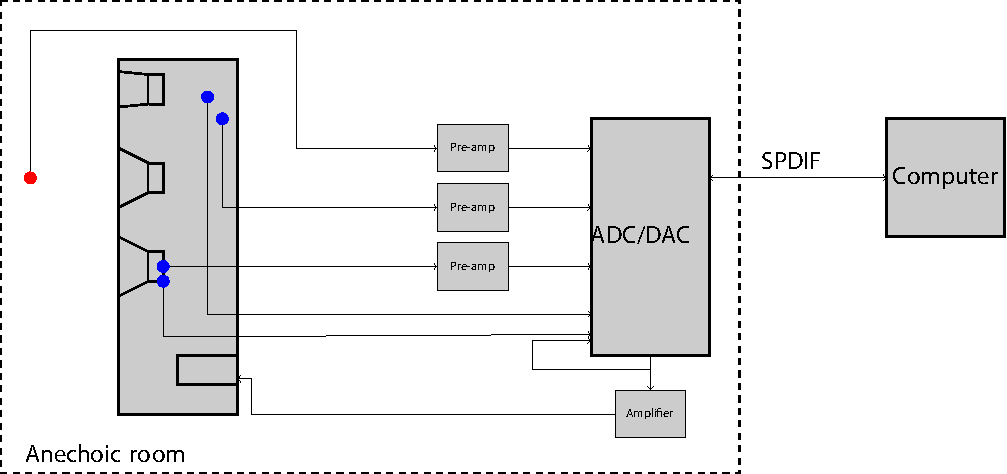
\includegraphics[width=\textwidth]{TestSetup1}
\caption{Test setup}
\label{figure:SpeakertestSetup2}
\end{figure}

\subsection*{Equipment used and AAU-no.}

\begin{table}[H]
\centering
\ra{1.3}
\begin{tabular}{S[table-format=1]ccc} \toprule
    {Item} & {Description} & {AAU-no} \\ \bottomrule 
    1      &  B \& K Accelerometer Type 4319  & 06598   \\ 
    2      &  B \& K Accelerometer Type 4333  & 06596   \\ 
    3      &  B \& K 2-channel Accelerometer Pre-amp Type 2622  & 07013   \\
    4      &  B \& K Microphone Type 4165  & 08132   \\
    5      &  Gras - 26AK Pre-amp & 52665   \\
    6      &  B \& K Microphone Power supply Type 2804  & 07304   \\
    7      &  Crown Studio Reference I Amplifier & 52614   \\
    8      &  BEHRINGER digital A/D \& D/A Converter - Model ADA8000   & 56545   \\
    9      &  B \& K Accelerometer calibrator 4294 & 08023   \\
    10     &  B \& K Microphone calibrator 4231 & 78301   \\
    11     &  RME HammerFall DIGI 96-PDST sound card & 60919  \\
    12     &  TBD Power Supply & 33914  \\
    13     &  ADXL335 Accelerometer (Sparkfun Breakout) & NaN  \\
    14     &  Passive Dali Zensor 5 AX & NaN  \\ \bottomrule 
\end{tabular}
\caption{Table over equipment used in test}
\label{tab:UsedEquipment2}
\end{table}



\section{Procedure}\label{sec:SpeakerTestProcedure2}

The producer for this experiment is described as follows:
\begin{enumerate}
\item Adjust volume on the amplifier to +3 dB gain.
\item Vacate the anechoic room and seal the room.
\item Start recording in Adobe Audition for:
\begin{itemize}
\item Driver and enclosure accelerometers
\item Microphone and playback loop
\end{itemize}
\item Playback file \path{SingleTone.wav}, which is 2 second sinusoidal tone at 50 Hz, then 2 seconds break, then a 2 second sinusoidal tone at 55 Hz which is continued until 100 Hz. The amplitude is 0 dBFS.
\item After playback, stop recording all channels
\item Save recordings as \path{.wav} file
\item Enter room and adjust amplifier by +1 dB
\item Repeat step 2 through 7 13 times.
\end{enumerate}

The \path{SingleTone.wav} can be found on:\\
\scalebox{0.7}{
\path{CD://Maalinger/XX/SingleTone.wav}}\\

\section{Data Extraction}
It was possible to increase the volume by 12 dB before the test was stopped because of the risk of damaging the loudspeaker.
The recordings can be found on:\\
\scalebox{0.7}{
\path{CD://Maalinger/XX}}
And is indexed in folders \scalebox{0.8}{\path{Measure_X}}, where X corresponds to the test number. Every measurements is denoted as:
\begin{itemize}
\item Accelerometer on driver: \scalebox{0.8}{\path{Acc driver_0XX}}
\item Accelerometer in enclosure: \scalebox{0.8}{\path{Acc enclosure_0XX}}
\item Microphone: \scalebox{0.8}{\path{Mic_0XX}}
\item Playback loop: \scalebox{0.8}{\path{Reference_0XX}}
\end{itemize}


\section{Raw data}
For each of the test six measurements was taken. These are the accelerometers placed on the
driver and enclosure, the microphone and a reference to synchronize the measurements.

As previously stated there are in total 13 datasets each containing six measurements. The amount of data is therefore large and only
relevant datasets will be presented. The first dataset from the test is shown in \autoref{fig:raw1t2}.

\begin{figure}[H]
\centering
\begin{subfigure}[t]{0.45\textwidth}
    \centering
    \tikzsetnextfilename{raw_BK_driver1}
    % This file was created by matlab2tikz.
%
%The latest updates can be retrieved from
%  http://www.mathworks.com/matlabcentral/fileexchange/22022-matlab2tikz-matlab2tikz
%where you can also make suggestions and rate matlab2tikz.
%
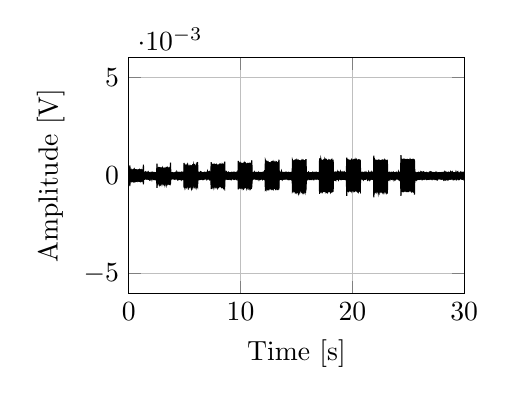
\begin{tikzpicture}

\begin{axis}[%
width=2.3in,
height=1.8in,
at={(0.758in,0.481in)},
xmin=0,
xmax=30,
xmajorgrids,
ymin=-0.006,
ymax=0.006,
ylabel={Amplitude [V]},
xlabel={Time [s]},
ymajorgrids,
axis background/.style={fill=white}
]
\addplot[fill=black,draw=black,forget plot] plot table[row sep=crcr]{%
2.08333333333333e-05	0.000139355659484863\\
0.0252733410493827	0.000130534172058105\\
0.0505258487654321	0.000132203102111816\\
0.0757783564814815	0.00013434886932373\\
0.101030864197531	0.000517368316650391\\
0.12628337191358	0.000305771827697754\\
0.15153587962963	0.000251293182373047\\
0.176788387345679	0.000261306762695313\\
0.202040895061728	0.000280857086181641\\
0.227293402777778	0.000303030014038086\\
0.252545910493827	0.000260353088378906\\
0.277798418209877	0.000263690948486328\\
0.303050925925926	0.000261545181274414\\
0.328303433641975	0.000282406806945801\\
0.353555941358025	0.000287175178527832\\
0.378808449074074	0.000299692153930664\\
0.404060956790123	0.000263810157775879\\
0.429313464506173	0.000283718109130859\\
0.454565972222222	0.000232100486755371\\
0.479818479938272	0.000265359878540039\\
0.505070987654321	0.000320076942443848\\
0.53032349537037	0.000282049179077148\\
0.55557600308642	0.000277996063232422\\
0.580828510802469	0.000287890434265137\\
0.606081018518519	0.00025784969329834\\
0.631333526234568	0.000255823135375977\\
0.656586033950617	0.000295400619506836\\
0.681838541666667	0.000294089317321777\\
0.707091049382716	0.000281691551208496\\
0.732343557098765	0.000273704528808594\\
0.757596064814815	0.000282883644104004\\
0.782848572530864	0.000285863876342773\\
0.808101080246914	0.000280857086181641\\
0.833353587962963	0.000287055969238281\\
0.858606095679012	0.000255346298217773\\
0.883858603395062	0.000286579132080078\\
0.909111111111111	0.000275731086730957\\
0.934363618827161	0.000256180763244629\\
0.95961612654321	0.00025629997253418\\
0.984868634259259	0.000304579734802246\\
1.01012114197531	0.00028538703918457\\
1.03537364969136	0.000283718109130859\\
1.06062615740741	0.000286698341369629\\
1.08587866512346	0.000284194946289063\\
1.11113117283951	0.000301361083984375\\
1.13638368055556	0.000274062156677246\\
1.16163618827161	0.00027155876159668\\
1.18688869598765	0.000272393226623535\\
1.2121412037037	0.000284194946289063\\
1.23739371141975	0.000290036201477051\\
1.2626462191358	0.000284075736999512\\
1.28789872685185	0.000251173973083496\\
1.3131512345679	0.00055992603302002\\
1.33840374228395	0.000141501426696777\\
1.36365625	0.000156164169311523\\
1.38890875771605	0.000165343284606934\\
1.4141612654321	0.00014030933380127\\
1.43941377314815	0.000132322311401367\\
1.4646662808642	0.000142812728881836\\
1.48991878858025	0.000169873237609863\\
1.5151712962963	0.000127315521240234\\
1.54042380401235	0.000159502029418945\\
1.5656763117284	0.00012969970703125\\
1.59092881944444	0.000141143798828125\\
1.61618132716049	0.000160694122314453\\
1.64143383487654	0.000124812126159668\\
1.66668634259259	0.00015723705291748\\
1.69193885030864	0.000117659568786621\\
1.71719135802469	0.000115156173706055\\
1.74244386574074	0.000135660171508789\\
1.76769637345679	0.000171065330505371\\
1.79294888117284	0.000133633613586426\\
1.81820138888889	0.000157713890075684\\
1.84345389660494	0.000153183937072754\\
1.86870640432099	0.00014650821685791\\
1.89395891203704	0.000134706497192383\\
1.91921141975309	0.000138521194458008\\
1.94446392746914	0.000133633613586426\\
1.96971643518519	0.000147223472595215\\
1.99496894290123	0.000168204307556152\\
2.02022145061728	0.000169038772583008\\
2.04547395833333	0.000141024589538574\\
2.07072646604938	0.000141024589538574\\
2.09597897376543	0.000144362449645996\\
2.12123148148148	0.000125527381896973\\
2.14648398919753	0.000167727470397949\\
2.17173649691358	0.00015556812286377\\
2.19698900462963	0.00014650821685791\\
2.22224151234568	0.000155210494995117\\
2.24749402006173	0.000134825706481934\\
2.27274652777778	0.000142216682434082\\
2.29799903549383	0.000142693519592285\\
2.32325154320988	0.000153899192810059\\
2.34850405092593	0.00014650821685791\\
2.37375655864198	0.000136852264404297\\
2.39900906635802	0.000128507614135742\\
2.42426157407407	0.000148892402648926\\
2.44951408179012	0.000157356262207031\\
2.47476658950617	0.000140666961669922\\
2.50001909722222	0.00015556812286377\\
2.52527160493827	0.000600934028625488\\
2.55052411265432	0.00035250186920166\\
2.57577662037037	0.000340938568115234\\
2.60102912808642	0.000369668006896973\\
2.62628163580247	0.000381350517272949\\
2.65153414351852	0.000396490097045898\\
2.67678665123457	0.000332236289978027\\
2.70203915895062	0.000365138053894043\\
2.72729166666667	0.000374197959899902\\
2.75254417438272	0.000403523445129395\\
2.77779668209877	0.000395894050598145\\
2.80304918981481	0.00035560131072998\\
2.82830169753086	0.000330805778503418\\
2.85355420524691	0.000380516052246094\\
2.87880671296296	0.000397562980651855\\
2.90405922067901	0.00038301944732666\\
2.92931172839506	0.000314712524414063\\
2.95456423611111	0.000343441963195801\\
2.97981674382716	0.000372171401977539\\
3.00506925154321	0.000403046607971191\\
3.03032175925926	0.000338315963745117\\
3.05557426697531	0.000355124473571777\\
3.08082677469136	0.000365018844604492\\
3.10607928240741	0.000362992286682129\\
3.13133179012346	0.000374197959899902\\
3.15658429783951	0.000335812568664551\\
3.18183680555556	0.00036919116973877\\
3.2070893132716	0.000369787216186523\\
3.23234182098765	0.000378847122192383\\
3.2575943287037	0.000365853309631348\\
3.28284683641975	0.000346660614013672\\
3.3080993441358	0.000375986099243164\\
3.33335185185185	0.000363826751708984\\
3.3586043595679	0.00040900707244873\\
3.38385686728395	0.000395536422729492\\
3.409109375	0.000338077545166016\\
3.43436188271605	0.000352621078491211\\
3.4596143904321	0.000356793403625488\\
3.48486689814815	0.000413894653320313\\
3.5101194058642	0.000397205352783203\\
3.53537191358025	0.000334620475769043\\
3.5606244212963	0.00036466121673584\\
3.58587692901235	0.000370979309082031\\
3.61112943672839	0.000381708145141602\\
3.63638194444444	0.000337481498718262\\
3.66163445216049	0.000358939170837402\\
3.68688695987654	0.000404834747314453\\
3.71213946759259	0.000386714935302734\\
3.73739197530864	0.000653505325317383\\
3.76264448302469	0.00015103816986084\\
3.78789699074074	0.000159382820129395\\
3.81314949845679	0.000126957893371582\\
3.83840200617284	0.00012814998626709\\
3.86365451388889	0.000142812728881836\\
3.88890702160494	0.000150680541992188\\
3.91415952932099	0.000129461288452148\\
3.93941203703704	0.00013887882232666\\
3.96466454475309	0.000146031379699707\\
3.98991705246914	0.000139832496643066\\
4.01516956018518	0.000128865242004395\\
4.04042206790123	0.000126838684082031\\
4.06567457561728	0.000135540962219238\\
4.09092708333333	0.000140547752380371\\
4.11617959104938	0.000126361846923828\\
4.14143209876543	0.000144362449645996\\
4.16668460648148	0.000162363052368164\\
4.19193711419753	0.00014030933380127\\
4.21718962191358	0.000150203704833984\\
4.24244212962963	0.000135183334350586\\
4.26769463734568	0.000136971473693848\\
4.29294714506173	0.000185370445251465\\
4.31819965277778	0.000134706497192383\\
4.34345216049383	0.00014030933380127\\
4.36870466820988	0.000135660171508789\\
4.39395717592593	0.000122308731079102\\
4.41920968364198	0.000159859657287598\\
4.44446219135802	0.000146389007568359\\
4.46971469907407	0.000140547752380371\\
4.49496720679012	0.000160336494445801\\
4.52021971450617	0.000144362449645996\\
4.54547222222222	0.000151515007019043\\
4.57072472993827	0.000116348266601563\\
4.59597723765432	0.000145554542541504\\
4.62122974537037	0.000120639801025391\\
4.64648225308642	0.000135302543640137\\
4.67173476080247	0.000154495239257813\\
4.69698726851852	0.000166058540344238\\
4.72223977623457	0.00015556812286377\\
4.74749228395062	0.000172734260559082\\
4.77274479166667	0.000146389007568359\\
4.79799729938272	0.000155329704284668\\
4.82324980709877	0.000145196914672852\\
4.84850231481482	0.000167250633239746\\
4.87375482253086	0.0001678466796875\\
4.89900733024691	0.000152349472045898\\
4.92425983796296	0.000154376029968262\\
4.94951234567901	0.000644207000732422\\
4.97476485339506	0.000447273254394531\\
5.00001736111111	0.000517845153808594\\
5.02526986882716	0.000467419624328613\\
5.05052237654321	0.000465750694274902\\
5.07577488425926	0.000495195388793945\\
5.10102739197531	0.000448107719421387\\
5.12627989969136	0.0005035400390625\\
5.15153240740741	0.000437259674072266\\
5.17678491512346	0.000475168228149414\\
5.20203742283951	0.000429272651672363\\
5.22728993055556	0.00047147274017334\\
5.2525424382716	0.00052952766418457\\
5.27779494598765	0.000447630882263184\\
5.3030474537037	0.000513553619384766\\
5.32829996141975	0.00046229362487793\\
5.3535524691358	0.000465154647827148\\
5.37880497685185	0.000473260879516602\\
5.4040574845679	0.000462770462036133\\
5.42930999228395	0.000479459762573242\\
5.4545625	0.000441789627075195\\
5.47981500771605	0.000486016273498535\\
5.5050675154321	0.000441551208496094\\
5.53032002314815	0.000487327575683594\\
5.5555725308642	0.000473618507385254\\
5.58082503858025	0.000464797019958496\\
5.6060775462963	0.00048983097076416\\
5.63133005401235	0.000476956367492676\\
5.65658256172839	0.000449776649475098\\
5.68183506944444	0.000488996505737305\\
5.70708757716049	0.000436782836914063\\
5.73234008487654	0.000490784645080566\\
5.75759259259259	0.000444889068603516\\
5.78284510030864	0.000534534454345703\\
5.80809760802469	0.000415205955505371\\
5.83335011574074	0.000468969345092773\\
5.85860262345679	0.0005035400390625\\
5.88385513117284	0.00043940544128418\\
5.90910763888889	0.000493168830871582\\
5.93436014660494	0.000434756278991699\\
5.95961265432099	0.000480175018310547\\
5.98486516203704	0.000484108924865723\\
6.01011766975309	0.000441908836364746\\
6.03537017746914	0.000519514083862305\\
6.06062268518518	0.000428080558776855\\
6.08587519290123	0.000496029853820801\\
6.11112770061728	0.000446557998657227\\
6.13638020833333	0.000468134880065918\\
6.16163271604938	0.000689268112182617\\
6.18688522376543	0.00014805793762207\\
6.21213773148148	0.000139713287353516\\
6.23739023919753	0.000159740447998047\\
6.26264274691358	0.000131845474243164\\
6.28789525462963	0.00014197826385498\\
6.31314776234568	0.000158071517944336\\
6.33840027006173	0.00016319751739502\\
6.36365277777778	0.000136137008666992\\
6.38890528549383	0.000157713890075684\\
6.41415779320988	0.000181078910827637\\
6.43941030092593	0.000131130218505859\\
6.46466280864198	0.000123143196105957\\
6.48991531635802	0.000166177749633789\\
6.51516782407407	0.000144362449645996\\
6.54042033179012	0.000139355659484863\\
6.56567283950617	0.000149369239807129\\
6.59092534722222	0.000135660171508789\\
6.61617785493827	0.000147700309753418\\
6.64143036265432	0.000144004821777344\\
6.66668287037037	0.000144362449645996\\
6.69193537808642	0.000120162963867188\\
6.71718788580247	0.000143885612487793\\
6.74244039351852	0.00016486644744873\\
6.76769290123457	0.00016319751739502\\
6.79294540895062	0.000169754028320313\\
6.81819791666667	0.000131011009216309\\
6.84345042438272	0.000141143798828125\\
6.86870293209877	0.000154376029968262\\
6.89395543981481	0.000140190124511719\\
6.91920794753086	0.00014805793762207\\
6.94446045524691	0.000153899192810059\\
6.96971296296296	0.000164031982421875\\
6.99496547067901	0.000136494636535645\\
7.02021797839506	0.000147819519042969\\
7.04547048611111	0.000207781791687012\\
7.07072299382716	0.000136017799377441\\
7.09597550154321	0.000126361846923828\\
7.12122800925926	0.000135540962219238\\
7.14648051697531	0.000162720680236816\\
7.17173302469136	0.000125527381896973\\
7.19698553240741	0.000161886215209961\\
7.22223804012346	0.000115513801574707\\
7.24749054783951	0.000171542167663574\\
7.27274305555556	0.000146031379699707\\
7.2979955632716	0.000153183937072754\\
7.32324807098765	0.000164389610290527\\
7.3485005787037	0.00014805793762207\\
7.37375308641975	0.000680208206176758\\
7.3990055941358	0.000515341758728027\\
7.42425810185185	0.000540018081665039\\
7.4495106095679	0.000558257102966309\\
7.47476311728395	0.000528693199157715\\
7.500015625	0.000556588172912598\\
7.52526813271605	0.000568628311157227\\
7.5505206404321	0.000522732734680176\\
7.57577314814815	0.000553607940673828\\
7.6010256558642	0.000545859336853027\\
7.62627816358025	0.000499963760375977\\
7.6515306712963	0.000560760498046875\\
7.67678317901235	0.00053858757019043\\
7.70203568672839	0.000561714172363281\\
7.72728819444444	0.000556111335754395\\
7.75254070216049	0.000483274459838867\\
7.77779320987654	0.000544190406799316\\
7.80304571759259	0.000562429428100586\\
7.82829822530864	0.000520825386047363\\
7.85355073302469	0.000547051429748535\\
7.87880324074074	0.000505805015563965\\
7.90405574845679	0.000531196594238281\\
7.92930825617284	0.000533580780029297\\
7.95456076388889	0.000535011291503906\\
7.97981327160494	0.000542879104614258\\
8.00506577932099	0.000542879104614258\\
8.03031828703704	0.000519514083862305\\
8.05557079475309	0.000533223152160645\\
8.08082330246914	0.000508308410644531\\
8.10607581018519	0.000532865524291992\\
8.13132831790123	0.000562071800231934\\
8.15658082561728	0.000523567199707031\\
8.18183333333333	0.000551104545593262\\
8.20708584104938	0.000518679618835449\\
8.23233834876543	0.000529170036315918\\
8.25759085648148	0.000562787055969238\\
8.28284336419753	0.000500798225402832\\
8.30809587191358	0.000541925430297852\\
8.33334837962963	0.000556111335754395\\
8.35860088734568	0.000520825386047363\\
8.38385339506173	0.000539898872375488\\
8.40910590277778	0.000567913055419922\\
8.43435841049383	0.00047910213470459\\
8.45961091820988	0.000536084175109863\\
8.48486342592593	0.000534415245056152\\
8.51011593364198	0.00054323673248291\\
8.53536844135802	0.000576972961425781\\
8.56062094907407	0.000506162643432617\\
8.58587345679012	0.000706315040588379\\
8.61112596450617	0.000152826309204102\\
8.63637847222222	0.000192046165466309\\
8.66163097993827	0.000131368637084961\\
8.68688348765432	0.000156879425048828\\
8.71213599537037	0.000175356864929199\\
8.73738850308642	0.000132322311401367\\
8.76264101080247	0.000168681144714355\\
8.78789351851852	0.000124335289001465\\
8.81314602623457	0.000156044960021973\\
8.83839853395062	0.000147700309753418\\
8.86365104166667	0.000148892402648926\\
8.88890354938272	0.000146865844726563\\
8.91415605709877	0.000130176544189453\\
8.93940856481481	0.000168204307556152\\
8.96466107253086	0.000144720077514648\\
8.98991358024691	0.000133156776428223\\
9.01516608796296	0.000143527984619141\\
9.04041859567901	0.000147342681884766\\
9.06567110339506	0.000138998031616211\\
9.09092361111111	0.000152230262756348\\
9.11617611882716	0.000145554542541504\\
9.14142862654321	0.000130176544189453\\
9.16668113425926	0.000148892402648926\\
9.19193364197531	0.000166535377502441\\
9.21718614969136	0.000168681144714355\\
9.24243865740741	0.000131964683532715\\
9.26769116512346	0.000132322311401367\\
9.29294367283951	0.00015723705291748\\
9.31819618055556	0.000153541564941406\\
9.34344868827161	0.000143885612487793\\
9.36870119598765	0.000168204307556152\\
9.3939537037037	0.000157356262207031\\
9.41920621141975	0.000143051147460938\\
9.4444587191358	0.00015866756439209\\
9.46971122685185	0.000129342079162598\\
9.4949637345679	0.000125288963317871\\
9.52021624228395	0.00015103816986084\\
9.54546875	0.000128507614135742\\
9.57072125771605	0.000137686729431152\\
9.5959737654321	0.000150322914123535\\
9.62122627314815	0.000152349472045898\\
9.6464787808642	0.000167727470397949\\
9.67173128858025	0.000142693519592285\\
9.6969837962963	0.000161170959472656\\
9.72223630401235	0.000123977661132813\\
9.7474888117284	0.000127792358398438\\
9.77274131944444	0.000148892402648926\\
9.79799382716049	0.000745177268981934\\
9.82324633487654	0.000633358955383301\\
9.84849884259259	0.000583410263061523\\
9.87375135030864	0.000587940216064453\\
9.89900385802469	0.00060427188873291\\
9.92425636574074	0.000611662864685059\\
9.94950887345679	0.000648021697998047\\
9.97476138117284	0.000596165657043457\\
10.0000138888889	0.000609278678894043\\
10.0252663966049	0.000625967979431152\\
10.050518904321	0.00057673454284668\\
10.075771412037	0.00061953067779541\\
10.1010239197531	0.000617623329162598\\
10.1262764274691	0.000620841979980469\\
10.1515289351852	0.000613689422607422\\
10.1767814429012	0.000589489936828613\\
10.2020339506173	0.000583767890930176\\
10.2272864583333	0.000609993934631348\\
10.2525389660494	0.000585079193115234\\
10.2777914737654	0.000609993934631348\\
10.3030439814815	0.000608325004577637\\
10.3282964891975	0.00065302848815918\\
10.3535489969136	0.000605106353759766\\
10.3788015046296	0.000594258308410645\\
10.4040540123457	0.000625848770141602\\
10.4293065200617	0.000580906867980957\\
10.4545590277778	0.000613808631896973\\
10.4798115354938	0.000584125518798828\\
10.5050640432099	0.000595808029174805\\
10.5303165509259	0.000593781471252441\\
10.555569058642	0.000589966773986816\\
10.580821566358	0.000583767890930176\\
10.6060740740741	0.000615477561950684\\
10.6313265817901	0.000605463981628418\\
10.6565790895062	0.000580310821533203\\
10.6818315972222	0.000617027282714844\\
10.7070841049383	0.000621199607849121\\
10.7323366126543	0.000617027282714844\\
10.7575891203704	0.000608325004577637\\
10.7828416280864	0.000574231147766113\\
10.8080941358025	0.000578403472900391\\
10.8333466435185	0.000576138496398926\\
10.8585991512346	0.000630974769592285\\
10.8838516589506	0.000618457794189453\\
10.9091041666667	0.000620841979980469\\
10.9343566743827	0.000612497329711914\\
10.9596091820988	0.000572443008422852\\
10.9848616898148	0.000618815422058105\\
11.0101141975309	0.0007781982421875\\
11.0353667052469	0.000170588493347168\\
11.060619212963	0.000141024589538574\\
11.085871720679	0.000140666961669922\\
11.1111242283951	0.000150680541992188\\
11.1363767361111	0.000151515007019043\\
11.1616292438272	0.000149846076965332\\
11.1868817515432	0.000163555145263672\\
11.2121342592593	0.000146150588989258\\
11.2373867669753	0.000182271003723145\\
11.2626392746914	0.000136852264404297\\
11.2878917824074	0.000156402587890625\\
11.3131442901235	0.000162363052368164\\
11.3383967978395	0.000147342681884766\\
11.3636493055556	0.00012969970703125\\
11.3889018132716	0.000122785568237305\\
11.4141543209877	0.000154495239257813\\
11.4394068287037	0.000137805938720703\\
11.4646593364198	0.00013267993927002\\
11.4899118441358	0.000128030776977539\\
11.5151643518519	0.000145554542541504\\
11.5404168595679	0.000158071517944336\\
11.565669367284	0.000148177146911621\\
11.590921875	0.000144720077514648\\
11.6161743827161	0.000168919563293457\\
11.6414268904321	0.000129461288452148\\
11.6666793981481	0.000144362449645996\\
11.6919319058642	0.00012516975402832\\
11.7171844135802	0.000140666961669922\\
11.7424369212963	0.000145673751831055\\
11.7676894290123	0.000136137008666992\\
11.7929419367284	0.000150680541992188\\
11.8181944444444	0.000144362449645996\\
11.8434469521605	0.000157713890075684\\
11.8686994598765	0.000154376029968262\\
11.8939519675926	0.000146031379699707\\
11.9192044753086	0.000146865844726563\\
11.9444569830247	0.000145673751831055\\
11.9697094907407	0.000158548355102539\\
11.9949619984568	0.000132322311401367\\
12.0202145061728	0.000149846076965332\\
12.0454670138889	0.000126481056213379\\
12.0707195216049	0.000160574913024902\\
12.095972029321	0.000147700309753418\\
12.121224537037	0.000191211700439453\\
12.1464770447531	0.00015103816986084\\
12.1717295524691	0.000116348266601563\\
12.1969820601852	0.000146985054016113\\
12.2222345679012	0.000785231590270996\\
12.2474870756173	0.000746011734008789\\
12.2727395833333	0.000680208206176758\\
12.2979920910494	0.000633478164672852\\
12.3232445987654	0.000703573226928711\\
12.3484971064815	0.000678896903991699\\
12.3737496141975	0.000694632530212402\\
12.3990021219136	0.00065767765045166\\
12.4242546296296	0.000658392906188965\\
12.4495071373457	0.000644564628601074\\
12.4747596450617	0.000694632530212402\\
12.5000121527778	0.000671029090881348\\
12.5252646604938	0.000652909278869629\\
12.5505171682099	0.000644564628601074\\
12.5757696759259	0.000646829605102539\\
12.601022183642	0.000655174255371094\\
12.626274691358	0.000642180442810059\\
12.6515271990741	0.000647664070129395\\
12.6767797067901	0.000645995140075684\\
12.7020322145062	0.000657558441162109\\
12.7272847222222	0.000676870346069336\\
12.7525372299383	0.000662922859191895\\
12.7777897376543	0.000686407089233398\\
12.8030422453704	0.000659704208374023\\
12.8282947530864	0.000690937042236328\\
12.8535472608025	0.000655412673950195\\
12.8787997685185	0.000686287879943848\\
12.9040522762346	0.000656247138977051\\
12.9293047839506	0.000633716583251953\\
12.9545572916667	0.000643014907836914\\
12.9798097993827	0.00069892406463623\\
13.0050623070988	0.000648021697998047\\
13.0303148148148	0.00068056583404541\\
13.0555673225309	0.000663399696350098\\
13.0808198302469	0.000636816024780273\\
13.106072337963	0.000639557838439941\\
13.131324845679	0.00066375732421875\\
13.1565773533951	0.000692605972290039\\
13.1818298611111	0.000665068626403809\\
13.2070823688272	0.00067436695098877\\
13.2323348765432	0.000688552856445313\\
13.2575873842593	0.000659346580505371\\
13.2828398919753	0.000650405883789063\\
13.3080923996914	0.000657081604003906\\
13.3333449074074	0.000650167465209961\\
13.3585974151235	0.000650167465209961\\
13.3838499228395	0.000656366348266602\\
13.4091024305556	0.000648021697998047\\
13.4343549382716	0.000808954238891602\\
13.4596074459877	0.000192403793334961\\
13.4848599537037	0.000163078308105469\\
13.5101124614198	0.00017857551574707\\
13.5353649691358	0.000149846076965332\\
13.5606174768519	0.000126838684082031\\
13.5858699845679	0.000129818916320801\\
13.611122492284	0.000122308731079102\\
13.636375	0.000138640403747559\\
13.6616275077161	0.000224113464355469\\
13.6868800154321	0.000174880027770996\\
13.7121325231481	0.00016486644744873\\
13.7373850308642	0.000156879425048828\\
13.7626375385802	0.000142812728881836\\
13.7878900462963	0.000155329704284668\\
13.8131425540123	0.00015866756439209\\
13.8383950617284	0.000148653984069824\\
13.8636475694444	0.00013887882232666\\
13.8889000771605	0.000149846076965332\\
13.9141525848765	0.000141143798828125\\
13.9394050925926	0.00015866756439209\\
13.9646576003086	0.000160574913024902\\
13.9899101080247	0.000110149383544922\\
14.0151626157407	0.000136971473693848\\
14.0404151234568	0.000170230865478516\\
14.0656676311728	0.000179052352905273\\
14.0909201388889	0.000151515007019043\\
14.1161726466049	0.000145673751831055\\
14.141425154321	0.000143170356750488\\
14.166677662037	0.000152707099914551\\
14.1919301697531	0.000142216682434082\\
14.2171826774691	0.000148177146911621\\
14.2424351851852	0.000141143798828125\\
14.2676876929012	0.000159740447998047\\
14.2929402006173	0.00016939640045166\\
14.3181927083333	0.000171422958374023\\
14.3434452160494	0.000132322311401367\\
14.3686977237654	0.000140666961669922\\
14.3939502314815	0.000140547752380371\\
14.4192027391975	0.000147342681884766\\
14.4444552469136	0.000153183937072754\\
14.4697077546296	0.000154018402099609\\
14.4949602623457	0.000146865844726563\\
14.5202127700617	0.000119447708129883\\
14.5454652777778	0.00014030933380127\\
14.5707177854938	0.000163078308105469\\
14.5959702932099	0.000136971473693848\\
14.6212228009259	0.000152826309204102\\
14.646475308642	0.000785231590270996\\
14.671727816358	0.000745654106140137\\
14.6969803240741	0.000751137733459473\\
14.7222328317901	0.000748038291931152\\
14.7474853395062	0.000739336013793945\\
14.7727378472222	0.000737786293029785\\
14.7979903549383	0.000749468803405762\\
14.8232428626543	0.000768661499023438\\
14.8484953703704	0.000745296478271484\\
14.8737478780864	0.000713586807250977\\
14.8990003858025	0.000762224197387695\\
14.9242528935185	0.00078272819519043\\
14.9495054012346	0.000728845596313477\\
14.9747579089506	0.00074613094329834\\
15.0000104166667	0.000715494155883789\\
15.0252629243827	0.000785708427429199\\
15.0505154320988	0.000753521919250488\\
15.0757679398148	0.000752806663513184\\
15.1010204475309	0.000724434852600098\\
15.1262729552469	0.000715136528015137\\
15.151525462963	0.000786423683166504\\
15.176777970679	0.000762701034545898\\
15.2020304783951	0.000743985176086426\\
15.2272829861111	0.000748872756958008\\
15.2525354938272	0.000751852989196777\\
15.2777880015432	0.000754714012145996\\
15.3030405092593	0.000740289688110352\\
15.3282930169753	0.000740170478820801\\
15.3535455246914	0.000707268714904785\\
15.3787980324074	0.000744819641113281\\
15.4040505401235	0.00075685977935791\\
15.4293030478395	0.000711441040039063\\
15.4545555555556	0.000747799873352051\\
15.4798080632716	0.000730514526367188\\
15.5050605709877	0.000779390335083008\\
15.5303130787037	0.000745296478271484\\
15.5555655864198	0.000719308853149414\\
15.5808180941358	0.000759720802307129\\
15.6060706018519	0.000744462013244629\\
15.6313231095679	0.000765562057495117\\
15.656575617284	0.000711798667907715\\
15.681828125	0.000737786293029785\\
15.7070806327161	0.000755548477172852\\
15.7323331404321	0.000751376152038574\\
15.7575856481481	0.000752687454223633\\
15.7828381558642	0.000724673271179199\\
15.8080906635802	0.000763058662414551\\
15.8333431712963	0.000746488571166992\\
15.8585956790123	0.000834822654724121\\
15.8838481867284	0.000151991844177246\\
15.9091006944444	0.000148177146911621\\
15.9343532021605	0.000142693519592285\\
15.9596057098765	0.00014185905456543\\
15.9848582175926	0.000128507614135742\\
16.0101107253086	0.000145196914672852\\
16.0353632330247	0.000134468078613281\\
16.0606157407407	0.000159740447998047\\
16.0858682484568	0.000184059143066406\\
16.1111207561728	0.000161886215209961\\
16.1363732638889	0.00013887882232666\\
16.1616257716049	0.000122785568237305\\
16.186878279321	0.0001373291015625\\
16.212130787037	0.000142693519592285\\
16.2373832947531	0.000139355659484863\\
16.2626358024691	0.000142693519592285\\
16.2878883101852	0.000131130218505859\\
16.3131408179012	0.00014805793762207\\
16.3383933256173	0.000143051147460938\\
16.3636458333333	0.00014805793762207\\
16.3888983410494	0.000142693519592285\\
16.4141508487654	0.000148653984069824\\
16.4394033564815	0.000165700912475586\\
16.4646558641975	0.000133514404296875\\
16.4899083719136	0.000142693519592285\\
16.5151608796296	0.000138521194458008\\
16.5404133873457	0.000154376029968262\\
16.5656658950617	0.000163912773132324\\
16.5909184027778	0.000152707099914551\\
16.6161709104938	0.000130534172058105\\
16.6414234182099	0.000154733657836914\\
16.6666759259259	0.000146865844726563\\
16.691928433642	0.000152349472045898\\
16.717180941358	0.000154018402099609\\
16.7424334490741	0.00016939640045166\\
16.7676859567901	0.00016939640045166\\
16.7929384645062	0.000171065330505371\\
16.8181909722222	0.000133872032165527\\
16.8434434799383	0.000139474868774414\\
16.8686959876543	0.00015103816986084\\
16.8939484953704	0.000152230262756348\\
16.9192010030864	0.000145316123962402\\
16.9444535108025	0.00014650821685791\\
16.9697060185185	0.000154018402099609\\
16.9949585262346	0.000144362449645996\\
17.0202110339506	0.000146865844726563\\
17.0454635416667	0.000151872634887695\\
17.0707160493827	0.000879049301147461\\
17.0959685570988	0.000776171684265137\\
17.1212210648148	0.00071108341217041\\
17.1464735725309	0.000751495361328125\\
17.1717260802469	0.000856637954711914\\
17.196978587963	0.000767230987548828\\
17.222231095679	0.000791192054748535\\
17.2474836033951	0.00077521800994873\\
17.2727361111111	0.000768542289733887\\
17.2979886188272	0.000770211219787598\\
17.3232411265432	0.000754833221435547\\
17.3484936342593	0.00075221061706543\\
17.3737461419753	0.000770330429077148\\
17.3989986496914	0.000753641128540039\\
17.4242511574074	0.000784873962402344\\
17.4495036651235	0.000758171081542969\\
17.4747561728395	0.000751495361328125\\
17.5000086805556	0.000749349594116211\\
17.5252611882716	0.000820636749267578\\
17.5505136959877	0.000747203826904297\\
17.5757662037037	0.000777244567871094\\
17.6010187114198	0.00075685977935791\\
17.6262712191358	0.000801920890808105\\
17.6515237268519	0.000771522521972656\\
17.6767762345679	0.000743865966796875\\
17.702028742284	0.000784039497375488\\
17.72728125	0.000749826431274414\\
17.7525337577161	0.000774741172790527\\
17.7777862654321	0.000774502754211426\\
17.8030387731481	0.000760316848754883\\
17.8282912808642	0.000776529312133789\\
17.8535437885803	0.000778913497924805\\
17.8787962962963	0.00075531005859375\\
17.9040488040123	0.000795722007751465\\
17.9293013117284	0.000775337219238281\\
17.9545538194444	0.00079035758972168\\
17.9798063271605	0.000781059265136719\\
18.0050588348765	0.000723600387573242\\
18.0303113425926	0.000777244567871094\\
18.0555638503086	0.000778675079345703\\
18.0808163580247	0.000784873962402344\\
18.1060688657407	0.000791549682617188\\
18.1313213734568	0.00080573558807373\\
18.1565738811728	0.000746488571166992\\
18.1818263888889	0.000791430473327637\\
18.2070788966049	0.000731110572814941\\
18.232331404321	0.000749707221984863\\
18.257583912037	0.000773072242736816\\
18.2828364197531	0.000777244567871094\\
18.3080889274691	0.000192046165466309\\
18.3333414351852	0.00014030933380127\\
18.3585939429012	0.000141501426696777\\
18.3838464506173	0.000163078308105469\\
18.4090989583333	0.000169038772583008\\
18.4343514660494	0.000145673751831055\\
18.4596039737654	0.000146985054016113\\
18.4848564814815	0.000172853469848633\\
18.5101089891975	0.000182747840881348\\
18.5353614969136	0.000183939933776855\\
18.5606140046296	0.000175595283508301\\
18.5858665123457	0.000153660774230957\\
18.6111190200617	0.000138640403747559\\
18.6363715277778	0.000133633613586426\\
18.6616240354938	0.000153183937072754\\
18.6868765432099	0.000198245048522949\\
18.7121290509259	0.000141024589538574\\
18.737381558642	0.000131130218505859\\
18.762634066358	0.000162720680236816\\
18.7878865740741	0.000182271003723145\\
18.8131390817901	0.000155210494995117\\
18.8383915895062	0.000164031982421875\\
18.8636440972222	0.000131964683532715\\
18.8888966049383	0.000152230262756348\\
18.9141491126543	0.000123858451843262\\
18.9394016203704	0.000193119049072266\\
18.9646541280864	0.000136852264404297\\
18.9899066358025	0.000149369239807129\\
19.0151591435185	0.000141143798828125\\
19.0404116512346	0.000151157379150391\\
19.0656641589506	0.000174403190612793\\
19.0909166666667	0.000159502029418945\\
19.1161691743827	0.000143647193908691\\
19.1414216820988	0.000148534774780273\\
19.1666741898148	0.000181913375854492\\
19.1919266975309	0.000153660774230957\\
19.2171792052469	0.000141143798828125\\
19.242431712963	0.0001373291015625\\
19.267684220679	0.000140190124511719\\
19.2929367283951	0.000171065330505371\\
19.3181892361111	0.000127673149108887\\
19.3434417438272	0.000150322914123535\\
19.3686942515432	0.000133991241455078\\
19.3939467592593	0.000150680541992188\\
19.4191992669753	0.000150203704833984\\
19.4444517746914	0.000157356262207031\\
19.4697042824074	0.000133633613586426\\
19.4949567901235	0.000909924507141113\\
19.5202092978395	0.000756144523620605\\
19.5454618055556	0.000767230987548828\\
19.5707143132716	0.000761032104492188\\
19.5959668209877	0.000788092613220215\\
19.6212193287037	0.000724673271179199\\
19.6464718364198	0.00076603889465332\\
19.6717243441358	0.000758647918701172\\
19.6969768518519	0.000789403915405273\\
19.7222293595679	0.000785231590270996\\
19.747481867284	0.000743865966796875\\
19.772734375	0.000749468803405762\\
19.797986882716	0.000751137733459473\\
19.8232393904321	0.000763177871704102\\
19.8484918981482	0.00075531005859375\\
19.8737444058642	0.000748872756958008\\
19.8989969135802	0.000785708427429199\\
19.9242494212963	0.000746488571166992\\
19.9495019290123	0.000786423683166504\\
19.9747544367284	0.000728607177734375\\
20.0000069444444	0.000787854194641113\\
20.0252594521605	0.000778555870056152\\
20.0505119598765	0.000747799873352051\\
20.0757644675926	0.000779867172241211\\
20.1010169753086	0.000748157501220703\\
20.1262694830247	0.000764846801757813\\
20.1515219907407	0.000794887542724609\\
20.1767744984568	0.000763654708862305\\
20.2020270061728	0.00076138973236084\\
20.2272795138889	0.000749349594116211\\
20.2525320216049	0.000811457633972168\\
20.277784529321	0.000759005546569824\\
20.303037037037	0.000782012939453125\\
20.3282895447531	0.000760197639465332\\
20.3535420524691	0.00072944164276123\\
20.3787945601852	0.000793933868408203\\
20.4040470679012	0.000755548477172852\\
20.4292995756173	0.000771045684814453\\
20.4545520833333	0.000781536102294922\\
20.4798045910494	0.000786185264587402\\
20.5050570987654	0.000760674476623535\\
20.5303096064815	0.000755667686462402\\
20.5555621141975	0.000784516334533691\\
20.5808146219136	0.000750541687011719\\
20.6060671296296	0.000754833221435547\\
20.6313196373457	0.000771999359130859\\
20.6565721450617	0.000732183456420898\\
20.6818246527778	0.000782012939453125\\
20.7070771604938	0.00075685977935791\\
20.7323296682099	0.000182747840881348\\
20.7575821759259	0.000161051750183105\\
20.782834683642	0.000133037567138672\\
20.808087191358	0.000137209892272949\\
20.8333396990741	0.000151157379150391\\
20.8585922067901	0.000139832496643066\\
20.8838447145062	0.000167369842529297\\
20.9090972222222	0.000156521797180176\\
20.9343497299383	0.000160574913024902\\
20.9596022376543	0.000151157379150391\\
20.9848547453704	0.000123858451843262\\
21.0101072530864	0.00015556812286377\\
21.0353597608025	0.000152349472045898\\
21.0606122685185	0.000151395797729492\\
21.0858647762346	0.000166416168212891\\
21.1111172839506	0.000135302543640137\\
21.1363697916667	0.000118494033813477\\
21.1616222993827	0.00013887882232666\\
21.1868748070988	0.000147819519042969\\
21.2121273148148	0.000178098678588867\\
21.2373798225309	0.000138998031616211\\
21.2626323302469	0.000158071517944336\\
21.287884837963	0.000154018402099609\\
21.313137345679	0.000143051147460938\\
21.3383898533951	0.000143051147460938\\
21.3636423611111	0.000136375427246094\\
21.3888948688272	0.000130295753479004\\
21.4141473765432	0.000128626823425293\\
21.4393998842593	0.000121951103210449\\
21.4646523919753	0.00019228458404541\\
21.4899048996914	0.000156402587890625\\
21.5151574074074	0.000151872634887695\\
21.5404099151235	0.000129818916320801\\
21.5656624228395	0.000122189521789551\\
21.5909149305556	0.000143170356750488\\
21.6161674382716	0.000170707702636719\\
21.6414199459877	0.000165581703186035\\
21.6666724537037	0.000134825706481934\\
21.6919249614198	0.000157356262207031\\
21.7171774691358	0.000123500823974609\\
21.7424299768519	0.000173211097717285\\
21.7676824845679	0.000131845474243164\\
21.792934992284	0.000133037567138672\\
21.8181875	0.000131130218505859\\
21.8434400077161	0.000152707099914551\\
21.8686925154321	0.000160574913024902\\
21.8939450231481	0.000162720680236816\\
21.9191975308642	0.00101423263549805\\
21.9444500385803	0.000726938247680664\\
21.9697025462963	0.000751137733459473\\
21.9949550540123	0.000807285308837891\\
22.0202075617284	0.000760674476623535\\
22.0454600694444	0.000769495964050293\\
22.0707125771605	0.000720977783203125\\
22.0959650848765	0.000784754753112793\\
22.1212175925926	0.000783562660217285\\
22.1464701003086	0.000765562057495117\\
22.1717226080247	0.000745534896850586\\
22.1969751157407	0.00072026252746582\\
22.2222276234568	0.000770211219787598\\
22.2474801311728	0.000768661499023438\\
22.2727326388889	0.00077366828918457\\
22.2979851466049	0.000736117362976074\\
22.323237654321	0.000733017921447754\\
22.348490162037	0.000776410102844238\\
22.3737426697531	0.000758528709411621\\
22.3989951774691	0.000770330429077148\\
22.4242476851852	0.000738859176635742\\
22.4495001929012	0.000724673271179199\\
22.4747527006173	0.000765681266784668\\
22.5000052083333	0.000754714012145996\\
22.5252577160494	0.000759363174438477\\
22.5505102237654	0.000740528106689453\\
22.5757627314815	0.000765323638916016\\
22.6010152391975	0.000777721405029297\\
22.6262677469136	0.00075984001159668\\
22.6515202546296	0.000753879547119141\\
22.6767727623457	0.000735282897949219\\
22.7020252700617	0.000788211822509766\\
22.7272777777778	0.000779867172241211\\
22.7525302854938	0.000775575637817383\\
22.7777827932099	0.000717759132385254\\
22.8030353009259	0.000732779502868652\\
22.828287808642	0.000770330429077148\\
22.853540316358	0.000798702239990234\\
22.8787928240741	0.000738978385925293\\
22.9040453317901	0.000734806060791016\\
22.9292978395062	0.000717759132385254\\
22.9545503472222	0.000786900520324707\\
22.9798028549383	0.000780582427978516\\
23.0050553626543	0.000756382942199707\\
23.0303078703704	0.000748157501220703\\
23.0555603780864	0.00075232982635498\\
23.0808128858025	0.000764727592468262\\
23.1060653935185	0.000779509544372559\\
23.1313179012346	0.000746965408325195\\
23.1565704089506	0.000177264213562012\\
23.1818229166667	0.000172257423400879\\
23.2070754243827	0.000144004821777344\\
23.2323279320988	0.000138163566589355\\
23.2575804398148	0.00014185905456543\\
23.2828329475309	0.000141143798828125\\
23.3080854552469	0.000162243843078613\\
23.333337962963	0.000138521194458008\\
23.358590470679	0.000137805938720703\\
23.3838429783951	0.000130653381347656\\
23.4090954861111	0.000139474868774414\\
23.4343479938272	0.000144004821777344\\
23.4596005015432	0.000163674354553223\\
23.4848530092593	0.000133633613586426\\
23.5101055169753	0.000143885612487793\\
23.5353580246914	0.000135302543640137\\
23.5606105324074	0.000153183937072754\\
23.5858630401235	0.000144362449645996\\
23.6111155478395	0.000152826309204102\\
23.6363680555556	0.000155329704284668\\
23.6616205632716	0.000169754028320313\\
23.6868730709877	0.000134468078613281\\
23.7121255787037	0.000123977661132813\\
23.7373780864198	0.000137209892272949\\
23.7626305941358	0.000145316123962402\\
23.7878831018519	0.000154376029968262\\
23.8131356095679	0.00015568733215332\\
23.838388117284	0.000142812728881836\\
23.863640625	0.000153183937072754\\
23.888893132716	0.000133633613586426\\
23.9141456404321	0.000142216682434082\\
23.9393981481482	0.000164508819580078\\
23.9646506558642	0.000139355659484863\\
23.9899031635802	0.000134468078613281\\
24.0151556712963	0.000127196311950684\\
24.0404081790123	0.000118851661682129\\
24.0656606867284	0.000126481056213379\\
24.0909131944444	0.000147342681884766\\
24.1161657021605	0.000202417373657227\\
24.1414182098765	0.000150680541992188\\
24.1666707175926	0.000131487846374512\\
24.1919232253086	0.000143647193908691\\
24.2171757330247	0.000131964683532715\\
24.2424282407407	0.000143527984619141\\
24.2676807484568	0.000171422958374023\\
24.2929332561728	0.000122785568237305\\
24.3181857638889	0.000139355659484863\\
24.3434382716049	0.00104153156280518\\
24.368690779321	0.00081789493560791\\
24.393943287037	0.000803112983703613\\
24.4191957947531	0.000796198844909668\\
24.4444483024691	0.000827312469482422\\
24.4697008101852	0.000821471214294434\\
24.4949533179012	0.00082242488861084\\
24.5202058256173	0.000780582427978516\\
24.5454583333333	0.000809907913208008\\
24.5707108410494	0.000770330429077148\\
24.5959633487654	0.00080406665802002\\
24.6212158564815	0.000822782516479492\\
24.6464683641975	0.000768899917602539\\
24.6717208719136	0.000779390335083008\\
24.6969733796296	0.00080108642578125\\
24.7222258873457	0.000810742378234863\\
24.7474783950617	0.000783681869506836\\
24.7727309027778	0.000790596008300781\\
24.7979834104938	0.000784873962402344\\
24.8232359182099	0.000818252563476563\\
24.8484884259259	0.000812292098999023\\
24.873740933642	0.00078284740447998\\
24.898993441358	0.000792264938354492\\
24.9242459490741	0.000815749168395996\\
24.9494984567901	0.000794887542724609\\
24.9747509645062	0.000808238983154297\\
25.0000034722222	0.000809788703918457\\
25.0252559799383	0.000808119773864746\\
25.0505084876543	0.000784873962402344\\
25.0757609953704	0.000781536102294922\\
25.1010135030864	0.000779867172241211\\
25.1262660108025	0.000794053077697754\\
25.1515185185185	0.000830769538879395\\
25.1767710262346	0.000781893730163574\\
25.2020235339506	0.000793933868408203\\
25.2272760416667	0.0008087158203125\\
25.2525285493827	0.00078117847442627\\
25.2777810570988	0.000792860984802246\\
25.3030335648148	0.000806093215942383\\
25.3282860725309	0.000807285308837891\\
25.3535385802469	0.000774741172790527\\
25.378791087963	0.000780344009399414\\
25.404043595679	0.000826120376586914\\
25.4292961033951	0.000821471214294434\\
25.4545486111111	0.000807046890258789\\
25.4798011188272	0.000790238380432129\\
25.5050536265432	0.000817298889160156\\
25.5303061342593	0.000802278518676758\\
25.5555586419753	0.000745296478271484\\
25.5808111496914	0.000197887420654297\\
25.6060636574074	0.000167727470397949\\
25.6313161651235	0.000171542167663574\\
25.6565686728395	0.00014197826385498\\
25.6818211805556	0.000135302543640137\\
25.7070736882716	0.000118613243103027\\
25.7323261959877	0.000126838684082031\\
25.7575787037037	0.000152230262756348\\
25.7828312114198	0.000154852867126465\\
25.8080837191358	0.000151991844177246\\
25.8333362268519	0.000143527984619141\\
25.8585887345679	0.000135540962219238\\
25.883841242284	0.000143051147460938\\
25.90909375	0.000159025192260742\\
25.9343462577161	0.000134825706481934\\
25.9595987654321	0.000160694122314453\\
25.9848512731481	0.00014197826385498\\
26.0101037808642	0.000136375427246094\\
26.0353562885803	0.000139713287353516\\
26.0606087962963	0.000147223472595215\\
26.0858613040123	0.000154733657836914\\
26.1111138117284	0.00018310546875\\
26.1363663194444	0.000123500823974609\\
26.1616188271605	0.000131130218505859\\
26.1868713348765	0.000156879425048828\\
26.2121238425926	0.000120997428894043\\
26.2373763503086	0.000156998634338379\\
26.2626288580247	0.000140547752380371\\
26.2878813657407	0.000138998031616211\\
26.3131338734568	0.00016939640045166\\
26.3383863811728	0.000142216682434082\\
26.3636388888889	0.000170707702636719\\
26.3888913966049	0.000137686729431152\\
26.414143904321	0.000149011611938477\\
26.439396412037	0.000159025192260742\\
26.4646489197531	0.000133514404296875\\
26.4899014274691	0.000141024589538574\\
26.5151539351852	0.000138044357299805\\
26.5404064429012	0.000149846076965332\\
26.5656589506173	0.000139713287353516\\
26.5909114583333	0.000138044357299805\\
26.6161639660494	0.00015556812286377\\
26.6414164737654	0.000138640403747559\\
26.6666689814815	0.00015723705291748\\
26.6919214891975	0.000149011611938477\\
26.7171739969136	0.000141143798828125\\
26.7424265046296	0.000130534172058105\\
26.7676790123457	0.000136137008666992\\
26.7929315200617	0.000126481056213379\\
26.8181840277778	0.000128626823425293\\
26.8434365354938	0.000145673751831055\\
26.8686890432099	0.000167250633239746\\
26.8939415509259	0.000141382217407227\\
26.919194058642	0.00014197826385498\\
26.944446566358	0.000164031982421875\\
26.9696990740741	0.000143051147460938\\
26.9949515817901	0.000175237655639648\\
27.0202040895062	0.000143885612487793\\
27.0454565972222	0.000138640403747559\\
27.0707091049383	0.000128030776977539\\
27.0959616126543	0.000165700912475586\\
27.1212141203704	0.000146150588989258\\
27.1464666280864	0.00014805793762207\\
27.1717191358025	0.000143885612487793\\
27.1969716435185	0.000158548355102539\\
27.2222241512346	0.000153541564941406\\
27.2474766589506	0.000156879425048828\\
27.2727291666667	0.000149846076965332\\
27.2979816743827	0.000138521194458008\\
27.3232341820988	0.00014805793762207\\
27.3484866898148	0.000154852867126465\\
27.3737391975309	0.000150322914123535\\
27.3989917052469	0.000118136405944824\\
27.424244212963	0.000141501426696777\\
27.449496720679	0.000132203102111816\\
27.4747492283951	0.000169515609741211\\
27.5000017361111	0.000143647193908691\\
27.5252542438272	0.000126361846923828\\
27.5505067515432	0.000133872032165527\\
27.5757592592593	0.000155329704284668\\
27.6010117669753	0.000136017799377441\\
27.6262642746914	0.000124692916870117\\
27.6515167824074	0.000118136405944824\\
27.6767692901235	0.000136494636535645\\
27.7020217978395	0.000147342681884766\\
27.7272743055556	0.00014185905456543\\
27.7525268132716	0.000151515007019043\\
27.7777793209877	0.000145316123962402\\
27.8030318287037	0.000149846076965332\\
27.8282843364198	0.000138044357299805\\
27.8535368441358	0.000141024589538574\\
27.8787893518519	0.000139474868774414\\
27.9040418595679	0.000148534774780273\\
27.929294367284	0.000154852867126465\\
27.954546875	0.000147819519042969\\
27.979799382716	0.00012052059173584\\
28.0050518904321	0.000146150588989258\\
28.0303043981482	0.000137686729431152\\
28.0555569058642	0.00015556812286377\\
28.0808094135802	0.000159502029418945\\
28.1060619212963	0.000145554542541504\\
28.1313144290123	0.000120997428894043\\
28.1565669367284	0.000146985054016113\\
28.1818194444444	0.000136137008666992\\
28.2070719521605	0.000138044357299805\\
28.2323244598765	0.000181436538696289\\
28.2575769675926	0.000140547752380371\\
28.2828294753086	0.00014948844909668\\
28.3080819830247	0.000175714492797852\\
28.3333344907407	0.000151157379150391\\
28.3585869984568	0.000168681144714355\\
28.3838395061728	0.000160574913024902\\
28.4090920138889	0.000142216682434082\\
28.4343445216049	0.00016474723815918\\
28.459597029321	0.000157833099365234\\
28.484849537037	0.00015556812286377\\
28.5101020447531	0.000143527984619141\\
28.5353545524691	0.000165343284606934\\
28.5606070601852	0.000165700912475586\\
28.5858595679012	0.000121831893920898\\
28.6111120756173	0.000151515007019043\\
28.6363645833333	0.000125288963317871\\
28.6616170910494	0.000157833099365234\\
28.6868695987654	0.000147342681884766\\
28.7121221064815	0.000149011611938477\\
28.7373746141975	0.000138998031616211\\
28.7626271219136	0.00012969970703125\\
28.7878796296296	0.000185251235961914\\
28.8131321373457	0.000151395797729492\\
28.8383846450617	0.000141024589538574\\
28.8636371527778	0.0001373291015625\\
28.8888896604938	0.000171065330505371\\
28.9141421682099	0.00015556812286377\\
28.9393946759259	0.00015723705291748\\
28.964647183642	0.000182271003723145\\
28.989899691358	0.000122308731079102\\
29.0151521990741	0.000145316123962402\\
29.0404047067901	0.000149011611938477\\
29.0656572145062	0.000150203704833984\\
29.0909097222222	0.000150561332702637\\
29.1161622299383	0.000139832496643066\\
29.1414147376543	0.000148653984069824\\
29.1666672453704	0.000137805938720703\\
29.1919197530864	0.000141143798828125\\
29.2171722608025	0.000133156776428223\\
29.2424247685185	0.000131964683532715\\
29.2676772762346	0.000191092491149902\\
29.2929297839506	0.000148177146911621\\
29.3181822916667	0.000136494636535645\\
29.3434347993827	0.000154376029968262\\
29.3686873070988	0.000147223472595215\\
29.3939398148148	0.000168919563293457\\
29.4191923225309	0.000134706497192383\\
29.4444448302469	0.000172019004821777\\
29.469697337963	0.000116348266601563\\
29.494949845679	0.000131011009216309\\
29.5202023533951	0.000130176544189453\\
29.5454548611111	0.000136494636535645\\
29.5707073688272	0.000133872032165527\\
29.5959598765432	0.000138521194458008\\
29.6212123842593	0.000140666961669922\\
29.6464648919753	0.000168204307556152\\
29.6717173996914	0.000161528587341309\\
29.6969699074074	0.000180721282958984\\
29.7222224151235	0.000141382217407227\\
29.7474749228395	0.000143527984619141\\
29.7727274305556	0.000130653381347656\\
29.7979799382716	0.000152707099914551\\
29.8232324459877	0.000148892402648926\\
29.8484849537037	0.000134825706481934\\
29.8737374614198	0.000128865242004395\\
29.8989899691358	0.000175237655639648\\
29.9242424768519	0.000167250633239746\\
29.9494949845679	0.00013887882232666\\
29.9747474922839	0.000149011611938477\\
30	0.000145316123962402\\
}
\closedcycle;
\addplot[fill=black,draw=black,forget plot] plot table[row sep=crcr]{%
2.08333333333333e-05	-0.000190138816833496\\
0.0252733410493827	-0.000181436538696289\\
0.0505258487654321	-0.000171542167663574\\
0.0757783564814815	-0.000167369842529297\\
0.101030864197531	-0.000539779663085938\\
0.12628337191358	-0.00028836727142334\\
0.15153587962963	-0.000279903411865234\\
0.176788387345679	-0.000267744064331055\\
0.202040895061728	-0.000289440155029297\\
0.227293402777778	-0.000267386436462402\\
0.252545910493827	-0.000266194343566895\\
0.277798418209877	-0.000306248664855957\\
0.303050925925926	-0.000291228294372559\\
0.328303433641975	-0.000272512435913086\\
0.353555941358025	-0.000284194946289063\\
0.378808449074074	-0.000274181365966797\\
0.404060956790123	-0.000314474105834961\\
0.429313464506173	-0.00028836727142334\\
0.454565972222222	-0.000301957130432129\\
0.479818479938272	-0.000300765037536621\\
0.505070987654321	-0.000265240669250488\\
0.53032349537037	-0.000300049781799316\\
0.55557600308642	-0.000271081924438477\\
0.580828510802469	-0.000284433364868164\\
0.606081018518519	-0.000256180763244629\\
0.631333526234568	-0.000295281410217285\\
0.656586033950617	-0.000275731086730957\\
0.681838541666667	-0.000279545783996582\\
0.707091049382716	-0.000291705131530762\\
0.732343557098765	-0.00027918815612793\\
0.757596064814815	-0.000249028205871582\\
0.782848572530864	-0.000258684158325195\\
0.808101080246914	-0.000289559364318848\\
0.833353587962963	-0.000268697738647461\\
0.858606095679012	-0.000268697738647461\\
0.883858603395062	-0.000276088714599609\\
0.909111111111111	-0.000289201736450195\\
0.934363618827161	-0.000290870666503906\\
0.95961612654321	-0.000281691551208496\\
0.984868634259259	-0.000259518623352051\\
1.01012114197531	-0.00028693675994873\\
1.03537364969136	-0.00025486946105957\\
1.06062615740741	-0.000282526016235352\\
1.08587866512346	-0.000253200531005859\\
1.11113117283951	-0.000303387641906738\\
1.13638368055556	-0.000290751457214355\\
1.16163618827161	-0.00028526782989502\\
1.18688869598765	-0.000281214714050293\\
1.2121412037037	-0.000269889831542969\\
1.23739371141975	-0.000247836112976074\\
1.2626462191358	-0.000285863876342773\\
1.28789872685185	-0.000280022621154785\\
1.3131512345679	-0.000443100929260254\\
1.33840374228395	-0.000191569328308105\\
1.36365625	-0.00015103816986084\\
1.38890875771605	-0.000184774398803711\\
1.4141612654321	-0.000180959701538086\\
1.43941377314815	-0.000186562538146973\\
1.4646662808642	-0.000179052352905273\\
1.48991878858025	-0.000163912773132324\\
1.5151712962963	-0.000169754028320313\\
1.54042380401235	-0.000169038772583008\\
1.5656763117284	-0.000180721282958984\\
1.59092881944444	-0.000168919563293457\\
1.61618132716049	-0.000161886215209961\\
1.64143383487654	-0.000175595283508301\\
1.66668634259259	-0.000147700309753418\\
1.69193885030864	-0.000178933143615723\\
1.71719135802469	-0.000180959701538086\\
1.74244386574074	-0.000186920166015625\\
1.76769637345679	-0.000162363052368164\\
1.79294888117284	-0.000152349472045898\\
1.81820138888889	-0.000174045562744141\\
1.84345389660494	-0.000206828117370605\\
1.86870640432099	-0.000164031982421875\\
1.89395891203704	-0.000180959701538086\\
1.91921141975309	-0.000208139419555664\\
1.94446392746914	-0.000175118446350098\\
1.96971643518519	-0.000160932540893555\\
1.99496894290123	-0.000153422355651855\\
2.02022145061728	-0.000176429748535156\\
2.04547395833333	-0.000170230865478516\\
2.07072646604938	-0.000214338302612305\\
2.09597897376543	-0.000149250030517578\\
2.12123148148148	-0.00017392635345459\\
2.14648398919753	-0.000175952911376953\\
2.17173649691358	-0.000173091888427734\\
2.19698900462963	-0.000160694122314453\\
2.22224151234568	-0.000185966491699219\\
2.24749402006173	-0.000179409980773926\\
2.27274652777778	-0.000209927558898926\\
2.29799903549383	-0.000199794769287109\\
2.32325154320988	-0.000143170356750488\\
2.34850405092593	-0.000169038772583008\\
2.37375655864198	-0.000189423561096191\\
2.39900906635802	-0.00020599365234375\\
2.42426157407407	-0.000183224678039551\\
2.44951408179012	-0.000161409378051758\\
2.47476658950617	-0.000141024589538574\\
2.50001909722222	-0.000175595283508301\\
2.52527160493827	-0.000628352165222168\\
2.55052411265432	-0.000366330146789551\\
2.57577662037037	-0.00033116340637207\\
2.60102912808642	-0.00038301944732666\\
2.62628163580247	-0.000426292419433594\\
2.65153414351852	-0.00037384033203125\\
2.67678665123457	-0.00034797191619873\\
2.70203915895062	-0.000309586524963379\\
2.72729166666667	-0.000359654426574707\\
2.75254417438272	-0.000435113906860352\\
2.77779668209877	-0.000356793403625488\\
2.80304918981481	-0.000330328941345215\\
2.82830169753086	-0.000341653823852539\\
2.85355420524691	-0.000451445579528809\\
2.87880671296296	-0.000421047210693359\\
2.90405922067901	-0.000345945358276367\\
2.92931172839506	-0.000333428382873535\\
2.95456423611111	-0.000364184379577637\\
2.97981674382716	-0.000443458557128906\\
3.00506925154321	-0.000389575958251953\\
3.03032175925926	-0.000357627868652344\\
3.05557426697531	-0.00029444694519043\\
3.08082677469136	-0.000362634658813477\\
3.10607928240741	-0.000427126884460449\\
3.13133179012346	-0.000449419021606445\\
3.15658429783951	-0.000360846519470215\\
3.18183680555556	-0.000314474105834961\\
3.2070893132716	-0.000365018844604492\\
3.23234182098765	-0.000452280044555664\\
3.2575943287037	-0.000356674194335938\\
3.28284683641975	-0.00034797191619873\\
3.3080993441358	-0.000306129455566406\\
3.33335185185185	-0.00036013126373291\\
3.3586043595679	-0.000451087951660156\\
3.38385686728395	-0.000358462333679199\\
3.409109375	-0.000336766242980957\\
3.43436188271605	-0.000314235687255859\\
3.4596143904321	-0.000441312789916992\\
3.48486689814815	-0.000419735908508301\\
3.5101194058642	-0.000350356101989746\\
3.53537191358025	-0.000337839126586914\\
3.5606244212963	-0.000360965728759766\\
3.58587692901235	-0.000446081161499023\\
3.61112943672839	-0.000444769859313965\\
3.63638194444444	-0.000365495681762695\\
3.66163445216049	-0.000321269035339355\\
3.68688695987654	-0.000364303588867188\\
3.71213946759259	-0.000435471534729004\\
3.73739197530864	-0.000402569770812988\\
3.76264448302469	-0.00018012523651123\\
3.78789699074074	-0.00019228458404541\\
3.81314949845679	-0.000181913375854492\\
3.83840200617284	-0.000169754028320313\\
3.86365451388889	-0.000169277191162109\\
3.88890702160494	-0.000150084495544434\\
3.91415952932099	-0.000151872634887695\\
3.93941203703704	-0.000166893005371094\\
3.96466454475309	-0.000172257423400879\\
3.98991705246914	-0.000149846076965332\\
4.01516956018518	-0.000168561935424805\\
4.04042206790123	-0.000171780586242676\\
4.06567457561728	-0.000150680541992188\\
4.09092708333333	-0.00016176700592041\\
4.11617959104938	-0.000189065933227539\\
4.14143209876543	-0.000196456909179688\\
4.16668460648148	-0.000165939331054688\\
4.19193711419753	-0.000162720680236816\\
4.21718962191358	-0.000160098075866699\\
4.24244212962963	-0.000144243240356445\\
4.26769463734568	-0.000149250030517578\\
4.29294714506173	-0.000155210494995117\\
4.31819965277778	-0.000189304351806641\\
4.34345216049383	-0.000193119049072266\\
4.36870466820988	-0.000211834907531738\\
4.39395717592593	-0.000167727470397949\\
4.41920968364198	-0.000165939331054688\\
4.44446219135802	-0.000170707702636719\\
4.46971469907407	-0.000193119049072266\\
4.49496720679012	-0.000134706497192383\\
4.52021971450617	-0.00018310546875\\
4.54547222222222	-0.000185608863830566\\
4.57072472993827	-0.00018763542175293\\
4.59597723765432	-0.000185966491699219\\
4.62122974537037	-0.000175952911376953\\
4.64648225308642	-0.000195622444152832\\
4.67173476080247	-0.000179767608642578\\
4.69698726851852	-0.000213265419006348\\
4.72223977623457	-0.000162363052368164\\
4.74749228395062	-0.000188469886779785\\
4.77274479166667	-0.000208497047424316\\
4.79799729938272	-0.000209808349609375\\
4.82324980709877	-0.000183582305908203\\
4.84850231481482	-0.000164389610290527\\
4.87375482253086	-0.000171780586242676\\
4.89900733024691	-0.000158548355102539\\
4.92425983796296	-0.000194311141967773\\
4.94951234567901	-0.000613808631896973\\
4.97476485339506	-0.000403761863708496\\
5.00001736111111	-0.000538110733032227\\
5.02526986882716	-0.000446081161499023\\
5.05052237654321	-0.000543594360351563\\
5.07577488425926	-0.000446081161499023\\
5.10102739197531	-0.000464439392089844\\
5.12627989969136	-0.000531435012817383\\
5.15153240740741	-0.000464320182800293\\
5.17678491512346	-0.000533103942871094\\
5.20203742283951	-0.000453829765319824\\
5.22728993055556	-0.000457644462585449\\
5.2525424382716	-0.000515222549438477\\
5.27779494598765	-0.000421762466430664\\
5.3030474537037	-0.000532865524291992\\
5.32829996141975	-0.000435471534729004\\
5.3535524691358	-0.000551223754882813\\
5.37880497685185	-0.000471949577331543\\
5.4040574845679	-0.000449657440185547\\
5.42930999228395	-0.000528216361999512\\
5.4545625	-0.000463604927062988\\
5.47981500771605	-0.000510573387145996\\
5.5050675154321	-0.000438809394836426\\
5.53032002314815	-0.000473976135253906\\
5.5555725308642	-0.00053858757019043\\
5.58082503858025	-0.000401020050048828\\
5.6060775462963	-0.000550389289855957\\
5.63133005401235	-0.000434398651123047\\
5.65658256172839	-0.000546097755432129\\
5.68183506944444	-0.000445961952209473\\
5.70708757716049	-0.000462770462036133\\
5.73234008487654	-0.000550389289855957\\
5.75759259259259	-0.000464677810668945\\
5.78284510030864	-0.000525355339050293\\
5.80809760802469	-0.000460505485534668\\
5.83335011574074	-0.000463962554931641\\
5.85860262345679	-0.000510334968566895\\
5.88385513117284	-0.000442981719970703\\
5.90910763888889	-0.000538229942321777\\
5.93436014660494	-0.00047600269317627\\
5.95961265432099	-0.000541210174560547\\
5.98486516203704	-0.000435471534729004\\
6.01011766975309	-0.000450253486633301\\
6.03537017746914	-0.000504732131958008\\
6.06062268518518	-0.000426292419433594\\
6.08587519290123	-0.000553131103515625\\
6.11112770061728	-0.000468611717224121\\
6.13638020833333	-0.000481486320495605\\
6.16163271604938	-0.000531435012817383\\
6.18688522376543	-0.000174403190612793\\
6.21213773148148	-0.000159859657287598\\
6.23739023919753	-0.000180602073669434\\
6.26264274691358	-0.000197768211364746\\
6.28789525462963	-0.000174045562744141\\
6.31314776234568	-0.000194311141967773\\
6.33840027006173	-0.000161409378051758\\
6.36365277777778	-0.000182628631591797\\
6.38890528549383	-0.000172257423400879\\
6.41415779320988	-0.000191569328308105\\
6.43941030092593	-0.000174283981323242\\
6.46466280864198	-0.000165224075317383\\
6.48991531635802	-0.00018310546875\\
6.51516782407407	-0.000189900398254395\\
6.54042033179012	-0.000168085098266602\\
6.56567283950617	-0.000156402587890625\\
6.59092534722222	-0.000187397003173828\\
6.61617785493827	-0.000167369842529297\\
6.64143036265432	-0.000204920768737793\\
6.66668287037037	-0.000200748443603516\\
6.69193537808642	-0.000201582908630371\\
6.71718788580247	-0.000159740447998047\\
6.74244039351852	-0.000182271003723145\\
6.76769290123457	-0.000171422958374023\\
6.79294540895062	-0.000179409980773926\\
6.81819791666667	-0.00017857551574707\\
6.84345042438272	-0.000162243843078613\\
6.86870293209877	-0.000160932540893555\\
6.89395543981481	-0.000171065330505371\\
6.91920794753086	-0.000168919563293457\\
6.94446045524691	-0.000174880027770996\\
6.96971296296296	-0.000159740447998047\\
6.99496547067901	-0.000205159187316895\\
7.02021797839506	-0.000185608863830566\\
7.04547048611111	-0.000178217887878418\\
7.07072299382716	-0.000175118446350098\\
7.09597550154321	-0.000172257423400879\\
7.12122800925926	-0.000158429145812988\\
7.14648051697531	-0.000175118446350098\\
7.17173302469136	-0.000174403190612793\\
7.19698553240741	-0.000177621841430664\\
7.22223804012346	-0.000202298164367676\\
7.24749054783951	-0.000154852867126465\\
7.27274305555556	-0.000190973281860352\\
7.2979955632716	-0.000168919563293457\\
7.32324807098765	-0.000161886215209961\\
7.3485005787037	-0.000157594680786133\\
7.37375308641975	-0.000689268112182617\\
7.3990055941358	-0.000523686408996582\\
7.42425810185185	-0.000537395477294922\\
7.4495106095679	-0.000531911849975586\\
7.47476311728395	-0.00058448314666748\\
7.500015625	-0.000518202781677246\\
7.52526813271605	-0.000503897666931152\\
7.5505206404321	-0.000526189804077148\\
7.57577314814815	-0.000528573989868164\\
7.6010256558642	-0.000596284866333008\\
7.62627816358025	-0.00047147274017334\\
7.6515306712963	-0.000494003295898438\\
7.67678317901235	-0.000525593757629395\\
7.70203568672839	-0.000508904457092285\\
7.72728819444444	-0.000577449798583984\\
7.75254070216049	-0.000528931617736816\\
7.77779320987654	-0.000524044036865234\\
7.80304571759259	-0.000560283660888672\\
7.82829822530864	-0.000501394271850586\\
7.85355073302469	-0.000566959381103516\\
7.87880324074074	-0.000525236129760742\\
7.90405574845679	-0.000505685806274414\\
7.92930825617284	-0.000570774078369141\\
7.95456076388889	-0.000448822975158691\\
7.97981327160494	-0.000564455986022949\\
8.00506577932099	-0.000514030456542969\\
8.03031828703704	-0.000521540641784668\\
8.05557079475309	-0.00058746337890625\\
8.08082330246914	-0.000567078590393066\\
8.10607581018519	-0.000489354133605957\\
8.13132831790123	-0.000499725341796875\\
8.15658082561728	-0.000532031059265137\\
8.18183333333333	-0.000561952590942383\\
8.20708584104938	-0.000549793243408203\\
8.23233834876543	-0.000527262687683105\\
8.25759085648148	-0.000506162643432617\\
8.28284336419753	-0.00055694580078125\\
8.30809587191358	-0.000496149063110352\\
8.33334837962963	-0.000551223754882813\\
8.35860088734568	-0.000500321388244629\\
8.38385339506173	-0.000498652458190918\\
8.40910590277778	-0.000565290451049805\\
8.43435841049383	-0.000528097152709961\\
8.45961091820988	-0.000586986541748047\\
8.48486342592593	-0.000496983528137207\\
8.51011593364198	-0.000527024269104004\\
8.53536844135802	-0.000595450401306152\\
8.56062094907407	-0.000462770462036133\\
8.58587345679012	-0.000536084175109863\\
8.61112596450617	-0.000169277191162109\\
8.63637847222222	-0.000177264213562012\\
8.66163097993827	-0.000165104866027832\\
8.68688348765432	-0.000176429748535156\\
8.71213599537037	-0.000172734260559082\\
8.73738850308642	-0.000175952911376953\\
8.76264101080247	-0.000185728073120117\\
8.78789351851852	-0.000166058540344238\\
8.81314602623457	-0.000180244445800781\\
8.83839853395062	-0.000161409378051758\\
8.86365104166667	-0.000180244445800781\\
8.88890354938272	-0.000154376029968262\\
8.91415605709877	-0.000192403793334961\\
8.93940856481481	-0.000187397003173828\\
8.96466107253086	-0.000162720680236816\\
8.98991358024691	-0.000169038772583008\\
9.01516608796296	-0.000185132026672363\\
9.04041859567901	-0.000200271606445313\\
9.06567110339506	-0.00019681453704834\\
9.09092361111111	-0.000191569328308105\\
9.11617611882716	-0.000200748443603516\\
9.14142862654321	-0.000194311141967773\\
9.16668113425926	-0.000208258628845215\\
9.19193364197531	-0.000158071517944336\\
9.21718614969136	-0.000154733657836914\\
9.24243865740741	-0.00017392635345459\\
9.26769116512346	-0.000174403190612793\\
9.29294367283951	-0.000172615051269531\\
9.31819618055556	-0.000168085098266602\\
9.34344868827161	-0.000172734260559082\\
9.36870119598765	-0.000166893005371094\\
9.3939537037037	-0.000194907188415527\\
9.41920621141975	-0.000202417373657227\\
9.4444587191358	-0.000190258026123047\\
9.46971122685185	-0.000190258026123047\\
9.4949637345679	-0.000177621841430664\\
9.52021624228395	-0.000152587890625\\
9.54546875	-0.000152230262756348\\
9.57072125771605	-0.000175595283508301\\
9.5959737654321	-0.00018012523651123\\
9.62122627314815	-0.000200271606445313\\
9.6464787808642	-0.000175595283508301\\
9.67173128858025	-0.000165581703186035\\
9.6969837962963	-0.000174045562744141\\
9.72223630401235	-0.000182747840881348\\
9.7474888117284	-0.000180244445800781\\
9.77274131944444	-0.000155210494995117\\
9.79799382716049	-0.000704288482666016\\
9.82324633487654	-0.000619173049926758\\
9.84849884259259	-0.000634670257568359\\
9.87375135030864	-0.000584840774536133\\
9.89900385802469	-0.000594139099121094\\
9.92425636574074	-0.000619053840637207\\
9.94950887345679	-0.000604987144470215\\
9.97476138117284	-0.000586271286010742\\
10.0000138888889	-0.000622153282165527\\
10.0252663966049	-0.000595688819885254\\
10.050518904321	-0.000568151473999023\\
10.075771412037	-0.000617027282714844\\
10.1010239197531	-0.000603318214416504\\
10.1262764274691	-0.000644683837890625\\
10.1515289351852	-0.000548243522644043\\
10.1767814429012	-0.000612854957580566\\
10.2020339506173	-0.000588774681091309\\
10.2272864583333	-0.000587344169616699\\
10.2525389660494	-0.000642061233520508\\
10.2777914737654	-0.000579476356506348\\
10.3030439814815	-0.000621318817138672\\
10.3282964891975	-0.000575661659240723\\
10.3535489969136	-0.000553607940673828\\
10.3788015046296	-0.000597476959228516\\
10.4040540123457	-0.000571489334106445\\
10.4293065200617	-0.00061333179473877\\
10.4545590277778	-0.00060570240020752\\
10.4798115354938	-0.000591158866882324\\
10.5050640432099	-0.000585794448852539\\
10.5303165509259	-0.000601649284362793\\
10.555569058642	-0.00066077709197998\\
10.580821566358	-0.000582098960876465\\
10.6060740740741	-0.000630736351013184\\
10.6313265817901	-0.000595450401306152\\
10.6565790895062	-0.000589489936828613\\
10.6818315972222	-0.000586271286010742\\
10.7070841049383	-0.000568985939025879\\
10.7323366126543	-0.000636577606201172\\
10.7575891203704	-0.000590324401855469\\
10.7828416280864	-0.000648021697998047\\
10.8080941358025	-0.000590324401855469\\
10.8333466435185	-0.000586271286010742\\
10.8585991512346	-0.000626564025878906\\
10.8838516589506	-0.000580430030822754\\
10.9091041666667	-0.00063788890838623\\
10.9343566743827	-0.000576138496398926\\
10.9596091820988	-0.000601530075073242\\
10.9848616898148	-0.000624179840087891\\
11.0101141975309	-0.000563740730285645\\
11.0353667052469	-0.000188469886779785\\
11.060619212963	-0.000205636024475098\\
11.085871720679	-0.000160574913024902\\
11.1111242283951	-0.000174403190612793\\
11.1363767361111	-0.000155091285705566\\
11.1616292438272	-0.000171542167663574\\
11.1868817515432	-0.000173449516296387\\
11.2121342592593	-0.000171899795532227\\
11.2373867669753	-0.00016939640045166\\
11.2626392746914	-0.000169873237609863\\
11.2878917824074	-0.000175595283508301\\
11.3131442901235	-0.000172615051269531\\
11.3383967978395	-0.00015723705291748\\
11.3636493055556	-0.000180721282958984\\
11.3889018132716	-0.000159382820129395\\
11.4141543209877	-0.00018155574798584\\
11.4394068287037	-0.000179290771484375\\
11.4646593364198	-0.000185728073120117\\
11.4899118441358	-0.000198483467102051\\
11.5151643518519	-0.000163912773132324\\
11.5404168595679	-0.000156760215759277\\
11.565669367284	-0.00017392635345459\\
11.590921875	-0.000182747840881348\\
11.6161743827161	-0.000170111656188965\\
11.6414268904321	-0.000211119651794434\\
11.6666793981481	-0.000155091285705566\\
11.6919319058642	-0.000175714492797852\\
11.7171844135802	-0.000143051147460938\\
11.7424369212963	-0.00020599365234375\\
11.7676894290123	-0.000208258628845215\\
11.7929419367284	-0.00018012523651123\\
11.8181944444444	-0.000155091285705566\\
11.8434469521605	-0.000161886215209961\\
11.8686994598765	-0.000176429748535156\\
11.8939519675926	-0.000162243843078613\\
11.9192044753086	-0.00014340877532959\\
11.9444569830247	-0.000165581703186035\\
11.9697094907407	-0.000200748443603516\\
11.9949619984568	-0.000175595283508301\\
12.0202145061728	-0.000193119049072266\\
12.0454670138889	-0.00018775463104248\\
12.0707195216049	-0.000181078910827637\\
12.095972029321	-0.000154733657836914\\
12.121224537037	-0.000176429748535156\\
12.1464770447531	-0.000203251838684082\\
12.1717295524691	-0.00019228458404541\\
12.1969820601852	-0.000173568725585938\\
12.2222345679012	-0.000733375549316406\\
12.2474870756173	-0.000713825225830078\\
12.2727395833333	-0.000658273696899414\\
12.2979920910494	-0.000711679458618164\\
12.3232445987654	-0.000658035278320313\\
12.3484971064815	-0.000656723976135254\\
12.3737496141975	-0.000667095184326172\\
12.3990021219136	-0.000693917274475098\\
12.4242546296296	-0.000648379325866699\\
12.4495071373457	-0.000675797462463379\\
12.4747596450617	-0.000643372535705566\\
12.5000121527778	-0.000681400299072266\\
12.5252646604938	-0.000705480575561523\\
12.5505171682099	-0.000634551048278809\\
12.5757696759259	-0.000648736953735352\\
12.601022183642	-0.000657558441162109\\
12.626274691358	-0.00067138671875\\
12.6515271990741	-0.000663399696350098\\
12.6767797067901	-0.000667214393615723\\
12.7020322145062	-0.000674724578857422\\
12.7272847222222	-0.000663280487060547\\
12.7525372299383	-0.000695109367370605\\
12.7777897376543	-0.000672578811645508\\
12.8030422453704	-0.000673770904541016\\
12.8282947530864	-0.00065910816192627\\
12.8535472608025	-0.000681757926940918\\
12.8787997685185	-0.000628232955932617\\
12.9040522762346	-0.000645875930786133\\
12.9293047839506	-0.000645041465759277\\
12.9545572916667	-0.000683426856994629\\
12.9798097993827	-0.000623345375061035\\
13.0050623070988	-0.000644683837890625\\
13.0303148148148	-0.000629901885986328\\
13.0555673225309	-0.000650405883789063\\
13.0808198302469	-0.000654697418212891\\
13.106072337963	-0.000647902488708496\\
13.131324845679	-0.000686287879943848\\
13.1565773533951	-0.000651240348815918\\
13.1818298611111	-0.000666260719299316\\
13.2070823688272	-0.000649690628051758\\
13.2323348765432	-0.000687599182128906\\
13.2575873842593	-0.00070500373840332\\
13.2828398919753	-0.000665068626403809\\
13.3080923996914	-0.000689148902893066\\
13.3333449074074	-0.000700831413269043\\
13.3585974151235	-0.00063633918762207\\
13.3838499228395	-0.000672578811645508\\
13.4091024305556	-0.000641584396362305\\
13.4343549382716	-0.000653386116027832\\
13.4596074459877	-0.000162720680236816\\
13.4848599537037	-0.000211477279663086\\
13.5101124614198	-0.000185132026672363\\
13.5353649691358	-0.000187277793884277\\
13.5606174768519	-0.000185728073120117\\
13.5858699845679	-0.000174403190612793\\
13.611122492284	-0.000190615653991699\\
13.636375	-0.000164389610290527\\
13.6616275077161	-0.000141382217407227\\
13.6868800154321	-0.00014650821685791\\
13.7121325231481	-0.000179052352905273\\
13.7373850308642	-0.000217437744140625\\
13.7626375385802	-0.000190973281860352\\
13.7878900462963	-0.000177383422851563\\
13.8131425540123	-0.000163078308105469\\
13.8383950617284	-0.000185966491699219\\
13.8636475694444	-0.00017845630645752\\
13.8889000771605	-0.000176429748535156\\
13.9141525848765	-0.000184059143066406\\
13.9394050925926	-0.000162601470947266\\
13.9646576003086	-0.000167608261108398\\
13.9899101080247	-0.000169754028320313\\
14.0151626157407	-0.000177741050720215\\
14.0404151234568	-0.000153064727783203\\
14.0656676311728	-0.00017237663269043\\
14.0909201388889	-0.000174760818481445\\
14.1161726466049	-0.000178933143615723\\
14.141425154321	-0.000152349472045898\\
14.166677662037	-0.00015103816986084\\
14.1919301697531	-0.000165939331054688\\
14.2171826774691	-0.000193476676940918\\
14.2424351851852	-0.000206112861633301\\
14.2676876929012	-0.000167727470397949\\
14.2929402006173	-0.000181913375854492\\
14.3181927083333	-0.000188946723937988\\
14.3434452160494	-0.000201582908630371\\
14.3686977237654	-0.000158071517944336\\
14.3939502314815	-0.000169873237609863\\
14.4192027391975	-0.000192642211914063\\
14.4444552469136	-0.000197410583496094\\
14.4697077546296	-0.000176787376403809\\
14.4949602623457	-0.000157356262207031\\
14.5202127700617	-0.000168561935424805\\
14.5454652777778	-0.000196933746337891\\
14.5707177854938	-0.000170707702636719\\
14.5959702932099	-0.000166535377502441\\
14.6212228009259	-0.000196933746337891\\
14.646475308642	-0.000808119773864746\\
14.671727816358	-0.000781059265136719\\
14.6969803240741	-0.000723361968994141\\
14.7222328317901	-0.000718355178833008\\
14.7474853395062	-0.000774264335632324\\
14.7727378472222	-0.000722527503967285\\
14.7979903549383	-0.000763177871704102\\
14.8232428626543	-0.000719189643859863\\
14.8484953703704	-0.000723004341125488\\
14.8737478780864	-0.000799417495727539\\
14.8990003858025	-0.000725030899047852\\
14.9242528935185	-0.000795722007751465\\
14.9495054012346	-0.000732660293579102\\
14.9747579089506	-0.000800609588623047\\
15.0000104166667	-0.000719308853149414\\
15.0252629243827	-0.00071561336517334\\
15.0505154320988	-0.000797629356384277\\
15.0757679398148	-0.000703930854797363\\
15.1010204475309	-0.000774860382080078\\
15.1262729552469	-0.000728130340576172\\
15.151525462963	-0.000701785087585449\\
15.176777970679	-0.000834345817565918\\
15.2020304783951	-0.000731706619262695\\
15.2272829861111	-0.000808954238891602\\
15.2525354938272	-0.000700116157531738\\
15.2777880015432	-0.000791549682617188\\
15.3030405092593	-0.000719189643859863\\
15.3282930169753	-0.000770092010498047\\
15.3535455246914	-0.000781416893005371\\
15.3787980324074	-0.000729203224182129\\
15.4040505401235	-0.000795722007751465\\
15.4293030478395	-0.000702261924743652\\
15.4545555555556	-0.000728130340576172\\
15.4798080632716	-0.000778079032897949\\
15.5050605709877	-0.000728368759155273\\
15.5303130787037	-0.000798225402832031\\
15.5555655864198	-0.000726819038391113\\
15.5808180941358	-0.000812292098999023\\
15.6060706018519	-0.000709652900695801\\
15.6313231095679	-0.000716328620910645\\
15.656575617284	-0.000790953636169434\\
15.681828125	-0.000712990760803223\\
15.7070806327161	-0.000795722007751465\\
15.7323331404321	-0.000745058059692383\\
15.7575856481481	-0.000709295272827148\\
15.7828381558642	-0.000820636749267578\\
15.8080906635802	-0.000733494758605957\\
15.8333431712963	-0.000774383544921875\\
15.8585956790123	-0.000682473182678223\\
15.8838481867284	-0.00021660327911377\\
15.9091006944444	-0.000162601470947266\\
15.9343532021605	-0.000155925750732422\\
15.9596057098765	-0.000161409378051758\\
15.9848582175926	-0.000193595886230469\\
16.0101107253086	-0.000211477279663086\\
16.0353632330247	-0.000178217887878418\\
16.0606157407407	-0.00017857551574707\\
16.0858682484568	-0.000150561332702637\\
16.1111207561728	-0.00016319751739502\\
16.1363732638889	-0.000166893005371094\\
16.1616257716049	-0.000194907188415527\\
16.186878279321	-0.000177621841430664\\
16.212130787037	-0.00015103816986084\\
16.2373832947531	-0.000185132026672363\\
16.2626358024691	-0.00017094612121582\\
16.2878883101852	-0.000156402587890625\\
16.3131408179012	-0.000189423561096191\\
16.3383933256173	-0.00016486644744873\\
16.3636458333333	-0.000165939331054688\\
16.3888983410494	-0.000183939933776855\\
16.4141508487654	-0.000140070915222168\\
16.4394033564815	-0.000180721282958984\\
16.4646558641975	-0.000181794166564941\\
16.4899083719136	-0.000181913375854492\\
16.5151608796296	-0.00018763542175293\\
16.5404133873457	-0.000136494636535645\\
16.5656658950617	-0.000191807746887207\\
16.5909184027778	-0.000159740447998047\\
16.6161709104938	-0.000166058540344238\\
16.6414234182099	-0.000175952911376953\\
16.6666759259259	-0.000173211097717285\\
16.691928433642	-0.000170588493347168\\
16.717180941358	-0.000177621841430664\\
16.7424334490741	-0.000154733657836914\\
16.7676859567901	-0.000178098678588867\\
16.7929384645062	-0.000156760215759277\\
16.8181909722222	-0.000170230865478516\\
16.8434434799383	-0.000184893608093262\\
16.8686959876543	-0.000184774398803711\\
16.8939484953704	-0.000158190727233887\\
16.9192010030864	-0.000156521797180176\\
16.9444535108025	-0.000174045562744141\\
16.9697060185185	-0.000146389007568359\\
16.9949585262346	-0.000158071517944336\\
17.0202110339506	-0.00019073486328125\\
17.0454635416667	-0.000165581703186035\\
17.0707160493827	-0.000933289527893066\\
17.0959685570988	-0.000758528709411621\\
17.1212210648148	-0.000796079635620117\\
17.1464735725309	-0.000745654106140137\\
17.1717260802469	-0.000756740570068359\\
17.196978587963	-0.00080573558807373\\
17.222231095679	-0.000780940055847168\\
17.2474836033951	-0.000813126564025879\\
17.2727361111111	-0.000731348991394043\\
17.2979886188272	-0.000784039497375488\\
17.3232411265432	-0.000833988189697266\\
17.3484936342593	-0.000800251960754395\\
17.3737461419753	-0.000772714614868164\\
17.3989986496914	-0.000745534896850586\\
17.4242511574074	-0.000744223594665527\\
17.4495036651235	-0.000809431076049805\\
17.4747561728395	-0.00080406665802002\\
17.5000086805556	-0.000772595405578613\\
17.5252611882716	-0.000774025917053223\\
17.5505136959877	-0.000743389129638672\\
17.5757662037037	-0.000820159912109375\\
17.6010187114198	-0.000779867172241211\\
17.6262712191358	-0.000754833221435547\\
17.6515237268519	-0.000778436660766602\\
17.6767762345679	-0.000817656517028809\\
17.702028742284	-0.00077521800994873\\
17.72728125	-0.000814318656921387\\
17.7525337577161	-0.000737309455871582\\
17.7777862654321	-0.000758886337280273\\
17.8030387731481	-0.000821828842163086\\
17.8282912808642	-0.000762701034545898\\
17.8535437885803	-0.000785231590270996\\
17.8787962962963	-0.000755190849304199\\
17.9040488040123	-0.000753998756408691\\
17.9293013117284	-0.000817298889160156\\
17.9545538194444	-0.000820755958557129\\
17.9798063271605	-0.000783562660217285\\
18.0050588348765	-0.000803112983703613\\
18.0303113425926	-0.000724315643310547\\
18.0555638503086	-0.000840187072753906\\
18.0808163580247	-0.000802755355834961\\
18.1060688657407	-0.000740885734558105\\
18.1313213734568	-0.000787615776062012\\
18.1565738811728	-0.000746726989746094\\
18.1818263888889	-0.000830769538879395\\
18.2070788966049	-0.000825285911560059\\
18.232331404321	-0.000795960426330566\\
18.257583912037	-0.000746488571166992\\
18.2828364197531	-0.00076591968536377\\
18.3080889274691	-0.000163555145263672\\
18.3333414351852	-0.000161528587341309\\
18.3585939429012	-0.000189065933227539\\
18.3838464506173	-0.000213980674743652\\
18.4090989583333	-0.000187397003173828\\
18.4343514660494	-0.000169873237609863\\
18.4596039737654	-0.000210165977478027\\
18.4848564814815	-0.000175595283508301\\
18.5101089891975	-0.000173449516296387\\
18.5353614969136	-0.000216007232666016\\
18.5606140046296	-0.000148534774780273\\
18.5858665123457	-0.00014185905456543\\
18.6111190200617	-0.000191092491149902\\
18.6363715277778	-0.000195980072021484\\
18.6616240354938	-0.000169754028320313\\
18.6868765432099	-0.000147581100463867\\
18.7121290509259	-0.000146865844726563\\
18.737381558642	-0.000184893608093262\\
18.762634066358	-0.000223278999328613\\
18.7878865740741	-0.000179409980773926\\
18.8131390817901	-0.000173211097717285\\
18.8383915895062	-0.000179409980773926\\
18.8636440972222	-0.000184416770935059\\
18.8888966049383	-0.000177621841430664\\
18.9141491126543	-0.000185966491699219\\
18.9394016203704	-0.000197649002075195\\
18.9646541280864	-0.000178933143615723\\
18.9899066358025	-0.000165581703186035\\
19.0151591435185	-0.000207304954528809\\
19.0404116512346	-0.000203490257263184\\
19.0656641589506	-0.000175595283508301\\
19.0909166666667	-0.000161528587341309\\
19.1161691743827	-0.000181078910827637\\
19.1414216820988	-0.000191569328308105\\
19.1666741898148	-0.000194072723388672\\
19.1919266975309	-0.000175714492797852\\
19.2171792052469	-0.000194311141967773\\
19.242431712963	-0.000190138816833496\\
19.267684220679	-0.000150084495544434\\
19.2929367283951	-0.000160932540893555\\
19.3181892361111	-0.000163912773132324\\
19.3434417438272	-0.000189900398254395\\
19.3686942515432	-0.000166058540344238\\
19.3939467592593	-0.000190258026123047\\
19.4191992669753	-0.00017392635345459\\
19.4444517746914	-0.000151395797729492\\
19.4697042824074	-0.00018608570098877\\
19.4949567901235	-0.00103175640106201\\
19.5202092978395	-0.000792741775512695\\
19.5454618055556	-0.000761866569519043\\
19.5707143132716	-0.000757336616516113\\
19.5959668209877	-0.000755548477172852\\
19.6212193287037	-0.000763893127441406\\
19.6464718364198	-0.000793576240539551\\
19.6717243441358	-0.000750064849853516\\
19.6969768518519	-0.000769853591918945\\
19.7222293595679	-0.000755548477172852\\
19.747481867284	-0.00074470043182373\\
19.772734375	-0.000780105590820313\\
19.797986882716	-0.000795722007751465\\
19.8232393904321	-0.00077056884765625\\
19.8484918981482	-0.000750064849853516\\
19.8737444058642	-0.000772237777709961\\
19.8989969135802	-0.000751018524169922\\
19.9242494212963	-0.000763535499572754\\
19.9495019290123	-0.000808954238891602\\
19.9747544367284	-0.000751376152038574\\
20.0000069444444	-0.000764250755310059\\
20.0252594521605	-0.00074923038482666\\
20.0505119598765	-0.000771045684814453\\
20.0757644675926	-0.000773072242736816\\
20.1010169753086	-0.000770092010498047\\
20.1262694830247	-0.000798940658569336\\
20.1515219907407	-0.000734210014343262\\
20.1767744984568	-0.000764846801757813\\
20.2020270061728	-0.000785946846008301\\
20.2272795138889	-0.000758051872253418\\
20.2525320216049	-0.000746726989746094\\
20.277784529321	-0.000737667083740234\\
20.303037037037	-0.00076758861541748\\
20.3282895447531	-0.000752568244934082\\
20.3535420524691	-0.00077354907989502\\
20.3787945601852	-0.000787258148193359\\
20.4040470679012	-0.000786423683166504\\
20.4292995756173	-0.000808238983154297\\
20.4545520833333	-0.000723838806152344\\
20.4798045910494	-0.00077974796295166\\
20.5050570987654	-0.000739336013793945\\
20.5303096064815	-0.000751495361328125\\
20.5555621141975	-0.000811457633972168\\
20.5808146219136	-0.000755190849304199\\
20.6060671296296	-0.000788211822509766\\
20.6313196373457	-0.00076901912689209\\
20.6565721450617	-0.000774383544921875\\
20.6818246527778	-0.000772714614868164\\
20.7070771604938	-0.000806927680969238\\
20.7323296682099	-0.000156044960021973\\
20.7575821759259	-0.000176906585693359\\
20.782834683642	-0.000187397003173828\\
20.808087191358	-0.000156402587890625\\
20.8333396990741	-0.00016176700592041\\
20.8585922067901	-0.000161528587341309\\
20.8838447145062	-0.000166893005371094\\
20.9090972222222	-0.000169873237609863\\
20.9343497299383	-0.000194787979125977\\
20.9596022376543	-0.00017094612121582\\
20.9848547453704	-0.000216007232666016\\
21.0101072530864	-0.000181078910827637\\
21.0353597608025	-0.000185251235961914\\
21.0606122685185	-0.00015556812286377\\
21.0858647762346	-0.000168204307556152\\
21.1111172839506	-0.000166773796081543\\
21.1363697916667	-0.000198245048522949\\
21.1616222993827	-0.00019526481628418\\
21.1868748070988	-0.000177383422851563\\
21.2121273148148	-0.000167250633239746\\
21.2373798225309	-0.000172615051269531\\
21.2626323302469	-0.000172734260559082\\
21.287884837963	-0.000154733657836914\\
21.313137345679	-0.000163555145263672\\
21.3383898533951	-0.000204920768737793\\
21.3636423611111	-0.000160098075866699\\
21.3888948688272	-0.000205278396606445\\
21.4141473765432	-0.000172257423400879\\
21.4393998842593	-0.00019526481628418\\
21.4646523919753	-0.000155925750732422\\
21.4899048996914	-0.000158071517944336\\
21.5151574074074	-0.000154852867126465\\
21.5404099151235	-0.000209808349609375\\
21.5656624228395	-0.000165700912475586\\
21.5909149305556	-0.000204324722290039\\
21.6161674382716	-0.000165581703186035\\
21.6414199459877	-0.000181913375854492\\
21.6666724537037	-0.000168085098266602\\
21.6919249614198	-0.000151395797729492\\
21.7171774691358	-0.000187277793884277\\
21.7424299768519	-0.000194907188415527\\
21.7676824845679	-0.000186800956726074\\
21.792934992284	-0.00017857551574707\\
21.8181875	-0.000183939933776855\\
21.8434400077161	-0.000157356262207031\\
21.8686925154321	-0.000179886817932129\\
21.8939450231481	-0.000189900398254395\\
21.9191975308642	-0.00111639499664307\\
21.9444500385803	-0.000825643539428711\\
21.9697025462963	-0.000853300094604492\\
21.9949550540123	-0.000768065452575684\\
22.0202075617284	-0.000759243965148926\\
22.0454600694444	-0.000765085220336914\\
22.0707125771605	-0.000845670700073242\\
22.0959650848765	-0.000827431678771973\\
22.1212175925926	-0.000774741172790527\\
22.1464701003086	-0.000775575637817383\\
22.1717226080247	-0.000734686851501465\\
22.1969751157407	-0.000844359397888184\\
22.2222276234568	-0.000812649726867676\\
22.2474801311728	-0.000792384147644043\\
22.2727326388889	-0.000793099403381348\\
22.2979851466049	-0.000715136528015137\\
22.323237654321	-0.000881552696228027\\
22.348490162037	-0.000795125961303711\\
22.3737426697531	-0.000794410705566406\\
22.3989951774691	-0.000762343406677246\\
22.4242476851852	-0.000760078430175781\\
22.4495001929012	-0.0008544921875\\
22.4747527006173	-0.000791788101196289\\
22.5000052083333	-0.000797390937805176\\
22.5252577160494	-0.0007781982421875\\
22.5505102237654	-0.000832438468933105\\
22.5757627314815	-0.00084531307220459\\
22.6010152391975	-0.00079190731048584\\
22.6262677469136	-0.000792622566223145\\
22.6515202546296	-0.000748515129089355\\
22.6767727623457	-0.000803470611572266\\
22.7020252700617	-0.00084686279296875\\
22.7272777777778	-0.000778913497924805\\
22.7525302854938	-0.000784039497375488\\
22.7777827932099	-0.000751376152038574\\
22.8030353009259	-0.000834465026855469\\
22.828287808642	-0.000774264335632324\\
22.853540316358	-0.000755667686462402\\
22.8787928240741	-0.000786900520324707\\
22.9040453317901	-0.000751495361328125\\
22.9292978395062	-0.000849366188049316\\
22.9545503472222	-0.000806808471679688\\
22.9798028549383	-0.000795602798461914\\
23.0050553626543	-0.000781059265136719\\
23.0303078703704	-0.000748991966247559\\
23.0555603780864	-0.000842690467834473\\
23.0808128858025	-0.00078427791595459\\
23.1060653935185	-0.000818610191345215\\
23.1313179012346	-0.000919938087463379\\
23.1565704089506	-0.000193595886230469\\
23.1818229166667	-0.000146865844726563\\
23.2070754243827	-0.000174880027770996\\
23.2323279320988	-0.000161409378051758\\
23.2575804398148	-0.000211954116821289\\
23.2828329475309	-0.000186800956726074\\
23.3080854552469	-0.000157356262207031\\
23.333337962963	-0.000168561935424805\\
23.358590470679	-0.000208616256713867\\
23.3838429783951	-0.000153899192810059\\
23.4090954861111	-0.000152587890625\\
23.4343479938272	-0.000160694122314453\\
23.4596005015432	-0.000180721282958984\\
23.4848530092593	-0.000188231468200684\\
23.5101055169753	-0.000178217887878418\\
23.5353580246914	-0.00018310546875\\
23.5606105324074	-0.000197649002075195\\
23.5858630401235	-0.000168561935424805\\
23.6111155478395	-0.000163555145263672\\
23.6363680555556	-0.000154852867126465\\
23.6616205632716	-0.000175714492797852\\
23.6868730709877	-0.000165700912475586\\
23.7121255787037	-0.000213623046875\\
23.7373780864198	-0.00016021728515625\\
23.7626305941358	-0.000202298164367676\\
23.7878831018519	-0.000165939331054688\\
23.8131356095679	-0.000181078910827637\\
23.838388117284	-0.000170707702636719\\
23.863640625	-0.00020444393157959\\
23.888893132716	-0.000180602073669434\\
23.9141456404321	-0.000179409980773926\\
23.9393981481482	-0.000164389610290527\\
23.9646506558642	-0.000161886215209961\\
23.9899031635802	-0.000165581703186035\\
24.0151556712963	-0.000177621841430664\\
24.0404081790123	-0.000178098678588867\\
24.0656606867284	-0.000177741050720215\\
24.0909131944444	-0.000156760215759277\\
24.1161657021605	-0.000170111656188965\\
24.1414182098765	-0.000197291374206543\\
24.1666707175926	-0.000171065330505371\\
24.1919232253086	-0.000211119651794434\\
24.2171757330247	-0.000164031982421875\\
24.2424282407407	-0.000195622444152832\\
24.2676807484568	-0.000154852867126465\\
24.2929332561728	-0.000163555145263672\\
24.3181857638889	-0.000197291374206543\\
24.3434382716049	-0.00103294849395752\\
24.368690779321	-0.000759363174438477\\
24.393943287037	-0.000785112380981445\\
24.4191957947531	-0.000795125961303711\\
24.4444483024691	-0.000780224800109863\\
24.4697008101852	-0.000801444053649902\\
24.4949533179012	-0.000761747360229492\\
24.5202058256173	-0.000747561454772949\\
24.5454583333333	-0.000771403312683105\\
24.5707108410494	-0.000795125961303711\\
24.5959633487654	-0.000761866569519043\\
24.6212158564815	-0.000801444053649902\\
24.6464683641975	-0.000782370567321777\\
24.6717208719136	-0.000785589218139648\\
24.6969733796296	-0.000757694244384766\\
24.7222258873457	-0.000769376754760742\\
24.7474783950617	-0.0007781982421875\\
24.7727309027778	-0.000796914100646973\\
24.7979834104938	-0.000776767730712891\\
24.8232359182099	-0.000766754150390625\\
24.8484884259259	-0.000785946846008301\\
24.873740933642	-0.000806927680969238\\
24.898993441358	-0.000771045684814453\\
24.9242459490741	-0.000784873962402344\\
24.9494984567901	-0.000796794891357422\\
24.9747509645062	-0.000766873359680176\\
25.0000034722222	-0.00076138973236084\\
25.0252559799383	-0.00077974796295166\\
25.0505084876543	-0.000804305076599121\\
25.0757609953704	-0.000783205032348633\\
25.1010135030864	-0.000783443450927734\\
25.1262660108025	-0.000772237777709961\\
25.1515185185185	-0.000773191452026367\\
25.1767710262346	-0.000768899917602539\\
25.2020235339506	-0.000782370567321777\\
25.2272760416667	-0.000768184661865234\\
25.2525285493827	-0.000771403312683105\\
25.2777810570988	-0.000821948051452637\\
25.3030335648148	-0.000797629356384277\\
25.3282860725309	-0.00079345703125\\
25.3535385802469	-0.000764727592468262\\
25.378791087963	-0.00079643726348877\\
25.404043595679	-0.000764012336730957\\
25.4292961033951	-0.000760078430175781\\
25.4545486111111	-0.000803232192993164\\
25.4798011188272	-0.000774383544921875\\
25.5050536265432	-0.000786900520324707\\
25.5303061342593	-0.000796079635620117\\
25.5555586419753	-0.000964522361755371\\
25.5808111496914	-0.000182271003723145\\
25.6060636574074	-0.000201940536499023\\
25.6313161651235	-0.000187277793884277\\
25.6565686728395	-0.000189065933227539\\
25.6818211805556	-0.000216126441955566\\
25.7070736882716	-0.000163555145263672\\
25.7323261959877	-0.000223159790039063\\
25.7575787037037	-0.00019991397857666\\
25.7828312114198	-0.000174760818481445\\
25.8080837191358	-0.000168919563293457\\
25.8333362268519	-0.000190973281860352\\
25.8585887345679	-0.000159859657287598\\
25.883841242284	-0.000176548957824707\\
25.90909375	-0.000156044960021973\\
25.9343462577161	-0.000183463096618652\\
25.9595987654321	-0.000168919563293457\\
25.9848512731481	-0.000176787376403809\\
26.0101037808642	-0.000197768211364746\\
26.0353562885803	-0.000188946723937988\\
26.0606087962963	-0.000175714492797852\\
26.0858613040123	-0.000166893005371094\\
26.1111138117284	-0.00015723705291748\\
26.1363663194444	-0.000180721282958984\\
26.1616188271605	-0.000169754028320313\\
26.1868713348765	-0.000159740447998047\\
26.2121238425926	-0.000165581703186035\\
26.2373763503086	-0.000203490257263184\\
26.2626288580247	-0.000178098678588867\\
26.2878813657407	-0.000167608261108398\\
26.3131338734568	-0.000153541564941406\\
26.3383863811728	-0.000189065933227539\\
26.3636388888889	-0.00017845630645752\\
26.3888913966049	-0.000181436538696289\\
26.414143904321	-0.00015568733215332\\
26.439396412037	-0.000179052352905273\\
26.4646489197531	-0.000192761421203613\\
26.4899014274691	-0.00016486644744873\\
26.5151539351852	-0.000175118446350098\\
26.5404064429012	-0.000159859657287598\\
26.5656589506173	-0.000152349472045898\\
26.5909114583333	-0.000168561935424805\\
26.6161639660494	-0.000195980072021484\\
26.6414164737654	-0.000179767608642578\\
26.6666689814815	-0.000147700309753418\\
26.6919214891975	-0.000179409980773926\\
26.7171739969136	-0.000161886215209961\\
26.7424265046296	-0.000192761421203613\\
26.7676790123457	-0.000188589096069336\\
26.7929315200617	-0.000170230865478516\\
26.8181840277778	-0.000153183937072754\\
26.8434365354938	-0.000184059143066406\\
26.8686890432099	-0.000197768211364746\\
26.8939415509259	-0.000189781188964844\\
26.919194058642	-0.000172734260559082\\
26.944446566358	-0.00017392635345459\\
26.9696990740741	-0.000183463096618652\\
26.9949515817901	-0.000159740447998047\\
27.0202040895062	-0.000165104866027832\\
27.0454565972222	-0.000166058540344238\\
27.0707091049383	-0.000176906585693359\\
27.0959616126543	-0.000184893608093262\\
27.1212141203704	-0.000202775001525879\\
27.1464666280864	-0.00016021728515625\\
27.1717191358025	-0.000170230865478516\\
27.1969716435185	-0.00018155574798584\\
27.2222241512346	-0.00018012523651123\\
27.2474766589506	-0.000158429145812988\\
27.2727291666667	-0.000158190727233887\\
27.2979816743827	-0.000183463096618652\\
27.3232341820988	-0.00017237663269043\\
27.3484866898148	-0.000176787376403809\\
27.3737391975309	-0.000167369842529297\\
27.3989917052469	-0.000202417373657227\\
27.424244212963	-0.000192761421203613\\
27.449496720679	-0.000185608863830566\\
27.4747492283951	-0.000177264213562012\\
27.5000017361111	-0.000178217887878418\\
27.5252542438272	-0.000199317932128906\\
27.5505067515432	-0.000165939331054688\\
27.5757592592593	-0.000184893608093262\\
27.6010117669753	-0.000152587890625\\
27.6262642746914	-0.000213146209716797\\
27.6515167824074	-0.000196933746337891\\
27.6767692901235	-0.000154852867126465\\
27.7020217978395	-0.000135898590087891\\
27.7272743055556	-0.000150561332702637\\
27.7525268132716	-0.000158071517944336\\
27.7777793209877	-0.000161886215209961\\
27.8030318287037	-0.000163435935974121\\
27.8282843364198	-0.000149726867675781\\
27.8535368441358	-0.000180959701538086\\
27.8787893518519	-0.000172615051269531\\
27.9040418595679	-0.000160694122314453\\
27.929294367284	-0.000158548355102539\\
27.954546875	-0.000184059143066406\\
27.979799382716	-0.000190258026123047\\
28.0050518904321	-0.00019526481628418\\
28.0303043981482	-0.000171542167663574\\
28.0555569058642	-0.000162720680236816\\
28.0808094135802	-0.000169038772583008\\
28.1060619212963	-0.000149250030517578\\
28.1313144290123	-0.00018155574798584\\
28.1565669367284	-0.000211477279663086\\
28.1818194444444	-0.00018155574798584\\
28.2070719521605	-0.000225305557250977\\
28.2323244598765	-0.000202417373657227\\
28.2575769675926	-0.000208616256713867\\
28.2828294753086	-0.00018012523651123\\
28.3080819830247	-0.000161528587341309\\
28.3333344907407	-0.000218510627746582\\
28.3585869984568	-0.000202417373657227\\
28.3838395061728	-0.000180721282958984\\
28.4090920138889	-0.000167608261108398\\
28.4343445216049	-0.00018775463104248\\
28.459597029321	-0.000159382820129395\\
28.484849537037	-0.000213503837585449\\
28.5101020447531	-0.000187397003173828\\
28.5353545524691	-0.000172257423400879\\
28.5606070601852	-0.000192642211914063\\
28.5858595679012	-0.000207662582397461\\
28.6111120756173	-0.000180721282958984\\
28.6363645833333	-0.000174760818481445\\
28.6616170910494	-0.000182628631591797\\
28.6868695987654	-0.000175952911376953\\
28.7121221064815	-0.000159382820129395\\
28.7373746141975	-0.00019073486328125\\
28.7626271219136	-0.000190973281860352\\
28.7878796296296	-0.000178098678588867\\
28.8131321373457	-0.000174403190612793\\
28.8383846450617	-0.000185608863830566\\
28.8636371527778	-0.000174880027770996\\
28.8888896604938	-0.000169754028320313\\
28.9141421682099	-0.000168919563293457\\
28.9393946759259	-0.00017237663269043\\
28.964647183642	-0.000178933143615723\\
28.989899691358	-0.000180602073669434\\
29.0151521990741	-0.000216841697692871\\
29.0404047067901	-0.000216007232666016\\
29.0656572145062	-0.000186562538146973\\
29.0909097222222	-0.000188589096069336\\
29.1161622299383	-0.000198125839233398\\
29.1414147376543	-0.000168919563293457\\
29.1666672453704	-0.000169754028320313\\
29.1919197530864	-0.000178217887878418\\
29.2171722608025	-0.000171899795532227\\
29.2424247685185	-0.000153541564941406\\
29.2676772762346	-0.000187397003173828\\
29.2929297839506	-0.000156760215759277\\
29.3181822916667	-0.000198602676391602\\
29.3434347993827	-0.000177621841430664\\
29.3686873070988	-0.00014185905456543\\
29.3939398148148	-0.000156521797180176\\
29.4191923225309	-0.000156402587890625\\
29.4444448302469	-0.00018012523651123\\
29.469697337963	-0.000209331512451172\\
29.494949845679	-0.000198125839233398\\
29.5202023533951	-0.000189781188964844\\
29.5454548611111	-0.00017094612121582\\
29.5707073688272	-0.000193953514099121\\
29.5959598765432	-0.000173211097717285\\
29.6212123842593	-0.000168085098266602\\
29.6464648919753	-0.00017094612121582\\
29.6717173996914	-0.00017094612121582\\
29.6969699074074	-0.000165700912475586\\
29.7222224151235	-0.000158905982971191\\
29.7474749228395	-0.000174403190612793\\
29.7727274305556	-0.000177383422851563\\
29.7979799382716	-0.000188469886779785\\
29.8232324459877	-0.000194072723388672\\
29.8484849537037	-0.000196456909179688\\
29.8737374614198	-0.000184774398803711\\
29.8989899691358	-0.000163912773132324\\
29.9242424768519	-0.000177621841430664\\
29.9494949845679	-0.000139355659484863\\
29.9747474922839	-0.00020146369934082\\
30	-0.000180244445800781\\
}
\closedcycle;
\end{axis}
\end{tikzpicture}%
    \caption{Vibration from driver (B\&K).}
    \label{fig:raw1t2_BK_driver1}
\end{subfigure}
\begin{subfigure}[t]{0.45\textwidth}
    \centering
    \tikzsetnextfilename{raw_SF_driver1}
    \input{figures/raw_SF_Driver1.tex}
    \caption{Vibration from driver (SF).}
    \label{fig:raw1t2_SF_driver1}
\end{subfigure} 

\begin{subfigure}[t]{0.45\textwidth}
    \centering
    \tikzsetnextfilename{raw_BK_enclosure1}
    \input{figures/raw_BK_enclosure1.tex}
    \caption{Vibration from enclosure (B\&K).}
    \label{fig:raw1t2_BK_enclosure1}
\end{subfigure}
\begin{subfigure}[t]{0.45\textwidth}
    \centering
    \tikzsetnextfilename{raw_SF_enclosure1}
    \input{figures/raw_SF_enclosure1.tex}
    \caption{Vibration from enclosure (SF).}
    \label{fig:raw1t2_SF_enclosure1}
\end{subfigure}

\begin{subfigure}[t]{0.45\textwidth}
    \centering
    \tikzsetnextfilename{raw_mic1}
    % This file was created by matlab2tikz.
%
%The latest updates can be retrieved from
%  http://www.mathworks.com/matlabcentral/fileexchange/22022-matlab2tikz-matlab2tikz
%where you can also make suggestions and rate matlab2tikz.
%
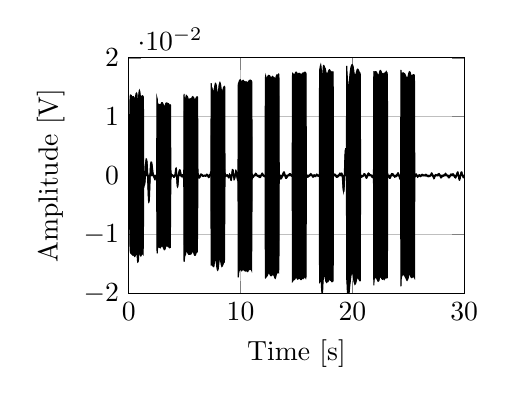
\begin{tikzpicture}

\begin{axis}[%
width=2.3in,
height=1.8in,
at={(0.758in,0.481in)},
xmin=0,
xmax=30,
xmajorgrids,
ymin=-0.02,
ymax=0.02,
ylabel={Amplitude [V]},
xlabel={Time [s]},
ymajorgrids,
axis background/.style={fill=white}
]
\addplot[fill=black,draw=black,forget plot] plot table[row sep=crcr]{%
2.08333333333333e-05	2.71797180175781e-05\\
0.0252733410493827	0.000192880630493164\\
0.0505258487654321	0.000219583511352539\\
0.0757783564814815	0.000324606895446777\\
0.101030864197531	0.0119782686233521\\
0.12628337191358	0.0132733583450317\\
0.15153587962963	0.0136597156524658\\
0.176788387345679	0.0136870145797729\\
0.202040895061728	0.0136398077011108\\
0.227293402777778	0.0136044025421143\\
0.252545910493827	0.0134916305541992\\
0.277798418209877	0.0134435892105103\\
0.303050925925926	0.0133676528930664\\
0.328303433641975	0.013298511505127\\
0.353555941358025	0.0132908821105957\\
0.378808449074074	0.0133390426635742\\
0.404060956790123	0.0133852958679199\\
0.429313464506173	0.0134091377258301\\
0.454565972222222	0.0132846832275391\\
0.479818479938272	0.0131728649139404\\
0.505070987654321	0.013127326965332\\
0.53032349537037	0.013005256652832\\
0.55557600308642	0.0130565166473389\\
0.580828510802469	0.0131419897079468\\
0.606081018518519	0.0132650136947632\\
0.631333526234568	0.0136377811431885\\
0.656586033950617	0.013906717300415\\
0.681838541666667	0.0139398574829102\\
0.707091049382716	0.014009952545166\\
0.732343557098765	0.0138951539993286\\
0.757596064814815	0.0131340026855469\\
0.782848572530864	0.0125246047973633\\
0.808101080246914	0.0120847225189209\\
0.833353587962963	0.0121047496795654\\
0.858606095679012	0.0126000642776489\\
0.883858603395062	0.0132580995559692\\
0.909111111111111	0.0139368772506714\\
0.934363618827161	0.0143285989761353\\
0.95961612654321	0.0144567489624023\\
0.984868634259259	0.0143048763275146\\
1.01012114197531	0.0140185356140137\\
1.03537364969136	0.0135726928710938\\
1.06062615740741	0.0131675004959106\\
1.08587866512346	0.0131186246871948\\
1.11113117283951	0.0132516622543335\\
1.13638368055556	0.0133669376373291\\
1.16163618827161	0.0134577751159668\\
1.18688869598765	0.013525128364563\\
1.2121412037037	0.0135258436203003\\
1.23739371141975	0.0135520696640015\\
1.2626462191358	0.0135167837142944\\
1.28789872685185	0.0133790969848633\\
1.3131512345679	0.0133394002914429\\
1.33840374228395	0.00212621688842773\\
1.36365625	0.000198721885681152\\
1.38890875771605	-0.000733494758605957\\
1.4141612654321	-0.00125908851623535\\
1.43941377314815	-0.00092923641204834\\
1.4646662808642	2.55107879638672e-05\\
1.48991878858025	0.00101137161254883\\
1.5151712962963	0.00201702117919922\\
1.54042380401235	0.00256431102752686\\
1.5656763117284	0.00282752513885498\\
1.59092881944444	0.00278055667877197\\
1.61618132716049	0.00261569023132324\\
1.64143383487654	0.00230515003204346\\
1.66668634259259	0.00142943859100342\\
1.69193885030864	0.000802040100097656\\
1.71719135802469	-0.000465273857116699\\
1.74244386574074	-0.00176858901977539\\
1.76769637345679	-0.00314795970916748\\
1.79294888117284	-0.00413775444030762\\
1.81820138888889	-0.00416898727416992\\
1.84345389660494	-0.00293600559234619\\
1.86870640432099	-0.00164687633514404\\
1.89395891203704	-0.000130534172058105\\
1.91921141975309	0.000895500183105469\\
1.94446392746914	0.00174665451049805\\
1.96971643518519	0.00211250782012939\\
1.99496894290123	0.00230598449707031\\
2.02022145061728	0.0022965669631958\\
2.04547395833333	0.00227689743041992\\
2.07072646604938	0.00209701061248779\\
2.09597897376543	0.00173783302307129\\
2.12123148148148	0.00134444236755371\\
2.14648398919753	0.000928759574890137\\
2.17173649691358	0.000492453575134277\\
2.19698900462963	0.000280857086181641\\
2.22224151234568	3.7074089050293e-05\\
2.24749402006173	-3.07559967041016e-05\\
2.27274652777778	-0.000232815742492676\\
2.29799903549383	-0.000373005867004395\\
2.32325154320988	-0.000491857528686523\\
2.34850405092593	-0.000524044036865234\\
2.37375655864198	-0.00048983097076416\\
2.39900906635802	-0.00031745433807373\\
2.42426157407407	-0.000228166580200195\\
2.44951408179012	-0.000116825103759766\\
2.47476658950617	-3.49283218383789e-05\\
2.50001909722222	-2.86102294921875e-06\\
2.52527160493827	0.0131807327270508\\
2.55052411265432	0.0129787921905518\\
2.57577662037037	0.0122307538986206\\
2.60102912808642	0.0119733810424805\\
2.62628163580247	0.0121581554412842\\
2.65153414351852	0.0121017694473267\\
2.67678665123457	0.0120164155960083\\
2.70203915895062	0.012006402015686\\
2.72729166666667	0.0119665861129761\\
2.75254417438272	0.0120497941970825\\
2.77779668209877	0.0120284557342529\\
2.80304918981481	0.0120289325714111\\
2.82830169753086	0.0119181871414185\\
2.85355420524691	0.0119922161102295\\
2.87880671296296	0.0121314525604248\\
2.90405922067901	0.0121816396713257\\
2.92931172839506	0.012296199798584\\
2.95456423611111	0.0123827457427979\\
2.97981674382716	0.0123804807662964\\
3.00506925154321	0.0123680830001831\\
3.03032175925926	0.0123096704483032\\
3.05557426697531	0.0122144222259521\\
3.08082677469136	0.0120468139648438\\
3.10607928240741	0.0120029449462891\\
3.13133179012346	0.0118519067764282\\
3.15658429783951	0.0116713047027588\\
3.18183680555556	0.0115656852722168\\
3.2070893132716	0.0115969181060791\\
3.23234182098765	0.0117167234420776\\
3.2575943287037	0.0118753910064697\\
3.28284683641975	0.0120331048965454\\
3.3080993441358	0.0122144222259521\\
3.33335185185185	0.0122911930084229\\
3.3586043595679	0.0123170614242554\\
3.38385686728395	0.0122699737548828\\
3.409109375	0.0123218297958374\\
3.43436188271605	0.01230788230896\\
3.4596143904321	0.0122936964035034\\
3.48486689814815	0.0122591257095337\\
3.5101194058642	0.0121793746948242\\
3.53537191358025	0.0122112035751343\\
3.5606244212963	0.012218713760376\\
3.58587692901235	0.0120950937271118\\
3.61112943672839	0.0120012760162354\\
3.63638194444444	0.0119942426681519\\
3.66163445216049	0.0119779109954834\\
3.68688695987654	0.0119713544845581\\
3.71213946759259	0.0120042562484741\\
3.73739197530864	0.0119483470916748\\
3.76264448302469	0.00140035152435303\\
3.78789699074074	0.000461459159851074\\
3.81314949845679	0.000228643417358398\\
3.83840200617284	0.000122308731079102\\
3.86365451388889	0.00018775463104248\\
3.88890702160494	0.000143051147460938\\
3.91415952932099	9.60826873779297e-05\\
3.93941203703704	3.83853912353516e-05\\
3.96466454475309	3.01599502563477e-05\\
3.98991705246914	-4.05311584472656e-06\\
4.01516956018518	-7.51018524169922e-05\\
4.04042206790123	-0.000198602676391602\\
4.06567457561728	-0.000174880027770996\\
4.09092708333333	-0.000170588493347168\\
4.11617959104938	-7.84397125244141e-05\\
4.14143209876543	0.000242471694946289\\
4.16668460648148	0.00061953067779541\\
4.19193711419753	0.00105559825897217\\
4.21718962191358	0.00124335289001465\\
4.24244212962963	0.00129139423370361\\
4.26769463734568	0.00111246109008789\\
4.29294714506173	0.000468969345092773\\
4.31819965277778	-0.000456333160400391\\
4.34345216049383	-0.00124490261077881\\
4.36870466820988	-0.00180208683013916\\
4.39395717592593	-0.00133395195007324\\
4.41920968364198	-0.000530719757080078\\
4.44446219135802	-4.05311584472656e-05\\
4.46971469907407	0.000434398651123047\\
4.49496720679012	0.000670433044433594\\
4.52021971450617	0.000893712043762207\\
4.54547222222222	0.000962257385253906\\
4.57072472993827	0.000990629196166992\\
4.59597723765432	0.000925421714782715\\
4.62122974537037	0.000837922096252441\\
4.64648225308642	0.00060117244720459\\
4.67173476080247	0.00031888484954834\\
4.69698726851852	1.08480453491211e-05\\
4.72223977623457	-6.46114349365234e-05\\
4.74749228395062	4.62532043457031e-05\\
4.77274479166667	7.72476196289063e-05\\
4.79799729938272	0.000130534172058105\\
4.82324980709877	0.000133872032165527\\
4.84850231481482	2.68220901489258e-05\\
4.87375482253086	-0.000166893005371094\\
4.89900733024691	-0.00031590461730957\\
4.92425983796296	-0.000426411628723145\\
4.94951234567901	0.0138906240463257\\
4.97476485339506	0.0127924680709839\\
5.00001736111111	0.0127823352813721\\
5.02526986882716	0.0127456188201904\\
5.05052237654321	0.012772798538208\\
5.07577488425926	0.0129667520523071\\
5.10102739197531	0.0132062435150146\\
5.12627989969136	0.0134183168411255\\
5.15153240740741	0.0136046409606934\\
5.17678491512346	0.0135563611984253\\
5.20203742283951	0.0135209560394287\\
5.22728993055556	0.0134320259094238\\
5.2525424382716	0.0134093761444092\\
5.27779494598765	0.0132806301116943\\
5.3030474537037	0.0131157636642456\\
5.32829996141975	0.0129809379577637\\
5.3535524691358	0.0129413604736328\\
5.37880497685185	0.0128811597824097\\
5.4040574845679	0.0128850936889648\\
5.42930999228395	0.012834906578064\\
5.4545625	0.0129283666610718\\
5.47981500771605	0.0130480527877808\\
5.5050675154321	0.0130259990692139\\
5.53032002314815	0.0129679441452026\\
5.5555725308642	0.0129989385604858\\
5.58082503858025	0.0130027532577515\\
5.6060775462963	0.0131098031997681\\
5.63133005401235	0.0131270885467529\\
5.65658256172839	0.0132246017456055\\
5.68183506944444	0.0133410692214966\\
5.70708757716049	0.0133851766586304\\
5.73234008487654	0.0134118795394897\\
5.75759259259259	0.0132910013198853\\
5.78284510030864	0.0132763385772705\\
5.80809760802469	0.0132464170455933\\
5.83335011574074	0.0131045579910278\\
5.85860262345679	0.0130085945129395\\
5.88385513117284	0.012847900390625\\
5.90910763888889	0.0127744674682617\\
5.93436014660494	0.0128093957901001\\
5.95961265432099	0.0128616094589233\\
5.98486516203704	0.0129320621490479\\
6.01011766975309	0.0131421089172363\\
6.03537017746914	0.0131816864013672\\
6.06062268518518	0.0133038759231567\\
6.08587519290123	0.0133326053619385\\
6.11112770061728	0.0133798122406006\\
6.13638020833333	0.0133734941482544\\
6.16163271604938	0.0133055448532104\\
6.18688522376543	0.00129294395446777\\
6.21213773148148	0.000391721725463867\\
6.23739023919753	0.000118851661682129\\
6.26264274691358	-6.7591667175293e-05\\
6.28789525462963	-0.00014650821685791\\
6.31314776234568	-0.000262737274169922\\
6.33840027006173	-0.000207424163818359\\
6.36365277777778	-0.000160098075866699\\
6.38890528549383	-3.62396240234375e-05\\
6.41415779320988	0.000113129615783691\\
6.43941030092593	0.000204920768737793\\
6.46466280864198	0.000273823738098145\\
6.48991531635802	0.000244855880737305\\
6.51516782407407	0.000198602676391602\\
6.54042033179012	0.000207901000976563\\
6.56567283950617	0.000176548957824707\\
6.59092534722222	9.56058502197266e-05\\
6.61617785493827	1.53779983520508e-05\\
6.64143036265432	-4.20808792114258e-05\\
6.66668287037037	-2.02655792236328e-06\\
6.69193537808642	-1.70469284057617e-05\\
6.71718788580247	3.08752059936523e-05\\
6.74244039351852	4.80413436889648e-05\\
6.76769290123457	5.51939010620117e-05\\
6.79294540895062	6.13927841186523e-05\\
6.81819791666667	1.4185905456543e-05\\
6.84345042438272	2.51531600952148e-05\\
6.86870293209877	-3.33786010742188e-06\\
6.89395543981481	-1.58548355102539e-05\\
6.91920794753086	0.000109314918518066\\
6.94446045524691	0.00016486644744873\\
6.96971296296296	0.000245809555053711\\
6.99496547067901	0.000245332717895508\\
7.02021797839506	0.000184535980224609\\
7.04547048611111	0.000141501426696777\\
7.07072299382716	0.000122666358947754\\
7.09597550154321	-4.24385070800781e-05\\
7.12122800925926	-0.000117182731628418\\
7.14648051697531	-0.000206112861633301\\
7.17173302469136	-0.000195622444152832\\
7.19698553240741	-4.50611114501953e-05\\
7.22223804012346	2.41994857788086e-05\\
7.24749054783951	0.000180721282958984\\
7.27274305555556	0.000224471092224121\\
7.2979955632716	0.000301599502563477\\
7.32324807098765	0.000630378723144531\\
7.3485005787037	0.000650882720947266\\
7.37375308641975	0.0156896114349365\\
7.3990055941358	0.0150365829467773\\
7.42425810185185	0.0149332284927368\\
7.4495106095679	0.0148735046386719\\
7.47476311728395	0.0145994424819946\\
7.500015625	0.0142728090286255\\
7.52526813271605	0.0143123865127563\\
7.5505206404321	0.0141353607177734\\
7.57577314814815	0.0140994787216187\\
7.6010256558642	0.0140562057495117\\
7.62627816358025	0.0144972801208496\\
7.6515306712963	0.0147725343704224\\
7.67678317901235	0.0148419141769409\\
7.70203568672839	0.0152887105941772\\
7.72728819444444	0.015468955039978\\
7.75254070216049	0.0156747102737427\\
7.77779320987654	0.0156437158584595\\
7.80304571759259	0.0155001878738403\\
7.82829822530864	0.0153249502182007\\
7.85355073302469	0.0149215459823608\\
7.87880324074074	0.0144649744033813\\
7.90405574845679	0.0139764547348022\\
7.92930825617284	0.0136035680770874\\
7.95456076388889	0.0135245323181152\\
7.97981327160494	0.0136982202529907\\
8.00506577932099	0.0140670537948608\\
8.03031828703704	0.0143532752990723\\
8.05557079475309	0.0147926807403564\\
8.08082330246914	0.0153083801269531\\
8.10607581018519	0.015499472618103\\
8.13132831790123	0.0156772136688232\\
8.15658082561728	0.0157968997955322\\
8.18183333333333	0.0156925916671753\\
8.20708584104938	0.0154823064804077\\
8.23233834876543	0.0152593851089478\\
8.25759085648148	0.014828085899353\\
8.28284336419753	0.0144996643066406\\
8.30809587191358	0.0143203735351563\\
8.33334837962963	0.0142027139663696\\
8.35860088734568	0.0142422914505005\\
8.38385339506173	0.0143022537231445\\
8.40910590277778	0.01442551612854\\
8.43435841049383	0.0146499872207642\\
8.45961091820988	0.0148167610168457\\
8.48486342592593	0.0149878263473511\\
8.51011593364198	0.0150655508041382\\
8.53536844135802	0.0150963068008423\\
8.56062094907407	0.0151380300521851\\
8.58587345679012	0.0150313377380371\\
8.61112596450617	0.000926375389099121\\
8.63637847222222	0.000237107276916504\\
8.66163097993827	1.70469284057617e-05\\
8.68688348765432	-1.04904174804688e-05\\
8.71213599537037	7.79628753662109e-05\\
8.73738850308642	8.10623168945313e-05\\
8.76264101080247	9.01222229003906e-05\\
8.78789351851852	0.000140666961669922\\
8.81314602623457	0.000134706497192383\\
8.83839853395062	6.63995742797852e-05\\
8.86365104166667	1.8000602722168e-05\\
8.88890354938272	-0.000120162963867188\\
8.91415605709877	-0.00020444393157959\\
8.93940856481481	-0.000177621841430664\\
8.96466107253086	-6.72340393066406e-05\\
8.98991358024691	7.18832015991211e-05\\
9.01516608796296	0.000251293182373047\\
9.04041859567901	0.000190377235412598\\
9.06567110339506	0.000151991844177246\\
9.09092361111111	-7.84397125244141e-05\\
9.11617611882716	-0.000372886657714844\\
9.14142862654321	-0.000590682029724121\\
9.16668113425926	-0.00061953067779541\\
9.19193364197531	-0.000303745269775391\\
9.21718614969136	0.00022578239440918\\
9.24243865740741	0.000708937644958496\\
9.26769116512346	0.00102901458740234\\
9.29294367283951	0.00101268291473389\\
9.31819618055556	0.000956416130065918\\
9.34344868827161	0.000914931297302246\\
9.36870119598765	0.000367522239685059\\
9.3939537037037	2.45571136474609e-05\\
9.41920621141975	-0.000287413597106934\\
9.4444587191358	-0.000396251678466797\\
9.46971122685185	-0.000282764434814453\\
9.4949637345679	-5.55515289306641e-05\\
9.52021624228395	0.000377655029296875\\
9.54546875	0.000602841377258301\\
9.57072125771605	0.000919580459594727\\
9.5959737654321	0.000896334648132324\\
9.62122627314815	0.000671863555908203\\
9.6464787808642	0.000562429428100586\\
9.67173128858025	0.000257372856140137\\
9.6969837962963	-0.000269532203674316\\
9.72223630401235	-0.000421762466430664\\
9.7474888117284	-0.000730991363525391\\
9.77274131944444	-0.000650405883789063\\
9.79799382716049	0.0154277086257935\\
9.82324633487654	0.0156807899475098\\
9.84849884259259	0.0157598257064819\\
9.87375135030864	0.0159609317779541\\
9.89900385802469	0.0161114931106567\\
9.92425636574074	0.0161769390106201\\
9.94950887345679	0.0162290334701538\\
9.97476138117284	0.0162595510482788\\
10.0000138888889	0.0160911083221436\\
10.0252663966049	0.0160559415817261\\
10.050518904321	0.0159459114074707\\
10.075771412037	0.0158594846725464\\
10.1010239197531	0.0158390998840332\\
10.1262764274691	0.0159010887145996\\
10.1515289351852	0.0160681009292603\\
10.1767814429012	0.0160746574401855\\
10.2020339506173	0.0161263942718506\\
10.2272864583333	0.0161761045455933\\
10.2525389660494	0.0161302089691162\\
10.2777914737654	0.0160362720489502\\
10.3030439814815	0.0160095691680908\\
10.3282964891975	0.0159236192703247\\
10.3535489969136	0.0159534215927124\\
10.3788015046296	0.0158895254135132\\
10.4040540123457	0.0158728361129761\\
10.4293065200617	0.0158777236938477\\
10.4545590277778	0.0158460140228271\\
10.4798115354938	0.015931248664856\\
10.5050640432099	0.0159186124801636\\
10.5303165509259	0.0159024000167847\\
10.555569058642	0.0158482789993286\\
10.580821566358	0.015781044960022\\
10.6060740740741	0.0157147645950317\\
10.6313265817901	0.0157208442687988\\
10.6565790895062	0.0157356262207031\\
10.6818315972222	0.0159025192260742\\
10.7070841049383	0.0159567594528198\\
10.7323366126543	0.0160346031188965\\
10.7575891203704	0.0160861015319824\\
10.7828416280864	0.0160651206970215\\
10.8080941358025	0.0160901546478271\\
10.8333466435185	0.016063928604126\\
10.8585991512346	0.0161927938461304\\
10.8838516589506	0.0161173343658447\\
10.9091041666667	0.0161306858062744\\
10.9343566743827	0.0161368846893311\\
10.9596091820988	0.0161256790161133\\
10.9848616898148	0.0159846544265747\\
11.0101141975309	0.0159024000167847\\
11.0353667052469	0.000484466552734375\\
11.060619212963	-4.20808792114258e-05\\
11.085871720679	-0.000198245048522949\\
11.1111242283951	-0.000219464302062988\\
11.1363767361111	-0.000158071517944336\\
11.1616292438272	-0.000123023986816406\\
11.1868817515432	-8.08238983154297e-05\\
11.2121342592593	6.79492950439453e-05\\
11.2373867669753	0.000106930732727051\\
11.2626392746914	0.000181078910827637\\
11.2878917824074	0.000208735466003418\\
11.3131442901235	0.000313282012939453\\
11.3383967978395	0.000393390655517578\\
11.3636493055556	0.000383138656616211\\
11.3889018132716	0.000328779220581055\\
11.4141543209877	0.000310063362121582\\
11.4394068287037	0.000229954719543457\\
11.4646593364198	0.000151157379150391\\
11.4899118441358	5.84125518798828e-05\\
11.5151643518519	3.34978103637695e-05\\
11.5404168595679	-4.55379486083984e-05\\
11.565669367284	-5.91278076171875e-05\\
11.590921875	-7.34329223632813e-05\\
11.6161743827161	-0.000102996826171875\\
11.6414268904321	-0.000104308128356934\\
11.6666793981481	-0.000190258026123047\\
11.6919319058642	-0.000185608863830566\\
11.7171844135802	-0.000193119049072266\\
11.7424369212963	-0.000184893608093262\\
11.7676894290123	-0.000196099281311035\\
11.7929419367284	-0.000140070915222168\\
11.8181944444444	1.53779983520508e-05\\
11.8434469521605	0.000145673751831055\\
11.8686994598765	0.000226259231567383\\
11.8939519675926	0.000336289405822754\\
11.9192044753086	0.000395894050598145\\
11.9444569830247	0.000421047210693359\\
11.9697094907407	0.000374794006347656\\
11.9949619984568	0.000291228294372559\\
12.0202145061728	0.000190615653991699\\
12.0454670138889	0.000115513801574707\\
12.0707195216049	3.0517578125e-05\\
12.095972029321	-2.41994857788086e-05\\
12.121224537037	-8.46385955810547e-05\\
12.1464770447531	-7.55786895751953e-05\\
12.1717295524691	-9.41753387451172e-05\\
12.1969820601852	-5.48362731933594e-06\\
12.2222345679012	0.0165671110153198\\
12.2474870756173	0.0168999433517456\\
12.2727395833333	0.0166717767715454\\
12.2979920910494	0.0165742635726929\\
12.3232445987654	0.0165170431137085\\
12.3484971064815	0.0165308713912964\\
12.3737496141975	0.016585111618042\\
12.3990021219136	0.0166263580322266\\
12.4242546296296	0.0167803764343262\\
12.4495071373457	0.0168399810791016\\
12.4747596450617	0.0169746875762939\\
12.5000121527778	0.0169860124588013\\
12.5252646604938	0.0170214176177979\\
12.5505171682099	0.0169990062713623\\
12.5757696759259	0.0169893503189087\\
12.601022183642	0.0169556140899658\\
12.626274691358	0.0168999433517456\\
12.6515271990741	0.0167281627655029\\
12.6767797067901	0.0166318416595459\\
12.7020322145062	0.0165399312973022\\
12.7272847222222	0.0165116786956787\\
12.7525372299383	0.0165554285049438\\
12.7777897376543	0.01661217212677\\
12.8030422453704	0.0167293548583984\\
12.8282947530864	0.0167727470397949\\
12.8535472608025	0.0168174505233765\\
12.8787997685185	0.0166926383972168\\
12.9040522762346	0.0167468786239624\\
12.9293047839506	0.0166680812835693\\
12.9545572916667	0.016689658164978\\
12.9798097993827	0.0166734457015991\\
13.0050623070988	0.0166347026824951\\
13.0303148148148	0.016505241394043\\
13.0555673225309	0.0163514614105225\\
13.0808198302469	0.0162187814712524\\
13.106072337963	0.0161361694335938\\
13.131324845679	0.0162808895111084\\
13.1565773533951	0.0165536403656006\\
13.1818298611111	0.0167999267578125\\
13.2070823688272	0.0169224739074707\\
13.2323348765432	0.017076849937439\\
13.2575873842593	0.017071008682251\\
13.2828398919753	0.0170369148254395\\
13.3080923996914	0.0170255899429321\\
13.3333449074074	0.0170601606369019\\
13.3585974151235	0.0171662569046021\\
13.3838499228395	0.0171995162963867\\
13.4091024305556	0.017237663269043\\
13.4343549382716	0.0171002149581909\\
13.4596074459877	0.00082862377166748\\
13.4848599537037	0.000102758407592773\\
13.5101124614198	-9.918212890625e-05\\
13.5353649691358	-0.000249147415161133\\
13.5606174768519	-0.000396728515625\\
13.5858699845679	-0.000394225120544434\\
13.611122492284	-0.00046849250793457\\
13.636375	-0.000432133674621582\\
13.6616275077161	-0.000347495079040527\\
13.6868800154321	-0.000221014022827148\\
13.7121325231481	-9.14335250854492e-05\\
13.7373850308642	-1.00135803222656e-05\\
13.7626375385802	0.000199437141418457\\
13.7878900462963	0.00036931037902832\\
13.8131425540123	0.000469803810119629\\
13.8383950617284	0.000552892684936523\\
13.8636475694444	0.000609636306762695\\
13.8889000771605	0.000621199607849121\\
13.9141525848765	0.000609278678894043\\
13.9394050925926	0.000482797622680664\\
13.9646576003086	0.000282883644104004\\
13.9899101080247	7.42673873901367e-05\\
14.0151626157407	-0.000166416168212891\\
14.0404151234568	-0.000336170196533203\\
14.0656676311728	-0.000344991683959961\\
14.0909201388889	-0.000310778617858887\\
14.1161726466049	-0.000333666801452637\\
14.141425154321	-0.000180602073669434\\
14.166677662037	-0.00015723705291748\\
14.1919301697531	-6.13927841186523e-05\\
14.2171826774691	-1.87158584594727e-05\\
14.2424351851852	4.25577163696289e-05\\
14.2676876929012	0.000150203704833984\\
14.2929402006173	0.000175714492797852\\
14.3181927083333	0.000205278396606445\\
14.3434452160494	0.000236988067626953\\
14.3686977237654	0.000314712524414063\\
14.3939502314815	0.000324130058288574\\
14.4192027391975	0.000327944755554199\\
14.4444552469136	0.000308752059936523\\
14.4697077546296	0.00026547908782959\\
14.4949602623457	0.000200629234313965\\
14.5202127700617	0.000146389007568359\\
14.5454652777778	6.92605972290039e-05\\
14.5707177854938	7.15255737304688e-06\\
14.5959702932099	3.00407409667969e-05\\
14.6212228009259	1.62124633789063e-05\\
14.646475308642	0.0169292688369751\\
14.671727816358	0.0173319578170776\\
14.6969803240741	0.0172630548477173\\
14.7222328317901	0.0172011852264404\\
14.7474853395062	0.0171821117401123\\
14.7727378472222	0.0171287059783936\\
14.7979903549383	0.0171319246292114\\
14.8232428626543	0.0171495676040649\\
14.8484953703704	0.0171682834625244\\
14.8737478780864	0.0171934366226196\\
14.8990003858025	0.0174195766448975\\
14.9242528935185	0.0175316333770752\\
14.9495054012346	0.0175597667694092\\
14.9747579089506	0.0175731182098389\\
15.0000104166667	0.0175539255142212\\
15.0252629243827	0.0175000429153442\\
15.0505154320988	0.0173577070236206\\
15.0757679398148	0.0172542333602905\\
15.1010204475309	0.0171407461166382\\
15.1262729552469	0.0171658992767334\\
15.151525462963	0.0172443389892578\\
15.176777970679	0.0172475576400757\\
15.2020304783951	0.0173439979553223\\
15.2272829861111	0.0173681974411011\\
15.2525354938272	0.0173213481903076\\
15.2777880015432	0.0173455476760864\\
15.3030405092593	0.0173231363296509\\
15.3282930169753	0.0172563791275024\\
15.3535455246914	0.017225980758667\\
15.3787980324074	0.0171550512313843\\
15.4040505401235	0.0170636177062988\\
15.4293030478395	0.0170685052871704\\
15.4545555555556	0.0171319246292114\\
15.4798080632716	0.0172151327133179\\
15.5050605709877	0.0172789096832275\\
15.5303130787037	0.0173686742782593\\
15.5555655864198	0.0173188447952271\\
15.5808180941358	0.0173131227493286\\
15.6060706018519	0.0173306465148926\\
15.6313231095679	0.017390251159668\\
15.656575617284	0.0174404382705688\\
15.681828125	0.0174127817153931\\
15.7070806327161	0.0175391435623169\\
15.7323331404321	0.0175487995147705\\
15.7575856481481	0.0175501108169556\\
15.7828381558642	0.0175542831420898\\
15.8080906635802	0.0174723863601685\\
15.8333431712963	0.0174212455749512\\
15.8585956790123	0.0172785520553589\\
15.8838481867284	0.000405669212341309\\
15.9091006944444	8.47578048706055e-05\\
15.9343532021605	-6.92605972290039e-05\\
15.9596057098765	-2.07424163818359e-05\\
15.9848582175926	-0.000122547149658203\\
16.0101107253086	-0.00012052059173584\\
16.0353632330247	-0.000148892402648926\\
16.0606157407407	-0.000107645988464355\\
16.0858682484568	-3.40938568115234e-05\\
16.1111207561728	-4.16040420532227e-05\\
16.1363732638889	8.47578048706055e-05\\
16.1616257716049	0.000107288360595703\\
16.186878279321	0.000143051147460938\\
16.212130787037	0.000160574913024902\\
16.2373832947531	0.000275850296020508\\
16.2626358024691	0.000192046165466309\\
16.2878883101852	0.000250697135925293\\
16.3131408179012	0.000265836715698242\\
16.3383933256173	0.000269889831542969\\
16.3636458333333	0.000122189521789551\\
16.3888983410494	0.00011444091796875\\
16.4141508487654	4.45842742919922e-05\\
16.4394033564815	-3.42130661010742e-05\\
16.4646558641975	-0.000105977058410645\\
16.4899083719136	-1.00135803222656e-05\\
16.5151608796296	-0.0001068115234375\\
16.5404133873457	6.79492950439453e-06\\
16.5656658950617	8.84532928466797e-05\\
16.5909184027778	6.46114349365234e-05\\
16.6161709104938	0.000111937522888184\\
16.6414234182099	6.18696212768555e-05\\
16.6666759259259	7.46250152587891e-05\\
16.691928433642	-3.75509262084961e-05\\
16.717180941358	2.86102294921875e-06\\
16.7424334490741	6.50882720947266e-05\\
16.7676859567901	0.000104427337646484\\
16.7929384645062	0.000123023986816406\\
16.8181909722222	0.000252127647399902\\
16.8434434799383	0.000231504440307617\\
16.8686959876543	0.000136375427246094\\
16.8939484953704	7.71284103393555e-05\\
16.9192010030864	8.46385955810547e-05\\
16.9444535108025	9.02414321899414e-05\\
16.9697060185185	8.14199447631836e-05\\
16.9949585262346	0.000124812126159668\\
17.0202110339506	0.000126481056213379\\
17.0454635416667	5.80549240112305e-05\\
17.0707160493827	0.0179164409637451\\
17.0959685570988	0.0180661678314209\\
17.1212210648148	0.0184476375579834\\
17.1464735725309	0.0186307430267334\\
17.1717260802469	0.0187876224517822\\
17.196978587963	0.0185372829437256\\
17.222231095679	0.0179513692855835\\
17.2474836033951	0.0168821811676025\\
17.2727361111111	0.0159904956817627\\
17.2979886188272	0.0154684782028198\\
17.3232411265432	0.0159759521484375\\
17.3484936342593	0.0165970325469971\\
17.3737461419753	0.0177416801452637\\
17.3989986496914	0.0184311866760254\\
17.4242511574074	0.0186929702758789\\
17.4495036651235	0.0186983346939087\\
17.4747561728395	0.0186036825180054\\
17.5000086805556	0.0184463262557983\\
17.5252611882716	0.0182918310165405\\
17.5505136959877	0.0182555913925171\\
17.5757662037037	0.0181587934494019\\
17.6010187114198	0.0178960561752319\\
17.6262712191358	0.0177195072174072\\
17.6515237268519	0.0174219608306885\\
17.6767762345679	0.0173271894454956\\
17.702028742284	0.0173096656799316\\
17.72728125	0.0173647403717041\\
17.7525337577161	0.0173664093017578\\
17.7777862654321	0.0174031257629395\\
17.8030387731481	0.0174136161804199\\
17.8282912808642	0.0174782276153564\\
17.8535437885803	0.0175955295562744\\
17.8787962962963	0.0177769660949707\\
17.9040488040123	0.0178405046463013\\
17.9293013117284	0.0179694890975952\\
17.9545538194444	0.0179864168167114\\
17.9798063271605	0.0179113149642944\\
18.0050588348765	0.0178525447845459\\
18.0303113425926	0.0176674127578735\\
18.0555638503086	0.0176661014556885\\
18.0808163580247	0.0176839828491211\\
18.1060688657407	0.0176535844802856\\
18.1313213734568	0.0175237655639648\\
18.1565738811728	0.017460823059082\\
18.1818263888889	0.0174012184143066\\
18.2070788966049	0.0174828767776489\\
18.232331404321	0.0174508094787598\\
18.257583912037	0.017616868019104\\
18.2828364197531	0.0175806283950806\\
18.3080889274691	0.000448226928710938\\
18.3333414351852	0.00021660327911377\\
18.3585939429012	0.00025629997253418\\
18.3838464506173	0.000190377235412598\\
18.4090989583333	0.000196099281311035\\
18.4343514660494	0.000238776206970215\\
18.4596039737654	0.000233769416809082\\
18.4848564814815	0.000162005424499512\\
18.5101089891975	0.000110983848571777\\
18.5353614969136	-2.21729278564453e-05\\
18.5606140046296	-2.96831130981445e-05\\
18.5858665123457	-9.93013381958008e-05\\
18.6111190200617	-0.000138998031616211\\
18.6363715277778	-0.000132203102111816\\
18.6616240354938	-0.000133991241455078\\
18.6868765432099	-0.000164389610290527\\
18.7121290509259	-8.96453857421875e-05\\
18.737381558642	-5.50746917724609e-05\\
18.762634066358	7.43865966796875e-05\\
18.7878865740741	0.000127196311950684\\
18.8131390817901	0.000230312347412109\\
18.8383915895062	0.000272393226623535\\
18.8636440972222	0.000393390655517578\\
18.8888966049383	0.000400662422180176\\
18.9141491126543	0.000297904014587402\\
18.9394016203704	0.000269889831542969\\
18.9646541280864	0.000294923782348633\\
18.9899066358025	0.000373482704162598\\
19.0151591435185	0.000348806381225586\\
19.0404116512346	0.000412225723266602\\
19.0656641589506	0.000396013259887695\\
19.0909166666667	0.000279664993286133\\
19.1161691743827	-5.59091567993164e-05\\
19.1414216820988	-0.000618696212768555\\
19.1666741898148	-0.00137102603912354\\
19.1919266975309	-0.00211083889007568\\
19.2171792052469	-0.00251805782318115\\
19.242431712963	-0.00203609466552734\\
19.267684220679	-0.000851988792419434\\
19.2929367283951	0.000642061233520508\\
19.3181892361111	0.00228226184844971\\
19.3434417438272	0.00357353687286377\\
19.3686942515432	0.00432217121124268\\
19.3939467592593	0.00450289249420166\\
19.4191992669753	0.00446105003356934\\
19.4444517746914	0.00392818450927734\\
19.4697042824074	0.00306880474090576\\
19.4949567901235	0.0186182260513306\\
19.5202092978395	0.0174990892410278\\
19.5454618055556	0.0167573690414429\\
19.5707143132716	0.0156563520431519\\
19.5959668209877	0.0149348974227905\\
19.6212193287037	0.01460862159729\\
19.6464718364198	0.014657735824585\\
19.6717243441358	0.0149654150009155\\
19.6969768518519	0.0154080390930176\\
19.7222293595679	0.0158551931381226\\
19.747481867284	0.0163990259170532\\
19.772734375	0.0168666839599609\\
19.797986882716	0.0174103975296021\\
19.8232393904321	0.0177158117294312\\
19.8484918981482	0.0181130170822144\\
19.8737444058642	0.0183916091918945\\
19.8989969135802	0.0185835361480713\\
19.9242494212963	0.0186495780944824\\
19.9495019290123	0.0187809467315674\\
19.9747544367284	0.0187575817108154\\
20.0000069444444	0.0188125371932983\\
20.0252594521605	0.0186846256256104\\
20.0505119598765	0.0186182260513306\\
20.0757644675926	0.0184367895126343\\
20.1010169753086	0.0180631875991821\\
20.1262694830247	0.017815113067627\\
20.1515219907407	0.01743483543396\\
20.1767744984568	0.017147421836853\\
20.2020270061728	0.0169249773025513\\
20.2272795138889	0.0168775320053101\\
20.2525320216049	0.0168746709823608\\
20.277784529321	0.0169830322265625\\
20.303037037037	0.0171991586685181\\
20.3282895447531	0.0172855854034424\\
20.3535420524691	0.0174849033355713\\
20.3787945601852	0.0177160501480103\\
20.4040470679012	0.0177884101867676\\
20.4292995756173	0.0180319547653198\\
20.4545520833333	0.0180799961090088\\
20.4798045910494	0.018064022064209\\
20.5050570987654	0.0180245637893677\\
20.5303096064815	0.0179439783096313\\
20.5555621141975	0.0178685188293457\\
20.5808146219136	0.0177570581436157\\
20.6060671296296	0.0175374746322632\\
20.6313196373457	0.0175430774688721\\
20.6565721450617	0.017493724822998\\
20.6818246527778	0.0174106359481812\\
20.7070771604938	0.0171592235565186\\
20.7323296682099	0.000139713287353516\\
20.7575821759259	-3.37362289428711e-05\\
20.782834683642	-0.000109195709228516\\
20.808087191358	-9.17911529541016e-05\\
20.8333396990741	-7.46250152587891e-05\\
20.8585922067901	-4.33921813964844e-05\\
20.8838447145062	-7.25984573364258e-05\\
20.9090972222222	-8.38041305541992e-05\\
20.9343497299383	-2.80141830444336e-05\\
20.9596022376543	3.58819961547852e-05\\
20.9848547453704	4.8518180847168e-05\\
21.0101072530864	0.000126957893371582\\
21.0353597608025	0.000322937965393066\\
21.0606122685185	0.000291347503662109\\
21.0858647762346	0.00032806396484375\\
21.1111172839506	0.000323891639709473\\
21.1363697916667	0.000241279602050781\\
21.1616222993827	0.00010228157043457\\
21.1868748070988	-1.13248825073242e-05\\
21.2121273148148	-0.000200152397155762\\
21.2373798225309	-0.000227689743041992\\
21.2626323302469	-0.000326991081237793\\
21.287884837963	-0.00032341480255127\\
21.313137345679	-0.000106692314147949\\
21.3383898533951	1.76429748535156e-05\\
21.3636423611111	0.00022125244140625\\
21.3888948688272	0.000350832939147949\\
21.4141473765432	0.000402212142944336\\
21.4393998842593	0.000428199768066406\\
21.4646523919753	0.000411510467529297\\
21.4899048996914	0.000369668006896973\\
21.5151574074074	0.000343918800354004\\
21.5404099151235	0.000272989273071289\\
21.5656624228395	0.000220298767089844\\
21.5909149305556	0.000177383422851563\\
21.6161674382716	0.000154852867126465\\
21.6414199459877	0.000129818916320801\\
21.6666724537037	0.000105977058410645\\
21.6919249614198	0.000100135803222656\\
21.7171774691358	-1.95503234863281e-05\\
21.7424299768519	-5.340576171875e-05\\
21.7676824845679	-0.000153064727783203\\
21.792934992284	-0.000183582305908203\\
21.8181875	-0.000210165977478027\\
21.8434400077161	-0.000201106071472168\\
21.8686925154321	-0.000120639801025391\\
21.8939450231481	-4.49419021606445e-05\\
21.9191975308642	0.0177475214004517\\
21.9444500385803	0.0173670053482056\\
21.9697025462963	0.0173903703689575\\
21.9949550540123	0.0174099206924438\\
22.0202075617284	0.0175341367721558\\
22.0454600694444	0.0176265239715576\\
22.0707125771605	0.0176255702972412\\
22.0959650848765	0.0176335573196411\\
22.1212175925926	0.0175776481628418\\
22.1464701003086	0.0175797939300537\\
22.1717226080247	0.0175366401672363\\
22.1969751157407	0.0173623561859131\\
22.2222276234568	0.017267107963562\\
22.2474801311728	0.0171732902526855\\
22.2727326388889	0.0169675350189209\\
22.2979851466049	0.0169329643249512\\
22.323237654321	0.0168830156326294\\
22.348490162037	0.0169788599014282\\
22.3737426697531	0.0170691013336182\\
22.3989951774691	0.0172792673110962\\
22.4242476851852	0.0174456834793091\\
22.4495001929012	0.0176714658737183\\
22.4747527006173	0.0178101062774658\\
22.5000052083333	0.0178617238998413\\
22.5252577160494	0.0178629159927368\\
22.5505102237654	0.0177403688430786\\
22.5757627314815	0.017638087272644\\
22.6010152391975	0.017555832862854\\
22.6262677469136	0.0173798799514771\\
22.6515202546296	0.0172560214996338\\
22.6767727623457	0.01722252368927\\
22.7020252700617	0.0172896385192871\\
22.7272777777778	0.0172810554504395\\
22.7525302854938	0.0172203779220581\\
22.7777827932099	0.0172380208969116\\
22.8030353009259	0.0172601938247681\\
22.828287808642	0.0173335075378418\\
22.853540316358	0.0172879695892334\\
22.8787928240741	0.0173248052597046\\
22.9040453317901	0.0173823833465576\\
22.9292978395062	0.0174615383148193\\
22.9545503472222	0.0174990892410278\\
22.9798028549383	0.0174890756607056\\
23.0050553626543	0.0175430774688721\\
23.0303078703704	0.0176382064819336\\
23.0555603780864	0.0175291299819946\\
23.0808128858025	0.0175257921218872\\
23.1060653935185	0.0174691677093506\\
23.1313179012346	0.0169287919998169\\
23.1565704089506	0.000443935394287109\\
23.1818229166667	0.00018155574798584\\
23.2070754243827	-8.70227813720703e-06\\
23.2323279320988	-7.49826431274414e-05\\
23.2575804398148	-9.97781753540039e-05\\
23.2828329475309	-0.000157356262207031\\
23.3080854552469	-0.000261664390563965\\
23.333337962963	-0.000339508056640625\\
23.358590470679	-0.000370383262634277\\
23.3838429783951	-0.000281095504760742\\
23.4090954861111	-0.000164031982421875\\
23.4343479938272	-6.07967376708984e-05\\
23.4596005015432	0.000153064727783203\\
23.4848530092593	0.000249981880187988\\
23.5101055169753	0.000330924987792969\\
23.5353580246914	0.00034642219543457\\
23.5606105324074	0.000332117080688477\\
23.5858630401235	0.000333070755004883\\
23.6111155478395	0.000329732894897461\\
23.6363680555556	0.000268697738647461\\
23.6616205632716	0.000220298767089844\\
23.6868730709877	0.000146865844726563\\
23.7121255787037	3.57627868652344e-07\\
23.7373780864198	-1.20401382446289e-05\\
23.7626305941358	-7.67707824707031e-05\\
23.7878831018519	-0.000118017196655273\\
23.8131356095679	-0.000118374824523926\\
23.838388117284	-7.87973403930664e-05\\
23.863640625	-7.17639923095703e-05\\
23.888893132716	-0.000100851058959961\\
23.9141456404321	-3.96966934204102e-05\\
23.9393981481482	9.97781753540039e-05\\
23.9646506558642	0.000128030776977539\\
23.9899031635802	0.000224113464355469\\
24.0151556712963	0.000260353088378906\\
24.0404081790123	0.000397562980651855\\
24.0656606867284	0.000442743301391602\\
24.0909131944444	0.00046694278717041\\
24.1161657021605	0.000429272651672363\\
24.1414182098765	0.00032508373260498\\
24.1666707175926	0.000194549560546875\\
24.1919232253086	-6.22272491455078e-05\\
24.2171757330247	-0.000203251838684082\\
24.2424282407407	-0.000442743301391602\\
24.2676807484568	-0.000496029853820801\\
24.2929332561728	-0.000465154647827148\\
24.3181857638889	-0.000350356101989746\\
24.3434382716049	0.0179610252380371\\
24.368690779321	0.0171144008636475\\
24.393943287037	0.0171716213226318\\
24.4191957947531	0.0172359943389893\\
24.4444483024691	0.0173695087432861\\
24.4697008101852	0.0174064636230469\\
24.4949533179012	0.0174132585525513\\
24.5202058256173	0.0174298286437988\\
24.5454583333333	0.0174504518508911\\
24.5707108410494	0.0174098014831543\\
24.5959633487654	0.0173919200897217\\
24.6212158564815	0.0173443555831909\\
24.6464683641975	0.0172885656356812\\
24.6717208719136	0.0172944068908691\\
24.6969733796296	0.01715087890625\\
24.7222258873457	0.0171041488647461\\
24.7474783950617	0.0170385837554932\\
24.7727309027778	0.0168598890304565\\
24.7979834104938	0.0167602300643921\\
24.8232359182099	0.0166521072387695\\
24.8484884259259	0.0166622400283813\\
24.873740933642	0.0165692567825317\\
24.898993441358	0.0165165662765503\\
24.9242459490741	0.0165954828262329\\
24.9494984567901	0.0166188478469849\\
24.9747509645062	0.0167974233627319\\
25.0000034722222	0.0169831514358521\\
25.0252559799383	0.0172712802886963\\
25.0505084876543	0.0174148082733154\\
25.0757609953704	0.0175288915634155\\
25.1010135030864	0.017642617225647\\
25.1262660108025	0.0176105499267578\\
25.1515185185185	0.0175856351852417\\
25.1767710262346	0.0175042152404785\\
25.2020235339506	0.0172613859176636\\
25.2272760416667	0.0171211957931519\\
25.2525285493827	0.017029881477356\\
25.2777810570988	0.0168938636779785\\
25.3030335648148	0.0169041156768799\\
25.3282860725309	0.0168957710266113\\
25.3535385802469	0.0169671773910522\\
25.378791087963	0.0169730186462402\\
25.404043595679	0.0170290470123291\\
25.4292961033951	0.0171244144439697\\
25.4545486111111	0.0171352624893188\\
25.4798011188272	0.0171458721160889\\
25.5050536265432	0.017108678817749\\
25.5303061342593	0.0170753002166748\\
25.5555586419753	0.0159903764724731\\
25.5808111496914	7.97510147094727e-05\\
25.6060636574074	-3.45706939697266e-05\\
25.6313161651235	-5.36441802978516e-06\\
25.6565686728395	0.000196933746337891\\
25.6818211805556	0.000237941741943359\\
25.7070736882716	0.000209927558898926\\
25.7323261959877	0.000244855880737305\\
25.7575787037037	0.000119447708129883\\
25.7828312114198	-1.75237655639648e-05\\
25.8080837191358	-1.62124633789063e-05\\
25.8333362268519	-0.000146031379699707\\
25.8585887345679	-8.24928283691406e-05\\
25.883841242284	-2.80141830444336e-05\\
25.90909375	1.87158584594727e-05\\
25.9343462577161	1.16825103759766e-05\\
25.9595987654321	0.000127673149108887\\
25.9848512731481	0.000131011009216309\\
26.0101037808642	8.0108642578125e-05\\
26.0353562885803	-1.37090682983398e-05\\
26.0606087962963	-6.54458999633789e-05\\
26.0858613040123	-5.24520874023438e-05\\
26.1111138117284	-2.95639038085938e-05\\
26.1363663194444	-1.15633010864258e-05\\
26.1616188271605	0.000121355056762695\\
26.1868713348765	0.000198245048522949\\
26.2121238425926	0.000196933746337891\\
26.2373763503086	0.000170230865478516\\
26.2626288580247	0.000196933746337891\\
26.2878813657407	0.000144004821777344\\
26.3131338734568	0.00015103816986084\\
26.3383863811728	0.000115513801574707\\
26.3636388888889	0.000117659568786621\\
26.3888913966049	0.000105977058410645\\
26.414143904321	0.000112652778625488\\
26.439396412037	0.000101804733276367\\
26.4646489197531	9.85860824584961e-05\\
26.4899014274691	6.00814819335938e-05\\
26.5151539351852	3.71932983398438e-05\\
26.5404064429012	0.000200748443603516\\
26.5656589506173	0.000212311744689941\\
26.5909114583333	8.47578048706055e-05\\
26.6161639660494	8.27312469482422e-05\\
26.6414164737654	0.000146865844726563\\
26.6666689814815	0.000110626220703125\\
26.6919214891975	3.51667404174805e-05\\
26.7171739969136	-2.50339508056641e-05\\
26.7424265046296	-1.00135803222656e-05\\
26.7676790123457	-5.63859939575195e-05\\
26.7929315200617	-3.42130661010742e-05\\
26.8181840277778	7.62939453125e-06\\
26.8434365354938	2.0146369934082e-05\\
26.8686890432099	-2.92062759399414e-05\\
26.8939415509259	-5.47170639038086e-05\\
26.919194058642	-3.83853912353516e-05\\
26.944446566358	1.87158584594727e-05\\
26.9696990740741	5.17368316650391e-05\\
26.9949515817901	0.000159740447998047\\
27.0202040895062	0.000218987464904785\\
27.0454565972222	0.000377178192138672\\
27.0707091049383	0.000419020652770996\\
27.0959616126543	0.000458955764770508\\
27.1212141203704	0.000365138053894043\\
27.1464666280864	0.000325441360473633\\
27.1717191358025	0.000170230865478516\\
27.1969716435185	0.000142216682434082\\
27.2222241512346	-0.000126004219055176\\
27.2474766589506	-0.000191569328308105\\
27.2727291666667	-0.000319480895996094\\
27.2979816743827	-0.000395417213439941\\
27.3232341820988	-0.000330090522766113\\
27.3484866898148	-0.000234007835388184\\
27.3737391975309	-8.4996223449707e-05\\
27.3989917052469	3.4332275390625e-05\\
27.424244212963	0.000130534172058105\\
27.449496720679	0.000176191329956055\\
27.4747492283951	0.000163078308105469\\
27.5000017361111	0.000133037567138672\\
27.5252542438272	0.000110507011413574\\
27.5505067515432	0.000115633010864258\\
27.5757592592593	0.000121355056762695\\
27.6010117669753	0.000173687934875488\\
27.6262642746914	0.000216960906982422\\
27.6515167824074	0.000250816345214844\\
27.6767692901235	0.000263690948486328\\
27.7020217978395	0.000298738479614258\\
27.7272743055556	0.000337600708007813\\
27.7525268132716	0.000351786613464355\\
27.7777793209877	0.000312566757202148\\
27.8030318287037	0.000212430953979492\\
27.8282843364198	0.000183224678039551\\
27.8535368441358	-1.2516975402832e-05\\
27.8787893518519	-4.99486923217773e-05\\
27.9040418595679	-0.000211119651794434\\
27.929294367284	-0.000285029411315918\\
27.954546875	-0.000244498252868652\\
27.979799382716	-0.000154256820678711\\
28.0050518904321	-0.000123023986816406\\
28.0303043981482	-9.4294548034668e-05\\
28.0555569058642	-1.07288360595703e-05\\
28.0808094135802	2.51531600952148e-05\\
28.1060619212963	7.18832015991211e-05\\
28.1313144290123	5.00679016113281e-06\\
28.1565669367284	3.09944152832031e-05\\
28.1818194444444	4.58955764770508e-05\\
28.2070719521605	0.000169873237609863\\
28.2323244598765	0.000196218490600586\\
28.2575769675926	0.000238776206970215\\
28.2828294753086	0.000267863273620605\\
28.3080819830247	0.000325798988342285\\
28.3333344907407	0.000375151634216309\\
28.3585869984568	0.000356316566467285\\
28.3838395061728	0.000207066535949707\\
28.4090920138889	0.000226140022277832\\
28.4343445216049	0.000156044960021973\\
28.459597029321	0.000145316123962402\\
28.484849537037	1.88350677490234e-05\\
28.5101020447531	3.57627868652344e-07\\
28.5353545524691	-3.37362289428711e-05\\
28.5606070601852	-0.000107645988464355\\
28.5858595679012	-0.000198960304260254\\
28.6111120756173	-0.000254392623901367\\
28.6363645833333	-0.000257492065429688\\
28.6616170910494	-0.000279545783996582\\
28.6868695987654	-0.000216960906982422\\
28.7121221064815	-6.05583190917969e-05\\
28.7373746141975	2.14576721191406e-06\\
28.7626271219136	0.000131368637084961\\
28.7878796296296	0.000211477279663086\\
28.8131321373457	0.000255346298217773\\
28.8383846450617	0.000258803367614746\\
28.8636371527778	0.000192403793334961\\
28.8888896604938	0.000216126441955566\\
28.9141421682099	0.000229477882385254\\
28.9393946759259	0.000236272811889648\\
28.964647183642	0.000260472297668457\\
28.989899691358	0.000320911407470703\\
29.0151521990741	0.000302433967590332\\
29.0404047067901	0.00021827220916748\\
29.0656572145062	0.000187277793884277\\
29.0909097222222	9.60826873779297e-05\\
29.1161622299383	-3.12328338623047e-05\\
29.1414147376543	-0.000118136405944824\\
29.1666672453704	-0.00021827220916748\\
29.1919197530864	-0.000239372253417969\\
29.2171722608025	-0.000266909599304199\\
29.2424247685185	-0.000203967094421387\\
29.2676772762346	-0.000163555145263672\\
29.2929297839506	1.34706497192383e-05\\
29.3181822916667	0.000201106071472168\\
29.3434347993827	0.000356316566467285\\
29.3686873070988	0.000539541244506836\\
29.3939398148148	0.000568747520446777\\
29.4191923225309	0.000619292259216309\\
29.4444448302469	0.0006103515625\\
29.469697337963	0.000426530838012695\\
29.494949845679	0.000100612640380859\\
29.5202023533951	-0.000193953514099121\\
29.5454548611111	-0.000506877899169922\\
29.5707073688272	-0.00060117244720459\\
29.5959598765432	-0.00051116943359375\\
29.6212123842593	-0.000415444374084473\\
29.6464648919753	-7.37905502319336e-05\\
29.6717173996914	0.000259041786193848\\
29.6969699074074	0.000454425811767578\\
29.7222224151235	0.000571727752685547\\
29.7474749228395	0.000623464584350586\\
29.7727274305556	0.000627636909484863\\
29.7979799382716	0.000579595565795898\\
29.8232324459877	0.000318765640258789\\
29.8484849537037	0.000198721885681152\\
29.8737374614198	-1.13248825073242e-05\\
29.8989899691358	-9.05990600585938e-05\\
29.9242424768519	-0.00025784969329834\\
29.9494949845679	-0.00026404857635498\\
29.9747474922839	-0.000121474266052246\\
30	-9.76324081420898e-05\\
}
\closedcycle;
\addplot[fill=black,draw=black,forget plot] plot table[row sep=crcr]{%
2.08333333333333e-05	-0.000103950500488281\\
0.0252733410493827	-1.54972076416016e-06\\
0.0505258487654321	0.000106334686279297\\
0.0757783564814815	0.000138521194458008\\
0.101030864197531	-0.0106256008148193\\
0.12628337191358	-0.012576699256897\\
0.15153587962963	-0.0130447149276733\\
0.176788387345679	-0.0131658315658569\\
0.202040895061728	-0.0131978988647461\\
0.227293402777778	-0.0132325887680054\\
0.252545910493827	-0.0133135318756104\\
0.277798418209877	-0.0133709907531738\\
0.303050925925926	-0.0134220123291016\\
0.328303433641975	-0.0134656429290771\\
0.353555941358025	-0.0135037899017334\\
0.378808449074074	-0.0133856534957886\\
0.404060956790123	-0.0133596658706665\\
0.429313464506173	-0.0133955478668213\\
0.454565972222222	-0.013477087020874\\
0.479818479938272	-0.0136247873306274\\
0.505070987654321	-0.0136359930038452\\
0.53032349537037	-0.0137398242950439\\
0.55557600308642	-0.0137042999267578\\
0.580828510802469	-0.013648509979248\\
0.606081018518519	-0.0134820938110352\\
0.631333526234568	-0.0131652355194092\\
0.656586033950617	-0.0128848552703857\\
0.681838541666667	-0.0128136873245239\\
0.707091049382716	-0.0127711296081543\\
0.732343557098765	-0.0132336616516113\\
0.757596064814815	-0.0137143135070801\\
0.782848572530864	-0.0143665075302124\\
0.808101080246914	-0.014696478843689\\
0.833353587962963	-0.0146497488021851\\
0.858606095679012	-0.0145318508148193\\
0.883858603395062	-0.013978123664856\\
0.909111111111111	-0.0129705667495728\\
0.934363618827161	-0.0124940872192383\\
0.95961612654321	-0.0123647451400757\\
0.984868634259259	-0.0126441717147827\\
1.01012114197531	-0.0130500793457031\\
1.03537364969136	-0.0134106874465942\\
1.06062615740741	-0.0135949850082397\\
1.08587866512346	-0.013668417930603\\
1.11113117283951	-0.0135670900344849\\
1.13638368055556	-0.0134445428848267\\
1.16163618827161	-0.0133652687072754\\
1.18688869598765	-0.0132591724395752\\
1.2121412037037	-0.0132720470428467\\
1.23739371141975	-0.0132225751876831\\
1.2626462191358	-0.0133218765258789\\
1.28789872685185	-0.0133873224258423\\
1.3131512345679	-0.010117769241333\\
1.33840374228395	-0.00215339660644531\\
1.36365625	-0.00142228603363037\\
1.38890875771605	-0.00153863430023193\\
1.4141612654321	-0.00155746936798096\\
1.43941377314815	-0.00140523910522461\\
1.4646662808642	-0.00095367431640625\\
1.48991878858025	2.62260437011719e-06\\
1.5151712962963	0.000999212265014648\\
1.54042380401235	0.00201308727264404\\
1.5656763117284	0.0025097131729126\\
1.59092881944444	0.0024334192276001\\
1.61618132716049	0.0022881031036377\\
1.64143383487654	0.00138485431671143\\
1.66668634259259	0.000765323638916016\\
1.69193885030864	-0.000468611717224121\\
1.71719135802469	-0.0017777681350708\\
1.74244386574074	-0.00316894054412842\\
1.76769637345679	-0.00415515899658203\\
1.79294888117284	-0.00453317165374756\\
1.81820138888889	-0.00447094440460205\\
1.84345389660494	-0.00417029857635498\\
1.86870640432099	-0.00295388698577881\\
1.89395891203704	-0.00166606903076172\\
1.91921141975309	-0.000152230262756348\\
1.94446392746914	0.000877857208251953\\
1.96971643518519	0.00172030925750732\\
1.99496894290123	0.00208711624145508\\
2.02022145061728	0.00211572647094727\\
2.04547395833333	0.00201785564422607\\
2.07072646604938	0.00170648097991943\\
2.09597897376543	0.00130510330200195\\
2.12123148148148	0.000884056091308594\\
2.14648398919753	0.00046992301940918\\
2.17173649691358	0.00022733211517334\\
2.19698900462963	-2.46763229370117e-05\\
2.22224151234568	-0.000115871429443359\\
2.24749402006173	-0.000300884246826172\\
2.27274652777778	-0.000426888465881348\\
2.29799903549383	-0.000551223754882813\\
2.32325154320988	-0.000663399696350098\\
2.34850405092593	-0.000718116760253906\\
2.37375655864198	-0.000612378120422363\\
2.39900906635802	-0.00054478645324707\\
2.42426157407407	-0.000391364097595215\\
2.44951408179012	-0.000291228294372559\\
2.47476658950617	-0.000202775001525879\\
2.50001909722222	-0.000114202499389648\\
2.52527160493827	-0.0125733613967896\\
2.55052411265432	-0.0132244825363159\\
2.57577662037037	-0.0123121738433838\\
2.60102912808642	-0.0119560956954956\\
2.62628163580247	-0.0120217800140381\\
2.65153414351852	-0.0121079683303833\\
2.67678665123457	-0.012158989906311\\
2.70203915895062	-0.0121673345565796\\
2.72729166666667	-0.012189507484436\\
2.75254417438272	-0.0121235847473145\\
2.77779668209877	-0.0122278928756714\\
2.80304918981481	-0.0122264623641968\\
2.82830169753086	-0.0122674703598022\\
2.85355420524691	-0.0121603012084961\\
2.87880671296296	-0.0120959281921387\\
2.90405922067901	-0.0120667219161987\\
2.92931172839506	-0.012001633644104\\
2.95456423611111	-0.0118039846420288\\
2.97981674382716	-0.0118297338485718\\
3.00506925154321	-0.01188063621521\\
3.03032175925926	-0.0119882822036743\\
3.05557426697531	-0.0120700597763062\\
3.08082677469136	-0.012178897857666\\
3.10607928240741	-0.012317419052124\\
3.13133179012346	-0.0123633146286011\\
3.15658429783951	-0.0124959945678711\\
3.18183680555556	-0.0126141309738159\\
3.2070893132716	-0.0126000642776489\\
3.23234182098765	-0.0125094652175903\\
3.2575943287037	-0.0124568939208984\\
3.28284683641975	-0.0121936798095703\\
3.3080993441358	-0.0120785236358643\\
3.33335185185185	-0.0119552612304688\\
3.3586043595679	-0.0119069814682007\\
3.38385686728395	-0.0119349956512451\\
3.409109375	-0.0118807554244995\\
3.43436188271605	-0.0119345188140869\\
3.4596143904321	-0.0119091272354126\\
3.48486689814815	-0.0119707584381104\\
3.5101194058642	-0.012052059173584\\
3.53537191358025	-0.0120421648025513\\
3.5606244212963	-0.0120537281036377\\
3.58587692901235	-0.0120612382888794\\
3.61112943672839	-0.0122027397155762\\
3.63638194444444	-0.0122694969177246\\
3.66163445216049	-0.0122678279876709\\
3.68688695987654	-0.0122302770614624\\
3.71213946759259	-0.0122082233428955\\
3.73739197530864	-0.00791573524475098\\
3.76264448302469	-0.001007080078125\\
3.78789699074074	-0.000395894050598145\\
3.81314949845679	-0.000151395797729492\\
3.83840200617284	-5.17368316650391e-05\\
3.86365451388889	-3.30209732055664e-05\\
3.88890702160494	-4.88758087158203e-06\\
3.91415952932099	-2.99215316772461e-05\\
3.93941203703704	-0.000108957290649414\\
3.96466454475309	-9.41753387451172e-05\\
3.98991705246914	-0.000143527984619141\\
4.01516956018518	-0.000282883644104004\\
4.04042206790123	-0.000306963920593262\\
4.06567457561728	-0.000265240669250488\\
4.09092708333333	-0.000272750854492188\\
4.11617959104938	-0.000237822532653809\\
4.14143209876543	-0.000119209289550781\\
4.16668460648148	0.000192761421203613\\
4.19193711419753	0.000601768493652344\\
4.21718962191358	0.00101232528686523\\
4.24244212962963	0.00106656551361084\\
4.26769463734568	0.000448107719421387\\
4.29294714506173	-0.000471830368041992\\
4.31819965277778	-0.0013042688369751\\
4.34345216049383	-0.00182163715362549\\
4.36870466820988	-0.00193893909454346\\
4.39395717592593	-0.00184822082519531\\
4.41920968364198	-0.00135254859924316\\
4.44446219135802	-0.000560641288757324\\
4.46971469907407	-9.0479850769043e-05\\
4.49496720679012	0.000419378280639648\\
4.52021971450617	0.000614166259765625\\
4.54547222222222	0.000843167304992676\\
4.57072472993827	0.000827431678771973\\
4.59597723765432	0.000765681266784668\\
4.62122974537037	0.000549077987670898\\
4.64648225308642	0.000305533409118652\\
4.67173476080247	-2.20537185668945e-05\\
4.69698726851852	-0.000164270401000977\\
4.72223977623457	-0.000214815139770508\\
4.74749228395062	-0.000197649002075195\\
4.77274479166667	-6.46114349365234e-05\\
4.79799729938272	3.25441360473633e-05\\
4.82324980709877	-9.67979431152344e-05\\
4.84850231481482	-0.00022733211517334\\
4.87375482253086	-0.000370144844055176\\
4.89900733024691	-0.000488996505737305\\
4.92425983796296	-0.000545620918273926\\
4.94951234567901	-0.0146689414978027\\
4.97476485339506	-0.0143711566925049\\
5.00001736111111	-0.0136905908584595\\
5.02526986882716	-0.0136815309524536\\
5.05052237654321	-0.0134620666503906\\
5.07577488425926	-0.0134439468383789\\
5.10102739197531	-0.0131757259368896\\
5.12627989969136	-0.0129472017288208\\
5.15153240740741	-0.0127793550491333\\
5.17678491512346	-0.0126570463180542\\
5.20203742283951	-0.0127304792404175\\
5.22728993055556	-0.0128853321075439\\
5.2525424382716	-0.012980580329895\\
5.27779494598765	-0.0131239891052246\\
5.3030474537037	-0.0131635665893555\\
5.32829996141975	-0.0132920742034912\\
5.3535524691358	-0.01335608959198\\
5.37880497685185	-0.0133968591690063\\
5.4040574845679	-0.0133881568908691\\
5.42930999228395	-0.0133805274963379\\
5.4545625	-0.0133522748947144\\
5.47981500771605	-0.0132925510406494\\
5.5050675154321	-0.01326584815979\\
5.53032002314815	-0.0132668018341064\\
5.5555725308642	-0.0133421421051025\\
5.58082503858025	-0.0132701396942139\\
5.6060775462963	-0.0131665468215942\\
5.63133005401235	-0.013144850730896\\
5.65658256172839	-0.0130388736724854\\
5.68183506944444	-0.0129530429840088\\
5.70708757716049	-0.0128858089447021\\
5.73234008487654	-0.012911319732666\\
5.75759259259259	-0.012955904006958\\
5.78284510030864	-0.0129909515380859\\
5.80809760802469	-0.0130784511566162\\
5.83335011574074	-0.013211727142334\\
5.85860262345679	-0.0134428739547729\\
5.88385513117284	-0.0135223865509033\\
5.90910763888889	-0.0134956836700439\\
5.93436014660494	-0.0135196447372437\\
5.95961265432099	-0.0135271549224854\\
5.98486516203704	-0.013401985168457\\
6.01011766975309	-0.0132609605789185\\
6.03537017746914	-0.0131134986877441\\
6.06062268518518	-0.0130033493041992\\
6.08587519290123	-0.0129454135894775\\
6.11112770061728	-0.0128879547119141\\
6.13638020833333	-0.0129220485687256\\
6.16163271604938	-0.00764572620391846\\
6.18688522376543	-0.000546574592590332\\
6.21213773148148	-0.000177621841430664\\
6.23739023919753	-0.000246167182922363\\
6.26264274691358	-0.000261902809143066\\
6.28789525462963	-0.000311732292175293\\
6.31314776234568	-0.000406742095947266\\
6.33840027006173	-0.000365495681762695\\
6.36365277777778	-0.000335812568664551\\
6.38890528549383	-0.000254034996032715\\
6.41415779320988	-0.000131011009216309\\
6.43941030092593	2.20537185668945e-05\\
6.46466280864198	0.000139832496643066\\
6.48991531635802	9.01222229003906e-05\\
6.51516782407407	8.47578048706055e-05\\
6.54042033179012	5.00679016113281e-05\\
6.56567283950617	1.34706497192383e-05\\
6.59092534722222	-6.17504119873047e-05\\
6.61617785493827	-0.000144720077514648\\
6.64143036265432	-0.000150918960571289\\
6.66668287037037	-0.000124335289001465\\
6.69193537808642	-0.000125527381896973\\
6.71718788580247	-9.16719436645508e-05\\
6.74244039351852	-7.87973403930664e-05\\
6.76769290123457	-6.87837600708008e-05\\
6.79294540895062	-7.47442245483398e-05\\
6.81819791666667	-9.83476638793945e-05\\
6.84345042438272	-0.00010383129119873\\
6.86870293209877	-0.000136733055114746\\
6.89395543981481	-0.000145196914672852\\
6.91920794753086	-7.05718994140625e-05\\
6.94446045524691	5.30481338500977e-05\\
6.96971296296296	7.54594802856445e-05\\
6.99496547067901	8.55922698974609e-05\\
7.02021797839506	5.96046447753906e-05\\
7.04547048611111	4.00543212890625e-05\\
7.07072299382716	-9.66787338256836e-05\\
7.09597550154321	-0.00020897388458252\\
7.12122800925926	-0.000314593315124512\\
7.14648051697531	-0.000352025032043457\\
7.17173302469136	-0.000324606895446777\\
7.19698553240741	-0.00030207633972168\\
7.22223804012346	-0.000120639801025391\\
7.24749054783951	-2.40802764892578e-05\\
7.27274305555556	0.000125527381896973\\
7.2979955632716	0.000121951103210449\\
7.32324807098765	0.000239849090576172\\
7.3485005787037	0.000290870666503906\\
7.37375308641975	-0.015284538269043\\
7.3990055941358	-0.0145477056503296\\
7.42425810185185	-0.0148710012435913\\
7.4495106095679	-0.0147583484649658\\
7.47476311728395	-0.0151576995849609\\
7.500015625	-0.0152589082717896\\
7.52526813271605	-0.0153646469116211\\
7.5505206404321	-0.0154458284378052\\
7.57577314814815	-0.0154514312744141\\
7.6010256558642	-0.0154781341552734\\
7.62627816358025	-0.0152962207794189\\
7.6515306712963	-0.0149606466293335\\
7.67678317901235	-0.0148099660873413\\
7.70203568672839	-0.0144612789154053\\
7.72728819444444	-0.0141323804855347\\
7.75254070216049	-0.0140290260314941\\
7.77779320987654	-0.013996958732605\\
7.80304571759259	-0.0140715837478638\\
7.82829822530864	-0.0143823623657227\\
7.85355073302469	-0.015013575553894\\
7.87880324074074	-0.0155272483825684\\
7.90405574845679	-0.0157860517501831\\
7.92930825617284	-0.0160175561904907\\
7.95456076388889	-0.0160846710205078\\
7.97981327160494	-0.0159657001495361\\
8.00506577932099	-0.0158694982528687\\
8.03031828703704	-0.0154217481613159\\
8.05557079475309	-0.0149993896484375\\
8.08082330246914	-0.0145112276077271\\
8.10607581018519	-0.0142264366149902\\
8.13132831790123	-0.0139384269714355\\
8.15658082561728	-0.0138216018676758\\
8.18183333333333	-0.0139414072036743\\
8.20708584104938	-0.0142425298690796\\
8.23233834876543	-0.0146719217300415\\
8.25759085648148	-0.0148876905441284\\
8.28284336419753	-0.0151944160461426\\
8.30809587191358	-0.0153261423110962\\
8.33334837962963	-0.0154575109481812\\
8.35860088734568	-0.0154091119766235\\
8.38385339506173	-0.0153573751449585\\
8.40910590277778	-0.0151913166046143\\
8.43435841049383	-0.0151084661483765\\
8.45961091820988	-0.0148848295211792\\
8.48486342592593	-0.0147562026977539\\
8.51011593364198	-0.014595627784729\\
8.53536844135802	-0.0144708156585693\\
8.56062094907407	-0.0145542621612549\\
8.58587345679012	-0.00763869285583496\\
8.61112596450617	-0.000472307205200195\\
8.63637847222222	-0.000162363052368164\\
8.66163097993827	-0.000186562538146973\\
8.68688348765432	-0.000179290771484375\\
8.71213599537037	-0.000115036964416504\\
8.73738850308642	-3.29017639160156e-05\\
8.76264101080247	-3.42130661010742e-05\\
8.78789351851852	2.71797180175781e-05\\
8.81314602623457	1.62124633789063e-05\\
8.83839853395062	-5.96046447753906e-05\\
8.86365104166667	-0.000160098075866699\\
8.88890354938272	-0.000259995460510254\\
8.91415605709877	-0.00033867359161377\\
8.93940856481481	-0.000379681587219238\\
8.96466107253086	-0.000223517417907715\\
8.98991358024691	-0.000117301940917969\\
9.01516608796296	4.29153442382813e-05\\
9.04041859567901	6.13927841186523e-05\\
9.06567110339506	-0.000128865242004395\\
9.09092361111111	-0.000427961349487305\\
9.11617611882716	-0.000622153282165527\\
9.14142862654321	-0.000811457633972168\\
9.16668113425926	-0.000823974609375\\
9.19193364197531	-0.000670909881591797\\
9.21718614969136	-0.000350832939147949\\
9.24243865740741	0.000211238861083984\\
9.26769116512346	0.000668883323669434\\
9.29294367283951	0.000797390937805176\\
9.31819618055556	0.000765562057495117\\
9.34344868827161	0.000353455543518066\\
9.36870119598765	-5.41210174560547e-05\\
9.3939537037037	-0.000358819961547852\\
9.41920621141975	-0.000727176666259766\\
9.4444587191358	-0.000693082809448242\\
9.46971122685185	-0.000475525856018066\\
9.4949637345679	-0.000481009483337402\\
9.52021624228395	-7.87973403930664e-05\\
9.54546875	0.000275850296020508\\
9.57072125771605	0.000547885894775391\\
9.5959737654321	0.000623703002929688\\
9.62122627314815	0.000476479530334473\\
9.6464787808642	0.000240325927734375\\
9.67173128858025	-0.00031745433807373\\
9.6969837962963	-0.000467777252197266\\
9.72223630401235	-0.000777721405029297\\
9.7474888117284	-0.000861525535583496\\
9.77274131944444	-0.000862002372741699\\
9.79799382716049	-0.0172889232635498\\
9.82324633487654	-0.0167467594146729\\
9.84849884259259	-0.01631760597229\\
9.87375135030864	-0.0162361860275269\\
9.89900385802469	-0.0159838199615479\\
9.92425636574074	-0.0158714056015015\\
9.94950887345679	-0.0157829523086548\\
9.97476138117284	-0.0157942771911621\\
10.0000138888889	-0.0159595012664795\\
10.0252663966049	-0.015998363494873\\
10.050518904321	-0.0160900354385376\\
10.075771412037	-0.0161476135253906\\
10.1010239197531	-0.016181468963623\\
10.1262764274691	-0.0161197185516357\\
10.1515289351852	-0.0160475969314575\\
10.1767814429012	-0.0159065723419189\\
10.2020339506173	-0.0159395933151245\\
10.2272864583333	-0.0158576965332031\\
10.2525389660494	-0.0158845186233521\\
10.2777914737654	-0.0159996747970581\\
10.3030439814815	-0.0160183906555176\\
10.3282964891975	-0.0161155462265015\\
10.3535489969136	-0.0160691738128662\\
10.3788015046296	-0.0161275863647461\\
10.4040540123457	-0.0161697864532471\\
10.4293065200617	-0.0161142349243164\\
10.4545590277778	-0.0161774158477783\\
10.4798115354938	-0.01610267162323\\
10.5050640432099	-0.0161298513412476\\
10.5303165509259	-0.0161314010620117\\
10.555569058642	-0.0161978006362915\\
10.580821566358	-0.0162640810012817\\
10.6060740740741	-0.0163300037384033\\
10.6313265817901	-0.0163253545761108\\
10.6565790895062	-0.0162824392318726\\
10.6818315972222	-0.0161489248275757\\
10.7070841049383	-0.0160388946533203\\
10.7323366126543	-0.0159521102905273\\
10.7575891203704	-0.0159807205200195\\
10.7828416280864	-0.0159515142440796\\
10.8080941358025	-0.0159820318222046\\
10.8333466435185	-0.0159674882888794\\
10.8585991512346	-0.0158889293670654\\
10.8838516589506	-0.0159077644348145\\
10.9091041666667	-0.0158861875534058\\
10.9343566743827	-0.01589035987854\\
10.9596091820988	-0.0159778594970703\\
10.9848616898148	-0.0160843133926392\\
11.0101141975309	-0.0100173950195313\\
11.0353667052469	-0.000715494155883789\\
11.060619212963	-0.000418782234191895\\
11.085871720679	-0.000409245491027832\\
11.1111242283951	-0.000353455543518066\\
11.1363767361111	-0.000299930572509766\\
11.1616292438272	-0.000259876251220703\\
11.1868817515432	-0.000208139419555664\\
11.2121342592593	-0.000136494636535645\\
11.2373867669753	-1.57356262207031e-05\\
11.2626392746914	6.79492950439453e-06\\
11.2878917824074	9.69171524047852e-05\\
11.3131442901235	0.000152230262756348\\
11.3383967978395	0.000264644622802734\\
11.3636493055556	0.000224947929382324\\
11.3889018132716	0.000215649604797363\\
11.4141543209877	0.000150680541992188\\
11.4394068287037	9.54866409301758e-05\\
11.4646593364198	-3.814697265625e-06\\
11.4899118441358	-7.00950622558594e-05\\
11.5151643518519	-0.000118136405944824\\
11.5404168595679	-0.000159025192260742\\
11.565669367284	-0.00017845630645752\\
11.590921875	-0.000188589096069336\\
11.6161743827161	-0.00021517276763916\\
11.6414268904321	-0.000253677368164063\\
11.6666793981481	-0.00033116340637207\\
11.6919319058642	-0.000326633453369141\\
11.7171844135802	-0.000322103500366211\\
11.7424369212963	-0.000317931175231934\\
11.7676894290123	-0.000332117080688477\\
11.7929419367284	-0.00031745433807373\\
11.8181944444444	-0.000173449516296387\\
11.8434469521605	-3.99351119995117e-05\\
11.8686994598765	9.13143157958984e-05\\
11.8939519675926	0.000166416168212891\\
11.9192044753086	0.000252842903137207\\
11.9444569830247	0.000263214111328125\\
11.9697094907407	0.000216245651245117\\
11.9949619984568	0.000131845474243164\\
12.0202145061728	5.93662261962891e-05\\
12.0454670138889	-4.74452972412109e-05\\
12.0707195216049	-9.2625617980957e-05\\
12.095972029321	-0.00017237663269043\\
12.121224537037	-0.000190258026123047\\
12.1464770447531	-0.000198125839233398\\
12.1717295524691	-0.00023496150970459\\
12.1969820601852	-0.000150561332702637\\
12.2222345679012	-0.0174844264984131\\
12.2474870756173	-0.0172408819198608\\
12.2727395833333	-0.0170259475708008\\
12.2979920910494	-0.017051100730896\\
12.3232445987654	-0.0171365737915039\\
12.3484971064815	-0.0170414447784424\\
12.3737496141975	-0.0170552730560303\\
12.3990021219136	-0.0169433355331421\\
12.4242546296296	-0.0167893171310425\\
12.4495071373457	-0.0167397260665894\\
12.4747596450617	-0.0166324377059937\\
12.5000121527778	-0.0165886878967285\\
12.5252646604938	-0.0165128707885742\\
12.5505171682099	-0.016545295715332\\
12.5757696759259	-0.0165544748306274\\
12.601022183642	-0.0166158676147461\\
12.626274691358	-0.0167667865753174\\
12.6515271990741	-0.016855001449585\\
12.6767797067901	-0.0169587135314941\\
12.7020322145062	-0.0169868469238281\\
12.7272847222222	-0.0170267820358276\\
12.7525372299383	-0.0170152187347412\\
12.7777897376543	-0.0169403553009033\\
12.8030422453704	-0.0168744325637817\\
12.8282947530864	-0.0167969465255737\\
12.8535472608025	-0.0167890787124634\\
12.8787997685185	-0.0168725252151489\\
12.9040522762346	-0.0168610811233521\\
12.9293047839506	-0.0168877840042114\\
12.9545572916667	-0.016852855682373\\
12.9798097993827	-0.0169082880020142\\
13.0050623070988	-0.0170209407806396\\
13.0303148148148	-0.0171478986740112\\
13.0555673225309	-0.0173118114471436\\
13.0808198302469	-0.0174386501312256\\
13.106072337963	-0.0174723863601685\\
13.131324845679	-0.0173114538192749\\
13.1565773533951	-0.0171971321105957\\
13.1818298611111	-0.0169112682342529\\
13.2070823688272	-0.0167142152786255\\
13.2323348765432	-0.0165553092956543\\
13.2575873842593	-0.0164880752563477\\
13.2828398919753	-0.0165314674377441\\
13.3080923996914	-0.0165407657623291\\
13.3333449074074	-0.0165055990219116\\
13.3585974151235	-0.0164351463317871\\
13.3838499228395	-0.0163378715515137\\
13.4091024305556	-0.0164089202880859\\
13.4343549382716	-0.0141023397445679\\
13.4596074459877	-0.000163078308105469\\
13.4848599537037	-0.000265002250671387\\
13.5101124614198	-0.00039207935333252\\
13.5353649691358	-0.00048220157623291\\
13.5606174768519	-0.000558733940124512\\
13.5858699845679	-0.000539898872375488\\
13.611122492284	-0.000577092170715332\\
13.636375	-0.000556588172912598\\
13.6616275077161	-0.000539898872375488\\
13.6868800154321	-0.000450611114501953\\
13.7121325231481	-0.000317573547363281\\
13.7373850308642	-0.000206947326660156\\
13.7626375385802	-6.47306442260742e-05\\
13.7878900462963	0.000130295753479004\\
13.8131425540123	0.000298857688903809\\
13.8383950617284	0.000372529029846191\\
13.8636475694444	0.000475764274597168\\
13.8889000771605	0.000503659248352051\\
13.9141525848765	0.000389814376831055\\
13.9394050925926	0.000227093696594238\\
13.9646576003086	1.19209289550781e-06\\
13.9899101080247	-0.000202417373657227\\
14.0151626157407	-0.000382184982299805\\
14.0404151234568	-0.000463485717773438\\
14.0656676311728	-0.000479459762573242\\
14.0909201388889	-0.000472187995910645\\
14.1161726466049	-0.000457763671875\\
14.141425154321	-0.000391840934753418\\
14.166677662037	-0.000288724899291992\\
14.1919301697531	-0.00025331974029541\\
14.2171826774691	-0.000180959701538086\\
14.2424351851852	-9.01222229003906e-05\\
14.2676876929012	-5.74588775634766e-05\\
14.2929402006173	5.59091567993164e-05\\
14.3181927083333	7.37905502319336e-05\\
14.3434452160494	0.000134468078613281\\
14.3686977237654	0.000179409980773926\\
14.3939502314815	0.000199794769287109\\
14.4192027391975	0.000215768814086914\\
14.4444552469136	0.000125527381896973\\
14.4697077546296	0.000122308731079102\\
14.4949602623457	3.51667404174805e-05\\
14.5202127700617	7.15255737304688e-06\\
14.5454652777778	-7.62939453125e-05\\
14.5707177854938	-0.000114321708679199\\
14.5959702932099	-0.000120639801025391\\
14.6212228009259	-0.000108957290649414\\
14.646475308642	-0.0179800987243652\\
14.671727816358	-0.0179184675216675\\
14.6969803240741	-0.017680287361145\\
14.7222328317901	-0.0176602602005005\\
14.7474853395062	-0.0176162719726563\\
14.7727378472222	-0.0176938772201538\\
14.7979903549383	-0.0176452398300171\\
14.8232428626543	-0.0176559686660767\\
14.8484953703704	-0.0175838470458984\\
14.8737478780864	-0.0175478458404541\\
14.8990003858025	-0.0173797607421875\\
14.9242528935185	-0.0173276662826538\\
14.9495054012346	-0.0171808004379272\\
14.9747579089506	-0.017151951789856\\
15.0000104166667	-0.0172123908996582\\
15.0252629243827	-0.0172884464263916\\
15.0505154320988	-0.0174574851989746\\
15.0757679398148	-0.0175353288650513\\
15.1010204475309	-0.0175946950912476\\
15.1262729552469	-0.0175737142562866\\
15.151525462963	-0.0175179243087769\\
15.176777970679	-0.0175217390060425\\
15.2020304783951	-0.0174374580383301\\
15.2272829861111	-0.0174494981765747\\
15.2525354938272	-0.0174210071563721\\
15.2777880015432	-0.0173949003219604\\
15.3030405092593	-0.0174598693847656\\
15.3282930169753	-0.0175133943557739\\
15.3535455246914	-0.0176187753677368\\
15.3787980324074	-0.0176702737808228\\
15.4040505401235	-0.0176763534545898\\
15.4293030478395	-0.0176796913146973\\
15.4545555555556	-0.0176560878753662\\
15.4798080632716	-0.0175546407699585\\
15.5050605709877	-0.0174987316131592\\
15.5303130787037	-0.0174186229705811\\
15.5555655864198	-0.0174094438552856\\
15.5808180941358	-0.0174201726913452\\
15.6060706018519	-0.0174732208251953\\
15.6313231095679	-0.0173609256744385\\
15.656575617284	-0.0173146724700928\\
15.681828125	-0.0173338651657104\\
15.7070806327161	-0.0171983242034912\\
15.7323331404321	-0.0172179937362671\\
15.7575856481481	-0.0172098875045776\\
15.7828381558642	-0.0172584056854248\\
15.8080906635802	-0.0172946453094482\\
15.8333431712963	-0.0173957347869873\\
15.8585956790123	-0.0171562433242798\\
15.8838481867284	-0.000337481498718262\\
15.9091006944444	-0.000212430953979492\\
15.9343532021605	-0.000293374061584473\\
15.9596057098765	-0.00029909610748291\\
15.9848582175926	-0.000265240669250488\\
16.0101107253086	-0.000275254249572754\\
16.0353632330247	-0.000272750854492188\\
16.0606157407407	-0.000247716903686523\\
16.0858682484568	-0.000180602073669434\\
16.1111207561728	-0.000170230865478516\\
16.1363732638889	-0.000146746635437012\\
16.1616257716049	-1.53779983520508e-05\\
16.186878279321	9.29832458496094e-06\\
16.212130787037	7.62939453125e-06\\
16.2373832947531	8.54730606079102e-05\\
16.2626358024691	6.92605972290039e-05\\
16.2878883101852	0.000120282173156738\\
16.3131408179012	0.00015556812286377\\
16.3383933256173	5.22136688232422e-05\\
16.3636458333333	9.65595245361328e-06\\
16.3888983410494	-4.70876693725586e-05\\
16.4141508487654	-0.000114679336547852\\
16.4394033564815	-0.000257015228271484\\
16.4646558641975	-0.000266909599304199\\
16.4899083719136	-0.000172734260559082\\
16.5151608796296	-0.000256061553955078\\
16.5404133873457	-0.000244498252868652\\
16.5656658950617	-0.000136733055114746\\
16.5909184027778	-0.000159740447998047\\
16.6161709104938	-2.96831130981445e-05\\
16.6414234182099	-7.05718994140625e-05\\
16.6666759259259	-0.000116348266601563\\
16.691928433642	-0.000156402587890625\\
16.717180941358	-9.16719436645508e-05\\
16.7424334490741	-0.00012969970703125\\
16.7676859567901	-1.66893005371094e-06\\
16.7929384645062	1.66893005371094e-06\\
16.8181909722222	4.42266464233398e-05\\
16.8434434799383	7.92741775512695e-05\\
16.8686959876543	-3.67164611816406e-05\\
16.8939484953704	-5.79357147216797e-05\\
16.9192010030864	-0.000107526779174805\\
16.9444535108025	-0.000122547149658203\\
16.9697060185185	-4.25577163696289e-05\\
16.9949585262346	-7.1406364440918e-05\\
17.0202110339506	-1.66893005371094e-05\\
17.0454635416667	-6.46114349365234e-05\\
17.0707160493827	-0.0183086395263672\\
17.0959685570988	-0.0178275108337402\\
17.1212210648148	-0.0172332525253296\\
17.1464735725309	-0.01695716381073\\
17.1717260802469	-0.0166847705841064\\
17.196978587963	-0.0173258781433105\\
17.222231095679	-0.0180219411849976\\
17.2474836033951	-0.0192235708236694\\
17.2727361111111	-0.0197830200195313\\
17.2979886188272	-0.0200316905975342\\
17.3232411265432	-0.0198644399642944\\
17.3484936342593	-0.019352912902832\\
17.3737461419753	-0.0182802677154541\\
17.3989986496914	-0.0175257921218872\\
17.4242511574074	-0.0169161558151245\\
17.4495036651235	-0.0167273283004761\\
17.4747561728395	-0.0169329643249512\\
17.5000086805556	-0.0170494318008423\\
17.5252611882716	-0.0171566009521484\\
17.5505136959877	-0.0172175168991089\\
17.5757662037037	-0.0175070762634277\\
17.6010187114198	-0.017570972442627\\
17.6262712191358	-0.017940878868103\\
17.6515237268519	-0.0180361270904541\\
17.6767762345679	-0.0181111097335815\\
17.702028742284	-0.0181566476821899\\
17.72728125	-0.0180593729019165\\
17.7525337577161	-0.0180623531341553\\
17.7777862654321	-0.0180436372756958\\
17.8030387731481	-0.0180418491363525\\
17.8282912808642	-0.0179972648620605\\
17.8535437885803	-0.0178637504577637\\
17.8787962962963	-0.0177552700042725\\
17.9040488040123	-0.017611026763916\\
17.9293013117284	-0.0175737142562866\\
17.9545538194444	-0.0174643993377686\\
17.9798063271605	-0.0175768136978149\\
18.0050588348765	-0.0176593065261841\\
18.0303113425926	-0.0177929401397705\\
18.0555638503086	-0.017769455909729\\
18.0808163580247	-0.0177890062332153\\
18.1060688657407	-0.0178399085998535\\
18.1313213734568	-0.0179256200790405\\
18.1565738811728	-0.0180290937423706\\
18.1818263888889	-0.018049955368042\\
18.2070788966049	-0.017970085144043\\
18.232331404321	-0.0179880857467651\\
18.257583912037	-0.0179609060287476\\
18.2828364197531	-0.0178104639053345\\
18.3080889274691	-0.000225186347961426\\
18.3333414351852	-4.92334365844727e-05\\
18.3585939429012	6.09159469604492e-05\\
18.3838464506173	6.79492950439453e-05\\
18.4090989583333	8.17775726318359e-05\\
18.4343514660494	9.71555709838867e-05\\
18.4596039737654	9.38177108764648e-05\\
18.4848564814815	2.43186950683594e-05\\
18.5101089891975	-0.000118017196655273\\
18.5353614969136	-0.000160574913024902\\
18.5606140046296	-0.000283718109130859\\
18.5858665123457	-0.000284433364868164\\
18.6111190200617	-0.000303268432617188\\
18.6363715277778	-0.000300288200378418\\
18.6616240354938	-0.000264406204223633\\
18.6868765432099	-0.000263333320617676\\
18.7121290509259	-0.000240206718444824\\
18.737381558642	-0.000177264213562012\\
18.762634066358	-0.000126361846923828\\
18.7878865740741	-1.66893005371094e-05\\
18.8131390817901	7.22408294677734e-05\\
18.8383915895062	0.00016021728515625\\
18.8636440972222	0.000221490859985352\\
18.8888966049383	0.00019538402557373\\
18.9141491126543	0.000176548957824707\\
18.9394016203704	9.01222229003906e-05\\
18.9646541280864	0.000126957893371582\\
18.9899066358025	0.000244855880737305\\
19.0151591435185	0.000270366668701172\\
19.0404116512346	0.000270843505859375\\
19.0656641589506	0.000235438346862793\\
19.0909166666667	-7.09295272827148e-05\\
19.1161691743827	-0.000654697418212891\\
19.1414216820988	-0.00138604640960693\\
19.1666741898148	-0.00216829776763916\\
19.1919266975309	-0.00258553028106689\\
19.2171792052469	-0.00274109840393066\\
19.242431712963	-0.00269651412963867\\
19.267684220679	-0.00207614898681641\\
19.2929367283951	-0.000853657722473145\\
19.3181892361111	0.000617146492004395\\
19.3434417438272	0.00226902961730957\\
19.3686942515432	0.00356519222259521\\
19.3939467592593	0.0042729377746582\\
19.4191992669753	0.00387954711914063\\
19.4444517746914	0.00305509567260742\\
19.4697042824074	0.00174486637115479\\
19.4949567901235	-0.0174498558044434\\
19.5202092978395	-0.0182451009750366\\
19.5454618055556	-0.0193600654602051\\
19.5707143132716	-0.0200943946838379\\
19.5959668209877	-0.0204907655715942\\
19.6212193287037	-0.0207405090332031\\
19.6464718364198	-0.0206805467605591\\
19.6717243441358	-0.0204465389251709\\
19.6969768518519	-0.020186185836792\\
19.7222293595679	-0.0197180509567261\\
19.747481867284	-0.0190846920013428\\
19.772734375	-0.0186017751693726\\
19.797986882716	-0.0182534456253052\\
19.8232393904321	-0.017763614654541\\
19.8484918981482	-0.0174156427383423\\
19.8737444058642	-0.0170481204986572\\
19.8989969135802	-0.0167982578277588\\
19.9242494212963	-0.0166630744934082\\
19.9495019290123	-0.0164868831634521\\
19.9747544367284	-0.0164839029312134\\
20.0000069444444	-0.0164488554000854\\
20.0252594521605	-0.016626238822937\\
20.0505119598765	-0.0167276859283447\\
20.0757644675926	-0.0170581340789795\\
20.1010169753086	-0.0172675848007202\\
20.1262694830247	-0.0177781581878662\\
20.1515219907407	-0.0180428028106689\\
20.1767744984568	-0.0182043313980103\\
20.2020270061728	-0.0183582305908203\\
20.2272795138889	-0.0184963941574097\\
20.2525320216049	-0.0184398889541626\\
20.277784529321	-0.0183305740356445\\
20.303037037037	-0.0182567834854126\\
20.3282895447531	-0.0180685520172119\\
20.3535420524691	-0.0178934335708618\\
20.3787945601852	-0.0175942182540894\\
20.4040470679012	-0.0174932479858398\\
20.4292995756173	-0.0173972845077515\\
20.4545520833333	-0.0172674655914307\\
20.4798045910494	-0.0172300338745117\\
20.5050570987654	-0.0173188447952271\\
20.5303096064815	-0.0174243450164795\\
20.5555621141975	-0.017480731010437\\
20.5808146219136	-0.0175728797912598\\
20.6060671296296	-0.0177077054977417\\
20.6313196373457	-0.0177531242370605\\
20.6565721450617	-0.017836332321167\\
20.6818246527778	-0.0178775787353516\\
20.7070771604938	-0.0178261995315552\\
20.7323296682099	-0.000475287437438965\\
20.7575821759259	-0.000287055969238281\\
20.782834683642	-0.000274896621704102\\
20.808087191358	-0.000259876251220703\\
20.8333396990741	-0.000278234481811523\\
20.8585922067901	-0.000214457511901855\\
20.8838447145062	-0.000218629837036133\\
20.9090972222222	-0.000216484069824219\\
20.9343497299383	-0.000170111656188965\\
20.9596022376543	-0.00012814998626709\\
20.9848547453704	-9.46521759033203e-05\\
21.0101072530864	-3.46899032592773e-05\\
21.0353597608025	9.54866409301758e-05\\
21.0606122685185	0.000156164169311523\\
21.0858647762346	0.000206470489501953\\
21.1111172839506	0.000158548355102539\\
21.1363697916667	5.35249710083008e-05\\
21.1616222993827	-6.83069229125977e-05\\
21.1868748070988	-0.000252842903137207\\
21.2121273148148	-0.000304102897644043\\
21.2373798225309	-0.000458955764770508\\
21.2626323302469	-0.000476360321044922\\
21.287884837963	-0.000442266464233398\\
21.313137345679	-0.00037086009979248\\
21.3383898533951	-0.000155091285705566\\
21.3636423611111	-0.000104665756225586\\
21.3888948688272	0.000153064727783203\\
21.4141473765432	0.000246167182922363\\
21.4393998842593	0.00032806396484375\\
21.4646523919753	0.00018608570098877\\
21.4899048996914	0.000197052955627441\\
21.5151574074074	0.00012969970703125\\
21.5404099151235	0.000129342079162598\\
21.5656624228395	3.45706939697266e-05\\
21.5909149305556	6.2108039855957e-05\\
21.6161674382716	4.01735305786133e-05\\
21.6414199459877	-4.76837158203125e-07\\
21.6666724537037	-2.13384628295898e-05\\
21.6919249614198	-9.01222229003906e-05\\
21.7171774691358	-0.000187277793884277\\
21.7424299768519	-0.000275850296020508\\
21.7676824845679	-0.000323295593261719\\
21.792934992284	-0.000335335731506348\\
21.8181875	-0.0003662109375\\
21.8434400077161	-0.000328421592712402\\
21.8686925154321	-0.000286221504211426\\
21.8939450231481	-0.000219821929931641\\
21.9191975308642	-0.0186501741409302\\
21.9444500385803	-0.017579197883606\\
21.9697025462963	-0.0175508260726929\\
21.9949550540123	-0.0175042152404785\\
22.0202075617284	-0.0174241065979004\\
22.0454600694444	-0.0172642469406128\\
22.0707125771605	-0.0172145366668701\\
22.0959650848765	-0.0171878337860107\\
22.1212175925926	-0.0172841548919678\\
22.1464701003086	-0.0172866582870483\\
22.1717226080247	-0.0173909664154053\\
22.1969751157407	-0.017603874206543\\
22.2222276234568	-0.0176080465316772\\
22.2474801311728	-0.0177732706069946\\
22.2727326388889	-0.0178624391555786\\
22.2979851466049	-0.0179556608200073\\
22.323237654321	-0.0179458856582642\\
22.348490162037	-0.0179030895233154\\
22.3737426697531	-0.0178732872009277\\
22.3989951774691	-0.0176230669021606\\
22.4242476851852	-0.017409086227417\\
22.4495001929012	-0.0173443555831909\\
22.4747527006173	-0.0170928239822388\\
22.5000052083333	-0.0170010328292847\\
22.5252577160494	-0.0170146226882935\\
22.5505102237654	-0.0171335935592651\\
22.5757627314815	-0.0172305107116699\\
22.6010152391975	-0.0173776149749756\\
22.6262677469136	-0.0174887180328369\\
22.6515202546296	-0.0175670385360718\\
22.6767727623457	-0.0176142454147339\\
22.7020252700617	-0.0176184177398682\\
22.7272777777778	-0.0175846815109253\\
22.7525302854938	-0.0175967216491699\\
22.7777827932099	-0.0175704956054688\\
22.8030353009259	-0.0175561904907227\\
22.828287808642	-0.0175124406814575\\
22.853540316358	-0.0176430940628052\\
22.8787928240741	-0.0175762176513672\\
22.9040453317901	-0.0174440145492554\\
22.9292978395062	-0.0173517465591431\\
22.9545503472222	-0.0173476934432983\\
22.9798028549383	-0.017403244972229\\
23.0050553626543	-0.0173685550689697\\
23.0303078703704	-0.0173423290252686\\
23.0555603780864	-0.0173460245132446\\
23.0808128858025	-0.0173972845077515\\
23.1060653935185	-0.017365574836731\\
23.1313179012346	-0.0173346996307373\\
23.1565704089506	-0.000146389007568359\\
23.1818229166667	-8.74996185302734e-05\\
23.2070754243827	-0.000165939331054688\\
23.2323279320988	-0.000222682952880859\\
23.2575804398148	-0.000232458114624023\\
23.2828329475309	-0.000358343124389648\\
23.3080854552469	-0.000400424003601074\\
23.333337962963	-0.000476479530334473\\
23.358590470679	-0.000473856925964355\\
23.3838429783951	-0.000443458557128906\\
23.4090954861111	-0.00036466121673584\\
23.4343479938272	-0.000267505645751953\\
23.4596005015432	-8.79764556884766e-05\\
23.4848530092593	6.62803649902344e-05\\
23.5101055169753	0.000182032585144043\\
23.5353580246914	0.000202417373657227\\
23.5606105324074	0.000211954116821289\\
23.5858630401235	0.000226974487304688\\
23.6111155478395	0.000224590301513672\\
23.6363680555556	0.000159025192260742\\
23.6616205632716	8.92877578735352e-05\\
23.6868730709877	-4.87565994262695e-05\\
23.7121255787037	-0.000100016593933105\\
23.7373780864198	-0.000166416168212891\\
23.7626305941358	-0.000206828117370605\\
23.7878831018519	-0.000286579132080078\\
23.8131356095679	-0.000269174575805664\\
23.838388117284	-0.000188946723937988\\
23.863640625	-0.000219464302062988\\
23.888893132716	-0.000221014022827148\\
23.9141456404321	-0.000196933746337891\\
23.9393981481482	-0.000141024589538574\\
23.9646506558642	1.13248825073242e-05\\
23.9899031635802	-3.00407409667969e-05\\
24.0151556712963	0.000126004219055176\\
24.0404081790123	0.000213265419006348\\
24.0656606867284	0.000321388244628906\\
24.0909131944444	0.000325798988342285\\
24.1161657021605	0.000224947929382324\\
24.1414182098765	0.000123858451843262\\
24.1666707175926	-0.000112652778625488\\
24.1919232253086	-0.000260233879089355\\
24.2171757330247	-0.000503182411193848\\
24.2424282407407	-0.000593304634094238\\
24.2676807484568	-0.00060117244720459\\
24.2929332561728	-0.00056612491607666\\
24.3181857638889	-0.000512361526489258\\
24.3434382716049	-0.0188254117965698\\
24.368690779321	-0.0175536870956421\\
24.393943287037	-0.0172507762908936\\
24.4191957947531	-0.0170803070068359\\
24.4444483024691	-0.0170155763626099\\
24.4697008101852	-0.0168360471725464\\
24.4949533179012	-0.0168110132217407\\
24.5202058256173	-0.0167877674102783\\
24.5454583333333	-0.0167886018753052\\
24.5707108410494	-0.0168393850326538\\
24.5959633487654	-0.0168341398239136\\
24.6212158564815	-0.0168774127960205\\
24.6464683641975	-0.0169011354446411\\
24.6717208719136	-0.0170384645462036\\
24.6969733796296	-0.0170634984970093\\
24.7222258873457	-0.0171661376953125\\
24.7474783950617	-0.0172775983810425\\
24.7727309027778	-0.0173430442810059\\
24.7979834104938	-0.0174815654754639\\
24.8232359182099	-0.0175628662109375\\
24.8484884259259	-0.017693042755127\\
24.873740933642	-0.017661452293396\\
24.898993441358	-0.017794132232666\\
24.9242459490741	-0.0177345275878906\\
24.9494984567901	-0.0175875425338745\\
24.9747509645062	-0.0175167322158813\\
25.0000034722222	-0.0173242092132568\\
25.0252559799383	-0.0171364545822144\\
25.0505084876543	-0.0168474912643433\\
25.0757609953704	-0.0167698860168457\\
25.1010135030864	-0.0166412591934204\\
25.1262660108025	-0.0166071653366089\\
25.1515185185185	-0.0166821479797363\\
25.1767710262346	-0.0168615579605103\\
25.2020235339506	-0.0169633626937866\\
25.2272760416667	-0.0171661376953125\\
25.2525285493827	-0.0172487497329712\\
25.2777810570988	-0.0173221826553345\\
25.3030335648148	-0.0172939300537109\\
25.3282860725309	-0.0173155069351196\\
25.3535385802469	-0.0172399282455444\\
25.378791087963	-0.0172420740127563\\
25.404043595679	-0.0172350406646729\\
25.4292961033951	-0.0171464681625366\\
25.4545486111111	-0.0171003341674805\\
25.4798011188272	-0.0170602798461914\\
25.5050536265432	-0.0171172618865967\\
25.5303061342593	-0.0172367095947266\\
25.5555586419753	-0.017329216003418\\
25.5808111496914	-0.000402569770812988\\
25.6060636574074	-0.000253677368164063\\
25.6313161651235	-0.000200271606445313\\
25.6565686728395	-6.91413879394531e-05\\
25.6818211805556	1.37090682983398e-05\\
25.7070736882716	-2.288818359375e-05\\
25.7323261959877	5.68628311157227e-05\\
25.7575787037037	-3.63588333129883e-05\\
25.7828312114198	-0.000158190727233887\\
25.8080837191358	-0.000188469886779785\\
25.8333362268519	-0.000307083129882813\\
25.8585887345679	-0.000279068946838379\\
25.883841242284	-0.000190138816833496\\
25.90909375	-0.00012814998626709\\
25.9343462577161	-9.71555709838867e-05\\
25.9595987654321	-6.5922737121582e-05\\
25.9848512731481	1.93119049072266e-05\\
26.0101037808642	-9.79900360107422e-05\\
26.0353562885803	-0.00012969970703125\\
26.0606087962963	-0.000171422958374023\\
26.0858613040123	-0.000176787376403809\\
26.1111138117284	-0.000189900398254395\\
26.1363663194444	-0.000132203102111816\\
26.1616188271605	-8.76188278198242e-05\\
26.1868713348765	7.34329223632813e-05\\
26.2121238425926	5.55515289306641e-05\\
26.2373763503086	1.0371208190918e-05\\
26.2626288580247	8.64267349243164e-05\\
26.2878813657407	8.46385955810547e-06\\
26.3131338734568	1.4185905456543e-05\\
26.3383863811728	-3.71932983398438e-05\\
26.3636388888889	-2.00271606445313e-05\\
26.3888913966049	-4.49419021606445e-05\\
26.414143904321	-5.17368316650391e-05\\
26.439396412037	-3.75509262084961e-05\\
26.4646489197531	-1.99079513549805e-05\\
26.4899014274691	-5.38825988769531e-05\\
26.5151539351852	-7.2479248046875e-05\\
26.5404064429012	-1.88350677490234e-05\\
26.5656589506173	1.12056732177734e-05\\
26.5909114583333	-7.03334808349609e-06\\
26.6161639660494	-5.59091567993164e-05\\
26.6414164737654	-1.12056732177734e-05\\
26.6666689814815	-8.24928283691406e-05\\
26.6919214891975	-0.000113368034362793\\
26.7171739969136	-0.000138044357299805\\
26.7424265046296	-0.000119209289550781\\
26.7676790123457	-0.000212311744689941\\
26.7929315200617	-0.000209808349609375\\
26.8181840277778	-0.00014185905456543\\
26.8434365354938	-0.000128865242004395\\
26.8686890432099	-0.000157594680786133\\
26.8939415509259	-0.000181794166564941\\
26.919194058642	-0.000168204307556152\\
26.944446566358	-0.00013267993927002\\
26.9696990740741	-7.42673873901367e-05\\
26.9949515817901	-3.58819961547852e-05\\
27.0202040895062	0.000100135803222656\\
27.0454565972222	0.000188112258911133\\
27.0707091049383	0.000261664390563965\\
27.0959616126543	0.000289201736450195\\
27.1212141203704	0.000249028205871582\\
27.1464666280864	0.000123023986816406\\
27.1717191358025	6.46114349365234e-05\\
27.1969716435185	-0.00019526481628418\\
27.2222241512346	-0.000251650810241699\\
27.2474766589506	-0.000382065773010254\\
27.2727291666667	-0.000430583953857422\\
27.2979816743827	-0.000541925430297852\\
27.3232341820988	-0.000511527061462402\\
27.3484866898148	-0.000433444976806641\\
27.3737391975309	-0.000292539596557617\\
27.3989917052469	-0.00012969970703125\\
27.424244212963	-2.83718109130859e-05\\
27.449496720679	4.72068786621094e-05\\
27.4747492283951	-2.25305557250977e-05\\
27.5000017361111	-1.71661376953125e-05\\
27.5252542438272	-5.00679016113281e-06\\
27.5505067515432	-3.0517578125e-05\\
27.5757592592593	-5.09023666381836e-05\\
27.6010117669753	-3.99351119995117e-05\\
27.6262642746914	8.13007354736328e-05\\
27.6515167824074	0.000112175941467285\\
27.6767692901235	0.000126361846923828\\
27.7020217978395	0.000186562538146973\\
27.7272743055556	0.000210404396057129\\
27.7525268132716	0.000222921371459961\\
27.7777793209877	0.000163912773132324\\
27.8030318287037	7.17639923095703e-05\\
27.8282843364198	-9.09566879272461e-05\\
27.8535368441358	-0.000144004821777344\\
27.8787893518519	-0.000284552574157715\\
27.9040418595679	-0.000388503074645996\\
27.929294367284	-0.00041043758392334\\
27.954546875	-0.000385880470275879\\
27.979799382716	-0.000290870666503906\\
28.0050518904321	-0.000273346900939941\\
28.0303043981482	-0.000231027603149414\\
28.0555569058642	-0.000161528587341309\\
28.0808094135802	-0.000110149383544922\\
28.1060619212963	-4.24385070800781e-05\\
28.1313144290123	-0.000113487243652344\\
28.1565669367284	-0.00011146068572998\\
28.1818194444444	-5.50746917724609e-05\\
28.2070719521605	-5.74588775634766e-05\\
28.2323244598765	4.25577163696289e-05\\
28.2575769675926	9.38177108764648e-05\\
28.2828294753086	0.000164031982421875\\
28.3080819830247	0.000183939933776855\\
28.3333344907407	0.000278353691101074\\
28.3585869984568	0.00013279914855957\\
28.3838395061728	0.000109672546386719\\
28.4090920138889	4.37498092651367e-05\\
28.4343445216049	1.33514404296875e-05\\
28.459597029321	-5.62667846679688e-05\\
28.484849537037	-0.000104784965515137\\
28.5101020447531	-0.000115513801574707\\
28.5353545524691	-0.000162363052368164\\
28.5606070601852	-0.000252842903137207\\
28.5858595679012	-0.000375866889953613\\
28.6111120756173	-0.000360488891601563\\
28.6363645833333	-0.000368714332580566\\
28.6616170910494	-0.000391364097595215\\
28.6868695987654	-0.000369548797607422\\
28.7121221064815	-0.000261545181274414\\
28.7373746141975	-0.00014340877532959\\
28.7626271219136	-6.89029693603516e-05\\
28.7878796296296	7.34329223632813e-05\\
28.8131321373457	0.00014185905456543\\
28.8383846450617	7.60555267333984e-05\\
28.8636371527778	6.52074813842773e-05\\
28.8888896604938	7.68899917602539e-05\\
28.9141421682099	8.7738037109375e-05\\
28.9393946759259	7.1406364440918e-05\\
28.964647183642	0.000106334686279297\\
28.989899691358	0.000133872032165527\\
29.0151521990741	0.000107645988464355\\
29.0404047067901	6.30617141723633e-05\\
29.0656572145062	3.26633453369141e-05\\
29.0909097222222	-0.000121712684631348\\
29.1161622299383	-0.000177621841430664\\
29.1414147376543	-0.000314235687255859\\
29.1666672453704	-0.00032961368560791\\
29.1919197530864	-0.000350117683410645\\
29.2171722608025	-0.000423550605773926\\
29.2424247685185	-0.000404715538024902\\
29.2676772762346	-0.000297784805297852\\
29.2929297839506	-0.000221133232116699\\
29.3181822916667	-9.79900360107422e-05\\
29.3434347993827	0.000159382820129395\\
29.3686873070988	0.000311732292175293\\
29.3939398148148	0.000440597534179688\\
29.4191923225309	0.00051116943359375\\
29.4444448302469	0.000373005867004395\\
29.469697337963	7.3552131652832e-05\\
29.494949845679	-0.000245213508605957\\
29.5202023533951	-0.000569939613342285\\
29.5454548611111	-0.000628352165222168\\
29.5707073688272	-0.000795602798461914\\
29.5959598765432	-0.000777721405029297\\
29.6212123842593	-0.000581502914428711\\
29.6464648919753	-0.000479459762573242\\
29.6717173996914	-0.000108003616333008\\
29.6969699074074	0.000239014625549316\\
29.7222224151235	0.000380516052246094\\
29.7474749228395	0.000492453575134277\\
29.7727274305556	0.000519156455993652\\
29.7979799382716	0.000253677368164063\\
29.8232324459877	0.000108122825622559\\
29.8484849537037	-5.79357147216797e-05\\
29.8737374614198	-0.000140190124511719\\
29.8989899691358	-0.000342845916748047\\
29.9242424768519	-0.000360369682312012\\
29.9494949845679	-0.000374197959899902\\
29.9747474922839	-0.000319480895996094\\
30	-0.000288248062133789\\
}
\closedcycle;
\end{axis}
\end{tikzpicture}%
    \caption{Sound pressure level from microphone.}
    \label{fig:raw1t2_mic1}
\end{subfigure}
\begin{subfigure}[t]{0.45\textwidth}
    \centering
    \tikzsetnextfilename{raw_reference1}
    % This file was created by matlab2tikz.
%
%The latest updates can be retrieved from
%  http://www.mathworks.com/matlabcentral/fileexchange/22022-matlab2tikz-matlab2tikz
%where you can also make suggestions and rate matlab2tikz.
%
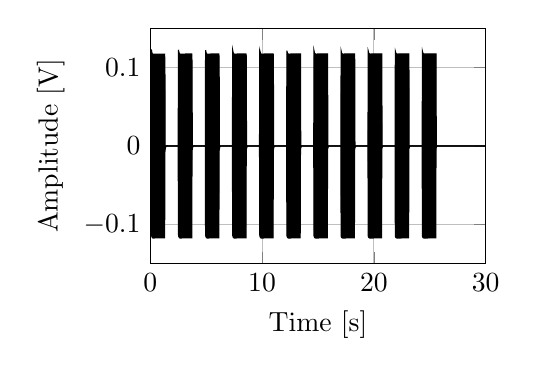
\begin{tikzpicture}

\begin{axis}[%
width=2.3in,
height=1.8in,
at={(0.758in,0.481in)},
xmin=0,
xmax=30,
xmajorgrids,
ymin=-0.15,
ymax=0.15,
ylabel={Amplitude [V]},
xlabel={Time [s]},
ymajorgrids,
axis background/.style={fill=white}
]
\addplot[fill=black,draw=black,forget plot] plot table[row sep=crcr]{%
2.08333333333333e-05	1.58548355102539e-05\\
0.0252733410493827	1.68085098266602e-05\\
0.0505258487654321	1.4185905456543e-05\\
0.0757783564814815	1.75237655639648e-05\\
0.101030864197531	0.122879505157471\\
0.12628337191358	0.120219826698303\\
0.15153587962963	0.118692755699158\\
0.176788387345679	0.117809057235718\\
0.202040895061728	0.117316246032715\\
0.227293402777778	0.117060780525208\\
0.252545910493827	0.116923570632935\\
0.277798418209877	0.116885662078857\\
0.303050925925926	0.116871953010559\\
0.328303433641975	0.11688220500946\\
0.353555941358025	0.116916537284851\\
0.378808449074074	0.116943120956421\\
0.404060956790123	0.116961240768433\\
0.429313464506173	0.116984009742737\\
0.454565972222222	0.116994857788086\\
0.479818479938272	0.11701238155365\\
0.505070987654321	0.117026567459106\\
0.53032349537037	0.117034077644348\\
0.55557600308642	0.117038011550903\\
0.580828510802469	0.117049217224121\\
0.606081018518519	0.117051243782043\\
0.631333526234568	0.117061257362366\\
0.656586033950617	0.117065787315369\\
0.681838541666667	0.117067098617554\\
0.707091049382716	0.117065906524658\\
0.732343557098765	0.117066740989685\\
0.757596064814815	0.1170734167099\\
0.782848572530864	0.117071747779846\\
0.808101080246914	0.117065906524658\\
0.833353587962963	0.117072463035584\\
0.858606095679012	0.117069125175476\\
0.883858603395062	0.117069244384766\\
0.909111111111111	0.117070555686951\\
0.934363618827161	0.11707079410553\\
0.95961612654321	0.117067933082581\\
0.984868634259259	0.117074728012085\\
1.01012114197531	0.117074131965637\\
1.03537364969136	0.117074131965637\\
1.06062615740741	0.117071390151978\\
1.08587866512346	0.117072939872742\\
1.11113117283951	0.11707079410553\\
1.13638368055556	0.117062568664551\\
1.16163618827161	0.117069959640503\\
1.18688869598765	0.117068886756897\\
1.2121412037037	0.117069125175476\\
1.23739371141975	0.11707079410553\\
1.2626462191358	0.117066621780396\\
1.28789872685185	0.117077469825745\\
1.3131512345679	0.10097062587738\\
1.33840374228395	-0.002097487449646\\
1.36365625	-0.000977039337158203\\
1.38890875771605	-0.000357866287231445\\
1.4141612654321	-3.37362289428711e-05\\
1.43941377314815	0.000129342079162598\\
1.4646662808642	0.000192880630493164\\
1.48991878858025	0.000212430953979492\\
1.5151712962963	0.000216245651245117\\
1.54042380401235	0.000203132629394531\\
1.5656763117284	0.000182390213012695\\
1.59092881944444	0.000157356262207031\\
1.61618132716049	0.000135540962219238\\
1.64143383487654	0.000110983848571777\\
1.66668634259259	9.51290130615234e-05\\
1.69193885030864	7.92741775512695e-05\\
1.71719135802469	6.47306442260742e-05\\
1.74244386574074	5.18560409545898e-05\\
1.76769637345679	4.8518180847168e-05\\
1.79294888117284	4.04119491577148e-05\\
1.81820138888889	3.20672988891602e-05\\
1.84345389660494	2.71797180175781e-05\\
1.86870640432099	2.70605087280273e-05\\
1.89395891203704	2.26497650146484e-05\\
1.91921141975309	1.96695327758789e-05\\
1.94446392746914	2.08616256713867e-05\\
1.96971643518519	1.71661376953125e-05\\
1.99496894290123	1.8000602722168e-05\\
2.02022145061728	1.38282775878906e-05\\
2.04547395833333	1.38282775878906e-05\\
2.07072646604938	1.93119049072266e-05\\
2.09597897376543	1.34706497192383e-05\\
2.12123148148148	1.43051147460938e-05\\
2.14648398919753	1.66893005371094e-05\\
2.17173649691358	1.21593475341797e-05\\
2.19698900462963	1.46627426147461e-05\\
2.22224151234568	1.43051147460938e-05\\
2.24749402006173	1.68085098266602e-05\\
2.27274652777778	1.29938125610352e-05\\
2.29799903549383	1.43051147460938e-05\\
2.32325154320988	1.50203704833984e-05\\
2.34850405092593	1.38282775878906e-05\\
2.37375655864198	1.8000602722168e-05\\
2.39900906635802	1.38282775878906e-05\\
2.42426157407407	1.53779983520508e-05\\
2.44951408179012	1.50203704833984e-05\\
2.47476658950617	1.53779983520508e-05\\
2.50001909722222	1.34706497192383e-05\\
2.52527160493827	0.122484803199768\\
2.55052411265432	0.120183825492859\\
2.57577662037037	0.118810296058655\\
2.60102912808642	0.117970824241638\\
2.62628163580247	0.11729907989502\\
2.65153414351852	0.117104768753052\\
2.67678665123457	0.116974830627441\\
2.70203915895062	0.116921067237854\\
2.72729166666667	0.116914510726929\\
2.75254417438272	0.1169353723526\\
2.77779668209877	0.116956114768982\\
2.80304918981481	0.11698317527771\\
2.82830169753086	0.116991639137268\\
2.85355420524691	0.117025017738342\\
2.87880671296296	0.117034912109375\\
2.90405922067901	0.117040872573853\\
2.92931172839506	0.11705756187439\\
2.95456423611111	0.117060780525208\\
2.97981674382716	0.117064714431763\\
3.00506925154321	0.11707592010498\\
3.03032175925926	0.117080450057983\\
3.05557426697531	0.117085814476013\\
3.08082677469136	0.117089986801147\\
3.10607928240741	0.11708927154541\\
3.13133179012346	0.117094159126282\\
3.15658429783951	0.117094993591309\\
3.18183680555556	0.117096304893494\\
3.2070893132716	0.117091774940491\\
3.23234182098765	0.117095589637756\\
3.2575943287037	0.11710250377655\\
3.28284683641975	0.117097496986389\\
3.3080993441358	0.117101430892944\\
3.33335185185185	0.117091298103333\\
3.3586043595679	0.117102146148682\\
3.38385686728395	0.117099285125732\\
3.409109375	0.117094278335571\\
3.43436188271605	0.117102265357971\\
3.4596143904321	0.117097139358521\\
3.48486689814815	0.117097973823547\\
3.5101194058642	0.117094755172729\\
3.53537191358025	0.117103934288025\\
3.5606244212963	0.117095589637756\\
3.58587692901235	0.117089748382568\\
3.61112943672839	0.117098450660706\\
3.63638194444444	0.117092490196228\\
3.66163445216049	0.117099165916443\\
3.68688695987654	0.117096662521362\\
3.71213946759259	0.117095589637756\\
3.73739197530864	0.107169151306152\\
3.76264448302469	-0.00190830230712891\\
3.78789699074074	-0.00088953971862793\\
3.81314949845679	-0.000322818756103516\\
3.83840200617284	-2.62260437011719e-05\\
3.86365451388889	0.000118494033813477\\
3.88890702160494	0.000179886817932129\\
3.91415952932099	0.000197887420654297\\
3.93941203703704	0.000200748443603516\\
3.96466454475309	0.000186920166015625\\
3.98991705246914	0.00016486644744873\\
4.01516956018518	0.000146389007568359\\
4.04042206790123	0.000122785568237305\\
4.06567457561728	0.000103473663330078\\
4.09092708333333	8.85725021362305e-05\\
4.11617959104938	7.18832015991211e-05\\
4.14143209876543	6.04391098022461e-05\\
4.16668460648148	4.92334365844727e-05\\
4.19193711419753	4.10079956054688e-05\\
4.21718962191358	3.55243682861328e-05\\
4.24244212962963	3.12328338623047e-05\\
4.26769463734568	2.58684158325195e-05\\
4.29294714506173	2.26497650146484e-05\\
4.31819965277778	2.08616256713867e-05\\
4.34345216049383	2.09808349609375e-05\\
4.36870466820988	2.00271606445313e-05\\
4.39395717592593	2.00271606445313e-05\\
4.41920968364198	1.51395797729492e-05\\
4.44446219135802	1.71661376953125e-05\\
4.46971469907407	1.8000602722168e-05\\
4.49496720679012	1.21593475341797e-05\\
4.52021971450617	1.78813934326172e-05\\
4.54547222222222	1.58548355102539e-05\\
4.57072472993827	1.59740447998047e-05\\
4.59597723765432	1.51395797729492e-05\\
4.62122974537037	1.26361846923828e-05\\
4.64648225308642	1.33514404296875e-05\\
4.67173476080247	1.29938125610352e-05\\
4.69698726851852	1.54972076416016e-05\\
4.72223977623457	1.2516975402832e-05\\
4.74749228395062	1.37090682983398e-05\\
4.77274479166667	1.62124633789063e-05\\
4.79799729938272	1.43051147460938e-05\\
4.82324980709877	1.45435333251953e-05\\
4.84850231481482	1.37090682983398e-05\\
4.87375482253086	1.59740447998047e-05\\
4.89900733024691	1.33514404296875e-05\\
4.92425983796296	1.54972076416016e-05\\
4.94951234567901	0.122136831283569\\
4.97476485339506	0.120147228240967\\
5.00001736111111	0.118440747261047\\
5.02526986882716	0.117819309234619\\
5.05052237654321	0.11729621887207\\
5.07577488425926	0.117114186286926\\
5.10102739197531	0.116984963417053\\
5.12627989969136	0.116955757141113\\
5.15153240740741	0.116954445838928\\
5.17678491512346	0.116969466209412\\
5.20203742283951	0.116990804672241\\
5.22728993055556	0.11700713634491\\
5.2525424382716	0.117026209831238\\
5.27779494598765	0.117044925689697\\
5.3030474537037	0.117066264152527\\
5.32829996141975	0.117077589035034\\
5.3535524691358	0.11708128452301\\
5.37880497685185	0.117092490196228\\
5.4040574845679	0.117095470428467\\
5.42930999228395	0.117104172706604\\
5.4545625	0.117108106613159\\
5.47981500771605	0.117108941078186\\
5.5050675154321	0.11711061000824\\
5.53032002314815	0.11711597442627\\
5.5555725308642	0.117118954658508\\
5.58082503858025	0.11712646484375\\
5.6060775462963	0.117114663124084\\
5.63133005401235	0.117119193077087\\
5.65658256172839	0.117115139961243\\
5.68183506944444	0.117118835449219\\
5.70708757716049	0.117117285728455\\
5.73234008487654	0.117123961448669\\
5.75759259259259	0.117119669914246\\
5.78284510030864	0.11712384223938\\
5.80809760802469	0.117116451263428\\
5.83335011574074	0.117116451263428\\
5.85860262345679	0.117123365402222\\
5.88385513117284	0.117119312286377\\
5.90910763888889	0.117115020751953\\
5.93436014660494	0.117121458053589\\
5.95961265432099	0.117115020751953\\
5.98486516203704	0.117119312286377\\
6.01011766975309	0.117117285728455\\
6.03537017746914	0.117118358612061\\
6.06062268518518	0.117124676704407\\
6.08587519290123	0.117120981216431\\
6.11112770061728	0.117120504379272\\
6.13638020833333	0.11711847782135\\
6.16163271604938	0.111903429031372\\
6.18688522376543	-0.00175118446350098\\
6.21213773148148	-0.00081324577331543\\
6.23739023919753	-0.000295877456665039\\
6.26264274691358	-1.8000602722168e-05\\
6.28789525462963	0.00011146068572998\\
6.31314776234568	0.00016474723815918\\
6.33840027006173	0.000183939933776855\\
6.36365277777778	0.000184059143066406\\
6.38890528549383	0.000174522399902344\\
6.41415779320988	0.000154018402099609\\
6.43941030092593	0.0001373291015625\\
6.46466280864198	0.000113487243652344\\
6.48991531635802	9.72747802734375e-05\\
6.51516782407407	7.77244567871094e-05\\
6.54042033179012	6.55651092529297e-05\\
6.56567283950617	5.80549240112305e-05\\
6.59092534722222	4.88758087158203e-05\\
6.61617785493827	4.0888786315918e-05\\
6.64143036265432	3.20672988891602e-05\\
6.66668287037037	3.00407409667969e-05\\
6.69193537808642	2.70605087280273e-05\\
6.71718788580247	2.37226486206055e-05\\
6.74244039351852	2.21729278564453e-05\\
6.76769290123457	1.96695327758789e-05\\
6.79294540895062	2.03847885131836e-05\\
6.81819791666667	1.43051147460938e-05\\
6.84345042438272	1.50203704833984e-05\\
6.86870293209877	1.66893005371094e-05\\
6.89395543981481	1.91926956176758e-05\\
6.91920794753086	1.38282775878906e-05\\
6.94446045524691	1.84774398803711e-05\\
6.96971296296296	1.62124633789063e-05\\
6.99496547067901	1.66893005371094e-05\\
7.02021797839506	1.45435333251953e-05\\
7.04547048611111	1.45435333251953e-05\\
7.07072299382716	1.51395797729492e-05\\
7.09597550154321	1.6331672668457e-05\\
7.12122800925926	1.62124633789063e-05\\
7.14648051697531	1.37090682983398e-05\\
7.17173302469136	1.38282775878906e-05\\
7.19698553240741	1.12056732177734e-05\\
7.22223804012346	1.76429748535156e-05\\
7.24749054783951	1.70469284057617e-05\\
7.27274305555556	1.83582305908203e-05\\
7.2979955632716	1.21593475341797e-05\\
7.32324807098765	1.59740447998047e-05\\
7.3485005787037	1.29938125610352e-05\\
7.37375308641975	0.12184476852417\\
7.3990055941358	0.120089888572693\\
7.42425810185185	0.1185302734375\\
7.4495106095679	0.117711305618286\\
7.47476311728395	0.117402195930481\\
7.500015625	0.117144346237183\\
7.52526813271605	0.117019653320313\\
7.5505206404321	0.116984486579895\\
7.57577314814815	0.116981267929077\\
7.6010256558642	0.116997122764587\\
7.62627816358025	0.117016196250916\\
7.6515306712963	0.11703085899353\\
7.67678317901235	0.117055416107178\\
7.70203568672839	0.117057204246521\\
7.72728819444444	0.117087960243225\\
7.75254070216049	0.117092490196228\\
7.77779320987654	0.117108941078186\\
7.80304571759259	0.117111682891846\\
7.82829822530864	0.117115616798401\\
7.85355073302469	0.117121696472168\\
7.87880324074074	0.117124199867249\\
7.90405574845679	0.117127656936646\\
7.92930825617284	0.117123961448669\\
7.95456076388889	0.117131352424622\\
7.97981327160494	0.117124319076538\\
8.00506577932099	0.117135643959045\\
8.03031828703704	0.117133140563965\\
8.05557079475309	0.117125630378723\\
8.08082330246914	0.11713171005249\\
8.10607581018519	0.117137551307678\\
8.13132831790123	0.11713981628418\\
8.15658082561728	0.117139339447021\\
8.18183333333333	0.11713981628418\\
8.20708584104938	0.117138981819153\\
8.23233834876543	0.117137670516968\\
8.25759085648148	0.117145180702209\\
8.28284336419753	0.117140054702759\\
8.30809587191358	0.117145895957947\\
8.33334837962963	0.117139220237732\\
8.35860088734568	0.117133855819702\\
8.38385339506173	0.117145657539368\\
8.40910590277778	0.117128968238831\\
8.43435841049383	0.117143392562866\\
8.45961091820988	0.117140173912048\\
8.48486342592593	0.117136478424072\\
8.51011593364198	0.117136001586914\\
8.53536844135802	0.11714231967926\\
8.56062094907407	0.117137551307678\\
8.58587345679012	0.115118741989136\\
8.61112596450617	-0.00161099433898926\\
8.63637847222222	-0.00074303150177002\\
8.66163097993827	-0.000270724296569824\\
8.68688348765432	-2.08616256713867e-05\\
8.71213599537037	0.00010216236114502\\
8.73738850308642	0.000153899192810059\\
8.76264101080247	0.000169038772583008\\
8.78789351851852	0.000168561935424805\\
8.81314602623457	0.000159859657287598\\
8.83839853395062	0.000145673751831055\\
8.86365104166667	0.000126123428344727\\
8.88890354938272	0.000107169151306152\\
8.91415605709877	9.0479850769043e-05\\
8.93940856481481	7.67707824707031e-05\\
8.96466107253086	6.43730163574219e-05\\
8.98991358024691	5.22136688232422e-05\\
9.01516608796296	4.38690185546875e-05\\
9.04041859567901	3.63588333129883e-05\\
9.06567110339506	3.20672988891602e-05\\
9.09092361111111	2.88486480712891e-05\\
9.11617611882716	2.50339508056641e-05\\
9.14142862654321	2.30073928833008e-05\\
9.16668113425926	2.13384628295898e-05\\
9.19193364197531	1.76429748535156e-05\\
9.21718614969136	2.45571136474609e-05\\
9.24243865740741	1.84774398803711e-05\\
9.26769116512346	1.62124633789063e-05\\
9.29294367283951	1.51395797729492e-05\\
9.31819618055556	1.33514404296875e-05\\
9.34344868827161	1.50203704833984e-05\\
9.36870119598765	1.53779983520508e-05\\
9.3939537037037	1.34706497192383e-05\\
9.41920621141975	1.34706497192383e-05\\
9.4444587191358	1.26361846923828e-05\\
9.46971122685185	1.51395797729492e-05\\
9.4949637345679	1.53779983520508e-05\\
9.52021624228395	1.71661376953125e-05\\
9.54546875	1.38282775878906e-05\\
9.57072125771605	1.51395797729492e-05\\
9.5959737654321	1.62124633789063e-05\\
9.62122627314815	1.54972076416016e-05\\
9.6464787808642	1.59740447998047e-05\\
9.67173128858025	1.58548355102539e-05\\
9.6969837962963	1.54972076416016e-05\\
9.72223630401235	1.76429748535156e-05\\
9.7474888117284	1.29938125610352e-05\\
9.77274131944444	1.84774398803711e-05\\
9.79799382716049	0.121572375297546\\
9.82324633487654	0.120015263557434\\
9.84849884259259	0.118595480918884\\
9.87375135030864	0.117800235748291\\
9.89900385802469	0.117379188537598\\
9.92425636574074	0.117158889770508\\
9.94950887345679	0.11705470085144\\
9.97476138117284	0.117006659507751\\
10.0000138888889	0.117013812065125\\
10.0252663966049	0.117024898529053\\
10.050518904321	0.11704421043396\\
10.075771412037	0.117059230804443\\
10.1010239197531	0.117070555686951\\
10.1262764274691	0.117085576057434\\
10.1515289351852	0.117094159126282\\
10.1767814429012	0.117107629776001\\
10.2020339506173	0.117117285728455\\
10.2272864583333	0.117114663124084\\
10.2525389660494	0.117132663726807\\
10.2777914737654	0.117130637168884\\
10.3030439814815	0.117143034934998\\
10.3282964891975	0.117150545120239\\
10.3535489969136	0.117147207260132\\
10.3788015046296	0.117142677307129\\
10.4040540123457	0.117141008377075\\
10.4293065200617	0.117145657539368\\
10.4545590277778	0.117155909538269\\
10.4798115354938	0.117148160934448\\
10.5050640432099	0.117153406143188\\
10.5303165509259	0.117146730422974\\
10.555569058642	0.117155194282532\\
10.580821566358	0.117154240608215\\
10.6060740740741	0.117156505584717\\
10.6313265817901	0.117158889770508\\
10.6565790895062	0.117149710655212\\
10.6818315972222	0.117150664329529\\
10.7070841049383	0.117155075073242\\
10.7323366126543	0.117151737213135\\
10.7575891203704	0.117151379585266\\
10.7828416280864	0.117152571678162\\
10.8080941358025	0.117152333259583\\
10.8333466435185	0.11715304851532\\
10.8585991512346	0.117153167724609\\
10.8838516589506	0.11715304851532\\
10.9091041666667	0.117150545120239\\
10.9343566743827	0.117151021957397\\
10.9596091820988	0.117149233818054\\
10.9848616898148	0.117151856422424\\
11.0101141975309	0.116843819618225\\
11.0353667052469	-0.00150108337402344\\
11.060619212963	-0.000692605972290039\\
11.085871720679	-0.000258207321166992\\
11.1111242283951	-1.95503234863281e-05\\
11.1363767361111	9.22679901123047e-05\\
11.1616292438272	0.000141143798828125\\
11.1868817515432	0.000156521797180176\\
11.2121342592593	0.000157713890075684\\
11.2373867669753	0.000151872634887695\\
11.2626392746914	0.000136852264404297\\
11.2878917824074	0.000113487243652344\\
11.3131442901235	9.94205474853516e-05\\
11.3383967978395	9.10758972167969e-05\\
11.3636493055556	7.02142715454102e-05\\
11.3889018132716	5.93662261962891e-05\\
11.4141543209877	5.68628311157227e-05\\
11.4394068287037	4.20808792114258e-05\\
11.4646593364198	3.83853912353516e-05\\
11.4899118441358	3.30209732055664e-05\\
11.5151643518519	2.58684158325195e-05\\
11.5404168595679	2.37226486206055e-05\\
11.565669367284	2.41994857788086e-05\\
11.590921875	2.21729278564453e-05\\
11.6161743827161	1.96695327758789e-05\\
11.6414268904321	1.70469284057617e-05\\
11.6666793981481	1.93119049072266e-05\\
11.6919319058642	1.8000602722168e-05\\
11.7171844135802	2.00271606445313e-05\\
11.7424369212963	1.6331672668457e-05\\
11.7676894290123	1.62124633789063e-05\\
11.7929419367284	1.68085098266602e-05\\
11.8181944444444	1.6331672668457e-05\\
11.8434469521605	1.46627426147461e-05\\
11.8686994598765	1.75237655639648e-05\\
11.8939519675926	1.29938125610352e-05\\
11.9192044753086	1.33514404296875e-05\\
11.9444569830247	1.59740447998047e-05\\
11.9697094907407	1.6331672668457e-05\\
11.9949619984568	1.38282775878906e-05\\
12.0202145061728	1.28746032714844e-05\\
12.0454670138889	1.6331672668457e-05\\
12.0707195216049	1.71661376953125e-05\\
12.095972029321	1.38282775878906e-05\\
12.121224537037	1.37090682983398e-05\\
12.1464770447531	1.58548355102539e-05\\
12.1717295524691	2.00271606445313e-05\\
12.1969820601852	1.51395797729492e-05\\
12.2222345679012	0.121322989463806\\
12.2474870756173	0.119430780410767\\
12.2727395833333	0.118337512016296\\
12.2979920910494	0.117706418037415\\
12.3232445987654	0.117356300354004\\
12.3484971064815	0.117170214653015\\
12.3737496141975	0.117075443267822\\
12.3990021219136	0.117034077644348\\
12.4242546296296	0.117026567459106\\
12.4495071373457	0.117044925689697\\
12.4747596450617	0.117059230804443\\
12.5000121527778	0.117071628570557\\
12.5252646604938	0.117092967033386\\
12.5505171682099	0.11710512638092\\
12.5757696759259	0.11711061000824\\
12.601022183642	0.11711311340332\\
12.626274691358	0.117130517959595\\
12.6515271990741	0.11713719367981\\
12.6767797067901	0.117137312889099\\
12.7020322145062	0.117154717445374\\
12.7272847222222	0.11714768409729\\
12.7525372299383	0.117150068283081\\
12.7777897376543	0.117154836654663\\
12.8030422453704	0.117156863212585\\
12.8282947530864	0.117158055305481\\
12.8535472608025	0.117160201072693\\
12.8787997685185	0.117162346839905\\
12.9040522762346	0.11716103553772\\
12.9293047839506	0.11715841293335\\
12.9545572916667	0.117161393165588\\
12.9798097993827	0.117159247398376\\
13.0050623070988	0.117155909538269\\
13.0303148148148	0.117157340049744\\
13.0555673225309	0.117167353630066\\
13.0808198302469	0.117165088653564\\
13.106072337963	0.117163062095642\\
13.131324845679	0.117162704467773\\
13.1565773533951	0.117162704467773\\
13.1818298611111	0.117157697677612\\
13.2070823688272	0.117157697677612\\
13.2323348765432	0.11716103553772\\
13.2575873842593	0.117165923118591\\
13.2828398919753	0.117160677909851\\
13.3080923996914	0.117161750793457\\
13.3333449074074	0.117158889770508\\
13.3585974151235	0.117161512374878\\
13.3838499228395	0.1171635389328\\
13.4091024305556	0.117165565490723\\
13.4343549382716	0.117153167724609\\
13.4596074459877	-0.0013965368270874\\
13.4848599537037	-0.000646233558654785\\
13.5101124614198	-0.000239133834838867\\
13.5353649691358	-1.95503234863281e-05\\
13.5606174768519	9.13143157958984e-05\\
13.5858699845679	0.000134706497192383\\
13.611122492284	0.000146031379699707\\
13.636375	0.000151395797729492\\
13.6616275077161	0.000142693519592285\\
13.6868800154321	0.000128626823425293\\
13.7121325231481	0.000111937522888184\\
13.7373850308642	9.6440315246582e-05\\
13.7626375385802	8.13007354736328e-05\\
13.7878900462963	6.68764114379883e-05\\
13.8131425540123	5.68628311157227e-05\\
13.8383950617284	4.76837158203125e-05\\
13.8636475694444	3.93390655517578e-05\\
13.8889000771605	3.4332275390625e-05\\
13.9141525848765	3.29017639160156e-05\\
13.9394050925926	2.76565551757813e-05\\
13.9646576003086	2.63452529907227e-05\\
13.9899101080247	2.03847885131836e-05\\
14.0151626157407	2.09808349609375e-05\\
14.0404151234568	2.0146369934082e-05\\
14.0656676311728	1.84774398803711e-05\\
14.0909201388889	1.54972076416016e-05\\
14.1161726466049	1.54972076416016e-05\\
14.141425154321	1.28746032714844e-05\\
14.166677662037	1.68085098266602e-05\\
14.1919301697531	1.50203704833984e-05\\
14.2171826774691	1.43051147460938e-05\\
14.2424351851852	1.34706497192383e-05\\
14.2676876929012	1.21593475341797e-05\\
14.2929402006173	1.54972076416016e-05\\
14.3181927083333	1.51395797729492e-05\\
14.3434452160494	1.95503234863281e-05\\
14.3686977237654	1.83582305908203e-05\\
14.3939502314815	1.37090682983398e-05\\
14.4192027391975	1.84774398803711e-05\\
14.4444552469136	1.87158584594727e-05\\
14.4697077546296	1.54972076416016e-05\\
14.4949602623457	1.4185905456543e-05\\
14.5202127700617	1.51395797729492e-05\\
14.5454652777778	1.66893005371094e-05\\
14.5707177854938	1.4185905456543e-05\\
14.5959702932099	1.54972076416016e-05\\
14.6212228009259	1.37090682983398e-05\\
14.646475308642	0.121119737625122\\
14.671727816358	0.119396567344666\\
14.6969803240741	0.11837899684906\\
14.7222328317901	0.117777705192566\\
14.7474853395062	0.117345333099365\\
14.7727378472222	0.117175102233887\\
14.7979903549383	0.117093920707703\\
14.8232428626543	0.117048859596252\\
14.8484953703704	0.117047071456909\\
14.8737478780864	0.117058277130127\\
14.8990003858025	0.117074608802795\\
14.9242528935185	0.117087244987488\\
14.9495054012346	0.117104649543762\\
14.9747579089506	0.117116332054138\\
15.0000104166667	0.11712384223938\\
15.0252629243827	0.117133021354675\\
15.0505154320988	0.11713981628418\\
15.0757679398148	0.117148160934448\\
15.1010204475309	0.117156505584717\\
15.1262729552469	0.117164254188538\\
15.151525462963	0.11716091632843\\
15.176777970679	0.117161750793457\\
15.2020304783951	0.117171049118042\\
15.2272829861111	0.117166519165039\\
15.2525354938272	0.117164015769959\\
15.2777880015432	0.117171049118042\\
15.3030405092593	0.117171764373779\\
15.3282930169753	0.117170691490173\\
15.3535455246914	0.117169380187988\\
15.3787980324074	0.117179274559021\\
15.4040505401235	0.117166757583618\\
15.4293030478395	0.117171049118042\\
15.4545555555556	0.117173075675964\\
15.4798080632716	0.117171049118042\\
15.5050605709877	0.117173194885254\\
15.5303130787037	0.117174744606018\\
15.5555655864198	0.117173433303833\\
15.5808180941358	0.117167592048645\\
15.6060706018519	0.117179393768311\\
15.6313231095679	0.117175579071045\\
15.656575617284	0.117165207862854\\
15.681828125	0.117167353630066\\
15.7070806327161	0.117172241210938\\
15.7323331404321	0.117172360420227\\
15.7575856481481	0.117165684700012\\
15.7828381558642	0.117171883583069\\
15.8080906635802	0.117170095443726\\
15.8333431712963	0.117170929908752\\
15.8585956790123	0.117159366607666\\
15.8838481867284	-0.00130629539489746\\
15.9091006944444	-0.000602126121520996\\
15.9343532021605	-0.00022435188293457\\
15.9596057098765	-1.58548355102539e-05\\
15.9848582175926	8.30888748168945e-05\\
16.0101107253086	0.000125527381896973\\
16.0353632330247	0.000137686729431152\\
16.0606157407407	0.000142335891723633\\
16.0858682484568	0.000131964683532715\\
16.1111207561728	0.000119805335998535\\
16.1363732638889	0.000101089477539063\\
16.1616257716049	9.02414321899414e-05\\
16.186878279321	7.43865966796875e-05\\
16.212130787037	6.46114349365234e-05\\
16.2373832947531	5.60283660888672e-05\\
16.2626358024691	4.8518180847168e-05\\
16.2878883101852	4.18424606323242e-05\\
16.3131408179012	3.38554382324219e-05\\
16.3383933256173	3.08752059936523e-05\\
16.3636458333333	2.53915786743164e-05\\
16.3888983410494	2.45571136474609e-05\\
16.4141508487654	2.46763229370117e-05\\
16.4394033564815	1.96695327758789e-05\\
16.4646558641975	1.8000602722168e-05\\
16.4899083719136	1.70469284057617e-05\\
16.5151608796296	1.62124633789063e-05\\
16.5404133873457	2.16960906982422e-05\\
16.5656658950617	1.50203704833984e-05\\
16.5909184027778	2.16960906982422e-05\\
16.6161709104938	1.33514404296875e-05\\
16.6414234182099	1.68085098266602e-05\\
16.6666759259259	1.51395797729492e-05\\
16.691928433642	1.51395797729492e-05\\
16.717180941358	1.59740447998047e-05\\
16.7424334490741	1.43051147460938e-05\\
16.7676859567901	1.46627426147461e-05\\
16.7929384645062	1.46627426147461e-05\\
16.8181909722222	1.59740447998047e-05\\
16.8434434799383	1.6331672668457e-05\\
16.8686959876543	1.84774398803711e-05\\
16.8939484953704	1.59740447998047e-05\\
16.9192010030864	1.95503234863281e-05\\
16.9444535108025	1.71661376953125e-05\\
16.9697060185185	1.50203704833984e-05\\
16.9949585262346	1.50203704833984e-05\\
17.0202110339506	1.43051147460938e-05\\
17.0454635416667	1.59740447998047e-05\\
17.0707160493827	0.120926856994629\\
17.0959685570988	0.119378209114075\\
17.1212210648148	0.118203639984131\\
17.1464735725309	0.117694973945618\\
17.1717260802469	0.117335319519043\\
17.196978587963	0.117192268371582\\
17.222231095679	0.117097616195679\\
17.2474836033951	0.117066740989685\\
17.2727361111111	0.11705756187439\\
17.2979886188272	0.1170654296875\\
17.3232411265432	0.117082476615906\\
17.3484936342593	0.117109179496765\\
17.3737461419753	0.117106676101685\\
17.3989986496914	0.117122173309326\\
17.4242511574074	0.117138981819153\\
17.4495036651235	0.117141842842102\\
17.4747561728395	0.117156863212585\\
17.5000086805556	0.117157340049744\\
17.5252611882716	0.117165088653564\\
17.5505136959877	0.117173194885254\\
17.5757662037037	0.117165088653564\\
17.6010187114198	0.117175698280334\\
17.6262712191358	0.117171883583069\\
17.6515237268519	0.117169857025146\\
17.6767762345679	0.117180228233337\\
17.702028742284	0.117179036140442\\
17.72728125	0.117185115814209\\
17.7525337577161	0.117179036140442\\
17.7777862654321	0.117178201675415\\
17.8030387731481	0.117188215255737\\
17.8282912808642	0.11717689037323\\
17.8535437885803	0.117181420326233\\
17.8787962962963	0.117181420326233\\
17.9040488040123	0.117183208465576\\
17.9293013117284	0.11718487739563\\
17.9545538194444	0.117179036140442\\
17.9798063271605	0.117180943489075\\
18.0050588348765	0.117177724838257\\
18.0303113425926	0.117183923721313\\
18.0555638503086	0.117178440093994\\
18.0808163580247	0.117181062698364\\
18.1060688657407	0.117178916931152\\
18.1313213734568	0.117185592651367\\
18.1565738811728	0.117179751396179\\
18.1818263888889	0.117183208465576\\
18.2070788966049	0.117183208465576\\
18.232331404321	0.117177605628967\\
18.257583912037	0.117175698280334\\
18.2828364197531	0.117178916931152\\
18.3080889274691	-0.00123071670532227\\
18.3333414351852	-0.000575661659240723\\
18.3585939429012	-0.000205278396606445\\
18.3838464506173	-1.95503234863281e-05\\
18.4090989583333	7.77244567871094e-05\\
18.4343514660494	0.000117778778076172\\
18.4596039737654	0.000131130218505859\\
18.4848564814815	0.000134706497192383\\
18.5101089891975	0.000125527381896973\\
18.5353614969136	0.000114679336547852\\
18.5606140046296	0.000100970268249512\\
18.5858665123457	8.67843627929688e-05\\
18.6111190200617	7.93933868408203e-05\\
18.6363715277778	6.27040863037109e-05\\
18.6616240354938	5.00679016113281e-05\\
18.6868765432099	4.55379486083984e-05\\
18.7121290509259	3.88622283935547e-05\\
18.737381558642	3.17096710205078e-05\\
18.762634066358	2.83718109130859e-05\\
18.7878865740741	2.50339508056641e-05\\
18.8131390817901	2.55107879638672e-05\\
18.8383915895062	2.08616256713867e-05\\
18.8636440972222	1.96695327758789e-05\\
18.8888966049383	2.26497650146484e-05\\
18.9141491126543	1.6331672668457e-05\\
18.9394016203704	1.6331672668457e-05\\
18.9646541280864	1.91926956176758e-05\\
18.9899066358025	1.38282775878906e-05\\
19.0151591435185	1.4185905456543e-05\\
19.0404116512346	1.6331672668457e-05\\
19.0656641589506	1.59740447998047e-05\\
19.0909166666667	1.54972076416016e-05\\
19.1161691743827	1.43051147460938e-05\\
19.1414216820988	1.58548355102539e-05\\
19.1666741898148	1.38282775878906e-05\\
19.1919266975309	1.4185905456543e-05\\
19.2171792052469	1.45435333251953e-05\\
19.242431712963	1.29938125610352e-05\\
19.267684220679	1.51395797729492e-05\\
19.2929367283951	1.2516975402832e-05\\
19.3181892361111	1.6331672668457e-05\\
19.3434417438272	1.43051147460938e-05\\
19.3686942515432	1.54972076416016e-05\\
19.3939467592593	1.45435333251953e-05\\
19.4191992669753	1.91926956176758e-05\\
19.4444517746914	1.46627426147461e-05\\
19.4697042824074	1.50203704833984e-05\\
19.4949567901235	0.120749235153198\\
19.5202092978395	0.119339823722839\\
19.5454618055556	0.11822497844696\\
19.5707143132716	0.117634654045105\\
19.5959668209877	0.117380023002625\\
19.6212193287037	0.117199420928955\\
19.6464718364198	0.117104649543762\\
19.6717243441358	0.117072939872742\\
19.6969768518519	0.117077469825745\\
19.7222293595679	0.117088317871094\\
19.747481867284	0.117100834846497\\
19.772734375	0.11710250377655\\
19.797986882716	0.117123484611511\\
19.8232393904321	0.117137312889099\\
19.8484918981482	0.117151379585266\\
19.8737444058642	0.117156386375427\\
19.8989969135802	0.117152690887451\\
19.9242494212963	0.117169737815857\\
19.9495019290123	0.117164373397827\\
19.9747544367284	0.117177248001099\\
20.0000069444444	0.117178916931152\\
20.0252594521605	0.117188096046448\\
20.0505119598765	0.11718487739563\\
20.0757644675926	0.117183446884155\\
20.1010169753086	0.117179036140442\\
20.1262694830247	0.117183208465576\\
20.1515219907407	0.117185711860657\\
20.1767744984568	0.117181539535522\\
20.2020270061728	0.117182374000549\\
20.2272795138889	0.117188215255737\\
20.2525320216049	0.117190599441528\\
20.277784529321	0.117191076278687\\
20.303037037037	0.117186903953552\\
20.3282895447531	0.117191076278687\\
20.3535420524691	0.11718475818634\\
20.3787945601852	0.117183089256287\\
20.4040470679012	0.117189407348633\\
20.4292995756173	0.117185592651367\\
20.4545520833333	0.117185592651367\\
20.4798045910494	0.117187738418579\\
20.5050570987654	0.117182731628418\\
20.5303096064815	0.117193102836609\\
20.5555621141975	0.117186784744263\\
20.5808146219136	0.117185711860657\\
20.6060671296296	0.117184281349182\\
20.6313196373457	0.11718487739563\\
20.6565721450617	0.117187261581421\\
20.6818246527778	0.117189764976501\\
20.7070771604938	0.117178916931152\\
20.7323296682099	-0.00116312503814697\\
20.7575821759259	-0.000541448593139648\\
20.782834683642	-0.00019681453704834\\
20.808087191358	-1.38282775878906e-05\\
20.8333396990741	7.64131546020508e-05\\
20.8585922067901	0.000113129615783691\\
20.8838447145062	0.000133037567138672\\
20.9090972222222	0.000124454498291016\\
20.9343497299383	0.000122189521789551\\
20.9596022376543	0.000113964080810547\\
20.9848547453704	9.21487808227539e-05\\
21.0101072530864	8.13007354736328e-05\\
21.0353597608025	6.79492950439453e-05\\
21.0606122685185	5.97238540649414e-05\\
21.0858647762346	5.17368316650391e-05\\
21.1111172839506	4.20808792114258e-05\\
21.1363697916667	3.83853912353516e-05\\
21.1616222993827	3.33786010742188e-05\\
21.1868748070988	2.76565551757813e-05\\
21.2121273148148	2.55107879638672e-05\\
21.2373798225309	2.20537185668945e-05\\
21.2626323302469	2.0146369934082e-05\\
21.287884837963	1.75237655639648e-05\\
21.313137345679	1.70469284057617e-05\\
21.3383898533951	1.87158584594727e-05\\
21.3636423611111	1.59740447998047e-05\\
21.3888948688272	1.50203704833984e-05\\
21.4141473765432	2.26497650146484e-05\\
21.4393998842593	1.58548355102539e-05\\
21.4646523919753	1.59740447998047e-05\\
21.4899048996914	1.8000602722168e-05\\
21.5151574074074	1.37090682983398e-05\\
21.5404099151235	1.33514404296875e-05\\
21.5656624228395	1.71661376953125e-05\\
21.5909149305556	1.59740447998047e-05\\
21.6161674382716	1.43051147460938e-05\\
21.6414199459877	1.58548355102539e-05\\
21.6666724537037	1.54972076416016e-05\\
21.6919249614198	1.46627426147461e-05\\
21.7171774691358	1.6331672668457e-05\\
21.7424299768519	1.54972076416016e-05\\
21.7676824845679	1.59740447998047e-05\\
21.792934992284	1.53779983520508e-05\\
21.8181875	1.46627426147461e-05\\
21.8434400077161	1.58548355102539e-05\\
21.8686925154321	1.88350677490234e-05\\
21.8939450231481	1.58548355102539e-05\\
21.9191975308642	0.120596170425415\\
21.9444500385803	0.119302153587341\\
21.9697025462963	0.118262887001038\\
21.9949550540123	0.117682576179504\\
22.0202075617284	0.117359280586243\\
22.0454600694444	0.117203950881958\\
22.0707125771605	0.117124319076538\\
22.0959650848765	0.117083430290222\\
22.1212175925926	0.117083787918091\\
22.1464701003086	0.117091298103333\\
22.1717226080247	0.11711061000824\\
22.1969751157407	0.117120146751404\\
22.2222276234568	0.117133498191834\\
22.2474801311728	0.11713969707489\\
22.2727326388889	0.117153167724609\\
22.2979851466049	0.117171049118042\\
22.323237654321	0.117168068885803\\
22.348490162037	0.117171049118042\\
22.3737426697531	0.117175102233887\\
22.3989951774691	0.117181539535522\\
22.4242476851852	0.117188453674316\\
22.4495001929012	0.117183089256287\\
22.4747527006173	0.117186546325684\\
22.5000052083333	0.11718225479126\\
22.5252577160494	0.117189288139343\\
22.5505102237654	0.117201447486877\\
22.5757627314815	0.117195129394531\\
22.6010152391975	0.117189049720764\\
22.6262677469136	0.117189407348633\\
22.6515202546296	0.117195129394531\\
22.6767727623457	0.117196083068848\\
22.7020252700617	0.117192625999451\\
22.7272777777778	0.117191791534424\\
22.7525302854938	0.117183923721313\\
22.7777827932099	0.117191076278687\\
22.8030353009259	0.117192625999451\\
22.828287808642	0.117190718650818\\
22.853540316358	0.117193937301636\\
22.8787928240741	0.117192268371582\\
22.9040453317901	0.117197394371033\\
22.9292978395062	0.117189764976501\\
22.9545503472222	0.117191076278687\\
22.9798028549383	0.117191910743713\\
23.0050553626543	0.117190718650818\\
23.0303078703704	0.117206454277039\\
23.0555603780864	0.117193937301636\\
23.0808128858025	0.117188215255737\\
23.1060653935185	0.117187261581421\\
23.1313179012346	0.117185950279236\\
23.1565704089506	-0.00110018253326416\\
23.1818229166667	-0.000504493713378906\\
23.2070754243827	-0.000182390213012695\\
23.2323279320988	-1.07288360595703e-05\\
23.2575804398148	7.00950622558594e-05\\
23.2828329475309	0.000109672546386719\\
23.3080854552469	0.000119686126708984\\
23.333337962963	0.000123143196105957\\
23.358590470679	0.000113606452941895\\
23.3838429783951	0.000101923942565918\\
23.4090954861111	9.19103622436523e-05\\
23.4343479938272	7.77244567871094e-05\\
23.4596005015432	6.52074813842773e-05\\
23.4848530092593	6.05583190917969e-05\\
23.5101055169753	5.04255294799805e-05\\
23.5353580246914	4.22000885009766e-05\\
23.5606105324074	3.45706939697266e-05\\
23.5858630401235	3.13520431518555e-05\\
23.6111155478395	2.62260437011719e-05\\
23.6363680555556	2.288818359375e-05\\
23.6616205632716	2.21729278564453e-05\\
23.6868730709877	2.53915786743164e-05\\
23.7121255787037	1.87158584594727e-05\\
23.7373780864198	1.8000602722168e-05\\
23.7626305941358	2.20537185668945e-05\\
23.7878831018519	1.71661376953125e-05\\
23.8131356095679	1.87158584594727e-05\\
23.838388117284	1.68085098266602e-05\\
23.863640625	1.50203704833984e-05\\
23.888893132716	1.37090682983398e-05\\
23.9141456404321	1.59740447998047e-05\\
23.9393981481482	1.38282775878906e-05\\
23.9646506558642	1.8000602722168e-05\\
23.9899031635802	1.4185905456543e-05\\
24.0151556712963	1.6331672668457e-05\\
24.0404081790123	1.43051147460938e-05\\
24.0656606867284	1.76429748535156e-05\\
24.0909131944444	1.43051147460938e-05\\
24.1161657021605	1.33514404296875e-05\\
24.1414182098765	1.75237655639648e-05\\
24.1666707175926	1.62124633789063e-05\\
24.1919232253086	1.51395797729492e-05\\
24.2171757330247	2.00271606445313e-05\\
24.2424282407407	1.66893005371094e-05\\
24.2676807484568	1.75237655639648e-05\\
24.2929332561728	1.38282775878906e-05\\
24.3181857638889	1.62124633789063e-05\\
24.3434382716049	0.12043833732605\\
24.368690779321	0.118965148925781\\
24.393943287037	0.118106365203857\\
24.4191957947531	0.117617845535278\\
24.4444483024691	0.117347836494446\\
24.4697008101852	0.11720860004425\\
24.4949533179012	0.117131352424622\\
24.5202058256173	0.117092490196228\\
24.5454583333333	0.117092490196228\\
24.5707108410494	0.117101430892944\\
24.5959633487654	0.117108345031738\\
24.6212158564815	0.117124795913696\\
24.6464683641975	0.117135047912598\\
24.6717208719136	0.117146372795105\\
24.6969733796296	0.1171555519104\\
24.7222258873457	0.117163419723511\\
24.7474783950617	0.117166876792908\\
24.7727309027778	0.11717677116394\\
24.7979834104938	0.117181062698364\\
24.8232359182099	0.117178559303284\\
24.8484884259259	0.117177367210388\\
24.873740933642	0.117191076278687\\
24.898993441358	0.117182374000549\\
24.9242459490741	0.117188096046448\\
24.9494984567901	0.117188215255737\\
24.9747509645062	0.117191433906555\\
25.0000034722222	0.117191791534424\\
25.0252559799383	0.117189884185791\\
25.0505084876543	0.117188930511475\\
25.0757609953704	0.117192387580872\\
25.1010135030864	0.117194890975952\\
25.1262660108025	0.117196440696716\\
25.1515185185185	0.117193102836609\\
25.1767710262346	0.117185950279236\\
25.2020235339506	0.117194771766663\\
25.2272760416667	0.117188453674316\\
25.2525285493827	0.11719810962677\\
25.2777810570988	0.117190718650818\\
25.3030335648148	0.117195248603821\\
25.3282860725309	0.117193222045898\\
25.3535385802469	0.117190957069397\\
25.378791087963	0.117193579673767\\
25.404043595679	0.117189049720764\\
25.4292961033951	0.117193937301636\\
25.4545486111111	0.11718761920929\\
25.4798011188272	0.117189288139343\\
25.5050536265432	0.117192268371582\\
25.5303061342593	0.117191433906555\\
25.5555586419753	0.117186069488525\\
25.5808111496914	-0.00104260444641113\\
25.6060636574074	-0.000486850738525391\\
25.6313161651235	-0.000173211097717285\\
25.6565686728395	-1.40666961669922e-05\\
25.6818211805556	6.63995742797852e-05\\
25.7070736882716	0.000101447105407715\\
25.7323261959877	0.000113844871520996\\
25.7575787037037	0.000117182731628418\\
25.7828312114198	0.000109672546386719\\
25.8080837191358	9.71555709838867e-05\\
25.8333362268519	8.71419906616211e-05\\
25.8585887345679	7.22408294677734e-05\\
25.883841242284	6.3776969909668e-05\\
25.90909375	5.51939010620117e-05\\
25.9343462577161	4.63724136352539e-05\\
25.9595987654321	4.00543212890625e-05\\
25.9848512731481	3.50475311279297e-05\\
26.0101037808642	3.21865081787109e-05\\
26.0353562885803	2.70605087280273e-05\\
26.0606087962963	2.33650207519531e-05\\
26.0858613040123	2.33650207519531e-05\\
26.1111138117284	2.20537185668945e-05\\
26.1363663194444	1.96695327758789e-05\\
26.1616188271605	1.75237655639648e-05\\
26.1868713348765	1.8000602722168e-05\\
26.2121238425926	1.59740447998047e-05\\
26.2373763503086	1.46627426147461e-05\\
26.2626288580247	1.59740447998047e-05\\
26.2878813657407	1.83582305908203e-05\\
26.3131338734568	1.6331672668457e-05\\
26.3383863811728	1.58548355102539e-05\\
26.3636388888889	1.51395797729492e-05\\
26.3888913966049	1.75237655639648e-05\\
26.414143904321	1.43051147460938e-05\\
26.439396412037	1.8000602722168e-05\\
26.4646489197531	1.59740447998047e-05\\
26.4899014274691	1.38282775878906e-05\\
26.5151539351852	1.45435333251953e-05\\
26.5404064429012	1.62124633789063e-05\\
26.5656589506173	1.33514404296875e-05\\
26.5909114583333	1.59740447998047e-05\\
26.6161639660494	1.84774398803711e-05\\
26.6414164737654	1.6331672668457e-05\\
26.6666689814815	1.71661376953125e-05\\
26.6919214891975	1.53779983520508e-05\\
26.7171739969136	1.75237655639648e-05\\
26.7424265046296	1.54972076416016e-05\\
26.7676790123457	1.58548355102539e-05\\
26.7929315200617	1.43051147460938e-05\\
26.8181840277778	1.87158584594727e-05\\
26.8434365354938	1.6331672668457e-05\\
26.8686890432099	1.88350677490234e-05\\
26.8939415509259	1.75237655639648e-05\\
26.919194058642	1.8000602722168e-05\\
26.944446566358	1.68085098266602e-05\\
26.9696990740741	1.71661376953125e-05\\
26.9949515817901	1.6331672668457e-05\\
27.0202040895062	1.6331672668457e-05\\
27.0454565972222	1.66893005371094e-05\\
27.0707091049383	1.51395797729492e-05\\
27.0959616126543	1.88350677490234e-05\\
27.1212141203704	1.37090682983398e-05\\
27.1464666280864	1.54972076416016e-05\\
27.1717191358025	1.28746032714844e-05\\
27.1969716435185	1.58548355102539e-05\\
27.2222241512346	1.54972076416016e-05\\
27.2474766589506	1.66893005371094e-05\\
27.2727291666667	1.71661376953125e-05\\
27.2979816743827	1.58548355102539e-05\\
27.3232341820988	1.45435333251953e-05\\
27.3484866898148	1.59740447998047e-05\\
27.3737391975309	1.6331672668457e-05\\
27.3989917052469	1.46627426147461e-05\\
27.424244212963	1.87158584594727e-05\\
27.449496720679	1.75237655639648e-05\\
27.4747492283951	1.95503234863281e-05\\
27.5000017361111	1.58548355102539e-05\\
27.5252542438272	1.58548355102539e-05\\
27.5505067515432	1.70469284057617e-05\\
27.5757592592593	1.58548355102539e-05\\
27.6010117669753	1.53779983520508e-05\\
27.6262642746914	1.66893005371094e-05\\
27.6515167824074	1.88350677490234e-05\\
27.6767692901235	1.91926956176758e-05\\
27.7020217978395	1.59740447998047e-05\\
27.7272743055556	1.66893005371094e-05\\
27.7525268132716	1.78813934326172e-05\\
27.7777793209877	1.66893005371094e-05\\
27.8030318287037	1.37090682983398e-05\\
27.8282843364198	1.6331672668457e-05\\
27.8535368441358	1.4185905456543e-05\\
27.8787893518519	1.75237655639648e-05\\
27.9040418595679	1.88350677490234e-05\\
27.929294367284	1.68085098266602e-05\\
27.954546875	1.53779983520508e-05\\
27.979799382716	1.93119049072266e-05\\
28.0050518904321	1.8000602722168e-05\\
28.0303043981482	1.53779983520508e-05\\
28.0555569058642	2.16960906982422e-05\\
28.0808094135802	2.13384628295898e-05\\
28.1060619212963	1.68085098266602e-05\\
28.1313144290123	1.43051147460938e-05\\
28.1565669367284	1.54972076416016e-05\\
28.1818194444444	1.58548355102539e-05\\
28.2070719521605	1.68085098266602e-05\\
28.2323244598765	1.76429748535156e-05\\
28.2575769675926	1.59740447998047e-05\\
28.2828294753086	1.87158584594727e-05\\
28.3080819830247	1.6331672668457e-05\\
28.3333344907407	1.75237655639648e-05\\
28.3585869984568	1.51395797729492e-05\\
28.3838395061728	1.4185905456543e-05\\
28.4090920138889	1.51395797729492e-05\\
28.4343445216049	1.76429748535156e-05\\
28.459597029321	1.51395797729492e-05\\
28.484849537037	1.71661376953125e-05\\
28.5101020447531	1.88350677490234e-05\\
28.5353545524691	1.68085098266602e-05\\
28.5606070601852	1.6331672668457e-05\\
28.5858595679012	1.78813934326172e-05\\
28.6111120756173	1.6331672668457e-05\\
28.6363645833333	1.71661376953125e-05\\
28.6616170910494	1.88350677490234e-05\\
28.6868695987654	1.71661376953125e-05\\
28.7121221064815	1.71661376953125e-05\\
28.7373746141975	1.8000602722168e-05\\
28.7626271219136	1.62124633789063e-05\\
28.7878796296296	1.75237655639648e-05\\
28.8131321373457	1.76429748535156e-05\\
28.8383846450617	1.75237655639648e-05\\
28.8636371527778	1.6331672668457e-05\\
28.8888896604938	1.70469284057617e-05\\
28.9141421682099	1.70469284057617e-05\\
28.9393946759259	2.03847885131836e-05\\
28.964647183642	1.87158584594727e-05\\
28.989899691358	1.76429748535156e-05\\
29.0151521990741	1.53779983520508e-05\\
29.0404047067901	1.68085098266602e-05\\
29.0656572145062	2.00271606445313e-05\\
29.0909097222222	1.68085098266602e-05\\
29.1161622299383	1.70469284057617e-05\\
29.1414147376543	1.50203704833984e-05\\
29.1666672453704	1.84774398803711e-05\\
29.1919197530864	1.66893005371094e-05\\
29.2171722608025	1.76429748535156e-05\\
29.2424247685185	1.53779983520508e-05\\
29.2676772762346	1.43051147460938e-05\\
29.2929297839506	1.6331672668457e-05\\
29.3181822916667	1.71661376953125e-05\\
29.3434347993827	1.95503234863281e-05\\
29.3686873070988	1.58548355102539e-05\\
29.3939398148148	2.00271606445313e-05\\
29.4191923225309	1.43051147460938e-05\\
29.4444448302469	1.54972076416016e-05\\
29.469697337963	1.59740447998047e-05\\
29.494949845679	1.76429748535156e-05\\
29.5202023533951	1.53779983520508e-05\\
29.5454548611111	1.66893005371094e-05\\
29.5707073688272	1.45435333251953e-05\\
29.5959598765432	1.76429748535156e-05\\
29.6212123842593	1.59740447998047e-05\\
29.6464648919753	1.4185905456543e-05\\
29.6717173996914	1.75237655639648e-05\\
29.6969699074074	1.83582305908203e-05\\
29.7222224151235	2.13384628295898e-05\\
29.7474749228395	1.84774398803711e-05\\
29.7727274305556	1.62124633789063e-05\\
29.7979799382716	1.83582305908203e-05\\
29.8232324459877	2.00271606445313e-05\\
29.8484849537037	1.93119049072266e-05\\
29.8737374614198	1.53779983520508e-05\\
29.8989899691358	1.6331672668457e-05\\
29.9242424768519	1.59740447998047e-05\\
29.9494949845679	1.45435333251953e-05\\
29.9747474922839	1.46627426147461e-05\\
30	1.66893005371094e-05\\
}
\closedcycle;
\addplot[fill=black,draw=black,forget plot] plot table[row sep=crcr]{%
2.08333333333333e-05	-2.05039978027344e-05\\
0.0252733410493827	-1.74045562744141e-05\\
0.0505258487654321	-1.78813934326172e-05\\
0.0757783564814815	-1.71661376953125e-05\\
0.101030864197531	-0.112066030502319\\
0.12628337191358	-0.114374279975891\\
0.15153587962963	-0.11570942401886\\
0.176788387345679	-0.116469144821167\\
0.202040895061728	-0.11702287197113\\
0.227293402777778	-0.117174625396729\\
0.252545910493827	-0.117239832878113\\
0.277798418209877	-0.117263555526733\\
0.303050925925926	-0.117265343666077\\
0.328303433641975	-0.11724865436554\\
0.353555941358025	-0.117222309112549\\
0.378808449074074	-0.117204785346985\\
0.404060956790123	-0.117180109024048\\
0.429313464506173	-0.1171555519104\\
0.454565972222222	-0.117142915725708\\
0.479818479938272	-0.11712634563446\\
0.505070987654321	-0.11711597442627\\
0.53032349537037	-0.117107510566711\\
0.55557600308642	-0.117102861404419\\
0.580828510802469	-0.117088437080383\\
0.606081018518519	-0.117082953453064\\
0.631333526234568	-0.117074489593506\\
0.656586033950617	-0.117075324058533\\
0.681838541666667	-0.117076277732849\\
0.707091049382716	-0.117069482803345\\
0.732343557098765	-0.117067933082581\\
0.757596064814815	-0.117061734199524\\
0.782848572530864	-0.117068648338318\\
0.808101080246914	-0.117066979408264\\
0.833353587962963	-0.117065787315369\\
0.858606095679012	-0.117059946060181\\
0.883858603395062	-0.117062449455261\\
0.909111111111111	-0.117062568664551\\
0.934363618827161	-0.117065787315369\\
0.95961612654321	-0.117063283920288\\
0.984868634259259	-0.117061614990234\\
1.01012114197531	-0.117058634757996\\
1.03537364969136	-0.117061972618103\\
1.06062615740741	-0.117061614990234\\
1.08587866512346	-0.117063403129578\\
1.11113117283951	-0.117066144943237\\
1.13638368055556	-0.117060780525208\\
1.16163618827161	-0.117058396339417\\
1.18688869598765	-0.117066264152527\\
1.2121412037037	-0.117064952850342\\
1.23739371141975	-0.117069244384766\\
1.2626462191358	-0.117068290710449\\
1.28789872685185	-0.117064476013184\\
1.3131512345679	-0.0073850154876709\\
1.33840374228395	-0.00408041477203369\\
1.36365625	-0.00210452079772949\\
1.38890875771605	-0.000990867614746094\\
1.4141612654321	-0.000372052192687988\\
1.43941377314815	-4.97102737426758e-05\\
1.4646662808642	0.000107765197753906\\
1.48991878858025	0.000171542167663574\\
1.5151712962963	0.000175714492797852\\
1.54042380401235	0.00015568733215332\\
1.5656763117284	0.000135660171508789\\
1.59092881944444	0.000111818313598633\\
1.61618132716049	8.80956649780273e-05\\
1.64143383487654	6.92605972290039e-05\\
1.66668634259259	5.26905059814453e-05\\
1.69193885030864	3.79085540771484e-05\\
1.71719135802469	2.13384628295898e-05\\
1.74244386574074	1.51395797729492e-05\\
1.76769637345679	7.51018524169922e-06\\
1.79294888117284	2.50339508056641e-06\\
1.81820138888889	-7.15255737304688e-07\\
1.84345389660494	-5.00679016113281e-06\\
1.86870640432099	-9.65595245361328e-06\\
1.89395891203704	-1.38282775878906e-05\\
1.91921141975309	-1.49011611938477e-05\\
1.94446392746914	-1.50203704833984e-05\\
1.96971643518519	-1.88350677490234e-05\\
1.99496894290123	-1.70469284057617e-05\\
2.02022145061728	-2.12192535400391e-05\\
2.04547395833333	-1.6331672668457e-05\\
2.07072646604938	-1.78813934326172e-05\\
2.09597897376543	-1.87158584594727e-05\\
2.12123148148148	-2.12192535400391e-05\\
2.14648398919753	-1.99079513549805e-05\\
2.17173649691358	-1.75237655639648e-05\\
2.19698900462963	-2.00271606445313e-05\\
2.22224151234568	-1.8000602722168e-05\\
2.24749402006173	-1.71661376953125e-05\\
2.27274652777778	-1.6331672668457e-05\\
2.29799903549383	-1.83582305908203e-05\\
2.32325154320988	-1.88350677490234e-05\\
2.34850405092593	-1.78813934326172e-05\\
2.37375655864198	-1.83582305908203e-05\\
2.39900906635802	-2.00271606445313e-05\\
2.42426157407407	-2.46763229370117e-05\\
2.44951408179012	-1.74045562744141e-05\\
2.47476658950617	-1.70469284057617e-05\\
2.50001909722222	-1.9073486328125e-05\\
2.52527160493827	-0.112396121025085\\
2.55052411265432	-0.115087389945984\\
2.57577662037037	-0.116047024726868\\
2.60102912808642	-0.116613030433655\\
2.62628163580247	-0.11704957485199\\
2.65153414351852	-0.117182731628418\\
2.67678665123457	-0.117243051528931\\
2.70203915895062	-0.117271542549133\\
2.72729166666667	-0.117273569107056\\
2.75254417438272	-0.117254376411438\\
2.77779668209877	-0.117248058319092\\
2.80304918981481	-0.117216467857361\\
2.82830169753086	-0.117197751998901\\
2.85355420524691	-0.117180228233337\\
2.87880671296296	-0.117162585258484\\
2.90405922067901	-0.117151379585266\\
2.92931172839506	-0.117135167121887\\
2.95456423611111	-0.117127180099487\\
2.97981674382716	-0.117119550704956\\
3.00506925154321	-0.117110371589661\\
3.03032175925926	-0.117109537124634\\
3.05557426697531	-0.117097854614258\\
3.08082677469136	-0.117104172706604\\
3.10607928240741	-0.117100358009338\\
3.13133179012346	-0.117092132568359\\
3.15658429783951	-0.117101788520813\\
3.18183680555556	-0.117096781730652\\
3.2070893132716	-0.117088437080383\\
3.23234182098765	-0.117089509963989\\
3.2575943287037	-0.117093324661255\\
3.28284683641975	-0.117092847824097\\
3.3080993441358	-0.117091655731201\\
3.33335185185185	-0.117094159126282\\
3.3586043595679	-0.117089152336121\\
3.38385686728395	-0.117088437080383\\
3.409109375	-0.117088317871094\\
3.43436188271605	-0.117092967033386\\
3.4596143904321	-0.117096662521362\\
3.48486689814815	-0.117095351219177\\
3.5101194058642	-0.117095947265625\\
3.53537191358025	-0.117092847824097\\
3.5606244212963	-0.117092132568359\\
3.58587692901235	-0.117099642753601\\
3.61112943672839	-0.117095470428467\\
3.63638194444444	-0.117088794708252\\
3.66163445216049	-0.117088794708252\\
3.68688695987654	-0.117095112800598\\
3.71213946759259	-0.117093443870544\\
3.73739197530864	-0.00673794746398926\\
3.76264448302469	-0.0037224292755127\\
3.78789699074074	-0.00191998481750488\\
3.81314949845679	-0.000902414321899414\\
3.83840200617284	-0.000339627265930176\\
3.86365451388889	-5.00679016113281e-05\\
3.88890702160494	9.93013381958008e-05\\
3.91415952932099	0.000153899192810059\\
3.93941203703704	0.00016021728515625\\
3.96466454475309	0.000140190124511719\\
3.98991705246914	0.00012362003326416\\
4.01516956018518	9.77516174316406e-05\\
4.04042206790123	7.60555267333984e-05\\
4.06567457561728	6.17504119873047e-05\\
4.09092708333333	4.29153442382813e-05\\
4.11617959104938	3.08752059936523e-05\\
4.14143209876543	2.12192535400391e-05\\
4.16668460648148	1.38282775878906e-05\\
4.19193711419753	8.34465026855469e-06\\
4.21718962191358	-4.76837158203125e-07\\
4.24244212962963	-3.69548797607422e-06\\
4.26769463734568	-1.00135803222656e-05\\
4.29294714506173	-1.20401382446289e-05\\
4.31819965277778	-1.38282775878906e-05\\
4.34345216049383	-1.54972076416016e-05\\
4.36870466820988	-1.49011611938477e-05\\
4.39395717592593	-1.70469284057617e-05\\
4.41920968364198	-1.88350677490234e-05\\
4.44446219135802	-1.6331672668457e-05\\
4.46971469907407	-1.71661376953125e-05\\
4.49496720679012	-1.70469284057617e-05\\
4.52021971450617	-1.96695327758789e-05\\
4.54547222222222	-2.25305557250977e-05\\
4.57072472993827	-2.12192535400391e-05\\
4.59597723765432	-2.00271606445313e-05\\
4.62122974537037	-1.83582305908203e-05\\
4.64648225308642	-1.95503234863281e-05\\
4.67173476080247	-1.95503234863281e-05\\
4.69698726851852	-1.91926956176758e-05\\
4.72223977623457	-2.32458114624023e-05\\
4.74749228395062	-1.71661376953125e-05\\
4.77274479166667	-2.30073928833008e-05\\
4.79799729938272	-1.96695327758789e-05\\
4.82324980709877	-1.96695327758789e-05\\
4.84850231481482	-1.96695327758789e-05\\
4.87375482253086	-1.54972076416016e-05\\
4.89900733024691	-1.82390213012695e-05\\
4.92425983796296	-1.99079513549805e-05\\
4.94951234567901	-0.113674163818359\\
4.97476485339506	-0.115076065063477\\
5.00001736111111	-0.11627721786499\\
5.02526986882716	-0.116723656654358\\
5.05052237654321	-0.117068648338318\\
5.07577488425926	-0.117194414138794\\
5.10102739197531	-0.117262721061707\\
5.12627989969136	-0.117282032966614\\
5.15153240740741	-0.117277264595032\\
5.17678491512346	-0.11726450920105\\
5.20203742283951	-0.117253541946411\\
5.22728993055556	-0.117229700088501\\
5.2525424382716	-0.117208123207092\\
5.27779494598765	-0.117194294929504\\
5.3030474537037	-0.117174625396729\\
5.32829996141975	-0.117154240608215\\
5.3535524691358	-0.117160439491272\\
5.37880497685185	-0.117146015167236\\
5.4040574845679	-0.117136001586914\\
5.42930999228395	-0.11712920665741\\
5.4545625	-0.117125511169434\\
5.47981500771605	-0.117121815681458\\
5.5050675154321	-0.117121338844299\\
5.53032002314815	-0.11711847782135\\
5.5555725308642	-0.11711585521698\\
5.58082503858025	-0.117110371589661\\
5.6060775462963	-0.117118716239929\\
5.63133005401235	-0.11710798740387\\
5.65658256172839	-0.117122888565063\\
5.68183506944444	-0.117118835449219\\
5.70708757716049	-0.117121696472168\\
5.73234008487654	-0.117113709449768\\
5.75759259259259	-0.117120504379272\\
5.78284510030864	-0.117112517356873\\
5.80809760802469	-0.117110371589661\\
5.83335011574074	-0.117113828659058\\
5.85860262345679	-0.117108821868896\\
5.88385513117284	-0.117115139961243\\
5.90910763888889	-0.117112636566162\\
5.93436014660494	-0.117108821868896\\
5.95961265432099	-0.117114663124084\\
5.98486516203704	-0.117114305496216\\
6.01011766975309	-0.11711585521698\\
6.03537017746914	-0.117110848426819\\
6.06062268518518	-0.117113471031189\\
6.08587519290123	-0.117115020751953\\
6.11112770061728	-0.117110133171082\\
6.13638020833333	-0.117117166519165\\
6.16163271604938	-0.00618970394134521\\
6.18688522376543	-0.00340497493743896\\
6.21213773148148	-0.00176286697387695\\
6.23739023919753	-0.000830173492431641\\
6.26264274691358	-0.000308394432067871\\
6.28789525462963	-4.3034553527832e-05\\
6.31314776234568	8.63075256347656e-05\\
6.33840027006173	0.000139713287353516\\
6.36365277777778	0.000144839286804199\\
6.38890528549383	0.00012814998626709\\
6.41415779320988	0.000111103057861328\\
6.43941030092593	9.09566879272461e-05\\
6.46466280864198	7.22408294677734e-05\\
6.48991531635802	5.18560409545898e-05\\
6.51516782407407	4.01735305786133e-05\\
6.54042033179012	2.76565551757813e-05\\
6.56567283950617	2.13384628295898e-05\\
6.59092534722222	1.18017196655273e-05\\
6.61617785493827	1.19209289550781e-07\\
6.64143036265432	-2.86102294921875e-06\\
6.66668287037037	-4.88758087158203e-06\\
6.69193537808642	-9.05990600585938e-06\\
6.71718788580247	-1.20401382446289e-05\\
6.74244039351852	-1.37090682983398e-05\\
6.76769290123457	-1.74045562744141e-05\\
6.79294540895062	-1.57356262207031e-05\\
6.81819791666667	-1.66893005371094e-05\\
6.84345042438272	-1.88350677490234e-05\\
6.86870293209877	-1.78813934326172e-05\\
6.89395543981481	-1.74045562744141e-05\\
6.91920794753086	-2.00271606445313e-05\\
6.94446045524691	-1.74045562744141e-05\\
6.96971296296296	-1.82390213012695e-05\\
6.99496547067901	-1.66893005371094e-05\\
7.02021797839506	-2.15768814086914e-05\\
7.04547048611111	-1.8000602722168e-05\\
7.07072299382716	-1.91926956176758e-05\\
7.09597550154321	-1.8000602722168e-05\\
7.12122800925926	-1.87158584594727e-05\\
7.14648051697531	-1.83582305908203e-05\\
7.17173302469136	-1.74045562744141e-05\\
7.19698553240741	-1.88350677490234e-05\\
7.22223804012346	-1.75237655639648e-05\\
7.24749054783951	-1.83582305908203e-05\\
7.27274305555556	-2.07424163818359e-05\\
7.2979955632716	-1.88350677490234e-05\\
7.32324807098765	-1.78813934326172e-05\\
7.3485005787037	-1.78813934326172e-05\\
7.37375308641975	-0.113805890083313\\
7.3990055941358	-0.115067601203918\\
7.42425810185185	-0.116211295127869\\
7.4495106095679	-0.116795897483826\\
7.47476311728395	-0.117094993591309\\
7.500015625	-0.117193937301636\\
7.52526813271605	-0.117269515991211\\
7.5505206404321	-0.117283225059509\\
7.57577314814815	-0.117288589477539\\
7.6010256558642	-0.117276549339294\\
7.62627816358025	-0.117252826690674\\
7.6515306712963	-0.117239713668823\\
7.67678317901235	-0.117221832275391\\
7.70203568672839	-0.117209792137146\\
7.72728819444444	-0.117193579673767\\
7.75254070216049	-0.117175221443176\\
7.77779320987654	-0.117176294326782\\
7.80304571759259	-0.117167949676514\\
7.82829822530864	-0.117162108421326\\
7.85355073302469	-0.117143869400024\\
7.87880324074074	-0.117143869400024\\
7.90405574845679	-0.117143750190735\\
7.92930825617284	-0.117134571075439\\
7.95456076388889	-0.117132186889648\\
7.97981327160494	-0.117133855819702\\
8.00506577932099	-0.117132186889648\\
8.03031828703704	-0.11713707447052\\
8.05557079475309	-0.117135047912598\\
8.08082330246914	-0.117130160331726\\
8.10607581018519	-0.117130041122437\\
8.13132831790123	-0.11713433265686\\
8.15658082561728	-0.117140412330627\\
8.18183333333333	-0.117128729820251\\
8.20708584104938	-0.117126703262329\\
8.23233834876543	-0.117129564285278\\
8.25759085648148	-0.117128849029541\\
8.28284336419753	-0.117136359214783\\
8.30809587191358	-0.117130041122437\\
8.33334837962963	-0.117129564285278\\
8.35860088734568	-0.117129325866699\\
8.38385339506173	-0.117133021354675\\
8.40910590277778	-0.11713171005249\\
8.43435841049383	-0.117128729820251\\
8.45961091820988	-0.117126822471619\\
8.48486342592593	-0.117131233215332\\
8.51011593364198	-0.117138385772705\\
8.53536844135802	-0.117131352424622\\
8.56062094907407	-0.117130398750305\\
8.58587345679012	-0.00573158264160156\\
8.61112596450617	-0.00314760208129883\\
8.63637847222222	-0.00162255764007568\\
8.66163097993827	-0.000765562057495117\\
8.68688348765432	-0.000293254852294922\\
8.71213599537037	-3.91006469726563e-05\\
8.73738850308642	7.67707824707031e-05\\
8.76264101080247	0.000128507614135742\\
8.78789351851852	0.000131011009216309\\
8.81314602623457	0.00011897087097168\\
8.83839853395062	0.000101447105407715\\
8.86365104166667	8.26120376586914e-05\\
8.88890354938272	6.29425048828125e-05\\
8.91415605709877	4.4703483581543e-05\\
8.93940856481481	3.71932983398438e-05\\
8.96466107253086	2.55107879638672e-05\\
8.98991358024691	1.62124633789063e-05\\
9.01516608796296	1.01327896118164e-05\\
9.04041859567901	4.76837158203125e-07\\
9.06567110339506	-4.76837158203125e-07\\
9.09092361111111	-6.55651092529297e-06\\
9.11617611882716	-1.04904174804688e-05\\
9.14142862654321	-1.49011611938477e-05\\
9.16668113425926	-1.12056732177734e-05\\
9.19193364197531	-1.4185905456543e-05\\
9.21718614969136	-1.70469284057617e-05\\
9.24243865740741	-1.50203704833984e-05\\
9.26769116512346	-1.66893005371094e-05\\
9.29294367283951	-1.82390213012695e-05\\
9.31819618055556	-2.15768814086914e-05\\
9.34344868827161	-2.38418579101563e-05\\
9.36870119598765	-1.71661376953125e-05\\
9.3939537037037	-1.78813934326172e-05\\
9.41920621141975	-2.05039978027344e-05\\
9.4444587191358	-1.96695327758789e-05\\
9.46971122685185	-2.00271606445313e-05\\
9.4949637345679	-2.03847885131836e-05\\
9.52021624228395	-1.96695327758789e-05\\
9.54546875	-1.95503234863281e-05\\
9.57072125771605	-2.00271606445313e-05\\
9.5959737654321	-1.83582305908203e-05\\
9.62122627314815	-1.91926956176758e-05\\
9.6464787808642	-1.96695327758789e-05\\
9.67173128858025	-1.95503234863281e-05\\
9.6969837962963	-1.96695327758789e-05\\
9.72223630401235	-1.82390213012695e-05\\
9.7474888117284	-1.87158584594727e-05\\
9.77274131944444	-1.88350677490234e-05\\
9.79799382716049	-0.113943696022034\\
9.82324633487654	-0.115513205528259\\
9.84849884259259	-0.116379022598267\\
9.87375135030864	-0.116861701011658\\
9.89900385802469	-0.117106676101685\\
9.92425636574074	-0.117228865623474\\
9.94950887345679	-0.117257714271545\\
9.97476138117284	-0.11728572845459\\
10.0000138888889	-0.117291450500488\\
10.0252663966049	-0.117282271385193\\
10.050518904321	-0.117266058921814\\
10.075771412037	-0.117252230644226\\
10.1010239197531	-0.117229819297791\\
10.1262764274691	-0.117208003997803\\
10.1515289351852	-0.117202639579773\\
10.1767814429012	-0.11719274520874\\
10.2020339506173	-0.117181420326233\\
10.2272864583333	-0.117171287536621\\
10.2525389660494	-0.117164254188538\\
10.2777914737654	-0.117162942886353\\
10.3030439814815	-0.117156744003296\\
10.3282964891975	-0.117150545120239\\
10.3535489969136	-0.117160558700562\\
10.3788015046296	-0.11715292930603\\
10.4040540123457	-0.11715292930603\\
10.4293065200617	-0.117145538330078\\
10.4545590277778	-0.117151021957397\\
10.4798115354938	-0.117153406143188\\
10.5050640432099	-0.11714506149292\\
10.5303165509259	-0.117146372795105\\
10.555569058642	-0.117149591445923\\
10.580821566358	-0.117151856422424\\
10.6060740740741	-0.117153763771057\\
10.6313265817901	-0.117143869400024\\
10.6565790895062	-0.117148518562317\\
10.6818315972222	-0.117147564888\\
10.7070841049383	-0.117146015167236\\
10.7323366126543	-0.117143869400024\\
10.7575891203704	-0.117154240608215\\
10.7828416280864	-0.117149233818054\\
10.8080941358025	-0.117142081260681\\
10.8333466435185	-0.117147564888\\
10.8585991512346	-0.117149353027344\\
10.8838516589506	-0.117146372795105\\
10.9091041666667	-0.117148876190186\\
10.9343566743827	-0.117146015167236\\
10.9596091820988	-0.117153882980347\\
10.9848616898148	-0.117151856422424\\
11.0101141975309	-0.00533521175384521\\
11.0353667052469	-0.0029219388961792\\
11.060619212963	-0.001503586769104\\
11.085871720679	-0.000708341598510742\\
11.1111242283951	-0.00027155876159668\\
11.1363767361111	-4.4703483581543e-05\\
11.1616292438272	7.09295272827148e-05\\
11.1868817515432	0.000118494033813477\\
11.2121342592593	0.000118136405944824\\
11.2373867669753	0.000104665756225586\\
11.2626392746914	9.21487808227539e-05\\
11.2878917824074	7.42673873901367e-05\\
11.3131442901235	5.54323196411133e-05\\
11.3383967978395	4.3034553527832e-05\\
11.3636493055556	3.29017639160156e-05\\
11.3889018132716	2.12192535400391e-05\\
11.4141543209877	1.58548355102539e-05\\
11.4394068287037	7.62939453125e-06\\
11.4646593364198	2.50339508056641e-06\\
11.4899118441358	-5.36441802978516e-06\\
11.5151643518519	-5.48362731933594e-06\\
11.5404168595679	-8.34465026855469e-06\\
11.565669367284	-8.82148742675781e-06\\
11.590921875	-1.29938125610352e-05\\
11.6161743827161	-1.9073486328125e-05\\
11.6414268904321	-1.88350677490234e-05\\
11.6666793981481	-1.65700912475586e-05\\
11.6919319058642	-1.66893005371094e-05\\
11.7171844135802	-1.66893005371094e-05\\
11.7424369212963	-2.15768814086914e-05\\
11.7676894290123	-1.95503234863281e-05\\
11.7929419367284	-1.88350677490234e-05\\
11.8181944444444	-1.78813934326172e-05\\
11.8434469521605	-1.87158584594727e-05\\
11.8686994598765	-1.82390213012695e-05\\
11.8939519675926	-1.71661376953125e-05\\
11.9192044753086	-1.83582305908203e-05\\
11.9444569830247	-1.87158584594727e-05\\
11.9697094907407	-1.65700912475586e-05\\
11.9949619984568	-1.83582305908203e-05\\
12.0202145061728	-1.6331672668457e-05\\
12.0454670138889	-1.83582305908203e-05\\
12.0707195216049	-1.74045562744141e-05\\
12.095972029321	-1.87158584594727e-05\\
12.121224537037	-1.87158584594727e-05\\
12.1464770447531	-1.82390213012695e-05\\
12.1717295524691	-2.05039978027344e-05\\
12.1969820601852	-1.65700912475586e-05\\
12.2222345679012	-0.114078879356384\\
12.2474870756173	-0.115511298179626\\
12.2727395833333	-0.116340756416321\\
12.2979920910494	-0.116812467575073\\
12.3232445987654	-0.117120146751404\\
12.3484971064815	-0.117224812507629\\
12.3737496141975	-0.117269515991211\\
12.3990021219136	-0.117291927337646\\
12.4242546296296	-0.117289066314697\\
12.4495071373457	-0.117290377616882\\
12.4747596450617	-0.117272019386292\\
12.5000121527778	-0.117251515388489\\
12.5252646604938	-0.11723780632019\\
12.5505171682099	-0.117221474647522\\
12.5757696759259	-0.117210626602173\\
12.601022183642	-0.117199659347534\\
12.626274691358	-0.117189764976501\\
12.6515271990741	-0.117180109024048\\
12.6767797067901	-0.117177724838257\\
12.7020322145062	-0.117177963256836\\
12.7272847222222	-0.117168545722961\\
12.7525372299383	-0.117163896560669\\
12.7777897376543	-0.117165207862854\\
12.8030422453704	-0.117164731025696\\
12.8282947530864	-0.117162942886353\\
12.8535472608025	-0.117161750793457\\
12.8787997685185	-0.117163896560669\\
12.9040522762346	-0.117159605026245\\
12.9293047839506	-0.11716091632843\\
12.9545572916667	-0.117154598236084\\
12.9798097993827	-0.117158055305481\\
13.0050623070988	-0.117160558700562\\
13.0303148148148	-0.11715042591095\\
13.0555673225309	-0.117157101631165\\
13.0808198302469	-0.117167115211487\\
13.106072337963	-0.117154240608215\\
13.131324845679	-0.117153406143188\\
13.1565773533951	-0.117163419723511\\
13.1818298611111	-0.117155432701111\\
13.2070823688272	-0.117159366607666\\
13.2323348765432	-0.117158889770508\\
13.2575873842593	-0.11716091632843\\
13.2828398919753	-0.11715304851532\\
13.3080923996914	-0.117159247398376\\
13.3333449074074	-0.117159247398376\\
13.3585974151235	-0.117158770561218\\
13.3838499228395	-0.11716091632843\\
13.4091024305556	-0.117159724235535\\
13.4343549382716	-0.00498223304748535\\
13.4596074459877	-0.00273334980010986\\
13.4848599537037	-0.00140738487243652\\
13.5101124614198	-0.000659704208374023\\
13.5353649691358	-0.000250697135925293\\
13.5606174768519	-3.83853912353516e-05\\
13.5858699845679	6.72340393066406e-05\\
13.611122492284	0.000108480453491211\\
13.636375	0.00011134147644043\\
13.6616275077161	0.000103592872619629\\
13.6868800154321	8.54730606079102e-05\\
13.7121325231481	6.7591667175293e-05\\
13.7373850308642	5.22136688232422e-05\\
13.7626375385802	4.22000885009766e-05\\
13.7878900462963	2.96831130981445e-05\\
13.8131425540123	2.03847885131836e-05\\
13.8383950617284	9.17911529541016e-06\\
13.8636475694444	4.64916229248047e-06\\
13.8889000771605	-7.15255737304688e-07\\
13.9141525848765	-4.64916229248047e-06\\
13.9394050925926	-7.15255737304688e-06\\
13.9646576003086	-8.82148742675781e-06\\
13.9899101080247	-1.20401382446289e-05\\
14.0151626157407	-1.32322311401367e-05\\
14.0404151234568	-1.66893005371094e-05\\
14.0656676311728	-1.40666961669922e-05\\
14.0909201388889	-1.75237655639648e-05\\
14.1161726466049	-1.58548355102539e-05\\
14.141425154321	-1.66893005371094e-05\\
14.166677662037	-1.82390213012695e-05\\
14.1919301697531	-1.91926956176758e-05\\
14.2171826774691	-1.71661376953125e-05\\
14.2424351851852	-1.75237655639648e-05\\
14.2676876929012	-1.9073486328125e-05\\
14.2929402006173	-1.66893005371094e-05\\
14.3181927083333	-1.91926956176758e-05\\
14.3434452160494	-1.66893005371094e-05\\
14.3686977237654	-1.78813934326172e-05\\
14.3939502314815	-1.83582305908203e-05\\
14.4192027391975	-1.78813934326172e-05\\
14.4444552469136	-1.70469284057617e-05\\
14.4697077546296	-1.96695327758789e-05\\
14.4949602623457	-2.07424163818359e-05\\
14.5202127700617	-1.91926956176758e-05\\
14.5454652777778	-1.75237655639648e-05\\
14.5707177854938	-1.78813934326172e-05\\
14.5959702932099	-1.66893005371094e-05\\
14.6212228009259	-1.91926956176758e-05\\
14.646475308642	-0.11419403553009\\
14.671727816358	-0.115814566612244\\
14.6969803240741	-0.116473793983459\\
14.7222328317901	-0.116862654685974\\
14.7474853395062	-0.117125391960144\\
14.7727378472222	-0.11723518371582\\
14.7979903549383	-0.117276430130005\\
14.8232428626543	-0.117301225662231\\
14.8484953703704	-0.117300748825073\\
14.8737478780864	-0.117285370826721\\
14.8990003858025	-0.117273211479187\\
14.9242528935185	-0.11725115776062\\
14.9495054012346	-0.117237210273743\\
14.9747579089506	-0.117229461669922\\
15.0000104166667	-0.117212295532227\\
15.0252629243827	-0.1172114610672\\
15.0505154320988	-0.117201805114746\\
15.0757679398148	-0.11719810962677\\
15.1010204475309	-0.117185592651367\\
15.1262729552469	-0.117189288139343\\
15.151525462963	-0.117185115814209\\
15.176777970679	-0.117179393768311\\
15.2020304783951	-0.117175102233887\\
15.2272829861111	-0.117173910140991\\
15.2525354938272	-0.117167711257935\\
15.2777880015432	-0.117171764373779\\
15.3030405092593	-0.117162585258484\\
15.3282930169753	-0.11716639995575\\
15.3535455246914	-0.11716890335083\\
15.3787980324074	-0.117167115211487\\
15.4040505401235	-0.117167949676514\\
15.4293030478395	-0.117176294326782\\
15.4545555555556	-0.117175579071045\\
15.4798080632716	-0.117168068885803\\
15.5050605709877	-0.117171764373779\\
15.5303130787037	-0.117167711257935\\
15.5555655864198	-0.117165207862854\\
15.5808180941358	-0.117166876792908\\
15.6060706018519	-0.11716628074646\\
15.6313231095679	-0.117166042327881\\
15.656575617284	-0.117162704467773\\
15.681828125	-0.117167949676514\\
15.7070806327161	-0.117164373397827\\
15.7323331404321	-0.117176294326782\\
15.7575856481481	-0.117170095443726\\
15.7828381558642	-0.117170929908752\\
15.8080906635802	-0.117168545722961\\
15.8333431712963	-0.117171049118042\\
15.8585956790123	-0.00468218326568604\\
15.8838481867284	-0.00256216526031494\\
15.9091006944444	-0.00132083892822266\\
15.9343532021605	-0.000622034072875977\\
15.9596057098765	-0.000237464904785156\\
15.9848582175926	-3.55243682861328e-05\\
16.0101107253086	5.93662261962891e-05\\
16.0353632330247	9.96589660644531e-05\\
16.0606157407407	0.000102758407592773\\
16.0858682484568	9.47713851928711e-05\\
16.1111207561728	7.84397125244141e-05\\
16.1363732638889	6.38961791992188e-05\\
16.1616257716049	4.75645065307617e-05\\
16.186878279321	3.79085540771484e-05\\
16.212130787037	2.84910202026367e-05\\
16.2373832947531	2.03847885131836e-05\\
16.2626358024691	9.17911529541016e-06\\
16.2878883101852	4.17232513427734e-06\\
16.3131408179012	-3.33786010742188e-06\\
16.3383933256173	-4.17232513427734e-06\\
16.3636458333333	-7.98702239990234e-06\\
16.3888983410494	-9.89437103271484e-06\\
16.4141508487654	-1.00135803222656e-05\\
16.4394033564815	-1.50203704833984e-05\\
16.4646558641975	-1.58548355102539e-05\\
16.4899083719136	-1.66893005371094e-05\\
16.5151608796296	-1.4185905456543e-05\\
16.5404133873457	-1.96695327758789e-05\\
16.5656658950617	-1.8000602722168e-05\\
16.5909184027778	-1.91926956176758e-05\\
16.6161709104938	-1.88350677490234e-05\\
16.6414234182099	-1.99079513549805e-05\\
16.6666759259259	-1.65700912475586e-05\\
16.691928433642	-1.87158584594727e-05\\
16.717180941358	-1.99079513549805e-05\\
16.7424334490741	-1.91926956176758e-05\\
16.7676859567901	-1.82390213012695e-05\\
16.7929384645062	-1.70469284057617e-05\\
16.8181909722222	-1.75237655639648e-05\\
16.8434434799383	-1.99079513549805e-05\\
16.8686959876543	-1.66893005371094e-05\\
16.8939484953704	-1.83582305908203e-05\\
16.9192010030864	-1.91926956176758e-05\\
16.9444535108025	-1.66893005371094e-05\\
16.9697060185185	-1.95503234863281e-05\\
16.9949585262346	-1.66893005371094e-05\\
17.0202110339506	-1.58548355102539e-05\\
17.0454635416667	-1.99079513549805e-05\\
17.0707160493827	-0.114758014678955\\
17.0959685570988	-0.115804433822632\\
17.1212210648148	-0.116586089134216\\
17.1464735725309	-0.116910696029663\\
17.1717260802469	-0.117142200469971\\
17.196978587963	-0.117226839065552\\
17.222231095679	-0.11727774143219\\
17.2474836033951	-0.11729907989502\\
17.2727361111111	-0.11729896068573\\
17.2979886188272	-0.117288112640381\\
17.3232411265432	-0.117274403572083\\
17.3484936342593	-0.117266058921814\\
17.3737461419753	-0.117246866226196\\
17.3989986496914	-0.117244720458984\\
17.4242511574074	-0.117214798927307\\
17.4495036651235	-0.117215156555176\\
17.4747561728395	-0.117207169532776\\
17.5000086805556	-0.11719810962677\\
17.5252611882716	-0.117191433906555\\
17.5505136959877	-0.117194414138794\\
17.5757662037037	-0.117188930511475\\
17.6010187114198	-0.117182731628418\\
17.6262712191358	-0.117180228233337\\
17.6515237268519	-0.117188096046448\\
17.6767762345679	-0.117178440093994\\
17.702028742284	-0.117172241210938\\
17.72728125	-0.117181420326233\\
17.7525337577161	-0.117172598838806\\
17.7777862654321	-0.117178559303284\\
17.8030387731481	-0.117177963256836\\
17.8282912808642	-0.117175221443176\\
17.8535437885803	-0.117177605628967\\
17.8787962962963	-0.117185950279236\\
17.9040488040123	-0.117185235023499\\
17.9293013117284	-0.117177128791809\\
17.9545538194444	-0.117177963256836\\
17.9798063271605	-0.117177963256836\\
18.0050588348765	-0.117184281349182\\
18.0303113425926	-0.117171287536621\\
18.0555638503086	-0.117180228233337\\
18.0808163580247	-0.117173910140991\\
18.1060688657407	-0.117172956466675\\
18.1313213734568	-0.117189764976501\\
18.1565738811728	-0.117176294326782\\
18.1818263888889	-0.117182970046997\\
18.2070788966049	-0.117182612419128\\
18.232331404321	-0.117176294326782\\
18.257583912037	-0.117181301116943\\
18.2828364197531	-0.00442981719970703\\
18.3080889274691	-0.00240731239318848\\
18.3333414351852	-0.00124251842498779\\
18.3585939429012	-0.000586509704589844\\
18.3838464506173	-0.000223278999328613\\
18.4090989583333	-3.33786010742188e-05\\
18.4343514660494	5.45978546142578e-05\\
18.4596039737654	9.35792922973633e-05\\
18.4848564814815	9.94205474853516e-05\\
18.5101089891975	8.89301300048828e-05\\
18.5353614969136	7.42673873901367e-05\\
18.5606140046296	6.09159469604492e-05\\
18.5858665123457	4.55379486083984e-05\\
18.6111190200617	3.33786010742188e-05\\
18.6363715277778	2.34842300415039e-05\\
18.6616240354938	1.68085098266602e-05\\
18.6868765432099	9.17911529541016e-06\\
18.7121290509259	-4.64916229248047e-06\\
18.737381558642	-2.38418579101563e-06\\
18.762634066358	-5.84125518798828e-06\\
18.7878865740741	-8.34465026855469e-06\\
18.8131390817901	-8.82148742675781e-06\\
18.8383915895062	-1.49011611938477e-05\\
18.8636440972222	-1.15633010864258e-05\\
18.8888966049383	-1.70469284057617e-05\\
18.9141491126543	-1.70469284057617e-05\\
18.9394016203704	-1.75237655639648e-05\\
18.9646541280864	-1.70469284057617e-05\\
18.9899066358025	-2.03847885131836e-05\\
19.0151591435185	-2.65836715698242e-05\\
19.0404116512346	-1.99079513549805e-05\\
19.0656641589506	-1.96695327758789e-05\\
19.0909166666667	-1.88350677490234e-05\\
19.1161691743827	-2.03847885131836e-05\\
19.1414216820988	-2.33650207519531e-05\\
19.1666741898148	-1.75237655639648e-05\\
19.1919266975309	-1.87158584594727e-05\\
19.2171792052469	-1.83582305908203e-05\\
19.242431712963	-2.15768814086914e-05\\
19.267684220679	-2.03847885131836e-05\\
19.2929367283951	-1.95503234863281e-05\\
19.3181892361111	-1.83582305908203e-05\\
19.3434417438272	-1.70469284057617e-05\\
19.3686942515432	-1.9073486328125e-05\\
19.3939467592593	-1.71661376953125e-05\\
19.4191992669753	-1.54972076416016e-05\\
19.4444517746914	-1.58548355102539e-05\\
19.4697042824074	-1.91926956176758e-05\\
19.4949567901235	-0.11483895778656\\
19.5202092978395	-0.115791082382202\\
19.5454618055556	-0.116543412208557\\
19.5707143132716	-0.116940975189209\\
19.5959668209877	-0.117148756980896\\
19.6212193287037	-0.117224335670471\\
19.6464718364198	-0.117278933525085\\
19.6717243441358	-0.117289066314697\\
19.6969768518519	-0.117294788360596\\
19.7222293595679	-0.117289781570435\\
19.747481867284	-0.117271542549133\\
19.772734375	-0.117256999015808\\
19.797986882716	-0.117249011993408\\
19.8232393904321	-0.11723530292511\\
19.8484918981482	-0.117224812507629\\
19.8737444058642	-0.117220997810364\\
19.8989969135802	-0.117206454277039\\
19.9242494212963	-0.117203593254089\\
19.9495019290123	-0.117201805114746\\
19.9747544367284	-0.117201924324036\\
20.0000069444444	-0.117189645767212\\
20.0252594521605	-0.117188811302185\\
20.0505119598765	-0.117194652557373\\
20.0757644675926	-0.117188453674316\\
20.1010169753086	-0.117185473442078\\
20.1262694830247	-0.117192983627319\\
20.1515219907407	-0.117185115814209\\
20.1767744984568	-0.117185592651367\\
20.2020270061728	-0.11718225479126\\
20.2272795138889	-0.117186069488525\\
20.2525320216049	-0.117188930511475\\
20.277784529321	-0.117186427116394\\
20.303037037037	-0.117182731628418\\
20.3282895447531	-0.117178082466125\\
20.3535420524691	-0.117179751396179\\
20.3787945601852	-0.117183566093445\\
20.4040470679012	-0.11718213558197\\
20.4292995756173	-0.11718225479126\\
20.4545520833333	-0.117181420326233\\
20.4798045910494	-0.117187142372131\\
20.5050570987654	-0.117181062698364\\
20.5303096064815	-0.117182612419128\\
20.5555621141975	-0.117186427116394\\
20.5808146219136	-0.117184400558472\\
20.6060671296296	-0.117182731628418\\
20.6313196373457	-0.117180943489075\\
20.6565721450617	-0.117185115814209\\
20.6818246527778	-0.117185115814209\\
20.7070771604938	-0.00419282913208008\\
20.7323296682099	-0.00227713584899902\\
20.7575821759259	-0.00116777420043945\\
20.782834683642	-0.000554561614990234\\
20.808087191358	-0.000217437744140625\\
20.8333396990741	-3.50475311279297e-05\\
20.8585922067901	5.42402267456055e-05\\
20.8838447145062	8.94069671630859e-05\\
20.9090972222222	9.09566879272461e-05\\
20.9343497299383	8.34465026855469e-05\\
20.9596022376543	6.77108764648438e-05\\
20.9848547453704	5.30481338500977e-05\\
21.0101072530864	4.20808792114258e-05\\
21.0353597608025	3.34978103637695e-05\\
21.0606122685185	2.38418579101563e-05\\
21.0858647762346	1.43051147460938e-05\\
21.1111172839506	7.03334808349609e-06\\
21.1363697916667	1.19209289550781e-06\\
21.1616222993827	-5.48362731933594e-06\\
21.1868748070988	-5.84125518798828e-06\\
21.2121273148148	-8.82148742675781e-06\\
21.2373798225309	-1.04904174804688e-05\\
21.2626323302469	-1.23977661132813e-05\\
21.287884837963	-1.38282775878906e-05\\
21.313137345679	-1.40666961669922e-05\\
21.3383898533951	-1.40666961669922e-05\\
21.3636423611111	-1.53779983520508e-05\\
21.3888948688272	-2.00271606445313e-05\\
21.4141473765432	-2.00271606445313e-05\\
21.4393998842593	-1.8000602722168e-05\\
21.4646523919753	-1.8000602722168e-05\\
21.4899048996914	-1.8000602722168e-05\\
21.5151574074074	-1.9073486328125e-05\\
21.5404099151235	-1.88350677490234e-05\\
21.5656624228395	-2.57492065429688e-05\\
21.5909149305556	-2.03847885131836e-05\\
21.6161674382716	-1.78813934326172e-05\\
21.6414199459877	-2.15768814086914e-05\\
21.6666724537037	-2.15768814086914e-05\\
21.6919249614198	-2.00271606445313e-05\\
21.7171774691358	-1.83582305908203e-05\\
21.7424299768519	-1.83582305908203e-05\\
21.7676824845679	-1.71661376953125e-05\\
21.792934992284	-1.87158584594727e-05\\
21.8181875	-2.288818359375e-05\\
21.8434400077161	-1.78813934326172e-05\\
21.8686925154321	-2.03847885131836e-05\\
21.8939450231481	-1.96695327758789e-05\\
21.9191975308642	-0.114905714988709\\
21.9444500385803	-0.116017699241638\\
21.9697025462963	-0.116640567779541\\
21.9949550540123	-0.116980195045471\\
22.0202075617284	-0.117160081863403\\
22.0454600694444	-0.117246031761169\\
22.0707125771605	-0.117284417152405\\
22.0959650848765	-0.117303729057312\\
22.1212175925926	-0.117300391197205\\
22.1464701003086	-0.117280721664429\\
22.1717226080247	-0.117277026176453\\
22.1969751157407	-0.117267847061157\\
22.2222276234568	-0.117252230644226\\
22.2474801311728	-0.117238163948059\\
22.2727326388889	-0.117235660552979\\
22.2979851466049	-0.117220640182495\\
22.323237654321	-0.117221355438232\\
22.348490162037	-0.117213129997253\\
22.3737426697531	-0.117203116416931\\
22.3989951774691	-0.117208003997803\\
22.4242476851852	-0.117199778556824\\
22.4495001929012	-0.117202162742615\\
22.4747527006173	-0.117192268371582\\
22.5000052083333	-0.117194294929504\\
22.5252577160494	-0.117189288139343\\
22.5505102237654	-0.117190599441528\\
22.5757627314815	-0.117193937301636\\
22.6010152391975	-0.11719012260437\\
22.6262677469136	-0.117183089256287\\
22.6515202546296	-0.11719024181366\\
22.6767727623457	-0.117188453674316\\
22.7020252700617	-0.117192625999451\\
22.7272777777778	-0.117188096046448\\
22.7525302854938	-0.117191433906555\\
22.7777827932099	-0.117186069488525\\
22.8030353009259	-0.117190957069397\\
22.828287808642	-0.11719012260437\\
22.853540316358	-0.11718761920929\\
22.8787928240741	-0.117190957069397\\
22.9040453317901	-0.117187976837158\\
22.9292978395062	-0.1171954870224\\
22.9545503472222	-0.117186427116394\\
22.9798028549383	-0.117190957069397\\
23.0050553626543	-0.117189645767212\\
23.0303078703704	-0.117191314697266\\
23.0555603780864	-0.117187738418579\\
23.0808128858025	-0.11719012260437\\
23.1060653935185	-0.117188096046448\\
23.1313179012346	-0.00398457050323486\\
23.1565704089506	-0.00215828418731689\\
23.1818229166667	-0.00110971927642822\\
23.2070754243827	-0.000523686408996582\\
23.2323279320988	-0.000202417373657227\\
23.2575804398148	-3.1590461730957e-05\\
23.2828329475309	5.26905059814453e-05\\
23.3080854552469	8.60691070556641e-05\\
23.333337962963	8.47578048706055e-05\\
23.358590470679	7.71284103393555e-05\\
23.3838429783951	6.25848770141602e-05\\
23.4090954861111	5.35249710083008e-05\\
23.4343479938272	4.00543212890625e-05\\
23.4596005015432	2.95639038085938e-05\\
23.4848530092593	1.88350677490234e-05\\
23.5101055169753	1.00135803222656e-05\\
23.5353580246914	5.84125518798828e-06\\
23.5606105324074	-7.15255737304688e-07\\
23.5858630401235	-3.814697265625e-06\\
23.6111155478395	-5.7220458984375e-06\\
23.6363680555556	-1.08480453491211e-05\\
23.6616205632716	-1.20401382446289e-05\\
23.6868730709877	-1.2516975402832e-05\\
23.7121255787037	-1.58548355102539e-05\\
23.7373780864198	-1.53779983520508e-05\\
23.7626305941358	-1.65700912475586e-05\\
23.7878831018519	-1.4185905456543e-05\\
23.8131356095679	-1.8000602722168e-05\\
23.838388117284	-1.74045562744141e-05\\
23.863640625	-1.91926956176758e-05\\
23.888893132716	-1.82390213012695e-05\\
23.9141456404321	-1.91926956176758e-05\\
23.9393981481482	-1.95503234863281e-05\\
23.9646506558642	-2.12192535400391e-05\\
23.9899031635802	-1.83582305908203e-05\\
24.0151556712963	-1.87158584594727e-05\\
24.0404081790123	-1.82390213012695e-05\\
24.0656606867284	-1.49011611938477e-05\\
24.0909131944444	-2.12192535400391e-05\\
24.1161657021605	-2.32458114624023e-05\\
24.1414182098765	-1.82390213012695e-05\\
24.1666707175926	-1.66893005371094e-05\\
24.1919232253086	-1.66893005371094e-05\\
24.2171757330247	-1.58548355102539e-05\\
24.2424282407407	-1.71661376953125e-05\\
24.2676807484568	-1.87158584594727e-05\\
24.2929332561728	-1.87158584594727e-05\\
24.3181857638889	-1.74045562744141e-05\\
24.3434382716049	-0.114962100982666\\
24.368690779321	-0.116001486778259\\
24.393943287037	-0.11659562587738\\
24.4191957947531	-0.116999387741089\\
24.4444483024691	-0.117168426513672\\
24.4697008101852	-0.117246031761169\\
24.4949533179012	-0.117274045944214\\
24.5202058256173	-0.117291212081909\\
24.5454583333333	-0.117295742034912\\
24.5707108410494	-0.117284774780273\\
24.5959633487654	-0.117281079292297\\
24.6212158564815	-0.117258191108704\\
24.6464683641975	-0.117251515388489\\
24.6717208719136	-0.117245197296143\\
24.6969733796296	-0.117230534553528\\
24.7222258873457	-0.117226004600525\\
24.7474783950617	-0.117217659950256\\
24.7727309027778	-0.117212772369385\\
24.7979834104938	-0.117205262184143\\
24.8232359182099	-0.117205500602722\\
24.8484884259259	-0.11719799041748\\
24.873740933642	-0.117196083068848\\
24.898993441358	-0.117195129394531\\
24.9242459490741	-0.117190599441528\\
24.9494984567901	-0.117193937301636\\
24.9747509645062	-0.117191076278687\\
25.0000034722222	-0.117199420928955\\
25.0252559799383	-0.117193937301636\\
25.0505084876543	-0.117189645767212\\
25.0757609953704	-0.117188930511475\\
25.1010135030864	-0.117188930511475\\
25.1262660108025	-0.117189764976501\\
25.1515185185185	-0.117193460464478\\
25.1767710262346	-0.117190599441528\\
25.2020235339506	-0.11719274520874\\
25.2272760416667	-0.117187261581421\\
25.2525285493827	-0.117192149162292\\
25.2777810570988	-0.117191076278687\\
25.3030335648148	-0.117188096046448\\
25.3282860725309	-0.117188453674316\\
25.3535385802469	-0.117193818092346\\
25.378791087963	-0.117192983627319\\
25.404043595679	-0.117184638977051\\
25.4292961033951	-0.117192268371582\\
25.4545486111111	-0.117191791534424\\
25.4798011188272	-0.117193102836609\\
25.5050536265432	-0.117196917533875\\
25.5303061342593	-0.117191433906555\\
25.5555586419753	-0.00380170345306396\\
25.5808111496914	-0.00204825401306152\\
25.6060636574074	-0.00105595588684082\\
25.6313161651235	-0.000499486923217773\\
25.6565686728395	-0.000192403793334961\\
25.6818211805556	-3.40938568115234e-05\\
25.7070736882716	4.25577163696289e-05\\
25.7323261959877	8.02278518676758e-05\\
25.7575787037037	8.14199447631836e-05\\
25.7828312114198	7.04526901245117e-05\\
25.8080837191358	5.88893890380859e-05\\
25.8333362268519	4.70876693725586e-05\\
25.8585887345679	3.4332275390625e-05\\
25.883841242284	2.76565551757813e-05\\
25.90909375	1.95503234863281e-05\\
25.9343462577161	9.5367431640625e-06\\
25.9595987654321	3.814697265625e-06\\
25.9848512731481	-1.66893005371094e-06\\
26.0101037808642	-5.48362731933594e-06\\
26.0353562885803	-5.48362731933594e-06\\
26.0606087962963	-1.23977661132813e-05\\
26.0858613040123	-1.54972076416016e-05\\
26.1111138117284	-1.29938125610352e-05\\
26.1363663194444	-1.40666961669922e-05\\
26.1616188271605	-1.58548355102539e-05\\
26.1868713348765	-1.46627426147461e-05\\
26.2121238425926	-1.53779983520508e-05\\
26.2373763503086	-1.58548355102539e-05\\
26.2626288580247	-1.78813934326172e-05\\
26.2878813657407	-1.6331672668457e-05\\
26.3131338734568	-1.87158584594727e-05\\
26.3383863811728	-1.62124633789063e-05\\
26.3636388888889	-1.95503234863281e-05\\
26.3888913966049	-1.66893005371094e-05\\
26.414143904321	-1.66893005371094e-05\\
26.439396412037	-1.74045562744141e-05\\
26.4646489197531	-1.91926956176758e-05\\
26.4899014274691	-1.83582305908203e-05\\
26.5151539351852	-1.82390213012695e-05\\
26.5404064429012	-1.8000602722168e-05\\
26.5656589506173	-1.91926956176758e-05\\
26.5909114583333	-2.07424163818359e-05\\
26.6161639660494	-1.75237655639648e-05\\
26.6414164737654	-2.00271606445313e-05\\
26.6666689814815	-1.70469284057617e-05\\
26.6919214891975	-1.78813934326172e-05\\
26.7171739969136	-1.70469284057617e-05\\
26.7424265046296	-1.65700912475586e-05\\
26.7676790123457	-1.62124633789063e-05\\
26.7929315200617	-2.20537185668945e-05\\
26.8181840277778	-1.75237655639648e-05\\
26.8434365354938	-1.95503234863281e-05\\
26.8686890432099	-1.9073486328125e-05\\
26.8939415509259	-1.75237655639648e-05\\
26.919194058642	-1.74045562744141e-05\\
26.944446566358	-1.8000602722168e-05\\
26.9696990740741	-2.00271606445313e-05\\
26.9949515817901	-1.62124633789063e-05\\
27.0202040895062	-1.87158584594727e-05\\
27.0454565972222	-1.70469284057617e-05\\
27.0707091049383	-1.71661376953125e-05\\
27.0959616126543	-2.08616256713867e-05\\
27.1212141203704	-1.6331672668457e-05\\
27.1464666280864	-1.62124633789063e-05\\
27.1717191358025	-1.58548355102539e-05\\
27.1969716435185	-1.54972076416016e-05\\
27.2222241512346	-1.88350677490234e-05\\
27.2474766589506	-1.95503234863281e-05\\
27.2727291666667	-1.4185905456543e-05\\
27.2979816743827	-1.70469284057617e-05\\
27.3232341820988	-1.57356262207031e-05\\
27.3484866898148	-1.66893005371094e-05\\
27.3737391975309	-1.6331672668457e-05\\
27.3989917052469	-1.66893005371094e-05\\
27.424244212963	-1.9073486328125e-05\\
27.449496720679	-1.95503234863281e-05\\
27.4747492283951	-1.75237655639648e-05\\
27.5000017361111	-1.82390213012695e-05\\
27.5252542438272	-1.74045562744141e-05\\
27.5505067515432	-1.58548355102539e-05\\
27.5757592592593	-1.74045562744141e-05\\
27.6010117669753	-1.50203704833984e-05\\
27.6262642746914	-1.65700912475586e-05\\
27.6515167824074	-1.62124633789063e-05\\
27.6767692901235	-1.45435333251953e-05\\
27.7020217978395	-1.95503234863281e-05\\
27.7272743055556	-1.66893005371094e-05\\
27.7525268132716	-1.58548355102539e-05\\
27.7777793209877	-1.46627426147461e-05\\
27.8030318287037	-1.87158584594727e-05\\
27.8282843364198	-1.88350677490234e-05\\
27.8535368441358	-1.8000602722168e-05\\
27.8787893518519	-1.53779983520508e-05\\
27.9040418595679	-1.46627426147461e-05\\
27.929294367284	-1.9073486328125e-05\\
27.954546875	-1.95503234863281e-05\\
27.979799382716	-1.54972076416016e-05\\
28.0050518904321	-1.71661376953125e-05\\
28.0303043981482	-1.70469284057617e-05\\
28.0555569058642	-1.8000602722168e-05\\
28.0808094135802	-1.91926956176758e-05\\
28.1060619212963	-2.03847885131836e-05\\
28.1313144290123	-1.66893005371094e-05\\
28.1565669367284	-1.83582305908203e-05\\
28.1818194444444	-1.46627426147461e-05\\
28.2070719521605	-1.91926956176758e-05\\
28.2323244598765	-1.4185905456543e-05\\
28.2575769675926	-1.83582305908203e-05\\
28.2828294753086	-1.65700912475586e-05\\
28.3080819830247	-1.57356262207031e-05\\
28.3333344907407	-1.65700912475586e-05\\
28.3585869984568	-1.87158584594727e-05\\
28.3838395061728	-1.54972076416016e-05\\
28.4090920138889	-1.75237655639648e-05\\
28.4343445216049	-1.50203704833984e-05\\
28.459597029321	-1.95503234863281e-05\\
28.484849537037	-1.96695327758789e-05\\
28.5101020447531	-1.58548355102539e-05\\
28.5353545524691	-2.05039978027344e-05\\
28.5606070601852	-2.07424163818359e-05\\
28.5858595679012	-1.8000602722168e-05\\
28.6111120756173	-1.91926956176758e-05\\
28.6363645833333	-2.24113464355469e-05\\
28.6616170910494	-1.70469284057617e-05\\
28.6868695987654	-1.87158584594727e-05\\
28.7121221064815	-2.33650207519531e-05\\
28.7373746141975	-1.65700912475586e-05\\
28.7626271219136	-1.8000602722168e-05\\
28.7878796296296	-1.57356262207031e-05\\
28.8131321373457	-1.65700912475586e-05\\
28.8383846450617	-1.74045562744141e-05\\
28.8636371527778	-1.38282775878906e-05\\
28.8888896604938	-1.91926956176758e-05\\
28.9141421682099	-1.6331672668457e-05\\
28.9393946759259	-1.65700912475586e-05\\
28.964647183642	-1.65700912475586e-05\\
28.989899691358	-1.82390213012695e-05\\
29.0151521990741	-1.9073486328125e-05\\
29.0404047067901	-1.53779983520508e-05\\
29.0656572145062	-1.6331672668457e-05\\
29.0909097222222	-1.75237655639648e-05\\
29.1161622299383	-1.58548355102539e-05\\
29.1414147376543	-1.58548355102539e-05\\
29.1666672453704	-1.71661376953125e-05\\
29.1919197530864	-1.58548355102539e-05\\
29.2171722608025	-1.65700912475586e-05\\
29.2424247685185	-1.70469284057617e-05\\
29.2676772762346	-1.66893005371094e-05\\
29.2929297839506	-1.83582305908203e-05\\
29.3181822916667	-1.87158584594727e-05\\
29.3434347993827	-1.82390213012695e-05\\
29.3686873070988	-1.70469284057617e-05\\
29.3939398148148	-1.57356262207031e-05\\
29.4191923225309	-1.70469284057617e-05\\
29.4444448302469	-1.70469284057617e-05\\
29.469697337963	-1.78813934326172e-05\\
29.494949845679	-1.71661376953125e-05\\
29.5202023533951	-1.70469284057617e-05\\
29.5454548611111	-1.49011611938477e-05\\
29.5707073688272	-1.88350677490234e-05\\
29.5959598765432	-2.20537185668945e-05\\
29.6212123842593	-1.78813934326172e-05\\
29.6464648919753	-1.66893005371094e-05\\
29.6717173996914	-1.71661376953125e-05\\
29.6969699074074	-1.87158584594727e-05\\
29.7222224151235	-1.99079513549805e-05\\
29.7474749228395	-1.45435333251953e-05\\
29.7727274305556	-1.74045562744141e-05\\
29.7979799382716	-1.62124633789063e-05\\
29.8232324459877	-1.45435333251953e-05\\
29.8484849537037	-1.65700912475586e-05\\
29.8737374614198	-1.66893005371094e-05\\
29.8989899691358	-1.58548355102539e-05\\
29.9242424768519	-1.50203704833984e-05\\
29.9494949845679	-1.6331672668457e-05\\
29.9747474922839	-1.71661376953125e-05\\
30	-1.70469284057617e-05\\
}
\closedcycle;
\end{axis}
\end{tikzpicture}%
    \caption{Reference signal.}
    \label{fig:raw1t2_reference1}
\end{subfigure}

\caption{The measured data of (a) the vibration on the driver (B\&K), (b) the vibration on the driver (SF), (c) the vibration on the enclosure (B\&K), (d) the vibration on the enclosure (SF), (e) the sound pressure from the microphone and (f) the reference signal. Dataset 1.}
\label{fig:raw1t2}
\end{figure} 

Looking at the first dataset it reveals that the outputs of the B\&K accelerometeres are very different from the SF accelerometers therefore for analyzing purposes the raw data the tones (50 Hz, 55 Hz, 60 Hz, 65 Hz, 70 Hz, 75 Hz, 80 Hz, 85 Hz, 90 Hz, 95 Hz, 100 Hz) is cropped into seperate files so they can be analysed seperately.

By examining the raw data it was concluded that measurement three was not conducted correctly and is therefore not analyzable because no sound was played, therefore measurement three is not used further. 

\section{Analysis}
To analyze if there is a correlation between the keynote and the second and third harmonic the analyzis will consist of making a spectrum analyzis to locate the amplitude of the keynote, second harmonic and third harmonic, and examine if there is a correlation between the different amplitudes. An example of three different frequency spectrum plots for 50 Hz measured with the microphone at different amplitudes, respectively measurement 1, 6 and 12 is therefore given in \autoref{fig:FFT_mic1612}, to give an insight in how the second and third harmonic increases with the increase in amplitude.

\begin{figure}[H]
\centering
\begin{subfigure}[t]{0.37\textwidth}
    \tikzsetnextfilename{FFT_mic1_50Hz}
    % This file was created by matlab2tikz.
%
%The latest updates can be retrieved from
%  http://www.mathworks.com/matlabcentral/fileexchange/22022-matlab2tikz-matlab2tikz
%where you can also make suggestions and rate matlab2tikz.
%
\definecolor{mycolor1}{rgb}{0.00000,0.44700,0.74100}%
%
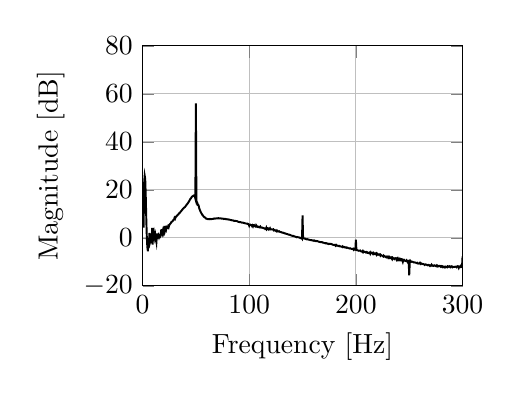
\begin{tikzpicture}

\begin{axis}[%
width=1.6in,
height=1.2in,
at={(0.758in,0.481in)},
scale only axis,
xmin=0,
xmax=300,
xmajorgrids,
ymin=-20,
ymax=80,
ymajorgrids,
ylabel={Magnitude [dB]},
xlabel={Frequency [Hz]},
axis background/.style={fill=white}
]
\addplot [color=black,solid,line width=0.7pt,forget plot]
  table[row sep=crcr]{%
0	13.3498984574393\\
0.500005208387587	17.9221189615137\\
1.00001041677517	4.25590051034798\\
1.50001562516276	22.938989504529\\
2.00002083355035	25.9318996116464\\
2.50002604193794	24.6481930941772\\
3.00003125032552	17.5970718132702\\
3.50003645871311	8.04625755442204\\
4.0000416671007	0.196303374004492\\
4.50004687548829	-3.88625171020054\\
5.00005208387587	-5.64060007042694\\
5.50005729226346	-0.643838837930736\\
6.00006250065105	-2.23120469485061\\
6.50006770903864	2.05806151850856\\
7.00007291742622	-1.85706045298493\\
7.50007812581381	-0.957577740819722\\
8.0000833342014	0.772408084428054\\
8.50008854258899	-2.30452707751395\\
9.00009375097657	4.14896908384729\\
9.50009895936416	-2.80695642050364\\
10.0001041677517	4.13359699892722\\
10.5001093761393	-0.832630499063016\\
11.0001145845269	1.38285705860543\\
11.5001197929145	-0.0574677899644654\\
12.0001250013021	1.11316449788151\\
12.5001302096897	-0.460259507550136\\
13.0001354180773	-1.76730880780609\\
13.5001406264649	1.40380141060239\\
14.0001458348524	1.44379543388979\\
14.50015104324	0.663546685582418\\
15.0001562516276	1.13176812732221\\
15.5001614600152	0.230312984358394\\
16.0001666684028	0.843012615829891\\
16.5001718767904	0.584314516864825\\
17.000177085178	1.21118427027218\\
17.5001822935656	3.17904214397736\\
18.0001875019531	3.25116868717505\\
18.5001927103407	2.003371747104\\
19.0001979187283	2.93711167822279\\
19.5002031271159	1.84468830460298\\
20.0002083355035	2.54832783065866\\
20.5002135438911	4.96826803715997\\
21.0002187522787	2.81820519545153\\
21.5002239606663	3.61534761149261\\
22.0002291690538	3.23820189364636\\
22.5002343774414	4.52905497541693\\
23.000239585829	4.33668876138591\\
23.5002447942166	4.18510922170639\\
24.0002500026042	4.84137699290434\\
24.5002552109918	4.43368023306746\\
25.0002604193794	5.32557470890088\\
25.500265627767	5.57289942217348\\
26.0002708361545	5.87210537647827\\
26.5002760445421	6.12270274644563\\
27.0002812529297	6.58765116605493\\
27.5002864613173	6.69639521250795\\
28.0002916697049	6.84854355755227\\
28.5002968780925	7.16342035912357\\
29.0003020864801	7.46869196866851\\
29.5003072948677	7.61112663086872\\
30.0003125032552	8.29470124024468\\
30.5003177116428	7.94404584883353\\
31.0003229200304	8.491879903215\\
31.500328128418	8.91572932622603\\
32.0003333368056	8.9998777884699\\
32.5003385451932	9.31105968534648\\
33.0003437535808	9.60300421227314\\
33.5003489619684	9.68075693300371\\
34.0003541703559	10.0878391317938\\
34.5003593787435	10.3360392804069\\
35.0003645871311	10.4477972189118\\
35.5003697955187	10.7639088273513\\
36.0003750039063	11.0124134238584\\
36.5003802122939	11.3035127148955\\
37.0003854206815	11.5555694096954\\
37.5003906290691	11.8678134432549\\
38.0003958374566	12.1291276158213\\
38.5004010458442	12.2925250646416\\
39.0004062542318	12.6014918745552\\
39.5004114626194	12.7242000652252\\
40.000416671007	12.9728138724306\\
40.5004218793946	13.2838684246326\\
41.0004270877822	13.5698869404533\\
41.5004322961697	13.9181299575647\\
42.0004375045573	14.1547711123594\\
42.5004427129449	14.4495981215517\\
43.0004479213325	14.8093397969334\\
43.5004531297201	15.1439719008231\\
44.0004583381077	15.5275560342276\\
44.5004635464953	15.9329455227933\\
45.0004687548829	16.3524198028163\\
45.5004739632705	16.5367478890092\\
46.000479171658	16.9663823438339\\
46.5004843800456	17.2090435298153\\
47.0004895884332	17.3424122307335\\
47.5004947968208	17.5147587639805\\
48.0005000052084	17.6144482383537\\
48.500505213596	17.4015428266318\\
49.0005104219836	17.1888703536532\\
49.5005156303711	16.3664676080797\\
50.0005208387587	56.0409772374937\\
50.5005260471463	15.5124953926494\\
51.0005312555339	14.8109911185613\\
51.5005364639215	14.3450061794357\\
52.0005416723091	13.6518286859175\\
52.5005468806967	13.5887502280519\\
53.0005520890843	12.5165172138655\\
53.5005572974719	11.8782792661584\\
54.0005625058594	11.2915875258998\\
54.500567714247	10.7770173294559\\
55.0005729226346	10.3661209547053\\
55.5005781310222	10.0202953829727\\
56.0005833394098	9.5383363162497\\
56.5005885477974	9.36987490895485\\
57.000593756185	9.04777978228318\\
57.5005989645725	8.74821526445267\\
58.0006041729601	8.6200144763045\\
58.5006093813477	8.49033978530965\\
59.0006145897353	8.23074809654405\\
59.5006197981229	8.0052272955166\\
60.0006250065105	8.00888612766212\\
60.5006302148981	7.86347337679698\\
61.0006354232857	7.80944741033046\\
61.5006406316732	7.79190908681665\\
62.0006458400608	7.78694364326875\\
62.5006510484484	7.84098415742542\\
63.000656256836	7.73869312515406\\
63.5006614652236	7.78633371693933\\
64.0006666736112	7.85160131889607\\
64.5006718819988	7.80053990039396\\
65.0006770903864	7.82476264306635\\
65.500682298774	7.857478605172\\
66.0006875071615	7.85335127982284\\
66.5006927155491	7.97507640891581\\
67.0006979239367	7.96651615326773\\
67.5007031323243	8.04954497394021\\
68.0007083407119	7.97108383993575\\
68.5007135490995	8.03974301987562\\
69.0007187574871	8.13865685433252\\
69.5007239658746	8.07228364335631\\
70.0007291742622	8.13222639222947\\
70.5007343826498	8.13482737134792\\
71.0007395910374	8.21656827392092\\
71.500744799425	8.06130850634079\\
72.0007500078126	8.10175388158663\\
72.5007552162002	8.11963695053116\\
73.0007604245878	8.10963060618245\\
73.5007656329753	8.0922485533706\\
74.0007708413629	8.00486082418392\\
74.5007760497505	7.96410475276938\\
75.0007812581381	8.01990762862287\\
75.5007864665257	7.98792734622022\\
76.0007916749133	7.84843267917602\\
76.5007968833009	7.90437956164312\\
77.0008020916885	7.85436360510377\\
77.500807300076	7.90426028077828\\
78.0008125084636	7.75543256735648\\
78.5008177168512	7.77941966740542\\
79.0008229252388	7.7070792257366\\
79.5008281336264	7.65078476048389\\
80.000833342014	7.72541059384636\\
80.5008385504016	7.64806241793264\\
81.0008437587892	7.54830434297173\\
81.5008489671767	7.56955410361516\\
82.0008541755643	7.51391905025352\\
82.5008593839519	7.43079011123957\\
83.0008645923395	7.38347332943811\\
83.5008698007271	7.33967178498138\\
84.0008750091147	7.23154947981463\\
84.5008802175023	7.27984195323175\\
85.0008854258898	7.23128488820534\\
85.5008906342774	7.14923274274593\\
86.000895842665	7.02687825672154\\
86.5009010510526	7.09136581295324\\
87.0009062594402	7.04363776246925\\
87.5009114678278	7.01737964610498\\
88.0009166762154	7.00017337900342\\
88.500921884603	6.93974108680073\\
89.0009270929906	6.85287432805122\\
89.5009323013781	6.70138797335543\\
90.0009375097657	6.64687467591347\\
90.5009427181533	6.61232802658376\\
91.0009479265409	6.50157827069079\\
91.5009531349285	6.54191126928564\\
92.0009583433161	6.51851320299016\\
92.5009635517037	6.43615604416402\\
93.0009687600913	6.32166644034989\\
93.5009739684788	6.3801972911158\\
94.0009791768664	6.33555078093851\\
94.500984385254	6.25882927654109\\
95.0009895936416	6.1943397521057\\
95.5009948020292	6.15710629196569\\
96.0010000104168	6.08452313102717\\
96.5010052188044	5.9671969671655\\
97.0010104271919	5.97475217154149\\
97.5010156355795	5.96033781224287\\
98.0010208439671	5.83984795889729\\
98.5010260523547	5.88658849664428\\
99.0010312607423	5.76933177055608\\
99.5010364691299	5.56161690095876\\
100.001041677517	5.0078930232793\\
100.501046885905	5.49938633372983\\
101.001052094293	5.50755201104647\\
101.50105730268	5.32770519667673\\
102.001062511068	5.31987748328721\\
102.501067719455	4.9556227724708\\
103.001072927843	5.21835144016822\\
103.501078136231	4.75481149643534\\
104.001083344618	5.29747019967069\\
104.501088553006	5.34033584603984\\
105.001093761393	4.91644601978386\\
105.501098969781	4.77842189519537\\
106.001104178169	4.67136309882387\\
106.501109386556	5.26395123825884\\
107.001114594944	4.95469054313204\\
107.501119803331	4.65047835785815\\
108.001125011719	4.49980659462546\\
108.501130220106	4.45532062204855\\
109.001135428494	4.61480695833538\\
109.501140636882	4.38035865512731\\
110.001145845269	4.30484238954891\\
110.501151053657	4.64534997719308\\
111.001156262044	4.32009808843429\\
111.501161470432	4.2708339794826\\
112.00116667882	4.21965927934431\\
112.501171887207	4.24312734147366\\
113.001177095595	4.09166165212412\\
113.501182303982	4.04853862021305\\
114.00118751237	3.96890526342923\\
114.501192720758	3.908745958396\\
115.001197929145	3.64784949280756\\
115.501203137533	3.66235287415194\\
116.00120834592	4.18733752255416\\
116.501213554308	3.46850380194794\\
117.001218762695	3.69145024625499\\
117.501223971083	3.99175811404185\\
118.001229179471	3.96548503201363\\
118.501234387858	3.4840342008568\\
119.001239596246	3.6911485604272\\
119.501244804633	3.98826094262537\\
120.001250013021	3.51640114929115\\
120.501255221409	3.57261555580399\\
121.001260429796	3.51594582524362\\
121.501265638184	3.46319789444494\\
122.001270846571	3.45769339352851\\
122.501276054959	3.56177683725952\\
123.001281263347	3.03558793919643\\
123.501286471734	3.04589826799027\\
124.001291680122	3.21419615778702\\
124.501296888509	3.00660147865749\\
125.001302096897	2.86551971191449\\
125.501307305284	2.71077263515976\\
126.001312513672	3.06518662622245\\
126.50131772206	2.83684811454294\\
127.001322930447	2.60454336297939\\
127.501328138835	2.66439708356649\\
128.001333347222	2.75767296231653\\
128.50133855561	2.57481385254642\\
129.001343763998	2.42303176747926\\
129.501348972385	2.39664151136911\\
130.001354180773	2.36277131164005\\
130.50135938916	2.24793908394457\\
131.001364597548	2.16196717794009\\
131.501369805935	2.17932364466847\\
132.001375014323	2.01299167110504\\
132.501380222711	2.02014054583756\\
133.001385431098	1.88607402298835\\
133.501390639486	1.88368415167709\\
134.001395847873	1.78593430711825\\
134.501401056261	1.69216517084848\\
135.001406264649	1.62023035169422\\
135.501411473036	1.59484274592765\\
136.001416681424	1.52299351097127\\
136.501421889811	1.37536671636645\\
137.001427098199	1.33511055007872\\
137.501432306587	1.32344434777133\\
138.001437514974	1.25184928963781\\
138.501442723362	1.15007616950875\\
139.001447931749	1.0686915433005\\
139.501453140137	0.944090636432949\\
140.001458348524	0.871198639528432\\
140.501463556912	0.84293918991249\\
141.0014687653	0.76566580762075\\
141.501473973687	0.769309500823615\\
142.001479182075	0.649389369565021\\
142.501484390462	0.570327209451932\\
143.00148959885	0.515053710290056\\
143.501494807238	0.421166201154447\\
144.001500015625	0.348988119613332\\
144.501505224013	0.243371629254346\\
145.0015104324	0.335435396435283\\
145.501515640788	0.28038396073284\\
146.001520849176	0.226731527785474\\
146.501526057563	0.213132431831498\\
147.001531265951	0.051033232848171\\
147.501536474338	0.0661572652002537\\
148.001541682726	-0.129388512331934\\
148.501546891113	-0.167548253269282\\
149.001552099501	-0.049555029917951\\
149.501557307889	-0.34095104617568\\
150.001562516276	9.36318983453923\\
150.501567724664	-0.0110981879202958\\
151.001572933051	-0.151906051737656\\
151.501578141439	-0.320459946190696\\
152.001583349827	-0.365524298204517\\
152.501588558214	-0.3496457378955\\
153.001593766602	-0.482896294776936\\
153.501598974989	-0.562509794637779\\
154.001604183377	-0.634561052178894\\
154.501609391765	-0.565111722283888\\
155.001614600152	-0.658685564675226\\
155.50161980854	-0.747612254196178\\
156.001625016927	-0.790932876179348\\
156.501630225315	-0.800396134883094\\
157.001635433702	-0.923470032775575\\
157.50164064209	-0.914700349759252\\
158.001645850478	-1.00430772150444\\
158.501651058865	-0.960281903058526\\
159.001656267253	-1.09400302543301\\
159.50166147564	-1.1318161852454\\
160.001666684028	-1.09452826792187\\
160.501671892416	-1.19714740357714\\
161.001677100803	-1.08959542910015\\
161.501682309191	-1.26378610492152\\
162.001687517578	-1.36050029318097\\
162.501692725966	-1.28313340607271\\
163.001697934353	-1.34515647905527\\
163.501703142741	-1.41814739916492\\
164.001708351129	-1.37780242278623\\
164.501713559516	-1.50599507951443\\
165.001718767904	-1.57058388508356\\
165.501723976291	-1.65564991224703\\
166.001729184679	-1.69028604896342\\
166.501734393067	-1.76992232469053\\
167.001739601454	-1.80059128034962\\
167.501744809842	-1.76502679687766\\
168.001750018229	-1.7737363927073\\
168.501755226617	-1.88053549642059\\
169.001760435005	-2.00170734442624\\
169.501765643392	-1.9681845306337\\
170.00177085178	-2.08020347241161\\
170.501776060167	-2.17056906215902\\
171.001781268555	-2.18943423135252\\
171.501786476942	-2.21777872830016\\
172.00179168533	-2.35071383476591\\
172.501796893718	-2.24592037635726\\
173.001802102105	-2.3815797635825\\
173.501807310493	-2.41928188633937\\
174.00181251888	-2.54077105178378\\
174.501817727268	-2.62758348965572\\
175.001822935656	-2.47803404227973\\
175.501828144043	-2.55109694258445\\
176.001833352431	-2.58224942206581\\
176.501838560818	-2.53845532864388\\
177.001843769206	-2.57167346701566\\
177.501848977594	-2.6684717409905\\
178.001854185981	-2.88361415604665\\
178.501859394369	-2.91001121773624\\
179.001864602756	-2.95196516996208\\
179.501869811144	-3.0032751857869\\
180.001875019531	-2.929760471383\\
180.501880227919	-2.95287778462897\\
181.001885436307	-3.28210227073936\\
181.501890644694	-2.98380435042335\\
182.001895853082	-3.25784036473448\\
182.501901061469	-3.23776569779945\\
183.001906269857	-3.28360776500442\\
183.501911478245	-3.44656382156058\\
184.001916686632	-3.34554033541255\\
184.50192189502	-3.37361078132937\\
185.001927103407	-3.59940203137162\\
185.501932311795	-3.57092584559476\\
186.001937520183	-3.6226258439284\\
186.50194272857	-3.67829207017227\\
187.001947936958	-3.78059827987441\\
187.501953145345	-3.56475589368083\\
188.001958353733	-3.87691382120684\\
188.50196356212	-3.74830629967984\\
189.001968770508	-3.79444797522425\\
189.501973978896	-3.9802934038959\\
190.001979187283	-3.92028055838075\\
190.501984395671	-3.93298020120907\\
191.001989604058	-4.15746230287297\\
191.501994812446	-4.0191065635412\\
192.002000020834	-4.07255706190452\\
192.502005229221	-4.19166454846468\\
193.002010437609	-4.33513621721578\\
193.502015645996	-4.35082936901048\\
194.002020854384	-4.44193661471982\\
194.502026062771	-4.34040002446987\\
195.002031271159	-4.4850186138154\\
195.502036479547	-4.56034207885079\\
196.002041687934	-4.62851562254434\\
196.502046896322	-4.64422778352349\\
197.002052104709	-4.69340710895796\\
197.502057313097	-4.5576866625981\\
198.002062521485	-5.00715798482153\\
198.502067729872	-4.7779301825145\\
199.00207293826	-4.9025737703485\\
199.502078146647	-4.76920104205395\\
200.002083355035	-0.732225312325501\\
200.502088563423	-5.10492413523921\\
201.00209377181	-5.13976355630009\\
201.502098980198	-5.16810476019073\\
202.002104188585	-5.2937749803118\\
202.502109396973	-5.40153254040561\\
203.00211460536	-5.3465721305921\\
203.502119813748	-5.35876494814802\\
204.002125022136	-5.28498172819732\\
204.502130230523	-5.57062065175539\\
205.002135438911	-5.63540033123444\\
205.502140647298	-5.61708431538262\\
206.002145855686	-5.84832135330656\\
206.502151064074	-5.50482452695493\\
207.002156272461	-5.94936172335676\\
207.502161480849	-5.69399167096268\\
208.002166689236	-5.81401678900682\\
208.502171897624	-5.87435511650136\\
209.002177106012	-5.93685909707209\\
209.502182314399	-6.12546656720757\\
210.002187522787	-5.89037953929228\\
210.502192731174	-5.99526227021411\\
211.002197939562	-6.29003781429605\\
211.502203147949	-6.2414208873036\\
212.002208356337	-6.35287866975773\\
212.502213564725	-6.10525824974121\\
213.002218773112	-6.07952672301533\\
213.5022239815	-6.6128651355473\\
214.002229189887	-6.09370222925188\\
214.502234398275	-6.44845293242131\\
215.002239606663	-6.42636028589602\\
215.50224481505	-6.30527295532054\\
216.002250023438	-6.6652848234477\\
216.502255231825	-6.33710694138786\\
217.002260440213	-6.71333493699489\\
217.502265648601	-6.50383821241292\\
218.002270856988	-6.50487580319508\\
218.502276065376	-6.74696023681384\\
219.002281273763	-6.4948609302611\\
219.502286482151	-7.01038112151788\\
220.002291690538	-6.58717021927338\\
220.502296898926	-6.76764826779533\\
221.002302107314	-7.06288099918086\\
221.502307315701	-6.9973853655233\\
222.002312524089	-6.9386935470809\\
222.502317732476	-6.86000983370461\\
223.002322940864	-7.42515134957046\\
223.502328149252	-7.15442565058114\\
224.002333357639	-7.33471243013932\\
224.502338566027	-7.45810676197023\\
225.002343774414	-7.52149767580215\\
225.502348982802	-7.75232644010804\\
226.002354191189	-7.41572961478512\\
226.502359399577	-7.7891059558185\\
227.002364607965	-7.65874936629919\\
227.502369816352	-7.78683529758072\\
228.00237502474	-8.01270982633131\\
228.502380233127	-7.87362446059049\\
229.002385441515	-8.18259402599404\\
229.502390649903	-8.12638717602762\\
230.00239585829	-7.88087361572085\\
230.502401066678	-8.42188235281187\\
231.002406275065	-8.2484467782471\\
231.502411483453	-8.01020331732159\\
232.002416691841	-8.43818562991292\\
232.502421900228	-8.28381940933447\\
233.002427108616	-8.14018623123818\\
233.502432317003	-8.54128622130997\\
234.002437525391	-8.90883648012983\\
234.502442733778	-8.25826562417983\\
235.002447942166	-8.43989227402533\\
235.502453150554	-8.63000450684797\\
236.002458358941	-8.82922940078964\\
236.502463567329	-8.507900449133\\
237.002468775716	-8.46751785384805\\
237.502473984104	-8.55578828521039\\
238.002479192492	-9.00265338806746\\
238.502484400879	-8.46501615526865\\
239.002489609267	-8.36069074658804\\
239.502494817654	-9.39814759398329\\
240.002500026042	-9.36596643017019\\
240.50250523443	-8.6657430596525\\
241.002510442817	-8.61446041449466\\
241.502515651205	-9.41733878214241\\
242.002520859592	-9.39336572645479\\
242.50252606798	-8.82840914484748\\
243.002531276367	-8.82862729530092\\
243.502536484755	-9.2700781216775\\
244.002541693143	-9.97201997320965\\
244.50254690153	-9.13570011982657\\
245.002552109918	-9.11456969730209\\
245.502557318305	-9.43510698473645\\
246.002562526693	-9.57516878924688\\
246.502567735081	-9.67747041367868\\
247.002572943468	-9.56001913074662\\
247.502578151856	-9.33872998808765\\
248.002583360243	-9.77652844901527\\
248.502588568631	-10.1283415096371\\
249.002593777019	-9.67708451647453\\
249.502598985406	-9.59419669607718\\
250.002604193794	-15.6661140182521\\
250.502609402181	-10.3060770522045\\
251.002614610569	-9.58496405906905\\
251.502619818956	-9.86151994342413\\
252.002625027344	-10.0191680629628\\
252.502630235732	-9.93633331770335\\
253.002635444119	-9.96822712973407\\
253.502640652507	-10.0577065939067\\
254.002645860894	-10.2165376212235\\
254.502651069282	-10.2154644851229\\
255.00265627767	-10.221105922395\\
255.502661486057	-10.3086453865788\\
256.002666694445	-10.3688151406314\\
256.502671902832	-10.3922344447329\\
257.00267711122	-10.5275290970542\\
257.502682319608	-10.3992250193728\\
258.002687527995	-10.6955011165062\\
258.502692736383	-10.729397945327\\
259.00269794477	-10.6954974734613\\
259.502703153158	-10.6268490805053\\
260.002708361545	-10.3947031618983\\
260.502713569933	-10.8331599486818\\
261.002718778321	-10.6120652155174\\
261.502723986708	-10.7564373145285\\
262.002729195096	-10.9240903386235\\
262.502734403483	-10.8407436105825\\
263.002739611871	-10.9402431977602\\
263.502744820259	-10.9622465055625\\
264.002750028646	-11.0945855706158\\
264.502755237034	-11.3071331133363\\
265.002760445421	-11.1027636088589\\
265.502765653809	-11.0825036200717\\
266.002770862196	-11.2021390563778\\
266.502776070584	-11.2309590735245\\
267.002781278972	-11.4177807570556\\
267.502786487359	-11.4759902323232\\
268.002791695747	-11.2977593193794\\
268.502796904134	-11.3104186001334\\
269.002802112522	-11.4501557485672\\
269.50280732091	-11.7328663996477\\
270.002812529297	-11.5332632319935\\
270.502817737685	-11.596706980566\\
271.002822946072	-11.1898180487473\\
271.50282815446	-11.514177864251\\
272.002833362848	-11.6385138385402\\
272.502838571235	-11.7437402193808\\
273.002843779623	-11.686788825334\\
273.50284898801	-11.4505128258335\\
274.002854196398	-11.5083092473621\\
274.502859404785	-11.6541041862402\\
275.002864613173	-11.8317525385542\\
275.502869821561	-11.8714026930523\\
276.002875029948	-11.4442413015966\\
276.502880238336	-11.6327512539767\\
277.002885446723	-11.9174515756042\\
277.502890655111	-11.7277032610067\\
278.002895863499	-11.7694777319058\\
278.502901071886	-11.6945063945898\\
279.002906280274	-11.872108919534\\
279.502911488661	-12.0541915989548\\
280.002916697049	-11.7510612184913\\
280.502921905436	-11.8337404526253\\
281.002927113824	-12.1483170165874\\
281.502932322212	-11.8748570701095\\
282.002937530599	-12.0287690794133\\
282.502942738987	-12.2383477465803\\
283.002947947374	-12.103111118201\\
283.502953155762	-12.3183537523831\\
284.00295836415	-11.9881356129484\\
284.502963572537	-12.0517757843538\\
285.002968780925	-12.0514101590312\\
285.502973989312	-12.2586774967436\\
286.0029791977	-11.9205293911061\\
286.502984406088	-12.1212130492136\\
287.002989614475	-12.0193397281741\\
287.502994822863	-11.8261677082659\\
288.00300003125	-11.968879886705\\
288.503005239638	-12.2655734104179\\
289.003010448026	-12.0394579132991\\
289.503015656413	-11.8365944920951\\
290.003020864801	-11.8699313984269\\
290.503026073188	-12.2562097148267\\
291.003031281576	-12.1010669670127\\
291.503036489963	-12.1603519018529\\
292.003041698351	-12.1689208642218\\
292.503046906739	-12.0567398071156\\
293.003052115126	-12.0978775588781\\
293.503057323514	-12.0172311323759\\
294.003062531901	-11.9819522375654\\
294.503067740289	-12.2353149783524\\
295.003072948677	-11.9084287979772\\
295.503078157064	-11.7997175023605\\
296.003083365452	-11.8985120371164\\
296.503088573839	-12.5177121419284\\
297.003093782227	-12.0352551323083\\
297.503098990614	-12.114947225917\\
298.003104199002	-11.7995500455465\\
298.50310940739	-12.2006224223399\\
299.003114615777	-12.1629825136024\\
299.503119824165	-12.0195144203994\\
300.003125032552	-7.7683549740539\\
};
\end{axis}
\end{tikzpicture}%
    \caption{Measurement 1 (mic).}
    \label{fig:FFT_mic1_50Hz}
\end{subfigure}
\begin{subfigure}[t]{0.28\textwidth}
    \tikzsetnextfilename{FFT_mic6_50Hz}
    % This file was created by matlab2tikz.
%
%The latest updates can be retrieved from
%  http://www.mathworks.com/matlabcentral/fileexchange/22022-matlab2tikz-matlab2tikz
%where you can also make suggestions and rate matlab2tikz.
%
\definecolor{mycolor1}{rgb}{0.00000,0.44700,0.74100}%
%
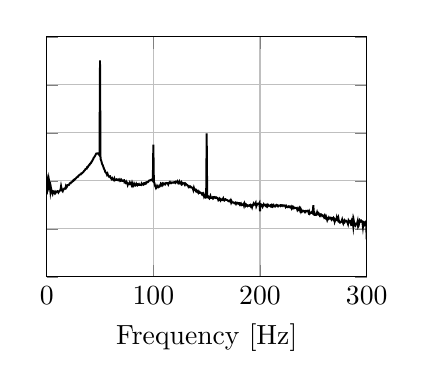
\begin{tikzpicture}

\begin{axis}[%
width=1.6in,
height=1.2in,
at={(0.758in,0.481in)},
scale only axis,
xmin=0,
xmax=300,
xmajorgrids,
ymin=-20,
ymax=80,
ymajorgrids,
yticklabels={\empty},
xlabel={Frequency [Hz]},
axis background/.style={fill=white}
]
\addplot [color=black,solid,line width=0.7pt,forget plot]
  table[row sep=crcr]{%
0	14.3787069686561\\
0.500005208387587	16.0141699979174\\
1.00001041677517	19.613120823683\\
1.50001562516276	18.4271203508735\\
2.00002083355035	20.7177813192485\\
2.50002604193794	19.4630022319103\\
3.00003125032552	17.5401902133973\\
3.50003645871311	15.4713245210484\\
4.0000416671007	17.1113624161801\\
4.50004687548829	15.8892613900536\\
5.00005208387587	15.2525366222125\\
5.50005729226346	14.6513612537425\\
6.00006250065105	15.70906874288\\
6.50006770903864	15.5943341209826\\
7.00007291742622	15.1337181217248\\
7.50007812581381	14.8366986460195\\
8.0000833342014	15.444387060191\\
8.50008854258899	15.0698778020914\\
9.00009375097657	15.4122421902295\\
9.50009895936416	15.5400140782681\\
10.0001041677517	15.743541354351\\
10.5001093761393	15.6751648012737\\
11.0001145845269	15.1795608321697\\
11.5001197929145	15.5488213073488\\
12.0001250013021	15.8287918650328\\
12.5001302096897	16.0192835722286\\
13.0001354180773	16.4231150525721\\
13.5001406264649	17.8054729251336\\
14.0001458348524	16.7543122933631\\
14.50015104324	15.9478889443683\\
15.0001562516276	15.664953252965\\
15.5001614600152	16.3563063608446\\
16.0001666684028	16.4457118535299\\
16.5001718767904	16.824344042179\\
17.000177085178	16.8865160941427\\
17.5001822935656	16.7920449207556\\
18.0001875019531	17.7414798194926\\
18.5001927103407	17.2363046130962\\
19.0001979187283	17.5383000343804\\
19.5002031271159	18.2195490810073\\
20.0002083355035	18.206819415899\\
20.5002135438911	18.2836650594635\\
21.0002187522787	18.362313373058\\
21.5002239606663	18.9153773676596\\
22.0002291690538	19.0853899059052\\
22.5002343774414	19.0444206398509\\
23.000239585829	19.4271599886477\\
23.5002447942166	19.4642231041327\\
24.0002500026042	19.7227968349871\\
24.5002552109918	20.0716997314211\\
25.0002604193794	20.0034250143654\\
25.500265627767	20.4494893388246\\
26.0002708361545	20.3730517593147\\
26.5002760445421	20.7521883164259\\
27.0002812529297	20.8578108715422\\
27.5002864613173	21.1148503080664\\
28.0002916697049	21.4190181777412\\
28.5002968780925	21.5384578941962\\
29.0003020864801	21.7645052525534\\
29.5003072948677	21.7769423514397\\
30.0003125032552	22.2279625244544\\
30.5003177116428	22.3923841630576\\
31.0003229200304	22.5989368890602\\
31.500328128418	22.7345616786155\\
32.0003333368056	22.7238784260358\\
32.5003385451932	23.1211113331878\\
33.0003437535808	23.1329725932246\\
33.5003489619684	23.3089666757163\\
34.0003541703559	23.5299098895839\\
34.5003593787435	23.7496319600308\\
35.0003645871311	24.0830630847604\\
35.5003697955187	24.3529284048889\\
36.0003750039063	24.5866424178925\\
36.5003802122939	24.9807448293813\\
37.0003854206815	25.0365889905334\\
37.5003906290691	25.0896550994042\\
38.0003958374566	25.7489135865616\\
38.5004010458442	25.7131076387641\\
39.0004062542318	26.1714251265537\\
39.5004114626194	26.4935363408904\\
40.000416671007	26.5496435890566\\
40.5004218793946	27.1295532174654\\
41.0004270877822	27.1867615318763\\
41.5004322961697	27.4668697356012\\
42.0004375045573	27.9406945143417\\
42.5004427129449	28.1060989230547\\
43.0004479213325	28.6707370859533\\
43.5004531297201	28.9414514517466\\
44.0004583381077	29.5658504095071\\
44.5004635464953	29.7760559942555\\
45.0004687548829	30.180209044394\\
45.5004739632705	30.5520880259132\\
46.000479171658	31.0014432692874\\
46.5004843800456	31.3949254287456\\
47.0004895884332	31.3862479039584\\
47.5004947968208	31.5111185388562\\
48.0005000052084	31.4883141385303\\
48.500505213596	31.2487756602325\\
49.0005104219836	31.009973972683\\
49.5005156303711	30.6725350516691\\
50.0005208387587	70.2261397476465\\
50.5005260471463	29.1062946486401\\
51.0005312555339	28.6272577151846\\
51.5005364639215	27.8516914037039\\
52.0005416723091	27.0186838918862\\
52.5005468806967	26.6249941565777\\
53.0005520890843	25.9846166999852\\
53.5005572974719	25.3734625991752\\
54.0005625058594	24.8191195528423\\
54.500567714247	24.3655920776041\\
55.0005729226346	23.6696796919556\\
55.5005781310222	23.4381850562818\\
56.0005833394098	23.28151282977\\
56.5005885477974	22.6555076816432\\
57.000593756185	23.0478401208241\\
57.5005989645725	22.4123243357314\\
58.0006041729601	22.0696871023675\\
58.5006093813477	21.7379772228707\\
59.0006145897353	21.8257422668107\\
59.5006197981229	21.895603364297\\
60.0006250065105	21.2915385509514\\
60.5006302148981	20.9871248645616\\
61.0006354232857	20.6964001546946\\
61.5006406316732	21.0797212705527\\
62.0006458400608	20.6235387397028\\
62.5006510484484	20.5762572296028\\
63.000656256836	20.3156952942213\\
63.5006614652236	20.9716085578025\\
64.0006666736112	20.2972486029491\\
64.5006718819988	20.3303314669047\\
65.0006770903864	20.5178558193944\\
65.500682298774	20.6549397178899\\
66.0006875071615	20.3723127240889\\
66.5006927155491	20.3293018739823\\
67.0006979239367	20.5285755664758\\
67.5007031323243	20.2066887301099\\
68.0007083407119	20.1729397950315\\
68.5007135490995	20.5078170668202\\
69.0007187574871	19.9396934954476\\
69.5007239658746	20.0186852254833\\
70.0007291742622	20.4649624744856\\
70.5007343826498	20.1896890516153\\
71.0007395910374	19.9633044906706\\
71.500744799425	19.9518058568566\\
72.0007500078126	20.2525754596984\\
72.5007552162002	20.278244176711\\
73.0007604245878	19.3668204220907\\
73.5007656329753	19.4641545595959\\
74.0007708413629	19.2021714628398\\
74.5007760497505	19.6636910582927\\
75.0007812581381	19.1398467634607\\
75.5007864665257	19.198748211582\\
76.0007916749133	18.3535336704117\\
76.5007968833009	18.9326038485134\\
77.0008020916885	18.8511354460271\\
77.500807300076	18.7161361850394\\
78.0008125084636	19.327794242476\\
78.5008177168512	18.8699866170339\\
79.0008229252388	18.9502197917448\\
79.5008281336264	18.3591642417161\\
80.000833342014	19.142798284203\\
80.5008385504016	18.3219372991317\\
81.0008437587892	17.7539184920148\\
81.5008489671767	18.0192375677286\\
82.0008541755643	18.7436832331369\\
82.5008593839519	18.2022916016344\\
83.0008645923395	18.0345082561169\\
83.5008698007271	18.2215559063826\\
84.0008750091147	18.7748035742009\\
84.5008802175023	18.298204337777\\
85.0008854258898	18.1262503975437\\
85.5008906342774	18.547038939149\\
86.000895842665	18.4163766679326\\
86.5009010510526	18.6853333165965\\
87.0009062594402	18.3335573395092\\
87.5009114678278	18.3677771683436\\
88.0009166762154	18.2958582672654\\
88.500921884603	18.2766595398936\\
89.0009270929906	18.9044011962705\\
89.5009323013781	18.543013933189\\
90.0009375097657	18.6990063428429\\
90.5009427181533	18.4945345099084\\
91.0009479265409	18.8915025809163\\
91.5009531349285	18.7233530094893\\
92.0009583433161	19.1177657940699\\
92.5009635517037	19.2385065783708\\
93.0009687600913	18.8931075730293\\
93.5009739684788	19.1308635242308\\
94.0009791768664	19.5109676703476\\
94.500984385254	19.6037994522767\\
95.0009895936416	19.5365886515897\\
95.5009948020292	19.7775839154235\\
96.0010000104168	20.123594738295\\
96.5010052188044	20.1693734493345\\
97.0010104271919	20.2714043629629\\
97.5010156355795	20.2341617017122\\
98.0010208439671	20.462322978312\\
98.5010260523547	20.5830907288805\\
99.0010312607423	20.3057167110357\\
99.5010364691299	20.0196676680361\\
100.001041677517	35.1285554284599\\
100.501046885905	19.6939525908583\\
101.001052094293	19.1969807784565\\
101.50105730268	18.0379443834427\\
102.001062511068	17.658639723728\\
102.501067719455	16.9696075521659\\
103.001072927843	17.2907115861\\
103.501078136231	17.9114463159964\\
104.001083344618	17.4751767491161\\
104.501088553006	17.3089036401532\\
105.001093761393	17.4785351265463\\
105.501098969781	17.9336573848886\\
106.001104178169	17.7199576256119\\
106.501109386556	18.0320132837216\\
107.001114594944	18.8130128692172\\
107.501119803331	18.5258765810124\\
108.001125011719	18.170612373384\\
108.501130220106	18.7517639512313\\
109.001135428494	18.4081878927254\\
109.501140636882	18.8382126710047\\
110.001145845269	18.6321042410281\\
110.501151053657	18.8176079491365\\
111.001156262044	18.5751684096455\\
111.501161470432	19.0282215971618\\
112.00116667882	18.974042936103\\
112.501171887207	19.1036565357717\\
113.001177095595	18.9418403915033\\
113.501182303982	19.0407564885335\\
114.00118751237	18.5285619512025\\
114.501192720758	19.0597866695261\\
115.001197929145	19.2048697051785\\
115.501203137533	19.506445507034\\
116.00120834592	19.0799362360104\\
116.501213554308	19.0056210671374\\
117.001218762695	19.2253540531772\\
117.501223971083	19.3757957503611\\
118.001229179471	19.2729683889306\\
118.501234387858	19.2101447178433\\
119.001239596246	19.2408540534501\\
119.501244804633	19.5030696028966\\
120.001250013021	19.4852027460283\\
120.501255221409	19.2007984804316\\
121.001260429796	19.5829827353694\\
121.501265638184	19.3769754892548\\
122.001270846571	19.392094551272\\
122.501276054959	19.7867805829348\\
123.001281263347	19.2742663475589\\
123.501286471734	18.8926491732197\\
124.001291680122	18.9140986474589\\
124.501296888509	19.6380324132956\\
125.001302096897	19.0921350314069\\
125.501307305284	19.2467929459022\\
126.001312513672	18.8177392867492\\
126.50131772206	19.3100186677464\\
127.001322930447	18.6992587769854\\
127.501328138835	19.0311465696263\\
128.001333347222	18.9665806607898\\
128.50133855561	19.0548921778174\\
129.001343763998	18.7956665272184\\
129.501348972385	18.38469452462\\
130.001354180773	18.9626363677701\\
130.50135938916	18.7857939930555\\
131.001364597548	18.4500829397169\\
131.501369805935	18.389491216243\\
132.001375014323	18.1174750758828\\
132.501380222711	18.0204917240719\\
133.001385431098	17.4987715481726\\
133.501390639486	17.7285332598234\\
134.001395847873	17.4026570609586\\
134.501401056261	17.3225499220095\\
135.001406264649	17.6166858475698\\
135.501411473036	17.3823660871194\\
136.001416681424	17.2166125785682\\
136.501421889811	17.1454974567768\\
137.001427098199	16.909047899454\\
137.501432306587	16.1887326215668\\
138.001437514974	17.0818356268114\\
138.501442723362	16.3706711273369\\
139.001447931749	16.4798449879433\\
139.501453140137	16.0609356916829\\
140.001458348524	15.7080751557892\\
140.501463556912	16.0583392771387\\
141.0014687653	15.5986844433782\\
141.501473973687	15.3186034253901\\
142.001479182075	15.6337823120415\\
142.501484390462	15.0756437714783\\
143.00148959885	15.3974000548978\\
143.501494807238	15.0754708962634\\
144.001500015625	15.1948764066891\\
144.501505224013	15.0737593935467\\
145.0015104324	14.8056806464399\\
145.501515640788	14.4467870128926\\
146.001520849176	14.7077656333455\\
146.501526057563	14.2548888776454\\
147.001531265951	14.603256994296\\
147.501536474338	13.6283499589828\\
148.001541682726	14.1665689453911\\
148.501546891113	13.9632706885131\\
149.001552099501	13.1456480545144\\
149.501557307889	13.3010935410729\\
150.001562516276	39.7467177859958\\
150.501567724664	13.1548364887178\\
151.001572933051	13.1536996406762\\
151.501578141439	13.3763717094424\\
152.001583349827	12.9392185926486\\
152.501588558214	12.6904317601426\\
153.001593766602	13.2252408776693\\
153.501598974989	13.7574880522151\\
154.001604183377	12.912169225285\\
154.501609391765	12.8831453039692\\
155.001614600152	12.8899563661871\\
155.50161980854	13.101894053084\\
156.001625016927	12.6113969399886\\
156.501630225315	12.7830265805539\\
157.001635433702	13.2522551930834\\
157.50164064209	13.3039612913449\\
158.001645850478	12.9707635892905\\
158.501651058865	12.8823531410738\\
159.001656267253	13.1050572678079\\
159.50166147564	12.9249019897459\\
160.001666684028	12.9154233308549\\
160.501671892416	12.514853964355\\
161.001677100803	11.9194380293289\\
161.501682309191	12.1067994071318\\
162.001687517578	12.5982251615595\\
162.501692725966	12.2544100336272\\
163.001697934353	11.855779622119\\
163.501703142741	12.366979513511\\
164.001708351129	12.1733580052752\\
164.501713559516	12.0570989480632\\
165.001718767904	12.310630565632\\
165.501723976291	12.7224289222822\\
166.001729184679	11.9299000266241\\
166.501734393067	11.8342082283671\\
167.001739601454	12.3592653366825\\
167.501744809842	12.3990681354571\\
168.001750018229	12.1244934392457\\
168.501755226617	12.0798901048618\\
169.001760435005	12.0386622438912\\
169.501765643392	11.9405989014458\\
170.00177085178	11.7384913866055\\
170.501776060167	11.5161492693138\\
171.001781268555	11.4769850795243\\
171.501786476942	11.7301443581484\\
172.00179168533	11.4753252529895\\
172.501796893718	11.8928407722351\\
173.001802102105	10.9371379338641\\
173.501807310493	11.4376582916204\\
174.00181251888	11.0004473548423\\
174.501817727268	11.1016328341189\\
175.001822935656	11.1012688560836\\
175.501828144043	10.9868445319201\\
176.001833352431	10.6230737859439\\
176.501838560818	10.5858535859822\\
177.001843769206	10.8564104752994\\
177.501848977594	10.4211718190456\\
178.001854185981	10.8693301533283\\
178.501859394369	10.9373273372753\\
179.001864602756	10.8608030865082\\
179.501869811144	10.5256054344354\\
180.001875019531	10.7135299474972\\
180.501880227919	10.7218869679356\\
181.001885436307	10.1985330964982\\
181.501890644694	10.4881120136367\\
182.001895853082	10.6799201184784\\
182.501901061469	9.83720288658834\\
183.001906269857	9.88434980831423\\
183.501911478245	9.96136744580745\\
184.001916686632	10.237730816888\\
184.50192189502	10.4427790969256\\
185.001927103407	9.6973288817751\\
185.501932311795	10.65078684121\\
186.001937520183	10.1562241394985\\
186.50194272857	9.66689432594176\\
187.001947936958	10.0737932598471\\
187.501953145345	9.71817240421625\\
188.001958353733	9.83903916160094\\
188.50196356212	9.49767427308346\\
189.001968770508	9.72571051097552\\
189.501973978896	9.66615488497856\\
190.001979187283	9.85391590221536\\
190.501984395671	9.65011480860736\\
191.001989604058	9.8864065206398\\
191.501994812446	9.32552126724569\\
192.002000020834	9.57576252589422\\
192.502005229221	9.02835305300197\\
193.002010437609	9.98107687613249\\
193.502015645996	9.91000554316606\\
194.002020854384	10.5697133527414\\
194.502026062771	10.1704106519332\\
195.002031271159	10.4488500159093\\
195.502036479547	10.3236166754039\\
196.002041687934	10.808635658054\\
196.502046896322	9.44958056004687\\
197.002052104709	10.0081206184377\\
197.502057313097	10.2859930885577\\
198.002062521485	10.5525189405576\\
198.502067729872	10.5467727468703\\
199.00207293826	10.3016775746623\\
199.502078146647	10.7376204517022\\
200.002083355035	7.34382119590547\\
200.502088563423	10.3089347575633\\
201.00209377181	10.2588084665788\\
201.502098980198	10.0798742665627\\
202.002104188585	9.90650330928209\\
202.502109396973	9.24824004227409\\
203.00211460536	9.70541679438375\\
203.502119813748	10.2514186732859\\
204.002125022136	9.8492235628165\\
204.502130230523	9.89059757142506\\
205.002135438911	9.67350296888489\\
205.502140647298	9.95415652804241\\
206.002145855686	9.44425598288117\\
206.502151064074	9.73868172415335\\
207.002156272461	9.43476645641574\\
207.502161480849	10.0474443602345\\
208.002166689236	9.76195598678964\\
208.502171897624	9.65090811654353\\
209.002177106012	9.69673981885013\\
209.502182314399	9.50737999343711\\
210.002187522787	9.94490961278475\\
210.502192731174	10.0494357945482\\
211.002197939562	9.22466581389671\\
211.502203147949	9.156937973748\\
212.002208356337	10.035851709272\\
212.502213564725	10.112368574396\\
213.002218773112	9.44087250275833\\
213.5022239815	9.48079197149369\\
214.002229189887	9.33751642426721\\
214.502234398275	9.71970358962569\\
215.002239606663	9.87327727262096\\
215.50224481505	10.0116389891583\\
216.002250023438	9.64603428058818\\
216.502255231825	9.75883194394473\\
217.002260440213	9.3826139855166\\
217.502265648601	9.56361513494796\\
218.002270856988	9.71516382871787\\
218.502276065376	9.75730249414289\\
219.002281273763	9.85458371491143\\
219.502286482151	9.4976961454422\\
220.002291690538	9.62948196996635\\
220.502296898926	9.88450632515054\\
221.002302107314	9.85469990639748\\
221.502307315701	9.56476149691608\\
222.002312524089	9.82479841437834\\
222.502317732476	9.83573198030159\\
223.002322940864	9.68454377993916\\
223.502328149252	9.60697323324241\\
224.002333357639	9.16275104271966\\
224.502338566027	9.63125380572192\\
225.002343774414	9.2899835165178\\
225.502348982802	9.10955136295832\\
226.002354191189	9.04237811872927\\
226.502359399577	9.32166892248832\\
227.002364607965	9.42195923435102\\
227.502369816352	9.18483265242853\\
228.00237502474	9.02791775794365\\
228.502380233127	9.33419259060567\\
229.002385441515	9.21934605729051\\
229.502390649903	8.67202822193329\\
230.00239585829	9.39510188193651\\
230.502401066678	9.18951236553931\\
231.002406275065	8.6945887323822\\
231.502411483453	9.09708831821066\\
232.002416691841	8.87944704969818\\
232.502421900228	8.65200257981061\\
233.002427108616	8.73377603630382\\
233.502432317003	8.73184662148272\\
234.002437525391	8.73545957644341\\
234.502442733778	8.53499024373562\\
235.002447942166	7.91752481195872\\
235.502453150554	8.41968077028477\\
236.002458358941	7.79733721006922\\
236.502463567329	7.8462815683382\\
237.002468775716	8.47005996025058\\
237.502473984104	7.74216797414761\\
238.002479192492	8.25213875275135\\
238.502484400879	7.24435626324313\\
239.002489609267	7.67648290704136\\
239.502494817654	7.22698374153886\\
240.002500026042	7.41470090474971\\
240.50250523443	7.59123869015883\\
241.002510442817	7.50385772342441\\
241.502515651205	7.41887235232069\\
242.002520859592	6.89138503423463\\
242.50252606798	6.87772700321455\\
243.002531276367	7.48890019767557\\
243.502536484755	7.46227942817614\\
244.002541693143	7.43749649405237\\
244.50254690153	7.57270292351311\\
245.002552109918	7.50915360757922\\
245.502557318305	6.83204537101553\\
246.002562526693	7.31164521605914\\
246.502567735081	6.44179930177852\\
247.002572943468	6.74472089862278\\
247.502578151856	6.54330709923793\\
248.002583360243	6.68864858522751\\
248.502588568631	6.98317546379737\\
249.002593777019	6.70932031668706\\
249.502598985406	7.27189104856364\\
250.002604193794	9.88259901649288\\
250.502609402181	6.38350308901638\\
251.002614610569	6.61942239499917\\
251.502619818956	5.81346601338118\\
252.002625027344	5.82953962790302\\
252.502630235732	5.78309440047592\\
253.002635444119	6.08047025346565\\
253.502640652507	6.86150217676316\\
254.002645860894	6.07229197834596\\
254.502651069282	6.00252746765985\\
255.00265627767	6.47019557326993\\
255.502661486057	6.10547933592388\\
256.002666694445	5.58592053247908\\
256.502671902832	5.85413775336615\\
257.00267711122	5.50643410346754\\
257.502682319608	5.97731149376811\\
258.002687527995	5.83127442610438\\
258.502692736383	5.52594419018435\\
259.00269794477	5.30349039610674\\
259.502703153158	5.45396961364056\\
260.002708361545	4.9095944381957\\
260.502713569933	5.40205168653008\\
261.002718778321	4.47488587389415\\
261.502723986708	4.33608231000427\\
262.002729195096	5.10191192521338\\
262.502734403483	4.50619658148048\\
263.002739611871	3.71748966711305\\
263.502744820259	4.35367540469993\\
264.002750028646	4.1745480570615\\
264.502755237034	4.68239541105536\\
265.002760445421	4.23740927685335\\
265.502765653809	4.23730064312903\\
266.002770862196	4.65913634870306\\
266.502776070584	4.65787842982718\\
267.002781278972	4.02466940762428\\
267.502786487359	4.48125180453471\\
268.002791695747	4.53956953107422\\
268.502796904134	4.08895927602311\\
269.002802112522	4.63391163197608\\
269.50280732091	4.32923716661165\\
270.002812529297	3.00769110504737\\
270.502817737685	3.63420004808504\\
271.002822946072	3.90829805740664\\
271.50282815446	3.78294991649534\\
272.002833362848	4.8217214640804\\
272.502838571235	4.07406711979153\\
273.002843779623	3.63638597111207\\
273.50284898801	4.45765629717092\\
274.002854196398	3.2490379380742\\
274.502859404785	3.02986523188934\\
275.002864613173	2.61504022156606\\
275.502869821561	2.74823679665541\\
276.002875029948	3.05621704303233\\
276.502880238336	3.22712324866724\\
277.002885446723	3.88240623893516\\
277.502890655111	2.89870898373157\\
278.002895863499	2.33394289400402\\
278.502901071886	3.20038783080994\\
279.002906280274	3.56180187482849\\
279.502911488661	2.99646693862168\\
280.002916697049	3.49060825547955\\
280.502921905436	3.45867142828093\\
281.002927113824	3.23572864310619\\
281.502932322212	3.09891929579421\\
282.002937530599	2.59180718345421\\
282.502942738987	1.99274934833001\\
283.002947947374	3.40088566261467\\
283.502953155762	2.93562726639102\\
284.00295836415	3.31532745444422\\
284.502963572537	3.26159924490801\\
285.002968780925	2.44926469327391\\
285.502973989312	3.09493398351918\\
286.0029791977	1.6190651015823\\
286.502984406088	1.55966699403027\\
287.002989614475	3.23406937849113\\
287.502994822863	1.06546687174536\\
288.00300003125	3.13591310642975\\
288.503005239638	1.8512078886804\\
289.003010448026	1.91216059532209\\
289.503015656413	1.48721262663909\\
290.003020864801	2.07546365945473\\
290.503026073188	1.97195159619035\\
291.003031281576	2.33086672815099\\
291.503036489963	3.18413703558637\\
292.003041698351	0.920494994790822\\
292.503046906739	1.3009215644201\\
293.003052115126	2.93037575945114\\
293.503057323514	3.66277742984223\\
294.003062531901	3.38416181765128\\
294.503067740289	3.07547772521505\\
295.003072948677	3.33822768192657\\
295.503078157064	2.96523099978206\\
296.003083365452	2.82831972424006\\
296.503088573839	0.878596822346257\\
297.003093782227	2.73719367668186\\
297.503098990614	2.49914141365813\\
298.003104199002	2.01054045235537\\
298.50310940739	2.82823178090992\\
299.003114615777	3.0463256931458\\
299.503119824165	2.93498538582779\\
300.003125032552	-4.31381793909341\\
};
\end{axis}
\end{tikzpicture}%
    \caption{Measurement 6 (mic).}
    \label{fig:FFT_mic6_50Hz}
\end{subfigure}
\begin{subfigure}[t]{0.32\textwidth}
    \tikzsetnextfilename{FFT_mic12_50Hz}
    % This file was created by matlab2tikz.
%
%The latest updates can be retrieved from
%  http://www.mathworks.com/matlabcentral/fileexchange/22022-matlab2tikz-matlab2tikz
%where you can also make suggestions and rate matlab2tikz.
%
\definecolor{mycolor1}{rgb}{0.00000,0.44700,0.74100}%
%
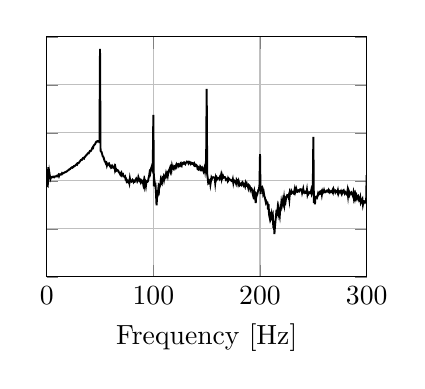
\begin{tikzpicture}

\begin{axis}[%
width=1.6in,
height=1.2in,
at={(0.758in,0.481in)},
scale only axis,
xmin=0,
xmax=300,
xmajorgrids,
ymin=-20,
ymax=80,
ymajorgrids,
yticklabels={\empty},
xlabel={Frequency [Hz]},
axis background/.style={fill=white}
]
\addplot [color=black,solid,line width=0.7pt,forget plot]
  table[row sep=crcr]{%
0	19.6465475215156\\
0.500005208387587	18.0689028800152\\
1.00001041677517	17.8787178041049\\
1.50001562516276	25.6949032993979\\
2.00002083355035	20.741440842814\\
2.50002604193794	23.4436884863118\\
3.00003125032552	21.9987814215028\\
3.50003645871311	20.7551999998466\\
4.0000416671007	21.3442193438068\\
4.50004687548829	21.6225394619914\\
5.00005208387587	21.5767222176182\\
5.50005729226346	21.5231499908941\\
6.00006250065105	21.7779093752474\\
6.50006770903864	21.6259988265967\\
7.00007291742622	21.48686496617\\
7.50007812581381	21.6577112446981\\
8.0000833342014	21.9161773022356\\
8.50008854258899	21.9230224226315\\
9.00009375097657	21.9098357006603\\
9.50009895936416	22.1188383191754\\
10.0001041677517	21.8933084887289\\
10.5001093761393	21.9996068363315\\
11.0001145845269	22.4358100882108\\
11.5001197929145	21.9153405664525\\
12.0001250013021	22.5099355450235\\
12.5001302096897	22.7589992845797\\
13.0001354180773	22.6588616423168\\
13.5001406264649	22.7930475650184\\
14.0001458348524	22.6907494832287\\
14.50015104324	23.2572406147899\\
15.0001562516276	23.0738594674994\\
15.5001614600152	23.1694727003827\\
16.0001666684028	23.272147400615\\
16.5001718767904	23.4566191286534\\
17.000177085178	23.4963488023425\\
17.5001822935656	23.7712124629934\\
18.0001875019531	23.7658786053877\\
18.5001927103407	23.8453731103512\\
19.0001979187283	23.9832465962102\\
19.5002031271159	24.2072667081773\\
20.0002083355035	24.3918504105879\\
20.5002135438911	24.4453502600418\\
21.0002187522787	24.7542782913593\\
21.5002239606663	24.86654694808\\
22.0002291690538	24.9464195490288\\
22.5002343774414	25.2249898632992\\
23.000239585829	25.4239819007627\\
23.5002447942166	25.6144527323529\\
24.0002500026042	25.4834005324954\\
24.5002552109918	25.7567000817357\\
25.0002604193794	25.7549237933793\\
25.500265627767	26.1428850242285\\
26.0002708361545	26.1342413228417\\
26.5002760445421	26.2636280003019\\
27.0002812529297	26.5575791681411\\
27.5002864613173	26.6970239124046\\
28.0002916697049	26.9631299619597\\
28.5002968780925	26.7890898857552\\
29.0003020864801	27.4060286748657\\
29.5003072948677	27.4149550683949\\
30.0003125032552	27.4412158335795\\
30.5003177116428	27.7553685030947\\
31.0003229200304	28.0546402743078\\
31.500328128418	28.3394376600552\\
32.0003333368056	28.6816560666505\\
32.5003385451932	28.7673034411339\\
33.0003437535808	28.7700502066264\\
33.5003489619684	29.1870775069539\\
34.0003541703559	29.4732520067898\\
34.5003593787435	29.4430412763114\\
35.0003645871311	29.309760665553\\
35.5003697955187	29.9473173627193\\
36.0003750039063	30.0303519397308\\
36.5003802122939	30.3792180899321\\
37.0003854206815	30.661710770157\\
37.5003906290691	30.8544832077614\\
38.0003958374566	31.0952780454891\\
38.5004010458442	31.416642071764\\
39.0004062542318	31.6153740488626\\
39.5004114626194	31.5460907033801\\
40.000416671007	31.9873803350387\\
40.5004218793946	32.4377338956709\\
41.0004270877822	32.3999380243447\\
41.5004322961697	32.5276799330314\\
42.0004375045573	32.9212493172855\\
42.5004427129449	33.4477647630675\\
43.0004479213325	33.8815354898795\\
43.5004531297201	33.7449624530585\\
44.0004583381077	34.7110187335686\\
44.5004635464953	34.9260778005212\\
45.0004687548829	35.173018441424\\
45.5004739632705	35.3794665147966\\
46.000479171658	35.9577215280577\\
46.5004843800456	36.3072883915484\\
47.0004895884332	36.2425126651982\\
47.5004947968208	36.576158673455\\
48.0005000052084	36.6278491164089\\
48.500505213596	36.6308747041338\\
49.0005104219836	36.3294296069883\\
49.5005156303711	36.6597781697236\\
50.0005208387587	74.9678524199038\\
50.5005260471463	32.558958726366\\
51.0005312555339	32.2227061034954\\
51.5005364639215	32.0351950985246\\
52.0005416723091	31.1762503904525\\
52.5005468806967	30.2899732868765\\
53.0005520890843	30.1727902215424\\
53.5005572974719	29.5656675930865\\
54.0005625058594	28.6954705596527\\
54.500567714247	28.0586108161089\\
55.0005729226346	27.9393970425912\\
55.5005781310222	27.3012675074352\\
56.0005833394098	27.5545748062779\\
56.5005885477974	26.4123312713662\\
57.000593756185	27.0688187636037\\
57.5005989645725	27.1880634629859\\
58.0006041729601	26.8821519421469\\
58.5006093813477	27.1350449322626\\
59.0006145897353	26.345142814141\\
59.5006197981229	26.0319899159731\\
60.0006250065105	26.2157088347219\\
60.5006302148981	25.4436885839997\\
61.0006354232857	25.5833372361332\\
61.5006406316732	26.1293602647676\\
62.0006458400608	25.6541529720702\\
62.5006510484484	25.7847034383571\\
63.000656256836	25.4859954570159\\
63.5006614652236	26.0012062077558\\
64.0006666736112	24.644952372222\\
64.5006718819988	25.4960002550069\\
65.0006770903864	24.381636487988\\
65.500682298774	24.6856057875452\\
66.0006875071615	24.3238515313446\\
66.5006927155491	24.447287593283\\
67.0006979239367	24.3398656768628\\
67.5007031323243	23.7125088492456\\
68.0007083407119	23.4731695119771\\
68.5007135490995	23.0976589395448\\
69.0007187574871	22.6641785661748\\
69.5007239658746	23.2228031677788\\
70.0007291742622	23.5204157602373\\
70.5007343826498	22.4756137851567\\
71.0007395910374	22.8437580103106\\
71.500744799425	22.9276091943906\\
72.0007500078126	21.8972327215304\\
72.5007552162002	21.883370603806\\
73.0007604245878	21.698316994578\\
73.5007656329753	21.8955641276383\\
74.0007708413629	20.6433874645916\\
74.5007760497505	20.7823600613758\\
75.0007812581381	19.7440386365726\\
75.5007864665257	20.0209833171895\\
76.0007916749133	19.4990899273388\\
76.5007968833009	19.3554034293551\\
77.0008020916885	19.9022063624182\\
77.500807300076	19.0376134904288\\
78.0008125084636	20.9696578916301\\
78.5008177168512	19.7674553175965\\
79.0008229252388	19.8866817911247\\
79.5008281336264	19.7280070946432\\
80.000833342014	20.0195827970292\\
80.5008385504016	20.4642534674218\\
81.0008437587892	20.1910255856036\\
81.5008489671767	19.4684158322989\\
82.0008541755643	19.7654256708112\\
82.5008593839519	19.6739450244728\\
83.0008645923395	20.3683573433978\\
83.5008698007271	20.5699035343044\\
84.0008750091147	20.9848728585917\\
84.5008802175023	20.5584542573532\\
85.0008854258898	19.773468841564\\
85.5008906342774	20.1797658671863\\
86.000895842665	21.555034998247\\
86.5009010510526	20.9117657142011\\
87.0009062594402	20.0537800672136\\
87.5009114678278	19.9277209093655\\
88.0009166762154	19.4309154768267\\
88.500921884603	20.3527831732155\\
89.0009270929906	20.0677578064319\\
89.5009323013781	19.5597325524115\\
90.0009375097657	19.8295048069247\\
90.5009427181533	18.6742059334627\\
91.0009479265409	19.8230910206473\\
91.5009531349285	18.2417939508653\\
92.0009583433161	20.0254887086348\\
92.5009635517037	19.0130208148491\\
93.0009687600913	17.8417050298999\\
93.5009739684788	19.7483032122439\\
94.0009791768664	19.4960111806149\\
94.500984385254	19.6226201320208\\
95.0009895936416	19.9452162886008\\
95.5009948020292	21.1046469888565\\
96.0010000104168	22.0105002177321\\
96.5010052188044	23.5180015175284\\
97.0010104271919	22.9660263131289\\
97.5010156355795	24.2615671004013\\
98.0010208439671	25.3425595376603\\
98.5010260523547	26.0358370259557\\
99.0010312607423	25.1484180485483\\
99.5010364691299	26.8973100228092\\
100.001041677517	47.4970342471067\\
100.501046885905	17.6990734477248\\
101.001052094293	20.1602426161851\\
101.50105730268	18.3369695696015\\
102.001062511068	18.5106911637534\\
102.501067719455	14.5799141943309\\
103.001072927843	9.83818473024378\\
103.501078136231	13.094281245374\\
104.001083344618	13.7812309456733\\
104.501088553006	15.9270236602122\\
105.001093761393	14.0205073384533\\
105.501098969781	17.9393261691097\\
106.001104178169	17.6149140860937\\
106.501109386556	18.3135338531801\\
107.001114594944	20.4033702588398\\
107.501119803331	19.5545390274059\\
108.001125011719	19.1035345757161\\
108.501130220106	21.1668324362358\\
109.001135428494	20.8518160974626\\
109.501140636882	21.6228050915506\\
110.001145845269	20.4526761892544\\
110.501151053657	21.7365911534965\\
111.001156262044	22.2199480636208\\
111.501161470432	21.7648503510144\\
112.00116667882	23.1715207900592\\
112.501171887207	22.4017907529532\\
113.001177095595	22.9559583103322\\
113.501182303982	22.0393994032915\\
114.00118751237	23.4875131080206\\
114.501192720758	24.3479146921007\\
115.001197929145	24.6356155626492\\
115.501203137533	25.2957761783523\\
116.00120834592	24.1873061894031\\
116.501213554308	25.3358842588041\\
117.001218762695	24.4163492715706\\
117.501223971083	26.2668470850821\\
118.001229179471	25.3534366781345\\
118.501234387858	25.2471938309847\\
119.001239596246	24.974697604888\\
119.501244804633	26.2019587562202\\
120.001250013021	26.08535992427\\
120.501255221409	25.5561866130356\\
121.001260429796	26.2145858731329\\
121.501265638184	26.7646056965865\\
122.001270846571	26.0107856134918\\
122.501276054959	26.6847479601111\\
123.001281263347	27.0124138257287\\
123.501286471734	27.07359522186\\
124.001291680122	26.2095384610236\\
124.501296888509	26.5844826917995\\
125.001302096897	26.3717650418245\\
125.501307305284	27.0127036613921\\
126.001312513672	26.5445509734219\\
126.50131772206	26.2648435693202\\
127.001322930447	27.3706304656612\\
127.501328138835	27.1883726336735\\
128.001333347222	27.4549330722423\\
128.50133855561	27.2172516408587\\
129.001343763998	27.6462536664641\\
129.501348972385	27.4517898185102\\
130.001354180773	27.0404869295846\\
130.50135938916	27.5020500960043\\
131.001364597548	27.6445725476375\\
131.501369805935	28.0539492010691\\
132.001375014323	27.9455686838577\\
132.501380222711	27.97707995813\\
133.001385431098	27.2705662959879\\
133.501390639486	27.6095920538507\\
134.001395847873	27.8325941354043\\
134.501401056261	27.4714339681957\\
135.001406264649	27.0953900337184\\
135.501411473036	27.6077960414325\\
136.001416681424	27.5240197254537\\
136.501421889811	27.1870185262116\\
137.001427098199	27.3328928311423\\
137.501432306587	26.9912382056555\\
138.001437514974	26.6401414506376\\
138.501442723362	27.2438644531834\\
139.001447931749	26.8352474865952\\
139.501453140137	26.1367235850483\\
140.001458348524	26.1207174546537\\
140.501463556912	26.4688061496048\\
141.0014687653	26.0988607545565\\
141.501473973687	24.9327976378568\\
142.001479182075	24.7731060485608\\
142.501484390462	25.6406978717471\\
143.00148959885	25.4258082122244\\
143.501494807238	25.0311079210332\\
144.001500015625	26.0293043141694\\
144.501505224013	25.703616579526\\
145.0015104324	24.4028039875191\\
145.501515640788	24.4211881053431\\
146.001520849176	25.214619697856\\
146.501526057563	24.6902359313847\\
147.001531265951	24.0290608743388\\
147.501536474338	24.9083559499639\\
148.001541682726	25.6470360104748\\
148.501546891113	24.1806220442528\\
149.001552099501	26.0305945650593\\
149.501557307889	29.1424839849523\\
150.001562516276	58.3103309838934\\
150.501567724664	22.7728458523502\\
151.001572933051	21.0185152632427\\
151.501578141439	18.9418813414425\\
152.001583349827	19.1353148909799\\
152.501588558214	19.9687615895944\\
153.001593766602	20.2727028417178\\
153.501598974989	18.5446597634321\\
154.001604183377	19.9701617616002\\
154.501609391765	21.3871981824779\\
155.001614600152	20.9048262015307\\
155.50161980854	21.4564489694158\\
156.001625016927	21.5440066251562\\
156.501630225315	21.4123178418401\\
157.001635433702	21.4172506105227\\
157.50164064209	21.2524649968359\\
158.001645850478	19.1807101185037\\
158.501651058865	21.30576644412\\
159.001656267253	20.607727960865\\
159.50166147564	21.3391687250302\\
160.001666684028	20.8430599318868\\
160.501671892416	21.1349345050455\\
161.001677100803	21.2415825488609\\
161.501682309191	21.1695782701221\\
162.001687517578	20.8020315524078\\
162.501692725966	21.6776729131786\\
163.001697934353	21.3586810866509\\
163.501703142741	22.4116863473266\\
164.001708351129	20.9913848263139\\
164.501713559516	22.2335686605146\\
165.001718767904	21.4539124216393\\
165.501723976291	21.9684558295402\\
166.001729184679	21.4018949784003\\
166.501734393067	21.5698707981725\\
167.001739601454	21.5858668582446\\
167.501744809842	21.3179660602234\\
168.001750018229	20.5081304183052\\
168.501755226617	20.7447816560762\\
169.001760435005	20.7861281073225\\
169.501765643392	20.1364223075345\\
170.00177085178	21.0117972163038\\
170.501776060167	20.3979932179332\\
171.001781268555	20.9059818042321\\
171.501786476942	20.6761737383529\\
172.00179168533	20.4729024635418\\
172.501796893718	20.416116720677\\
173.001802102105	20.0895742730252\\
173.501807310493	19.929354260182\\
174.00181251888	19.8013048679317\\
174.501817727268	20.6682840009255\\
175.001822935656	19.1656723125451\\
175.501828144043	20.2759218628866\\
176.001833352431	20.0330555654675\\
176.501838560818	19.9441135257873\\
177.001843769206	19.5333578499262\\
177.501848977594	18.9147432782004\\
178.001854185981	20.3827928251974\\
178.501859394369	19.9238765782401\\
179.001864602756	20.1412131958563\\
179.501869811144	18.9045116548151\\
180.001875019531	19.8925409489276\\
180.501880227919	19.0876770173322\\
181.001885436307	18.1734191109519\\
181.501890644694	18.4107325144131\\
182.001895853082	18.7233505522921\\
182.501901061469	18.3912299959263\\
183.001906269857	19.1332084864658\\
183.501911478245	19.4483447375851\\
184.001916686632	18.9785574385698\\
184.50192189502	18.2188439515816\\
185.001927103407	18.6700219675675\\
185.501932311795	18.4168242937567\\
186.001937520183	17.7598563415002\\
186.50194272857	19.0888376211691\\
187.001947936958	18.4270790863697\\
187.501953145345	18.861090452294\\
188.001958353733	17.9413336704971\\
188.50196356212	17.9877112852056\\
189.001968770508	17.0730367684301\\
189.501973978896	18.2887715077489\\
190.001979187283	18.0752705453601\\
190.501984395671	17.562671333025\\
191.001989604058	16.3721279541278\\
191.501994812446	17.0521700042665\\
192.002000020834	16.8929288529771\\
192.502005229221	16.364587667449\\
193.002010437609	14.8330603877504\\
193.502015645996	13.9535410802419\\
194.002020854384	14.814885633027\\
194.502026062771	12.300880222239\\
195.002031271159	14.4962771467503\\
195.502036479547	12.7930733988172\\
196.002041687934	10.7813593512685\\
196.502046896322	14.3198040521445\\
197.002052104709	13.9342804571412\\
197.502057313097	14.535666516131\\
198.002062521485	15.5415840684445\\
198.502067729872	16.2828116762858\\
199.00207293826	16.3341262024934\\
199.502078146647	18.3560919343135\\
200.002083355035	31.1262225443117\\
200.502088563423	14.4953359235955\\
201.00209377181	16.8197241368359\\
201.502098980198	17.3368154540174\\
202.002104188585	17.4961318690493\\
202.502109396973	16.8688527495506\\
203.00211460536	14.6173360500943\\
203.502119813748	15.2100323786826\\
204.002125022136	13.8315025792699\\
204.502130230523	13.0931295898009\\
205.002135438911	12.0810572098132\\
205.502140647298	10.9497466685868\\
206.002145855686	11.4780312230313\\
206.502151064074	10.9880667406085\\
207.002156272461	10.9784965966466\\
207.502161480849	8.08382163620812\\
208.002166689236	10.2478474928266\\
208.502171897624	5.91573870983216\\
209.002177106012	4.82087438528686\\
209.502182314399	7.14761902988004\\
210.002187522787	3.97027945377215\\
210.502192731174	4.52037054973538\\
211.002197939562	6.17267076712241\\
211.502203147949	4.91527719979677\\
212.002208356337	5.61575544294\\
212.502213564725	0.411801943740878\\
213.002218773112	2.5316020738186\\
213.5022239815	-2.10796006754471\\
214.002229189887	0.917013792040361\\
214.502234398275	3.34277907306545\\
215.002239606663	5.4349284222104\\
215.50224481505	8.01145057614835\\
216.002250023438	5.50482430379487\\
216.502255231825	8.27277218189767\\
217.002260440213	6.64032615375849\\
217.502265648601	8.41218234892338\\
218.002270856988	6.62371101963924\\
218.502276065376	5.4303160040749\\
219.002281273763	8.4010517132806\\
219.502286482151	8.58337218440875\\
220.002291690538	10.9372172162179\\
220.502296898926	9.61368928116577\\
221.002302107314	10.7048135989229\\
221.502307315701	12.0199890213592\\
222.002312524089	10.9046723718199\\
222.502317732476	12.7205074172932\\
223.002322940864	10.4694361140755\\
223.502328149252	12.2321044932087\\
224.002333357639	11.542271252635\\
224.502338566027	13.1557882665086\\
225.002343774414	13.5959950691783\\
225.502348982802	14.1057314823393\\
226.002354191189	14.0576433725324\\
226.502359399577	13.3855371353586\\
227.002364607965	14.1274122033769\\
227.502369816352	12.3717989459305\\
228.00237502474	15.1406907377798\\
228.502380233127	14.4785489617822\\
229.002385441515	14.552203467205\\
229.502390649903	15.8276960826969\\
230.00239585829	15.4201722741973\\
230.502401066678	15.1793515360241\\
231.002406275065	14.8873473671469\\
231.502411483453	14.7251051136492\\
232.002416691841	15.5288441876042\\
232.502421900228	16.5681846282201\\
233.002427108616	15.2606093983403\\
233.502432317003	15.9649355660759\\
234.002437525391	16.7404189198625\\
234.502442733778	15.9292525717537\\
235.002447942166	15.4074392780873\\
235.502453150554	15.529260092396\\
236.002458358941	16.0976685774788\\
236.502463567329	16.15625571731\\
237.002468775716	15.8379710325949\\
237.502473984104	16.4459399986971\\
238.002479192492	16.5401270147836\\
238.502484400879	16.5119794921784\\
239.002489609267	16.3629630734446\\
239.502494817654	15.0389896656505\\
240.002500026042	15.8596336332357\\
240.50250523443	16.7170344421455\\
241.002510442817	15.2838576907536\\
241.502515651205	15.4525743113001\\
242.002520859592	15.0575449003716\\
242.50252606798	15.333241553271\\
243.002531276367	15.0129370181341\\
243.502536484755	14.9699345622894\\
244.002541693143	16.2938728799102\\
244.50254690153	14.3596063920793\\
245.002552109918	15.154854039406\\
245.502557318305	14.6163038257227\\
246.002562526693	15.0088893476277\\
246.502567735081	15.2441216750787\\
247.002572943468	15.0586493834032\\
247.502578151856	14.8911237665164\\
248.002583360243	16.0031273545241\\
248.502588568631	14.6786373596327\\
249.002593777019	15.3846811157934\\
249.502598985406	16.6514218542466\\
250.002604193794	38.3815794587938\\
250.502609402181	10.8134645669834\\
251.002614610569	12.2104258639038\\
251.502619818956	10.2532203660415\\
252.002625027344	13.1525672322588\\
252.502630235732	13.4206147631903\\
253.002635444119	13.3983917974799\\
253.502640652507	13.0798296344517\\
254.002645860894	13.8731478640882\\
254.502651069282	14.7910643488725\\
255.00265627767	14.2907630913756\\
255.502661486057	14.5486331300483\\
256.002666694445	15.1783145854907\\
256.502671902832	14.9231004536801\\
257.00267711122	15.6742654294423\\
257.502682319608	15.8634793404994\\
258.002687527995	14.3534979810168\\
258.502692736383	15.6922829831678\\
259.00269794477	15.0668969263543\\
259.502703153158	15.4159515258958\\
260.002708361545	16.1423176876857\\
260.502713569933	15.3319626773771\\
261.002718778321	15.2327759920027\\
261.502723986708	15.2920990199983\\
262.002729195096	15.5260693515302\\
262.502734403483	15.9960596284667\\
263.002739611871	16.021112059921\\
263.502744820259	15.5494619094033\\
264.002750028646	15.407658967013\\
264.502755237034	16.2366305306734\\
265.002760445421	15.8655754815972\\
265.502765653809	15.2845853609619\\
266.002770862196	15.6678121210198\\
266.502776070584	15.5089751921883\\
267.002781278972	15.7080226435799\\
267.502786487359	15.3833138897537\\
268.002791695747	16.0404840233516\\
268.502796904134	15.3305346555628\\
269.002802112522	16.5153327612845\\
269.50280732091	15.910584586031\\
270.002812529297	15.8411946589148\\
270.502817737685	15.2777795267849\\
271.002822946072	15.8427988796331\\
271.50282815446	15.583729330914\\
272.002833362848	15.6972153653119\\
272.502838571235	15.188890181286\\
273.002843779623	16.0423940417517\\
273.50284898801	14.6439256019564\\
274.002854196398	15.2715864399897\\
274.502859404785	15.5708134649029\\
275.002864613173	15.3518540019106\\
275.502869821561	15.6641934885329\\
276.002875029948	15.1121531815712\\
276.502880238336	14.5898484640178\\
277.002885446723	15.6217528285315\\
277.502890655111	15.2143398095514\\
278.002895863499	15.7333236215094\\
278.502901071886	16.0287101307488\\
279.002906280274	15.398317752049\\
279.502911488661	14.7362044284685\\
280.002916697049	15.1821229278559\\
280.502921905436	14.7787063155321\\
281.002927113824	14.8051498202561\\
281.502932322212	14.4057181033105\\
282.002937530599	15.8364394380393\\
282.502942738987	13.907701541751\\
283.002947947374	16.1438551319664\\
283.502953155762	15.5664819846537\\
284.00295836415	14.1701665955445\\
284.502963572537	14.6994935734202\\
285.002968780925	14.83095712106\\
285.502973989312	15.1277647574674\\
286.0029791977	14.4979762074893\\
286.502984406088	14.2999948714145\\
287.002989614475	13.7443745816358\\
287.502994822863	14.9261156013033\\
288.00300003125	12.9774551571866\\
288.503005239638	14.1046132585333\\
289.003010448026	12.8525345856862\\
289.503015656413	14.1996459285575\\
290.003020864801	13.1072882080763\\
290.503026073188	13.7939884381407\\
291.003031281576	12.7564434860385\\
291.503036489963	13.4443329501562\\
292.003041698351	13.6883548227491\\
292.503046906739	12.7626773100922\\
293.003052115126	11.7694621512106\\
293.503057323514	11.9980048963281\\
294.003062531901	12.9665260791084\\
294.503067740289	10.858903147996\\
295.003072948677	11.3338019320151\\
295.503078157064	11.913312804121\\
296.003083365452	12.3933208340217\\
296.503088573839	10.2278867958775\\
297.003093782227	11.3702599665779\\
297.503098990614	11.551443985478\\
298.003104199002	11.4722811120582\\
298.50310940739	11.0140945556052\\
299.003114615777	11.3277406022607\\
299.503119824165	11.4490256255272\\
300.003125032552	22.347890268008\\
};
\end{axis}
\end{tikzpicture}%
    \caption{Measurement 12 (mic).}
    \label{fig:FFT_mic1_50Hz}
\end{subfigure}
\caption{Frequency response of 50 Hz (a) measurement 1 from the microphone, (b) measurement 6 from the microphone, and (c) measurement 12 from the microphone. Test 2.}
\label{fig:FFT_mic1612}
\end{figure}   

If the amplitudes of the keynote, second harmonic and third harmonic is located at every soundlevel a comparison can be made between the amplitude of:
\begin{itemize}
\item Keynote / Second harmonic
\item Keynote / Third harmonic
\end{itemize}
This should be done for every frequency, but as an example the comparison for 50 Hz is shown in \autoref{fig:com_mic1213}.

\begin{figure}[H]
\centering
\begin{subfigure}[t]{0.45\textwidth}
    \tikzsetnextfilename{comp_mic12}
    % This file was created by matlab2tikz.
%
%The latest updates can be retrieved from
%  http://www.mathworks.com/matlabcentral/fileexchange/22022-matlab2tikz-matlab2tikz
%where you can also make suggestions and rate matlab2tikz.
%
\definecolor{mycolor1}{rgb}{0.00000,0.44700,0.74100}%
%
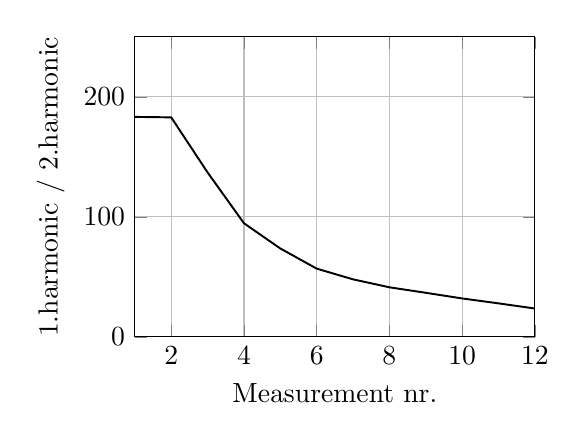
\begin{tikzpicture}

\begin{axis}[%
width=2.0in,
height=1.5in,
at={(0.758in,0.481in)},
scale only axis,
xmin=1,
xmax=12,
xmajorgrids,
ymin=0,
ymax=250,
ymajorgrids,
ylabel={1.harmonic / 2.harmonic},
xlabel={Measurement nr.},
axis background/.style={fill=white}
]
\addplot [color=black,solid,line width=0.7pt,forget plot]
  table[row sep=crcr]{%
1	183.31499672752\\
2	182.923283347804\\
3	137.013097236793\\
4	94.6925534942438\\
5	73.6612276153094\\
6	56.869474600648\\
7	47.9404158862649\\
8	41.3127455693234\\
9	36.731978854038\\
10	32.0273531547799\\
11	27.9256094731595\\
12	23.634200124928\\
};
\end{axis}
\end{tikzpicture}%
    \caption{1.harmonic / 2.harmonic pr. measurement.}
    \label{fig:comp_mic12}
\end{subfigure}
\begin{subfigure}[t]{0.45\textwidth}
    \tikzsetnextfilename{comp_mic13}
    % This file was created by matlab2tikz.
%
%The latest updates can be retrieved from
%  http://www.mathworks.com/matlabcentral/fileexchange/22022-matlab2tikz-matlab2tikz
%where you can also make suggestions and rate matlab2tikz.
%
\definecolor{mycolor1}{rgb}{0.00000,0.44700,0.74100}%
%
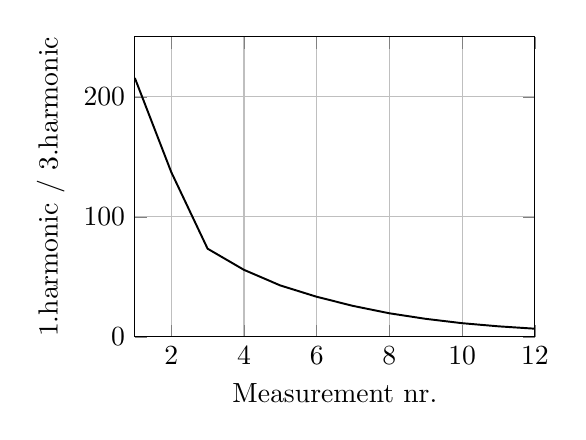
\begin{tikzpicture}

\begin{axis}[%
width=2.0in,
height=1.5in,
at={(0.758in,0.481in)},
scale only axis,
xmin=1,
xmax=12,
xmajorgrids,
ymin=0,
ymax=250,
ymajorgrids,
ylabel={1.harmonic / 3.harmonic},
xlabel={Measurement nr.},
axis background/.style={fill=white}
]
\addplot [color=black,solid,line width=0.7pt,forget plot]
  table[row sep=crcr]{%
1	215.719482689042\\
2	137.375839651914\\
3	73.491881974411\\
4	55.8600092831965\\
5	42.8578352198597\\
6	33.4172800378876\\
7	25.8045950665186\\
8	19.6476489187032\\
9	15.0203405516948\\
10	11.4021105008808\\
11	8.78151310064488\\
12	6.80575125314477\\
};
\end{axis}
\end{tikzpicture}%
    \caption{1.harmonic / 3.harmonic pr. measurement.}
    \label{fig:comp_mic13}
\end{subfigure}
\caption{comparison of keynote (1.harmonic), second harmoni and third harmonic (a) 1.harmonic [mag] / 2.harmonic [mag] and (b) 1.harmonic [mag] / 3.harmonic [mag]. Test 2.}
\label{fig:com_mic1213}
\end{figure}   

It can be derived from \autoref{fig:com_mic1213} that the relation between the keynote and the second harmonic as seen in \autoref{fig:comp_mic12} goes torward 1 at a slower pace than the keynote in relationship to the thirdharmonic as seen in \autoref{fig:comp_mic13} goes torward 1. This corresponds to the theory that when the loudspeaker starts to distort the third harmonic rises quicker than the second harmonic. To control that every frequency has the same pattern as 50 Hz they are all plotted into a singe figure as seen on \autoref{fig:com_mic12All} and \autoref{fig:com_mic13All}

\begin{figure}[H]
    \centering
    \tikzsetnextfilename{comp_mic12All1}
    % This file was created by matlab2tikz.
%
%The latest updates can be retrieved from
%  http://www.mathworks.com/matlabcentral/fileexchange/22022-matlab2tikz-matlab2tikz
%where you can also make suggestions and rate matlab2tikz.
%
\definecolor{mycolor1}{rgb}{0.00000,0.44700,0.74100}%
\definecolor{mycolor2}{rgb}{0.85000,0.32500,0.09800}%
\definecolor{mycolor3}{rgb}{0.92900,0.69400,0.12500}%
\definecolor{mycolor4}{rgb}{0.49400,0.18400,0.55600}%
\definecolor{mycolor5}{rgb}{0.46600,0.67400,0.18800}%
\definecolor{mycolor6}{rgb}{0.30100,0.74500,0.93300}%
\definecolor{mycolor7}{rgb}{0.63500,0.07800,0.18400}%
%
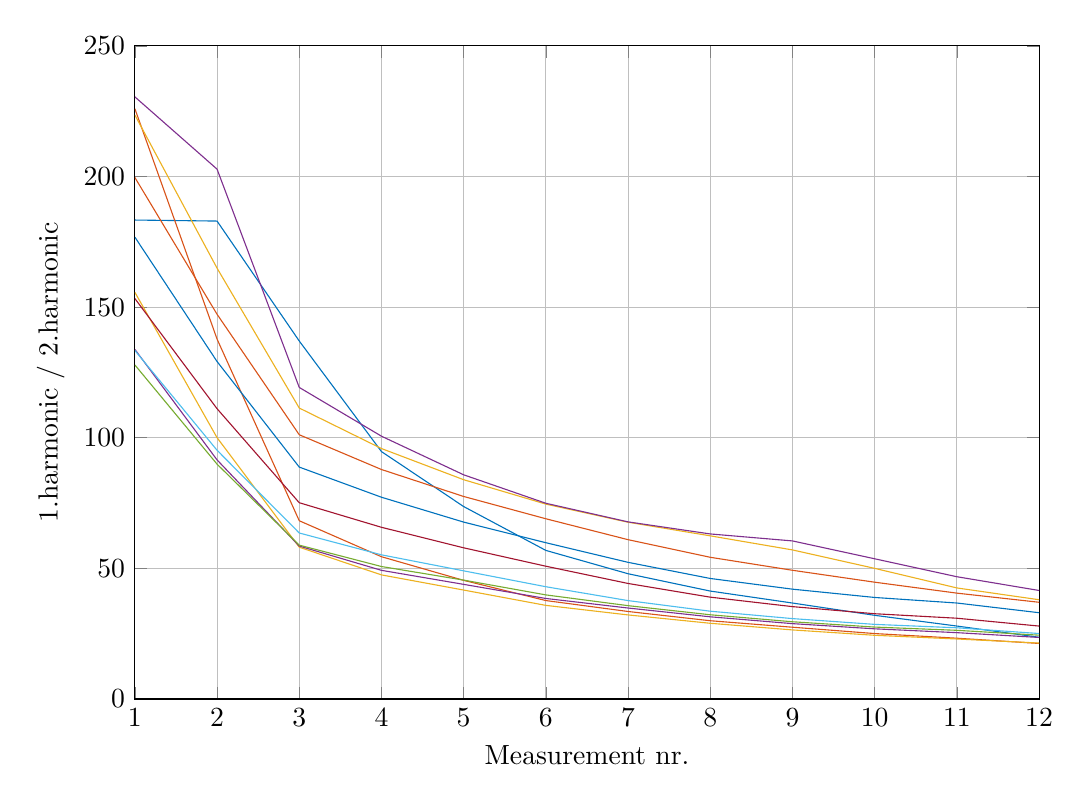
\begin{tikzpicture}

\begin{axis}[%
width=4.521in,
height=3.266in,
at={(0.758in,0.481in)},
scale only axis,
xmin=1,
xmax=12,
xmajorgrids,
ymin=0,
ymax=250,
ymajorgrids,
ylabel={1.harmonic / 2.harmonic},
xlabel={Measurement nr.},
legend style={legend cell align=left,align=left,draw=white!15!black},
every axis legend/.code={\let\addlegendentry\relax},
axis background/.style={fill=white}
]
\addplot [color=mycolor1,solid]
  table[row sep=crcr]{%
1	183.31499672752\\
2	182.923283347804\\
3	137.013097236793\\
4	94.6925534942438\\
5	73.6612276153094\\
6	56.869474600648\\
7	47.9404158862649\\
8	41.3127455693234\\
9	36.731978854038\\
10	32.0273531547799\\
11	27.9256094731595\\
12	23.634200124928\\
};
\addlegendentry{50 Hz};

\addplot [color=mycolor2,solid]
  table[row sep=crcr]{%
1	225.948651932867\\
2	137.755050018691\\
3	68.2246363346026\\
4	54.4579559584202\\
5	45.4083554922301\\
6	37.6766259171707\\
7	33.4934224545393\\
8	29.9560105655195\\
9	27.4727577951372\\
10	25.047988665373\\
11	23.2683916304266\\
12	21.2612643900937\\
};
\addlegendentry{55 Hz};

\addplot [color=mycolor3,solid]
  table[row sep=crcr]{%
1	155.678149120929\\
2	100.022797831327\\
3	58.1057401069468\\
4	47.4987178245013\\
5	41.6971616530277\\
6	35.8331506839115\\
7	32.1786146045458\\
8	28.9797452592156\\
9	26.4372197242896\\
10	24.3848437971063\\
11	22.9713052574951\\
12	21.4168406468615\\
};
\addlegendentry{60 Hz};

\addplot [color=mycolor4,solid]
  table[row sep=crcr]{%
1	133.817626421829\\
2	91.5149244833714\\
3	58.5384949852238\\
4	49.2470691552335\\
5	43.8775896806023\\
6	38.4768722430212\\
7	34.8207269445509\\
8	31.4540583854983\\
9	28.8475989714235\\
10	26.858844097433\\
11	25.3934919568873\\
12	23.556552263722\\
};
\addlegendentry{65 Hz};

\addplot [color=mycolor5,solid]
  table[row sep=crcr]{%
1	127.861211242644\\
2	89.889445285672\\
3	58.8879200629259\\
4	50.7070495285756\\
5	45.5030311570562\\
6	39.8435660751046\\
7	35.72801565913\\
8	32.2386181163127\\
9	29.5646511483646\\
10	27.5293459172169\\
11	26.2885725548033\\
12	24.4334730867523\\
};
\addlegendentry{70 Hz};

\addplot [color=mycolor6,solid]
  table[row sep=crcr]{%
1	133.411971221179\\
2	95.2057327932536\\
3	63.5367427328931\\
4	55.1817402775643\\
5	49.0515929982958\\
6	42.9695998229895\\
7	37.6619270192647\\
8	33.6048133184697\\
9	30.7707384789897\\
10	28.5630272790279\\
11	27.2591841658995\\
12	25.0599352043113\\
};
\addlegendentry{75 Hz};

\addplot [color=mycolor7,solid]
  table[row sep=crcr]{%
1	153.2812963578\\
2	111.103381482628\\
3	75.1222297536225\\
4	65.7170950517263\\
5	57.866990747027\\
6	50.8238512280319\\
7	44.2207437848813\\
8	38.9799605093079\\
9	35.3554040226597\\
10	32.6367123733719\\
11	30.9179484446488\\
12	27.9148240542393\\
};
\addlegendentry{80 Hz};

\addplot [color=mycolor1,solid]
  table[row sep=crcr]{%
1	176.785975612244\\
2	129.168929912779\\
3	88.7614425639971\\
4	77.222188304434\\
5	67.7061040724528\\
6	59.8164235899326\\
7	52.3070636342814\\
8	46.1325579949139\\
9	42.0396260507615\\
10	38.8635031735388\\
11	36.7345650452588\\
12	33.0260180452955\\
};
\addlegendentry{85 Hz};

\addplot [color=mycolor2,solid]
  table[row sep=crcr]{%
1	199.615331947091\\
2	147.252140225702\\
3	101.141987493468\\
4	87.8370948523775\\
5	77.5159470921786\\
6	68.9835361998863\\
7	60.9797782057243\\
8	54.2371635551906\\
9	49.2658337160926\\
10	44.7075203436336\\
11	40.5224538025861\\
12	37.0187341345769\\
};
\addlegendentry{90 Hz};

\addplot [color=mycolor3,solid]
  table[row sep=crcr]{%
1	223.522576176801\\
2	164.894852775071\\
3	111.363739550245\\
4	95.8631283577604\\
5	83.9301003926259\\
6	74.5890678821833\\
7	67.6549025382935\\
8	62.4484355431693\\
9	57.0583739697046\\
10	50.000034475036\\
11	42.5114924874639\\
12	37.9904265344149\\
};
\addlegendentry{95 Hz};

\addplot [color=mycolor4,solid]
  table[row sep=crcr]{%
1	230.461178899143\\
2	202.793651245738\\
3	119.246105525346\\
4	100.588202896866\\
5	85.8077314609676\\
6	74.91091078059\\
7	67.7902618100588\\
8	63.1737027698069\\
9	60.5033449147164\\
10	53.6679215179322\\
11	46.7964660982811\\
12	41.5446189375712\\
};
\addlegendentry{100 Hz};

\end{axis}
\end{tikzpicture}%
    \caption{1.harmonic / 2.harmonic pr. measurement. comparison for all frequencies}
\label{fig:com_mic12All}
\end{figure}   
\begin{figure}[H]
    \centering
    \tikzsetnextfilename{comp_mic13All1}
    % This file was created by matlab2tikz.
%
%The latest updates can be retrieved from
%  http://www.mathworks.com/matlabcentral/fileexchange/22022-matlab2tikz-matlab2tikz
%where you can also make suggestions and rate matlab2tikz.
%
\definecolor{mycolor1}{rgb}{0.00000,0.44700,0.74100}%
\definecolor{mycolor2}{rgb}{0.85000,0.32500,0.09800}%
\definecolor{mycolor3}{rgb}{0.92900,0.69400,0.12500}%
\definecolor{mycolor4}{rgb}{0.49400,0.18400,0.55600}%
\definecolor{mycolor5}{rgb}{0.46600,0.67400,0.18800}%
\definecolor{mycolor6}{rgb}{0.30100,0.74500,0.93300}%
\definecolor{mycolor7}{rgb}{0.63500,0.07800,0.18400}%
%
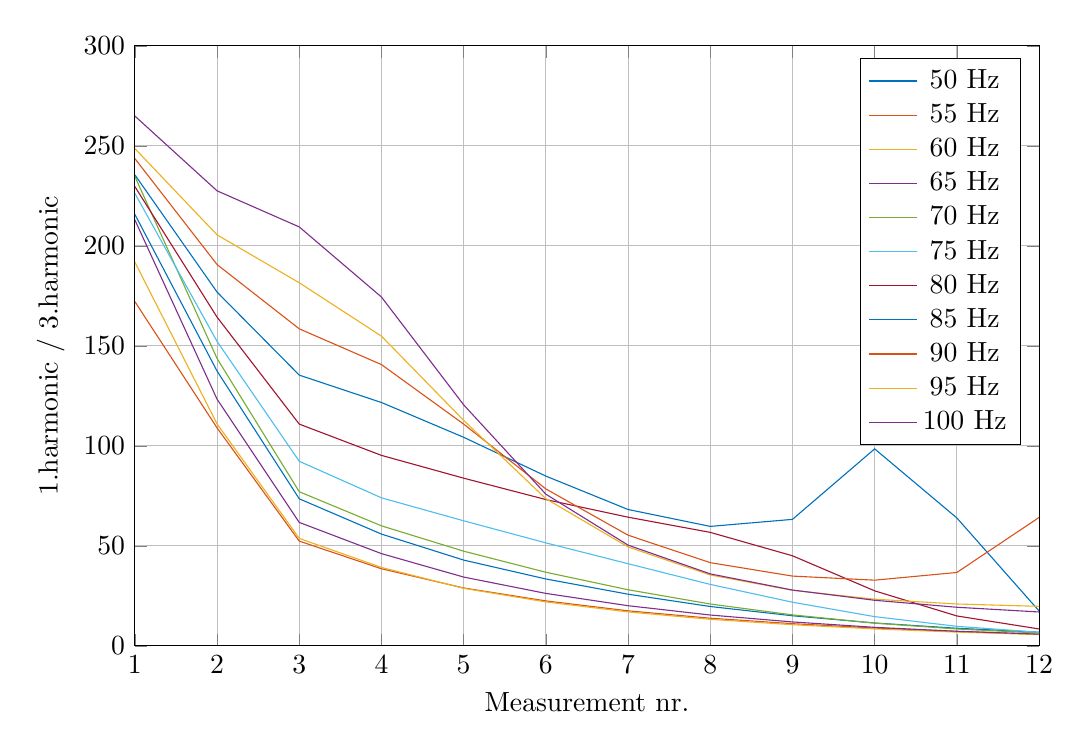
\begin{tikzpicture}

\begin{axis}[%
width=4.521in,
height=3in,
at={(0.758in,0.481in)},
scale only axis,
xmin=1,
xmax=12,
xmajorgrids,
ymin=0,
ymax=300,
ymajorgrids,
ylabel={1.harmonic / 3.harmonic},
xlabel={Measurement nr.},
axis background/.style={fill=white}
]
\addplot [color=mycolor1,solid]
  table[row sep=crcr]{%
1	215.719482689042\\
2	137.375839651914\\
3	73.491881974411\\
4	55.8600092831965\\
5	42.8578352198597\\
6	33.4172800378876\\
7	25.8045950665186\\
8	19.6476489187032\\
9	15.0203405516948\\
10	11.4021105008808\\
11	8.78151310064488\\
12	6.80575125314477\\
};
\addlegendentry{50 Hz};

\addplot [color=mycolor2,solid]
  table[row sep=crcr]{%
1	172.114474693239\\
2	108.959681506917\\
3	52.3472860469133\\
4	38.5211919605244\\
5	28.9212327445786\\
6	22.4544179872231\\
7	17.4931667868384\\
8	13.801173223079\\
9	11.0695402422613\\
10	8.86672628119122\\
11	7.18230155557047\\
12	5.85814167806323\\
};
\addlegendentry{55 Hz};

\addplot [color=mycolor3,solid]
  table[row sep=crcr]{%
1	191.855800187184\\
2	110.953017277433\\
3	53.683693987778\\
4	39.1905573675628\\
5	28.7432207660826\\
6	21.9384090830466\\
7	16.9403111162619\\
8	13.2430949708588\\
9	10.5478998664765\\
10	8.44228317755285\\
11	6.8502781275488\\
12	5.61256508528794\\
};
\addlegendentry{60 Hz};

\addplot [color=mycolor4,solid]
  table[row sep=crcr]{%
1	212.967593013927\\
2	123.29628240462\\
3	61.6977581937471\\
4	46.087964403812\\
5	34.3674120619029\\
6	26.2006981358897\\
7	20.0496847996708\\
8	15.3920698020736\\
9	11.9375533950336\\
10	9.2331507973757\\
11	7.26857819425135\\
12	5.81724097588744\\
};
\addlegendentry{65 Hz};

\addplot [color=mycolor5,solid]
  table[row sep=crcr]{%
1	234.702654081076\\
2	143.654071251651\\
3	77.0302711130303\\
4	59.9879332842773\\
5	47.3106009863147\\
6	36.7764664566778\\
7	28.0333423931352\\
8	20.8956209974193\\
9	15.4637596342843\\
10	11.3278856361071\\
11	8.40468415229921\\
12	6.38901276926542\\
};
\addlegendentry{70 Hz};

\addplot [color=mycolor6,solid]
  table[row sep=crcr]{%
1	226.209153737198\\
2	152.210426408944\\
3	92.2545328200555\\
4	73.9825383217611\\
5	62.5040084794028\\
6	51.4667509935922\\
7	41.049495369253\\
8	30.6957852407747\\
9	21.7968693650809\\
10	14.5785490688354\\
11	9.7443318755874\\
12	6.7525393990427\\
};
\addlegendentry{75 Hz};

\addplot [color=mycolor7,solid]
  table[row sep=crcr]{%
1	229.635293191795\\
2	164.339841957498\\
3	110.849225518279\\
4	95.2095843851408\\
5	83.8160696235361\\
6	73.1256889751953\\
7	64.3117819142494\\
8	56.7158231404608\\
9	45.0103733731685\\
10	27.480243912524\\
11	14.9274558888611\\
12	8.42340571546528\\
};
\addlegendentry{80 Hz};

\addplot [color=mycolor1,solid]
  table[row sep=crcr]{%
1	235.490142481433\\
2	176.874977155834\\
3	135.353253187891\\
4	121.654914199797\\
5	104.262795163307\\
6	84.8518375205328\\
7	68.153561437247\\
8	59.7049006381259\\
9	63.2192417248968\\
10	98.4705122104372\\
11	63.9227101729301\\
12	17.4365884138633\\
};
\addlegendentry{85 Hz};

\addplot [color=mycolor2,solid]
  table[row sep=crcr]{%
1	243.625116326288\\
2	190.625692275955\\
3	158.487616772918\\
4	140.613342268007\\
5	110.851821081734\\
6	78.4408481270658\\
7	55.3137703046313\\
8	41.567805737901\\
9	34.8603436700427\\
10	32.8193125376356\\
11	36.6722236082736\\
12	64.1801894559288\\
};
\addlegendentry{90 Hz};

\addplot [color=mycolor3,solid]
  table[row sep=crcr]{%
1	248.626858493455\\
2	205.485109505812\\
3	181.517854932663\\
4	154.824971458371\\
5	112.734503287044\\
6	73.5428507994872\\
7	49.4273612797893\\
8	35.4248581541094\\
9	27.7586461995489\\
10	23.3064114126667\\
11	20.9043305865742\\
12	19.7354496791802\\
};
\addlegendentry{95 Hz};

\addplot [color=mycolor4,solid]
  table[row sep=crcr]{%
1	264.893936681882\\
2	227.491544249115\\
3	209.43939847287\\
4	174.38343883648\\
5	120.48310284721\\
6	75.8068005942284\\
7	50.3376273635925\\
8	35.9571675595305\\
9	27.8773577027189\\
10	22.7572946932365\\
11	19.2742309190579\\
12	16.9124632980934\\
};
\addlegendentry{100 Hz};

\end{axis}
\end{tikzpicture}%
    \caption{1.harmonic / 3.harmonic pr. measurement. comparison for all frequencies}
\label{fig:com_mic13All}
\end{figure}  

It can be seen on the figures that a pattern can be seen as in figure \autoref{fig:com_mic1213} which goes toward 1. An error in \autoref{fig:com_mic13All} can be seen where the 85 Hz measurement does not follow the pattern of the other frequency which is deemed an error. From \autoref{fig:com_mic12All} and \autoref{fig:com_mic13All} it can be derived that a model can be derived because there is a correlation between the keynote and the second and third harmonic in the frequency spectrum 50 Hz - 100 Hz. The figures shown in the analysis is only based on the microphone measurements. The derived data from the acceloremeters can be found on \textbf{TBD}. The reason for not showing them in this analysis is because they show approximately the same as the microphone but with larger error margin. 


\section{Error sources}
Few errors could have occurred during trials, since then only variable adjusted during between measurements were the gain of the amplifier. There were however problems with moving the setup from the control room were it was calibrated and then moved into the anechoic room. The
calibration was done using an visual equalizer where the output was shown with a bar chart. Hence the data should bee seen with a tolerance of +/- 0.5 dB.

\section{Conclusion}

From these test it can be concluded that the speaker dose not create any significant ''hit pattern'' when different tones a played. It can however be concluded that the speaker has an increase in THD when the amplification is increased. This creates basis for determination of model to predict how the speaker will react to a specific amplification at a specific frequency.  Futhermore it shows that less precise sparkfun accelerometer can not create a usable output. 